\documentclass[oneside,12pt,fleqn]{memoir}

\usepackage{makeidx}
\usepackage[columns=1]{idxlayout}
%\usepackage[utf8]{inputenc}
\pagestyle{plain}
\binoppenalty2000 \relpenalty2000

%%%%%%%%%%%%%%%%%%%%%%%%%%%%%%%%%%%% importa pacchetti
\usepackage{usepkg}
%%%%%%%%%%%%%%%%%%%%%%%%%%%%%%%%%%%%% fancyhdr
\usepackage{fancyfoot}
%%%%%%%%%%%%%%%%%% titletoc, titlesec setting
\usepackage{titleT}
%%%%%%%%%%%%%%%%%% setlength
\usepackage{mylength}
\linespread{0.5}

%%%%%%%%%%%% Hyperref package
\usepackage{hyperref}
\hypersetup{colorlinks,
linktoc=all,
linkcolor=black,
    citecolor=black,
    filecolor=black,
    urlcolor=black
}
%%%%%%%%%%%%%%%%%%%%%%%%

%%%%%%%%%%%%%%%%%Geometry package
\usepackage{mygeometry}

%%%%%%%%%%%%%%%%%%%%%%%%%%%%%%%%%%% Funzioni per questo file main
\usepackage{LocalF}
%%%%%%%%%%%%%%%%%%%%%%%%%%%%%%%%%%% Funzioni generali
\usepackage{functions}
%http://tex.stackexchange.com/questions/246/when-should-i-use-input-vs-include
\usepackage{sources}
\usepackage{MathOp}
%%%%%%%%%%%%%%%%%%%%%%%%%%%%%%%%%
%\usepackage{tikz/data}%%import table for tikz pgfplot


\makeindex
\raggedbottom %http://tex.stackexchange.com/questions/102084/annoying-paragraph-spacing-issue-with-memoir 


%%%%%%%%%%%%%%%%%% Import mypackages
%\usepackage{mytitletoc} %% Remeber some problems occurs if you put this after packages
%\usepackage{packages}   %%
%\usepackage{mygeometry} %%
%\usepackage{functions}  %%
%\usepackage{LocalF} %%
%\usepackage{MathOp} %%
%%%%%%%%%%%%%%%%%%% Sources
%\usepackage{sources}
%%%%%%%%%%%%



\author{Pippetta}
\title{Astro Phys 1}
\date{\today}
%\date{\currenttime}

\makeindex
\raggedbottom %http://tex.stackexchange.com/questions/102084/annoying-paragraph-spacing-issue-with-memoir

%\csname @addtoreset\endcsname{figure}{chapter}

\begin{document}

\frontmatter
\maketitle
\addtocontents{toc}{\protect\hypertarget{toc}{}}
\tableofcontents*

\mainmatter


\part{Costanti e grandezze fisiche e fattori di conversione (che \'e meglio ricordare)}
 

\documentclass[main.tex]{subfiles}

\begin{document}

\chapter{Sole, Terra, stelle, pianeti: dimensioni caratteristiche}
\PartialToc

\section{Sole}

\subsection{Massa e densit\'a}
\begin{itemize*}
\item $\msun\approx1.989*10^{30}\,Kg$
\item $\rhosun\approx1.408 \, gr/cm^3$
\end{itemize*}

\begin{itemize*}
\item $\rsun=6.96*10^8\,m$
\end{itemize*}
\begin{itemize*}
\item $\msun\approx1.989*10^{30}\,Kg$
\item $\rhosun\approx1.408 \, gr/cm^3$
\end{itemize*}

\subsection{G-nal potential energy}

\begin{equation*}
\Omega=\frac{G\msun^2}{\rsun}\approx\num{3.8e48}\si{\erg}
\end{equation*}

\subsection{superficie}

\begin{itemize*}
\item $\gsun=\frac{G\msun}{\rsun^2}=274\,m/s^2$
\end{itemize*}

\subsection{Solar constant}

Solar radiation constant at \SI{1}{\astronomicalunit}
\begin{align*}
&F_0=\SI{1.366e7}{\erg\per\square\cm\per\second}\\
&=\SI{1.366e3}{\joule\per\square\meter\per\second}
\end{align*}


\section{Terra}


\subsection{Massa e densit\'a}

\begin{equation*}
\mT=5.972\sci{27}\,g=5.972\sci{24}\,Kg
\end{equation*}

\subsection{Mean Earth radius}

\begin{equation*}
\rT=6.371\sci{8}\,cm=6.371\sci{6}m
\end{equation*}

\subsection{Oblateness coefficient}

\begin{equation*}
J_2=\frac{C-A}{\mT\rT^2}
\end{equation*}


\subsection{Obliquity at standard epoch}

\begin{align*}
\epsilon=\ang{23;26;21}&\intertext{At standard epoch $J2000.0$}
\end{align*}

\subsection{Lunisolar precession constant}
Rate at which the the vernal equinox point or $gamma$ point intersection between the celestial equator and ecliptic moves along the latter
\begin{equation*}
\Omega_{pr}=\ang{;;50.291}/yr=7.726\sci{-12}\,rad/s
\end{equation*}

\subsection{Sideral angular velocity and secular decreases}

Rotation of Earth on its axis.

\begin{align*}
\roT=(7.2921\sci{-5}-1.4\sci{-14}T)\si{\radian \per \second}&\intertext{T in years}
\end{align*}


 
\section{Masse e densit\'a caratteristiche}

\subsection{White dwarf}

\subsection{Galaxy}


\section{Angoli}

\begin{itemize*}
\item arcosecondo $1''=4.848\sci{-6}\,rad$
\item 1 degree ($\degree$) = \ang{;60;} = \ang{;;3600}
\item \SI{1}{\radian} = \ang{57.296;;} = \ang{;;206265}
\item \SI{1}{\steradian} = \SI{1}{\square\radian} = \SI{3282.8}{\square\deg} = \SI{4.25e10}{\square\arcsec}, where $4\pi$ steradians is the sphere.

\end{itemize*}


\section{Stelle}


\chapter{Energie, frequenze, lunghezze:unit\'a di misura.}
\PartialToc

\section{Unit\'a di misura}

\subsection{Energia}

\begin{align*}
\si{\erg=\dyn\cm}
\end{align*}

\begin{equation*}
1\,erg = 624.15\,GeV = 6.2415*10^{11}\, eV
\end{equation*}

\begin{align*}
&1\,eV=1.602\sci{-12}\,erg\\
&=1.602\sci{-19}\,J=11600\,K\\
\end{align*}

\begin{align*}
1  ^{\degree}K&= 8.621738*10^{-5}  eV \\
&= 0.0862 meV \\
&= 0.695 cm^{-1}
\end{align*}

\begin{align*}
&1 a.u=27.211396 eV=219474.63 cm^{-1}\\
&1 Ry=13.6057 eV \\
&1 eV =8065.54 cm^{-1} \\
&1 eV= 11,600  ^{\degree}K\\
&1 meV = 8.065 cm^{-1}
\end{align*}

\subsection{Relazioni $u,c,MeV$}
 
\begin{align*}
&c^2=931.502\frac{MeV}{u}
&1 u=931.49 \Mcs
\end{align*}
 

\subsection{Astronomical unit}

Mean heliocentric distance of Earth.
\begin{equation*}
1\,AU=1.496\sci{13}\,cm=1.496\sci{11}\,m
\end{equation*}

\subsection{ly/cm/m}

\begin{equation*}
1\,ly=9.46\sci{17}cm=9.46\sci{15}m
\end{equation*}

\subsection{parsec/UA/cm/ly}

\begin{align*}
&1\,pc=\frac{\SI{1}{\astronomicalunit}}{(\frac{1}{60*60}*\frac{\pi}{180})}=\frac{648000}{\pi}\,UA\\
&\approx\SI{2e5}{\astronomicalunit}=3.086\sci{18}\,cm\\
&=3.086\sci{16}\,m=3.26\,ly
\end{align*}

\section{Costante di Boltzmann $k$}


\begin{align*}
&k=1.381\sci{-16}\,erg/K=1.381\sci{-23}\,J/K\\
&k=\SI{1.3805e-16}{\erg\per\kelvin}\\
&k=\SI{8.617e-5}{\ev\per\kelvin}\\
&\frac{k}{h}=\SI{2,0836618e10}{\hertz\per\kelvin}
\end{align*}

\section{Lunghezza Compton elettrone}

The Compton wavelength is a quantum mechanical property of a particle. It was introduced by Arthur Compton in his explanation of the scattering of photons by electrons (a process known as Compton scattering). The Compton wavelength of a particle is equivalent to the wavelength of a photon whose energy is the same as the rest-mass energy of the particle.

\begin{align*}
&\lambda_c=\frac{h}{m_ec}=\SI{2.426e-10}{\cm}
\end{align*}


\section{Radiazione.}

\begin{tabular}{ccc}
Region &  $\lambda$ & Energy\\
RF&$>\SI{1}{\meter}$ & $<\SI{e-5}{\ev}$\\
mw,mm & $1-0.0003\si{\meter}$&\SIrange{e-2}{e-5}{\ev}\\
visible&$700-400nm$&$1.77-3.1\si{\ev}$\\
UV&$400-10nm$&$3.1-120 \si{\ev}$\\
X-ray&$<10nm$&$>120 \si{\ev}$\\
\end{tabular}

\subsection{Costante di Plank}

\begin{equation*}
h=6.626\sci{-27}\,erg\,s=6.626\sci{-34}\,J\,s
\end{equation*}

\subsection{Costante di Stefan-Boltzmann}

\begin{align*}
&\sigma=\frac{2\pi^5k^4}{15c^2h^3}=5.67\sci{-5}\,erg/cm^2/s/K^4\\
&=5.67\sci{-8}\,W/m^2/K^4
\end{align*}

\subsection{Radiation density constant}

\mblock{u=aT^4} con \mblock{a=\SI{7.57e-15}{\erg\per\cubic\cm\per\kelvin\tothe{4}}}


\section{Costante di gravitazione universale.}

\begin{align*}
&G=6.674\sci{-8}\,dyne\,cm^2\,g^{-2}\\
&=6.674\sci{-11}\,N\,m^2\,Kg^{-2}
\end{align*}


\section{Gravitational field}

\subsection{Local gravity at spherical radius}
\begin{equation*}
g(r)=\frac{Gm(r)}{r^2}=2.74\sci{4}(\frac{m(r)}{\msun})(\frac{r}{\rsun})^{-2}\si{\cm\per\square\second}
\end{equation*}


\section{Costanti di conversione}

\subsection{Angstrom-nanometer}
\begin{equation*}
\SI{1}{\angstrom}=\SI{e-8}{\cm}=\SI{0.1}{\nano\meter}
\end{equation*}

\section{Plasma}

\subsection{Lunghezza di Debye}

\begin{equation*}
\lambda_D=(\frac{kT}{4\pi e^2n_e})\expy{-\frac{1}{2}}=743(\frac{T}{n_e\,eV\,cm^3})\expy{\frac{1}{2}}\,cm
\end{equation*}

\subsection{Plasma frequencies}
Caratterizza l'effetto delplasma sulla propagazione di onde elettromagnetiche. Il plasma \'e trasparente per $\omega\gg\omega_P$.

\begin{equation*}
\omega_P=\sqrt{\frac{4\pi n_ee^2}{m_e}}=56400\sqrt{n_e\,cm^3}\,rad/s
\end{equation*}

\subsection{Cyclotron frequency}

Il moto di un'elettrone in un campo magnetico \'e caratterizzato dalla frequenza di ciclotrone
\begin{equation*}
\Omega_e=\frac{eB}{m_ec}=1.76\sci{7}\frac{B}{\sci{5}\,nT}\,rad/s
\end{equation*}
per gli ioni con $m_i=Am_p$, ho la rispettiva frequenza
\begin{equation*}
\Omega_i=\frac{ZeB}{m_ic}=9580\frac{Z}{A}\frac{B}{\sci{5}\,nT}\,rad/s
\end{equation*}

\subsection{Grandezze nucleari}

\begin{align*}
&fm=\SI{e-15}{\meter}=\SI{e-13}{\cm}\\
&\si{\angstrom}=\SI{e-8}{\cm}
\end{align*}

\chapter{Thermodynamic constant}
\PartialToc

\section{"Chemical" masses}

\subsection{Mole of matter, atomic mass unit}
\begin{align*}
&1\si{\mole}=\# \text{atoms in }0.012\si{\kilo\gram}\text{ of $^{12}C$}\\
&N_A*12 \si{\atomicmassunit}=0.012\si{\kilo\gram\per\mole}\\
&1\si{\atomicmassunit}=\frac{1\si{\gram\per\mole}}{N_A}\approx m_p
\end{align*}

\subsection{Avogadro constant}
\begin{align*}
N_A=\num{6.022e23}\si{\per\mole}
\end{align*}

\subsection{Atomic mass unit}

\si{\atomicmassunit} is defined so that an atom of $^{12}C$ has mass $12 \si{\atomicmassunit}$, $N_A$ is number of $^{12}C$ in $12 \si{\gram}$ of $^{12}C$ and a \si{\mole} is the amount of substance in a system that contains as many atoms as there are atoms in $12\si{\gram}$ of $^{12}C$.



\section{Gas}

\subsection{Universal Gas constant R}

It is equivalent to the Boltzmann constant, but expressed in units of energy (i.e. the pressure-volume product) per temperature increment per mole (rather than energy per temperature increment per particle).

\begin{align*}
&k=\frac{\gasconstant{}}{N_A}=8.617\,eV/K\\
&R=k/m_u=8.31*10^7 \si{\erg\per\kelvin\per\gram}\\
&R=8.31\,J/mol/K
\end{align*}

\subsection{specific gas constant.}

The specific gas constant of a gas or a mixture of gases ($R_{Specific}$) is given by the molar gas constant divided by the molar mass (M) of the gas/mixture.

Just as the ideal gas constant can be related to the Boltzmann constant, so can the specific gas constant by dividing the Boltzmann constant by the molecular mass of the gas.

Another important relationship comes from thermodynamics. Mayer's relation relates the specific gas constant to the specific heats for a calorically perfect gas and a thermally perfect gas.

\begin{align*}
&R_{specific} = \frac{R}{M}\\
&R_{specific} = \frac{{k_{B}}}{m}\\
&R_{specific} = c_p - c_v
\end{align*}

where $c_p$ is the specific heat for a constant pressure and $c_v$ is the specific heat for a constant volume.

In any case, the context and/or units of the gas constant should make it clear as to whether the universal or specific gas constant is being referred to.
 
\chapter{Costanti fisica atomica e nucleare}
\PartialToc

\section{Particelle fondamentali}

\begin{itemize*}
\item $m_P=938.3\Mcs$
\item $m_P=\SI{1.672 621 898+-0.000 000 021e-27}{\kilo\gram}$
\item $m_N=939.7\Mcs$
\item $m_e=0.51\Mcs$
\item $r_e=\SI{2.817 940 3227+-0.000 000 0019e-15}{\meter}$.

\begin{definition}{Classical electron radius}
\begin{equation*}
r_e=(\frac{1}{4\pi\epsilon_0})\frac{e^2}{m_ec^2}
\end{equation*}
\end{definition}
\end{itemize*}



\section{Costante struttura fine}
 
 $\alpha_{SF}=\frac{e^2}{(4\pi\epsilon_0)\hbar c}$.

The ratio of three characteristic lengths:

the classical electron radius $r_e=(\frac{1}{4\pi\epsilon_0})\frac{e^2}{m_ec^2}$, the Bohr radius $a_0=(4\pi\epsilon_0)\frac{\hbar^2}{m_ee^2}$  and the Compton wavelength of the electron $\lambdabar_e=\frac{\hbar}{m_ec}$:

$r_e=\frac{\alpha\lambda_e}{2\pi}=\alpha^2a_0$.

$e^2=1.44\,MeV\,fm$


\section{Nuclei}

\subsection{Magnetone nucleare}
 
\begin{equation*}
\frac{e\hbar}{2m_pc}=\mu_N=\frac{\mu_B}{1836}
\end{equation*}
 
\subsection{Deutone}
 
\begin{align*}
&B=2.22 MeV\\
&\mu_d=0.8574376\mu_N\\
&S=1\\
&Q=2.8*10^{-27}cm^2=0.28fm^2(Q_{zz}\\
&=\frac{2}{5}eZ(b^2-a^2))
\end{align*}
 
\section{Atomi}

\subsection{Atomo d'idrogeno}

\begin{align*}
&E_n=\frac{m_ec^2\alpha^2}{2n^2}=\frac{13.6eV}{n^2}\\
&a_0=\frac{\hbar}{m_ec\alpha}
 \end{align*}

\section{Energie ionizzazione}
 
\begin{todo}{Energie di ionizzazione}
Plot tabella in preamble
\end{todo}

\part{Mathematical Backgroung}

\chapter{Differential operators}
\PartialToc

\section{Divergenza, gradiente, rotore, laplaciano}

\begin{usefull}{Gradiente in coordinate sferiche}
\begin{align*}
\nabla f=\frac{\partial f}{\partial r}\hat{r}+\frac{1}{r}\frac{\partial f}{\partial \theta}\hat{\theta}+\frac{1}{r\sin{\theta}}\frac{\partial f}{\partial \phi}\hat{\phi}    
\end{align*}
\end{usefull}

\begin{usefull}{Divergenza in coordinate sferiche}
\begin{align*}
&\nabla\cdot\vec{A}=\frac{1}{r^2}\frac{\partial}{\partial r}(r^2A_r)+\frac{1}{r\sin{\theta}}\frac{\partial }{\partial \theta}(\sin{\theta}A_{\theta})\\
&+\frac{1}{r\sin{\theta}}\frac{\partial A_{\phi}}{\partial \phi}
\end{align*}
\end{usefull}

\begin{usefull}{Rotore in coordinate sferiche}
\begin{align*}
&\nabla\wedge\vec{A}=\frac{1}{r\sin{\theta}}(\frac{\partial}{\partial \theta}(A_{\phi}\sin{\theta})-\frac{\partial A_{\theta}}{\partial \phi})\hat{r}\\
&+\frac{1}{r}(\frac{1}{\sin{\theta}}\frac{\partial A_r}{\partial \phi}-\frac{\partial}{\partial r}(rA_{\phi}))\hat{\theta}\\
&+\frac{1}{r}(\frac{\partial}{\partial r}(rA_{\theta})-\frac{\partial A_r}{\partial \theta})\hat{\phi}
\end{align*}
\end{usefull}

\begin{usefull}{Laplaciano in coordinate sferiche}
\begin{align*}
&\nabla^2f=\frac{1}{r^2}\frac{\partial}{\partial r}(r^2\frac{\partial f}{\partial r})+\frac{1}{r^2\sin{\theta}}\frac{\partial}{\partial \theta}(\sin{\theta}\frac{\partial f}{\partial \theta})\\
&+\frac{1}{r^2\sin^2{\theta}}\frac{\partial^2f}{\partial \phi^2}=(\frac{\partial^2}{\partial r^2}+\frac{2}{r}\frac{\partial}{\partial r})f\\
&+\frac{1}{r^2\sin{\theta}}\frac{\partial}{\partial\theta}(\sin{\theta}\frac{\partial}{\partial \theta})f+\frac{1}{r^2\sin^2{\theta}}\frac{\partial^2}{\partial \phi^2}f
\end{align*}

\end{usefull}

\chapter{Shape: 2D, 3D. Surfaces, volumes, etc.}
\PartialToc

\section{Coniche}

equazione canonica:
\begin{equation*}
c_1x^2+c_2y^2+c_3=0
\end{equation*}

Le coniche devono il loro nome al fatto che sono ottenibili sezionando un cono doppio mediante un piano: se $\alpha$ \'e l'angolo tra l'asse e una retta generatrice del cono e $\beta$ l'angolo che la normale al piano secante forma con l'asse del cono, avremo
\begin{itemize}
\item Una sezione ellittica se \mblock{0<\beta<\alpha}.
\item Una sezione parabolica se $\beta=\alpha$.
\item Una sezione iperbolica se \mblock{\alpha<\beta<\frac{\pi}{2}}
\end{itemize}

\subsection{Ellipse}

\begin{align*}
&(\frac{x}{a})^2+(\frac{y}{b})^2=1\\
&x=a\cos{\theta},\ y=b\sin{\theta}\\
&(PF_1+PF_2=2a)\\
&0<\frac{a}{b}<1\\
&\epsilon=1-\frac{b}{a}&\intu{ellitticit\'a}\\
&e=\sqrt{1-\frac{b^2}{a^2}}&\intu{eccentricit\'a}\\
&r=\frac{p}{1+e\cos{\theta}},\ p=a(1-e^2)>0\\
&A=\pi ab
\end{align*}

\begin{figure}[!ht]
\centering
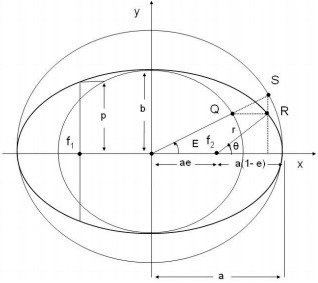
\includegraphics[width=(0.9\textwidth),height=(\textheight),keepaspectratio]{ellipse}
\caption{Ellisse.}
\end{figure}

\clearpage


\subsection{Parabola}

\begin{figure}[!ht]
\centering
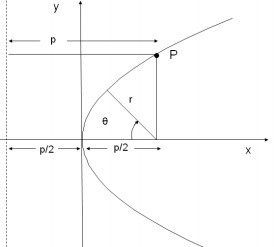
\includegraphics[width=(0.9\textwidth),height=(\textheight),keepaspectratio]{parable}
\caption{Parabola.}
\end{figure}

\begin{align*}
&r=\frac{p}{1+\cos{\theta}}\\
&y^2=2px
\end{align*}

\clearpage

\subsection{Iperbole}

\begin{figure}[!ht]
\centering
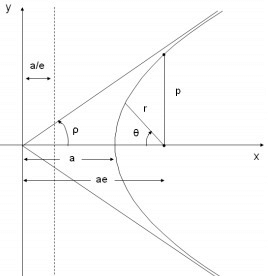
\includegraphics[width=(0.9\textwidth),height=(\textheight),keepaspectratio]{hyperbola}
\caption{Iperbole.}
\end{figure}

\begin{align*}
&\frac{x^2}{a^2}-\frac{y^2}{b^2}=1\\
&r=\frac{p}{1+e\cos{\theta}}\\
&e=\sqrt{1+\frac{b^2}{a^2}},\ p=a(e^2-1)\\
&x=a\cosh{F},\ y=b\sinh{F}
\end{align*}

\clearpage

\chapter{Equazioni differenziali}
\PartialToc

\section{Equazione di Poisson}

\subsection{Potenziale gravitazionale}

U \'e il potenziale gravitazionale, energia potenziale per unit\'a di massa.

\begin{align*}
&\nabla^2U=4\pi\rho G&\intertext{la soluzione \'e:}\\
&U(\vec{r})=-G\int\,d^3r\frac{\rho(r')}{|\vec{r}-\vec{r}'|}\\
\end{align*}

Infatti le soluzioni dell'equazione di Poisson generica \mblock{\Laplace \phi=f} si trovano a partire dalle soluzioni dell'equazione di Laplace \mblock{\Laplace\phi=0}:

\begin{align*}
&\Phi(\vec{x})=\left\{\begin{array}{c}-\frac{1}{2\pi}\log{|\vec{x}|}\ (n=2)\\
\frac{1}{n(n-2)\alpha(n)|\vec{x}|\expy{n-2}}\ (n\geq3)
\end{array}\right.&\intertext{soluzione dell'equazione di Poisson \'e}\\
&u(\vec{x})=\int_{R^n}\Phi(\vec{x}-\vec{y})f(\vec{y})\,d^ny
\end{align*}

Soluzione in 3D \'e
\begin{equation*}
\phi(\vec{x})=-\frac{1}{4\pi}\int_V\frac{f(\vec{x}'}{|\vec{x}-\vec{x}'|}\,d^3x'
\end{equation*}


\chapter{Integrali - Tecniche d'integrazione.}
\PartialToc

 
\section{Gaussian}
 
\subsection{Equazione di Saha: somma su tutti i momenti finali dell'elettrone}
\begin{align*}
&\frac{n_{r+1}}{n_r}=\frac{g_{r+1}}{g_r}\frac{8\pi}{n_eh^3}\exp{-\frac{\chi_r}{KT}}\int_0^{+\infty}p_e^2\exp{-\frac{p_e^2}{2m_eKT}}\,dp_e&\intertext{con $a^2=\frac{1}{2m_eKT}$ }\\
&\int_0^{+\infty}x^2\exp{-a^2x^2}\,dx=\frac{\sqrt{\pi}}{4a^3}
\end{align*}



\section{Step integral of Lane-Emden equation}
 
 I use the Lane-Emden eqution in the form
 \begin{equation*}
 \frac{d^2w}{dz^2}=-[\frac{2}{z}\frac{dw}{dz}]-w^n
 \end{equation*}
 
 Stepping outward in radius from the center $w_{i+1}$ is given by previous $w_i$ plus amount the density changes by over the step
 \begin{align*}
 &w_{i+1}=w_i+\Delta z(\frac{dw}{dz})_{i+1}&\intertext{the rate of changes of density with radius is unknown but I can write it in term of second derivative:}\\
 &(\frac{dw}{dz})_{i+1}=(\frac{dw}{dz})_i+\Delta z\frac{d^2w}{dz^2}&\intertext{e sostituendo l'espressione per la derivata seconda data dall'equazione di Lane-Emden ho:}\\
 &(\frac{dw}{dz})_{i+1}=(\frac{dw}{dz})_i-[\frac{2}{z_i}(\frac{dw}{dz})_i+w_i^n]\Delta z
 \end{align*}
 
 Starting at center where
 \begin{align*}
 &\frac{dw}{dz}|_0=0\\
 &w(0)=1
 \end{align*}
I determine $(\frac{dw}{dz})_{i+1}$ and then $w_{i+1}$.
 
 
\chapter{Corpi autogravitanti in equilibrio}
\PartialToc


\section{Corpi in rotazione: modello di fluido autogravitante.}
 
\subsection{McLaurin spheroids}

The shape of McLaurin spheroid is described by eccentricity
\begin{equation*}
e^2=\frac{a^2-b^2}{a^2}
\end{equation*}
where a and b are the major and minor half-axes of meridional cross-section.
 
\subsection{Accelerazione di gravit\'a}

Formule di McLaurin
\begin{align*}
&g_{eq}=2\pi G\rho a \frac{\sqrt{1-e^2}}{e^3}[\arcsin{e}-e\sqrt{1-e^2}]\\
&g_{eq}=4\pi G\rho a \frac{\sqrt{1-e^2}}{e^3}[e-\sqrt{1-e^2}\arcsin{e}]
\end{align*}

 
\chapter{Gas di Fermi degenere (elettroni)}
\PartialToc


\section{Gas di elettroni degenere per velocit\'a relativistiche}
 
\subsection{Variabili adimensionali}

\begin{align*}
\xi=\frac{p}{m_ec}\\
x=\frac{p_F}{m_ec}
\end{align*} 

\subsection{Pressione}
 
 \begin{align*}
 &P=\frac{8\pi c}{3h^3}\int_0^{p_F}p^3\frac{p/(mc)}{\sqrt{1+p^2/(mc)^2}}\,dp\\
 &=\frac{8\pi c^5m^4}{3h^3}\int_0^x\frac{\xi^4}{\sqrt{1+\xi^2}}\,d\xi\\
 &\int_0^x\frac{\xi^4}{\sqrt{1+\xi^2}}\,d\xi\\
 &=\frac{1}{8}[x(2x^2-3)\sqrt{1+x^2}+3\arcsinh{x}]
 \end{align*}
 
quindi riscrivo

\begin{align*}
&P=\frac{\pi m^4c^5}{3h^3}f(x)\\
&f(x)=[x(2x^2-3)\sqrt{1+x^2}+3\arcsinh{x}]\\
&=[x(2x^2-3)\sqrt{1+x^2}+3\ln{(x+\sqrt{1+x^2})}
\end{align*}

\subsection{Energia interna}

\begin{align*}
&U=\int_0^{p_F}f(p)E(p)\,dp=\frac{8\pi}{h^3}\int_0^{p_F}E(p)p^2\,dp&\intertext{esplicitando la dipendenza dell'energia \mblock{E=E_{T}-mc^2} ottengo}
&U=\frac{\pi m^4c^5}{3h^3}g(x)\\
&g(x)=8x^3[\sqrt{x^2+1}-1]-f(x)
\end{align*}

\section{Casi limite}

\subsection{Importance of relativistic effect: parametro x.}

\begin{align*}
&x=\frac{p_F}{mc}=\frac{v_F/c}{\sqrt{1-(v_F/c)^2}}\\
&\frac{v_F^2}{c^2}=\frac{x^2}{1+x^2}
\end{align*}

Se $x\ll1$ gli elettroni hanno velocit\'a non relativistiche; nel caso $x\gg1$ $\frac{v_F}{c}\approx1$.

\subsection{Espressioni asintotiche per $f(x)$ e $g(x)$: caso non relativistico ($x\to0$).}

\begin{align*}
&f(x)\abc{x\to0}\frac{8}{5}x^5\\
&g(x)\abc{x\to0}\frac{12}{5}x^5
\end{align*}

\subsection{Espressioni asintotiche per $f(x)$ e $g(x)$: caso ultra relativistico ($x\to\infty$).}

\begin{align*}
&f(x)\abc{x\to\infty}2x^4\\
&g(x)\abc{x\to\infty}6x^4
\end{align*}

\part{Physical Background}


\chapter{Relativity}
\PartialToc

\section{Kinematic}

\begin{align*}
&p=\frac{m_ev}{\sqrt{1-v^2/c^2}}\\
&E_{tot}=\frac{m_ec^2}{\sqrt{1-v^2/c^2}}=m_ec^2\sqrt{1+\frac{p^2}{m_e^2c^2}}\\
&E_k=\sqrt{p^2c^2+m^2c^4}-mc^2\\
&pc\ll mc^2:\ E_k\to\frac{p^2}{2m}\\
&pc\gg mc^2:\ E_k\to pc
\end{align*}


\chapter{Dynamic of fluids. MHD equations.}
\PartialToc

\section{Vectorial and upper order identity}

\begin{align*}
&\nabla\cdot(\vec{v}\cdot\ten{P})=\vec{v}\cdot(\nabla\cdot\ten{P})+\ten{P}:(\nabla\vec{v})\\
&\ten{A}:\ten{B}=\trace{A*B^T}
\end{align*}

\section{Dynamic equilibrium}

When there is motion we have a dynamical equilibrium and we have to add inertial term to hydrostatic condition (equilibrium is referred to comoving frame with fluid).

\subsection{Acceleration in fluid with spherical symmetry}

\begin{align*}
&\frac{v(r+v\,dt,t+dt)-v(r,t)}{dt}\to\TDof{t}v\\
&=\PDy{t}{v}+v\PDy{r}{v}&\intertext{Acceleration results from change in the velocity field at given place and the change due to the fact that fluid element moves. The first term is Eulerian variation, the whole is Lagrangian derivative. More generaly Lagrangian derivative defines the rate of change along with moving fluid $\downarrow$}\\
&\TDof{t}=\PDof{t}+\scap{v}{\nabla}
\end{align*}

\subsection{Eulerian description}

In Eulerian description all physical properties of fluid ($\vec{v}$, P $\rho$, T, etc) are regarded as field quantities depending on $(\vec{r},t)$ where $\vec{r}$ is the position of point of observation.

\subsection{Lagrangian description}

Motion of a given fluid element is followed: $\vec{r}$ denotes position of a given element depending on t and in general in 3D space on 3 parameter, if the are the component of the vector which was identical to $\vec{r}$ at say $t=0$ we have $\vec{r}(\vec{a},t)$ where $\vec{r}(\vec{a},0)=\vec{a}$.

Lagrangian description is used in 1D problem where a may represent T or interior mass.

\subsection{Material derivative}

Using the Lagrangian position variable we have 
\begin{align*}
&\dvec{r}=\TDy{t}{\vec{r}}=\vec{v}(\vec{r},t)\\
&\TDof{t}=\PDof{t}+\scap{v}{\nabla}
\end{align*}


\subsection{Equilibrium condition}

\begin{align*}
&\TDy{r}{P}+G\frac{m(r)\rho(r)}{r^2}=0&\intertext{alla condizione di equilibrio idrostatico aggiungo il termine dovuto all'accelerazione $\rho\TDy{t}{v}$ nel riferimento solidale all'elemento di fluido:}\\
&\rho(\PDy{t}{v}+v\PDy{r}{v})+\PDy{r}{P}+\frac{Gm(r)}{r^2}\rho=0&\intertext{vedi conservazione del momento}
\end{align*}

\subsection{Stationary flow. Bernoulli's equation: barotropic regime.}
It show how velocity of flow is affected by gravity and changes in density
\begin{align*}
&\rho(v\PDy{r}{v})+\PDy{r}{P}+\frac{Gm(r)}{r^2}\rho=0&\intertext{in stationary flow $v$ is function of r alone. In barotropic regime  $P(\rho)$ and $\uparrow$ integrates to }\\
&\frac{v^2}{2}+F(\rho)-\frac{GM}{r}=const&\intertext{$\uparrow$ Bernoulli's equation.}\\
&\rho\,dF=dP=c_s^2\,d\rho
\end{align*}

For a perfect adiabatic gas $F=\frac{\gamma}{\gamma-1}\frac{P}{\rho}$ and Bernoulli's equation become

\begin{align*}
&\frac{v^2}{2}+\frac{c_s^2}{\gamma-1}-\frac{GM}{r}=\frac{v_0^2}{2}+\frac{c_{s0}^2}{\gamma-1}-\frac{GM}{r_0}&\intertext{In the isothermal regime the sound speed is a constant:}\\
&\gamma\to1,\quad c_s^2=\TDy{\rho}{P}
\end{align*}

\section{Leggi di conservazione}

In astrophysical context $\vec{f}$ the force per unit mass is denoted by $\vec{g}$ the gravitational acceleration.

\subsection{Mass conservation}

A shell $[r,r+dr]$ contains mass $4\pi r^2\rho\,dr$: in infinitesimal time $dt$ a particle moves by $v(r,t\,dt)$ so

\begin{align*}
&r^2\to r^22rv\,dt\\
&dr\to dr+dr\PDy{r}{v}\,dt\\
&\rho\to\rho+(\PDy{t}{\rho}+v\PDy{r}{\rho})\,dt\\
\end{align*}

The total change in $r^2\rho\,dr$ must be zero
\begin{align*}
&2rv\rho+r^2(\PDy{t}{\rho}+v\PDy{r}{\rho})+r^2\rho\PDy{r}{v}=\\
&\TDy{t}{\rho}+\rho\underbrace{(\PDy{r}{v}+\frac{2v}{r})}_{\div{v}=\div{(v\frac{\vec{r}}{r})}}=0&\intertext{In general case (when no sperical symmetry is assumed)}\\
&\TDy{t}{\rho}+\rho\scap{\nabla}{v}=\PDy{t}{\rho}+\nabla\cdot(\rho\vec{v})=0&\intertext{infatti la trasformazione subita da un elemento di fluido in tempo $dt$:}\\
&\vec{r}\to\vec{r}+\vec{v}\,dt&\intertext{ \'e associata alla trasformazione nell'elemento di volume infinitesimo}\\
&dV\to\,dV(1+dt\,\scap{\nabla}{v})\quad (\frac{d\ln{dV}}{dt}=\scap{\nabla}{v})&\intertext{quindi in un fluido incompressibile the velocity is free of divergence $\div{v}=0$.}
\end{align*}

\subsubsection{Mass conservation: Eulerian and Lagrangian descriptions.}

Nella descrizione Euleriana la conservazione della massa si esprime tramite l'equazione di continuit\'a:

\begin{align*}
&\PDy{t}{\rho}+\nabla\cdot(\rho\vec{v})=0&\intertext{$\rho\vec{v}$ is the current density of mass flow}\\
&\frac{1}{\rho}\TDy{t}{\rho}=-\scap{\nabla}{v}\\
&\frac{1}{V}\TDy{t}{V}=\scap{\nabla}{v}\\
&\TDof{t}(\rho\,d\tau)=\TDof{t}(dm)=0
\end{align*}

Nella descrizione Lagrangiana \'e conveniente considerare l'espressione per la posizione di ogni elemento di massa $\vec{r}=\vec{r}(\vec{a},t)$ come una trasformazione continua di variabili (dot stands for Stokes derivative)

\begin{align*}
&\rho(\vec{a},t)J(\vec{r}[\vec{a},t])=\rho_0=\rho(\vec{a},t=0)\\
&J(\vec{r}[\vec{a},t])=|\PDy{a_k}{x_j}|,\quad\Rightarrow\quad\dot{J}\\
&=J\sum_i\PDy{a_i}{v_i}=J\scap{\nabla}{v}&\intertext{quindi, segue il risultato analogo a quello nella descrizione Euleriana:}\\
&\frac{\dot{\rho}}{\rho}=-\scap{\nabla}{v}
\end{align*}

\subsection{Momentum conservation}

Per i fluidi la conservazione della quantit\'a di moto \'e in sostanza la seconda legge di Newton: l'equazione risultante \'e l'equazione del moto. Nella descrizione Euleriana

\begin{align*}
&\rho\TDy{t}{\vec{v}}=-\nabla\cdot\ten{P}+\rho\vec{f}&\intertext{$\vec{v}$ is the fluid velocity (momentum per unit mass) and $\vec{f}$ is the total body or external force per unit mass and $\ten{P}$ is pressure tensor (symmetric for angular momentum conservation). Considero il caso di un corpo autogravitante:}\\
&\rho\TDy{t}{\vec{v}}+\nabla P+\rho\nabla U=\rho(\PDy{t}{\vec{v}}+\vec{v}\cdot\nabla\vec{v})\\
&+\nabla P+\rho\nabla U=0&\intertext{U is the gravitational potential energy per unit mass. Without $\rho\nabla U$ $\uparrow$ \'e l'equazione di Eulero.}
\end{align*}

The equation of motion may also be written in a form that doesn't require mass conservation
\begin{align*}
&\PDy{t}{(\rho\vec{v})}+\nabla\cdot\underbrace{(\rho\vec{v}\vec{v}+\ten{P})}_{\parbox{1cm}{Momentum flux density}}=\rho\vec{f}&\intertext{In absence of external force the rate of decreases of momentum (of volume density $\rho\vec{v}$) in a fixed volume of the fluid is equal to net outward rate of flow of momentum of flux $(\rho\vec{v}\vec{v}+\ten{P})\cdot\hat{n}$.}
\end{align*}

If stresses reduce to pure hydrostatic pressure $\ten{P}=P*Id$: the force due to stresses acting on a surface $dS\hat{n}$ is $-P\hat{n}\,dS$ that is a force acting along inward normal

\begin{align*}
&\rho\TDy{t}{\vec{v}}=-\nabla P+\rho\vec{f}&\intertext{$\uparrow$ is assumed mass conservation.}\\
&\nabla P=\rho\vec{f}&\intertext{$\uparrow$ hydrostatic equilibrium in a static fluid $\vec{v}=0$.}\\
&\PDy{t}{(\rho\vec{v})}+\nabla\cdot(\rho\vec{v}\vec{v}+PI)=\rho\vec{f}&\intertext{$\uparrow$  mass conservation is NOT assumed.}
\end{align*}

When turbolence, viscosity or large-scale magnetic field are present their effects can be described in terms of a pressure tensor.

\subsection{Energy conservation}

\subsubsection{Mechanical energy}

\begin{align*}
&\TDof{t}(\frac{1}{2}v^2)=-\frac{1}{\rho}\vec{v}\cdot(\nabla\cdot\ten{P})+\scap{f}{v}&\intu{say that the rate of increse of the kinetic energy per unit mass is equal to the rate at which the pressure gradient and body forces are doing work on the unit mass. It's obtained from momentum equation in Eulerian form $\downarrow$ diveded by $\rho$ and reduced to scalar multiplying both sides by $\vec{v}$}\\
&\rho\TDy{t}{\vec{v}}=-\nabla\cdot\ten{P}+\rho\vec{f}
\end{align*}

We have an integral form: supposing $\vec{v}\cdot\ten{P}\cdot\,d\vec{S}$ is small ($\ten{P}$ small near the surface or ($\vec{v}\cdot\ten{P}$) is nearly perpendicular to $d\vec{S}$ as in steadly rotating star) and stresses reduce to pure pressure (and using mass conservation)
\begin{align*}
&\TDof{t}\int_M\frac{1}{2}v^2\,dm\\
&=\int_M[P\TDof{t}(\frac{1}{\rho})]\,dm+\int_M\scap{f}{v}\,fm&\intertext{the first integral on the right side of $\uparrow$ is sum over all mass elements in entire system of the rate of \mblock{P\,dV(V=\frac{1}{\rho})} work that the material in each such mass element is doing on its surroundings.}
\end{align*}

\subsubsection{Thermal and Mechanical energy}

Conservation of thermal and mechanical energy gives the rate of change of kinetic and internal energy of a unit mass of fluid as it moves about.

Sia E l'energia interna, $\vec{f}$ la risultante delle forze esterne, e $\TDy{t}{q}$ il bilancio di calore lungo la linea di flusso, tutti per unit\'a di massa: uso il princio di conservazione della massa.

\begin{align*}
&\TDof{t}(\frac{1}{2}v^2+E)=-\frac{1}{\rho}\nabla\cdot(\ten{P}\cdot\vec{v})+\scap{f}{v}+\TDy{t}{q}&\intertext{l'equazione di Bernulli \'e un caso particolare di $\uparrow$.}
\end{align*}

Se non uso la conservazione della massa
\begin{align*}
&\PDof{t}(\rho E+\frac{1}{2}\rho v^2)\\
&+\nabla\cdot(\rho E\vec{v}+\frac{1}{2}\rho v^2\vec{v}+\ten{P}\cdot\vec{v})=\\
&=\rho\scap{f}{v}+\rho\TDy{t}{q}\\
\end{align*}

The quantity in parentheses is the energy flux vector
\begin{equation*}
\vec{j}_E=(\rho E\vec{v}+\frac{1}{2}\rho v^2\vec{v}+\ten{P}\cdot\vec{v})
\end{equation*}
\index{energy flux vector}
since in absence of external forces $\vec{f}=0$ and of heat gains or losses $\TDy{t}{q}=0$ the rate of decreses of sum of internal and kinetic energy (of volume density $\rho E+\frac{1}{2}\rho v^2$) in a fixed volume is equal to total outward rate of flux of energy across the surface bounding fixed volume $\oint_S\,d\vec{S}=\vec{j}_E$. If stresses reduce to hydrostatic pressure
\begin{align*}
&\vec{j}_E=\rho\vec{v}(\frac{1}{2}v^2+E+\frac{P}{\rho})&\intertext{$E+\frac{P}{\rho}$ is the enthalpy per unit mass.}
\end{align*}

\subsubsection{Thermal energy alone}

Generalized form of first principle of TD: dalla conservazione dell'energia meccanica e della somma dell'energia meccanica e termica segue
\begin{align*}
&\TDy{t}{E}=-\frac{1}{\rho}\ten{P}:(\nabla\vec{v})+\TDy{t}{q}&\intertext{if stresses reduce to pure pressures:}\\
&\TDy{t}{q}=\TDy{t}{E}+P\TDof{t}(\frac{1}{\rho})=\TDy{t}{E}+P\TDy{t}{V}\label{eq:Eintconservation}
\end{align*}

\subsection{Internal Energy conservation, constant composition, equation of states and adibatic exponent}

For astrophysical purpose 3 equivalent form of internal energy conservation are useful. The adiabatic exponents measure the response of system to adiabatic changes

Con le ipotesi aggiuntive che la composizione chimica sia costante, che la pressione sia determinata da una funzione di stato determinata da una coppia di variabili termodinamiche tipo $P(\rho,T)$ e analogamente per energia interna $E(\rho,T)$:

\begin{align*}
&\TDy{t}{\ln{P}}=\Gamma_1\TDy{t}{\ln{\rho}}+\frac{\rho(\Gamma_3-1)}{P}\TDy{t}{q}\\
&(=\Gamma_1\TDy{t}{\ln{\rho}}+\frac{\chi_T}{c_VT}\TDy{t}{q})\\
&\TDy{t}{\ln{T}}=(\Gamma_3-1)\TDy{t}{\ln{\rho}}+\frac{1}{c_VT}\TDy{t}{q}\\
&\TDy{t}{\ln{T}}=\frac{\Gamma_2-1}{\Gamma_2}\TDy{t}{\ln{P}}+\frac{1}{c_PT}\TDy{t}{q}&\intertext{$c_V$ e $c_P$ sono i colari specivici per unit\'a di massa, }\\
&\chi_T=(\PDly{T}{P})_{\rho},\quad \chi_{\rho}=(\PDly{\rho}{P})_{T}&\intertext{gli esponenti adiabatici}\\
&\Gamma_1=(\TDly{\rho}{P})_{Ad},\ \Gamma_3-1=(\TDly{\rho}{T})_{Ad},\\ &\frac{\Gamma_2-1}{\Gamma_2}=(\TDly{P}{T})_{Ad}=\frac{\Gamma_3-1}{\Gamma_1}&\intertext{da cui seguono le relazioni:}\\
&\Gamma_1=\chi_{\rho}+\chi_T(\Gamma_3-1),\\ &\gamma=\frac{c_P}{c_V}=\frac{\Gamma_1}{\chi_{\rho}},\ \Gamma_3-1=\frac{P\chi_T}{\rho c_VT}&\intertext{la terza di $\uparrow$ \' equivalente alla cos\'i detta relazione di reciprocit\'a}\\
&(\PDly{\rho}{E})_T=\frac{P}{\rho E}(1-\chi_T)&\intertext{Vedi Landau statistical Physics intorno al $\S16$.}
\end{align*}

La condizione che la pressione sia definita dalla funzione termodinamica equivale a trascurare la viscosit\'a radiativa e molecolare, i campi magnetici su larga scala e le turbolenze.


\section{Transport}

\subsection{scalar quantity}

The mean free path of a particle is $l_c$: if Q depends only on z we consider two surfaces at $z-\frac{l_c}{2}$ and $z+\frac{l_c}{2}$.

\begin{align*}
&Q(z+\frac{l_c}{2})-Q(z-\frac{l_c}{2})\approx l_c\PDy{z}{Q}&\intu{net quantity of Q transfered (collisional processes), and vice versa.}\\
&F_Q=nv_T[Q(z-\frac{l_c}{2})-Q(z+\frac{l_c}{2})]\\
&\approx-nv_Tl_c\PDy{z}{Q}\\
&\vec{F}_Q=-nv_Tl_c\nabla Q&\intu{$l_c$ gives order of magnitude: precise numerical coefficient have to take in account for velocity distribution.}\\
&\TDof{t}\int_V\,dVQ=-\int_S\,dS\scap{n}{F_Q}\\
&=-\int_V\,dV\scap{\nabla}{F}_Q&\intu{no sources in the volume}\\
&\rho\TDy{t}{Q}=\nabla\cdot(\rho v_Tl_C\nabla Q)&\intertext{mass is conserved so Lagrangian derivative of $\rho\,dV$ vanishes.}
\end{align*}

\subsection{Heat}

\begin{align*}
&Q=c_PT&\intu{thermal energy per unit mass}\\
&\chi=v_Tl_C&\intu{heat flows to the cooler parts: heat transport coefficient or heat diffusivity}\\
&\rho\TDy{t}{Q}=\nabla\cdot(\rho\chi\nabla (c_PT))+S&\intu{heat transport equation S is a source or sink: production rate per unit volume}\\
&\rho c_P\TDy{t}{T}=\kappa \nabla^2T+S&\intu{$\kappa=\rho\chi c_P$, $\rho$, $\chi$, $c_P$ are constant.}\\
\end{align*}

The heat transport equation  must be supplemented with boundary conditions at surface (radiative loss) and continuity condition across sharp transition (in planets: core mantle): with energy source at the transition (with dimension of flux) we expect a jump in the flux $\rho\chi\hat{n}\cdot\nabla(c_PT)$ so $\mvar{}[\rho\chi\hat{n}\cdot\nabla(c_PT)]=F$.

If $T(z,t)$ is the only variable and fluid is at rest
\begin{align*}
&\PDy{t}{T}=\chi\PtwoDy{z}{T}&\intu{parabolic equation. An initial spike spreads after time t over distance $\sqrt{\chi t}$ and there is no wave propagation}\\
&T(z,t)=\frac{K}{2\sqrt{\pi\chi t}}\exp{-\frac{z^2}{4\chi t}}\\
&\lim_{t\to0}T(z,t)=K\delta(z)&\intertext{total thermal energy is conserved $\propto\int\,dz T=K$}
\end{align*}

\subsection{Momentum: viscosity.}

\begin{align*}
&Q=m_{mol}v_x(z)&\intertext{the sheared velocity field is smoothed out}\\
&\eta=\rho v_Tl_C&\intu{viscosity coefficient}\\
&\rho(\PDy{t}{\vec{v}}+\vec{v}\cdot\nabla\vec{v})+\nabla P+\rho\nabla U\\
&=\eta[\nabla^2\vec{v}+\frac{1}{3}\nabla(\scap{\nabla}{v})]&\intd{for incompressible flow $\scap{\nabla}{v}=0$ becomes}\\
&\rho(\PDy{t}{\vec{v}}+\vec{v}\cdot\nabla\vec{v})+\nabla P+\rho\nabla U=\eta\nabla^2\vec{v}&\intu{Navier-Stokes equation, $\eta/\rho$ is the kinematic viscosity.}
\end{align*}

Viscosity results in dissipation, the kinetic energy of the fluid motion is transformed into heat and should be accounted for in heat transfer equation
\begin{align*}
&E{Kin}=\frac{1}{2}\int\,dV\rho v^2\\
&\TDy{t}{E{Kin}}=-\frac{1}{2}\int\,dVq_{ij}(\PDy{r_j}{v_i}+\PDy{r_i}{v_j})&\intertext{$q_{ij}$ is the viscous stress tensor depending on velocity and its derivatives respect spatial coordinates}\\
&\TDy{t}{E{Kin}}=-\frac{\eta}{2}\int\,dV(\PDy{r_j}{v_i}+\PDy{r_i}{v_j})^2
\end{align*}

The relevance of viscosity is described by Reynold number\index{Reynold number} 
\begin{align*}
Re=\frac{\rho Lv}{\eta}&\intertext{L is a macroscopic characteristic length, v is a typical velocity of the flow}
\end{align*}


\section{Partially/totally ionized gas.}

At sufficient high temperatures and low densities (possibly under strong UV radiation from the sun) the gas may becomes partially or totally ionized. When the number of particles in square cube $\lambda_D$ is large and for scales larger than $\lambda_D$ approximate charge neutrality holds and we can describe the gas as a single neutral fluid.

Relative motions of electrons and ions produce electric currents and magnetic fields.

Astrophysical fluids are at least partially ionized  thus electromagnetic forces can be more important for macroscopic dynamics: Magneto-hydrodynamics is the name used when we deal with continuum mechanics for charged matter otherwise plasma physics.

\section{Maxwell's equations}

At microscopic level the field $\vec{E},\vec{B}$ are determined by charge densities $\sigma_c$ and current densities $\vec{J}$
\begin{align*}
&\scap{\nabla}{E}=4\pi\rho_c\\
&\vecp{\nabla}{B}-\frac{1}{c}\PDy{t}{\vec{E}}=\frac{4\pi}{c}\vec{J}&\intertext{Gaussian Units}
\end{align*}

and Faraday's law, absence of magnetic monopoles

\begin{align*}
&\vecp{\nabla}{B}+\frac{1}{c}\PDy{t}{\vec{B}}=0\\
&\scap{\nabla}{B}=0
\end{align*}

An arbitrary EM field tha fulfils the continuity equation
\begin{equation*}
\PDy{t}{\rho_c}+\scap{\nabla}{J}=0
\end{equation*}
can be propagated in time.

At macroscopic level in presence of matter the electric field is affected also by polarization and similarly magnetic fields
\begin{align*}
&\scap{\nabla}{D}=4\pi\rho_c\\
&\vecp{\nabla}{H}-\frac{1}{c}\PDy{t}{\vec{D}}=\frac{4\pi}{c}\vec{J}\\
&\vecp{\nabla}{B}+\frac{1}{c}\PDy{t}{\vec{B}}=0\\
&\scap{\nabla}{B}=0&\intertext{Gaussian Units}
\end{align*}

We need constitutive relations between $\vec{B}$, $\vec{H}$ and $\vec{E}$, $\vec{D}$: when fields are weak and matter isotropic
\begin{align*}
&\vec{B}=\mu\vec{H}\\
&\vec{D}=\epsilon\vec{E}
\end{align*}
In normal modes of oscillation the electric and magnetic response depends on the mode: the constitutive equations are expressed in term of Fourier component of the field.

\section{Magneto-hydrodynamics}

\subsection{Equation for boh fluid}

The equation of motion (confronta con cox, bertotti, Dalsgaard\index{da fare: eq moto})

\begin{align*}
&\rho\PDy{t}{\vec{v}}+\nabla P+\rho\nabla U\\
&=\rho(\PDy{t}{\vec{v}}+\scap{v}{\nabla\vec{v}})+\nabla P+\rho\nabla U=0&\intertext{without the term $\rho\nabla U$ is called the Euler equation}
\end{align*}

\subsection{Electrically conductive fluid}

In a moving conductor Ohm's law must be modified
\begin{align*}
&\vec{J}=\sigma(\vec{E}+\frac{1}{c}\vecp{v}{B})&\intertext{In presence of factor that destroy the isotropy of the fluid the conductivity is a tensor. When the conductivity is large enough that we can replace the equation $\uparrow$ with:}\\
&\vec{E}+\frac{1}{c}\vecp{v}{B}=0
\end{align*}

In electrically conductive fluid the magnetic force must be added to EOM. A charge q moving with velocity $\vec{u}$ in a magnetic field $\vec{B}$ suffers a Lorentz force $\frac{q}{c}\vecp{u}{B}$: for all charged particles in an infinitesimal volume we get $\sum q\vecp{u}{B}=\vecp{J}{B}\,dV$. Aggiungo il contributo della forza di Lorentz per unit\'a di volume all'equazione di conservazione della quantit\'a di moto:
\begin{equation*}
\rho\TDy{t}{\vec{v}}+\nabla P+\rho\nabla U=\frac{1}{c}\vecp{J}{B}
\end{equation*}

La pressione deve essere espressa in funzione della densit\'a o direttamente tramite una dipendenza politropica o indirettamente tramite l'equazione di stato e del bilancio energetico.

Since electric and magnetic fields are created by motions of fluid at speed $v\ll c$: their time and space variations are related by \mblock{\PDof{t}\approx v\nabla\ll c\nabla} and we have the Ampere law in simpler form neglecting displacement current
\begin{align*}
&c\vecp{\nabla}{B}=4\pi\vec{J}&\intertext{$\uparrow$ current density is solenoidal and net charges are neglected. This is in agreement with general property of plasma in which there are no charge fluctuations in volumes much larger than $\lambda_D$. The small charge density can be recovered taking the divergence of Ohm's law $\downarrow$}\\
&\vec{J}=\sigma(\vec{E}+\frac{1}{c}\vecp{v}{B})
\end{align*}

This approcimation cannot deal with electromagnetic waves for wich E and B are of same order of magnitude.

\subsection{Magnetic stress tensor}

Scrivo la forza magnetica per unit\'a di volume

\begin{align*}
&\vec{f}=\frac{1}{c}\vecp{J}{B}+\div{-\frac{B^2}{8\pi}\ten{1}+\frac{\ten{B}}{4\pi}}\\
&=\div{\ten{{P^M}}}&\intertext{$\uparrow$ ho usato espressione}\\
&(\nabla\wedge\vec{B})\wedge\vec{B}
\end{align*}
\index{(C) espressione magnetic stress tensor}
Let's illustrate the signifiance of magnetic stress tensor with two examples:

\begin{itemize*}
\item Magnetic field along z but with arbitrary intensity $B(x,y)$.

$\ten{{P^M}}$ is a scalar and a flow in $(x,y)$ plane is governed by total pressure

\begin{align*}
&P+\frac{B^2}{8\pi}&\intertext{where the latter term $\frac{B^2}{8\pi}$ is the magnetic pressure that has the effect of pushing the flow away from high intensity regions.}
\end{align*}

This happens , ie, in the interaction between supersonic solar wind and Earth's dipole field which acts like an obstacle with the magnetic pressure giving rise to a shock front.

The magnetic pressure prevail over the fluid pressure P when the ratio $\beta=\frac{8\pi P}{B^2}$ is small.

\item B has uniform intensity but its direction $\hat{n}$ is not.

Only potive component along $\hat{n}\hat{n}$ is relevant

Transversal waves with Alfv\'en speed 

\begin{align*}
&V_A=\sqrt{\frac{B^2}{4\pi\rho}}
\end{align*}

\end{itemize*}

\section{The induction equation. Magnetic diffusion coefficient}

\subsection{Induction equation}

When conductivity $\sigma$ is constant
\begin{align*}
&\PDy{t}{\vec{B}}=\nabla\wedge(\vec{v}\wedge\vec{B})+\frac{c^2}{4\pi\sigma}\nabla^2\vec{B}\\
&\lambda=\frac{c^2}{4\pi\sigma}&\intertext{$\uparrow$ is the magnetic diffusion coefficient. The analog of viscosity. In a medium at rest ($\vec{v}=0$) the induction equation is equivalent to heat equation with conductivity $\lambda$: an initial magnetic field spike after a time t spread over a distance $c\sqrt{\lambda t}$.}
\end{align*}
 
\subsection{Infinite conductivity limit}

In a perfectly conductive fluid holds
\begin{align*}
&\vec{E}+\frac{1}{c}\vec{v}\wedge\vec{B}=0&\intertext{contrary to Newtonian dynamics in this case the electromagnetic field determines the component of the velocity orthogonal to the line of force not its time derivative}\\
&\vec{v}_{\perp}=c\frac{\vecp{E}{B}}{B^2}
\end{align*}
La componente lungo $\vec{B}$ della velocit\'a obbedisce all'equazione della conservazione dell'impulso. Dalla legge di Ohm risulta che il campo elettrico e magnetico sono ortogonali, il campo elettrico lungo le linee di forza \'e annullato dal moto delle cariche. 

\subsection{MHD equation: infinite conductivity, no gravity, no viscosity.}

\begin{align*}
&\rho[\PDy{t}{\vec{v}}+(\scap{v}{\nabla})\vec{v}]+\nabla P=\frac{1}{4\pi}(\nabla\wedge\vec{B})\wedge\vec{B}\\
&\PDy{t}{\rho}+\nabla\cdot(\rho\vec{v})=0\\
&\PDy{t}{\vec{B}}=\nabla\wedge(\vec{v}\wedge\vec{B})
\end{align*}


\section{Conservation of magnetism and vorticity (???).}

\subsection{Rate changes surface dragged along flux}

\begin{align*}
&\TDof{t}(d\vec{r})=(d\vec{r}\cdot\nabla)\vec{v}\\
&\TDof{t}(dS_i)=dS_i\scap{\nabla}{v}-dS_j\PDy{r^i}{v^j}\\
&dV=d\vec{S}\cdot\,d\vec{r}=\frac{dm}{\rho}
\end{align*}

\subsection{Conservation magnetic flux and circulation}

\begin{align*}
&\TDy{t}{\vec{B}}=\PDy{t}{\vec{B}}+(\scap{v}{\nabla})\vec{B}\\
&=(\scap{v}{\nabla})\vec{v}-\vec{B}(\scap{\nabla}{v})+\frac{c^2}{4\pi\sigma}\nabla^2\vec{B}&\intu{Lagrangian change in magnetic field}\\
&\TDof{t}(\vec{B}\cdot\,d\vec{S})=\frac{c^2}{4\pi\sigma}\,d\vec{S}\cdot\nabla^2\vec{B}&\intu{Lagrangian change in magnetic flux through $d\vec{S}$}
\end{align*}

\subsection{Frozen flux and freezing theorem}

When conductivity is infinite the flux through a surface attached to the fluid is constant and dragged along with the fluid (Alfv\'en's frozen flux theorem). In the collapse of a cosmic body of size R, B increases as $1/R^2$: this can produces large amplification of magnetic field. Similarly when a charged particle moves in a slowly varying magnetic field the flux embraced in a Larmor gyration remains almost constant.

Freezing theorem (cosmic physics/solar wind)
\begin{align*}
&\TDof{t}(d\vecp{r}{B})=-\vec{B}\wedge(\,d\scap{r}{\nabla})\vec{v}+\\
&+\,d\vec{r}\wedge[(\scap{B}{\nabla})\vec{v}-\vec{B}(\scap{\nabla}{v})]\\
&+\frac{c^2}{4\pi\sigma}\,d\vec{r}\wedge\nabla^2\vec{B}&\intertext{If initially $\vec{r}$ and $\vec{r}+d\vec{r}$ lie on same line of force so that $d\vecp{r}{B}=0$ ($d\vec{r}$ and $\vec{B}$ being parallel) then the first two terms on rhs of $\uparrow$ cancel each other.}
\end{align*}

In infinitely conductive plasma the condition $d\vecp{r}{B}=0$ holds forever: a line of force is tied to the fluid element lying on it.

\subsection{Kelvin vorticity theorem}
Negligible viscosity

\begin{align*}
&\TDof{t}\int_s\,d\vec{S}\cdot(\vecp{\nabla}{v})=0
\end{align*}

In a barotropic inviscid fluid the vorticity lines are anchored to the matter.


\chapter{Gravitational field}\label{chap:gravity}
\PartialToc

\section{Gravitational energy}

\subsection{Poisson's equation: superposition principle.}

$U$, energia potenziale gravitazionale per unit\'a di massa o potenziale gravitazionale, \'e soluzione dell'equazione di Poisson
\begin{equation*}
\nabla^2U=4\pi G\rho
\end{equation*}
quindi 
\begin{align*}
U(\vec{r})=-G\int d^3r'\frac{\rho(\vec{r}')}{|\vec{r}-\vec{r}'|}
\end{align*}

For a point mass M we have the monopole $U=-G\frac{M}{r}$. The linearity of poisson's equation ensure the superposition principle: the potential of N bodies is the sum of individual potentials.

\subsection{Gravitational acceleration}

We obtain the force per unit mass acting on the fluid from gravitational potential

\begin{align*}
&\vec{f}(\vec{r},t)=\vec{g}(\vec{r},t)=-\nabla U(\vec{r},t)\\
&\scap{\nabla}{f}=-4\pi G\rho
\end{align*}

\subsection{Energia gravitazionale.}
Considero massa unitaria a distanza r: l'energia potenziale dovuta a $m(r)$ \'e $-\frac{Gm(r)}{r}$. L'energia potenziale $E_g$ \'e la somma su tutti gli elementi $dm$ della stella e $-E_g>0$ \'e l'energia necessaria per espandere tutti i gusci a infinito. 

\begin{align*}
&E_g=-\int_0^M\frac{Gm(r)}{r}\,dm
\end{align*}

\section{Gravitional equilibrium}

L'equilibrio di una struttura su scala cosmica \'e determinato dall'equilibrio tra attrazione gravitazionale e pressione interna. La pressione interna \'e determinata dall ostato della materia, dalla composizione, il flusso di calore, il campo magetico, etc.

This factors are influenced by the way the body was formed and its history. Their determination require laws of microscopical physics: state of stress (pressure tensor) provides link between microscopical state and global structure. If as in fluids microscopic states have no privileged direction the pressure tensor depend only on the scalar pressure: deviation from spherical equilibrium will occur also if part of the body is solid capable of supporting tangential forces at its surface.

\section{Configurazione sferica}

\subsection{Gauss theorem}

The gravitational acceleration $\vec{g}$ produced by point mass $m$ is formally obtained from electrostatic field produced by charge $q$ substituting $q$ with $-Gm$.
\begin{align*}
&g(r)=G\frac{M(r)}{r^2}\\
&\int_S\,dS\scap{n}{g}=-4\pi GM(r)
\end{align*}

\subsection{Gravitational potential energy per unit of mass}

\begin{align*}
&\vec{g}=-\nabla U&\intertext{U is the gravitational potential energy per unit mass. Outside the mass:}\\
&U(r>R)=-\frac{GM}{r}\\
&U(r<R)=-G[4\pi\int_r^R\,drr\rho(r)+\frac{m(r)}{r}]&\intertext{$\uparrow$ inside a thin spherical shell of mass $dM$ the gravitational pull is $0$ so $U$ is constant and equal to its value just outside, \mblock{-g\frac{dM}{r}=-4\pi G\rho(r)r\,dr}, therefore the total value is the sum of shell outside r and those inside, $-G\frac{m(r)}{r}$.}
\end{align*}

\subsection{Gravitational binding energy}

\begin{align*}
&E_B=-\frac{1}{2}G\iint\frac{dm(\vec{r})dm(\vec{r'})}{|\vec{r}-\vec{r'}|}\\
&=2\pi\int_0^Rdr\,r^2\rho(r)U(r)
\end{align*}

\section{Deviazioni da simmetria sferica}

\subsection{Rotational deformations: Parametro di Helmert}

\begin{align*}
\mu_c=\frac{R^3\omega^2}{GM}&\intertext{$\uparrow$ ratio between rotational energy and gravitational binding energy: il parametro di Helmert.}
\end{align*}

\subsection{Oblateness}

Sulla superficie la deformazione \'e misurata dall'XXX

\begin{align*}
\epsilon=\frac{R_e-R_p}{R}\approx\mu_c
\end{align*}



\chapter{Statistical physics. Thermodynamics.}
\PartialToc


\section{Distribution functions}

The distribution function for a species of particle measures the density of that species in combined 6D phase space.

\subsection{Thermodynamical description is complete?}
In a rarefied medium we must question if the flow can be completely described with mean quantities $\rho$, $\vec{v}$, T (eventually $\vec{B}$).

\subsection{Thermodynamical equilibrium}

After few collision fluid is described by locally Maxwellian distribution function which depends on space and time only through n, $\vec{v}$, T
\begin{equation*}
f=n(\frac{m}{2\pi kT})\expy{\frac{3}{2}}\exp{-\frac{m|\vec{u}-\vec{v}|^2}{2kT}}
\end{equation*}

Collision occur at rate $\nu_c=n\exv{u\sigma_c}$ (collision frequency)\index{collision frequency} averaging cross sections with velocity distributions. The gas is brought into a local thermodynamical equilibrium and is described by a fluid model. Conservation laws provide time evolution for averaged quantities. After this if the system closed and isolated on space scale L and time scale $\frac{L^2}{v_Tl_c}$ it will be brought into uniform state ~\ref{eq:uniformstate} by diffusion and dissipative processes. For lo0cal thermodynamical equilibrium typical scales for macroscopic variation in time and space by external agents must be much larger than $\frac{1}{\nu_c}$ and mean free path $l_c=\frac{v_T}{\nu_c}$ resp.

\section{Thermodynamical potential}

\subsection{Funzione termica: entalpia.}

\begin{equation*}
H=E+PV
\end{equation*}

\subsection{Entropia}

\begin{align*}
ds=\frac{dq}{T}=\frac{1}{T}[(\PDy{v}{u})_T+P]\,dv+\frac{1}{T}(\PDy{T}{u})_v\,dT
\end{align*}

\subsection{Energia libera F.}

Il lavoro corrispondente ad una variazione isotermica reversibile infinitesima dello stato del corpo si pu\'o scrivere come differenziale di una certa grandezza $F$

\begin{align*}
&dU-dQ=dU-T\,dS=d(U-TS)\\
&dF=dU-T\,dS-S\,dT\\
&dq=T\,dS=dU+P\,dV\\
&dF=-S\,dT-P\,dV
\end{align*}

\subsection{Potenziale termodinamico G}

\begin{align*}
&dG=dF+P\,dV+V\,dP\\
&dG=-S\,dT+V\,dP
\end{align*}

\subsection{Dipendenza delle grandezze termodinamiche dal numero di particelle}

\begin{align*}
&U=Nf(\frac{S}{N},\frac{V}{N})\\
&F=Nf(\frac{V}{N},T)\\
&H=Nf(\frac{S}{N},P)\\
&G(=\Phi)=Nf(P,T)\\
&dH=T\,dS+V\,dP+\mu\,dN\\
&dF=-S\,dT-P\,dV+\mu\,dN\\
&dG(=d\Phi)=-S\,dT+V\,dP+\mu\,dN\\
&\mu=\Dcvar{\PDy{N}{H}}{S,P}=\Dcvar{\PDy{N}{F}}{T,V}=\Dcvar{\PDy{N}{\Phi}}{P,T}
\end{align*}

Introduco la densit\'a numerica (specifica) $N_i=\frac{n_i}{\rho}$ (particelle per grammi): lagrangian version of $n_i$ (remain constant if volume changes).

\begin{definition}{Potenziale chimico}
Il potenziale chimico \'e definito da
\begin{equation*}
\mu_i=\Dcvar{\PDy{N_1}{E}}{S,V}
\end{equation*}
Not to be confused with molecular weight.
\end{definition}

Thermodynamical equilibrium requires \mblock{\sum_i\mu_i\,dN_i=0}.

Given $(T,\rho)$ and the possible reactions we are able to find all $N_i$ for a gas in thermodynamical equilibrium: informations about $N_i$ is contained in $\mu_i$ for given $(T,\rho)$.

\subsection{Occupation number for perfect gas.}

Distribution function for the species
\begin{align*}
&n(p)=\frac{1}{h^3}\sum_j\frac{g_j}{\expp{(\frac{-\mu+E_j+E(p)}{kT})}\pm1}
\end{align*}
$\mu$ \'e il potenziale chimico delle varie specie, $j$ conta i possibili livelli energetici della specie, $g_j$ \'e la degenerazione del livello dello stato $j$, $E(p)$ \'e l'energia cinetica.

\begin{usefull}{Distribution function}
The distribution function $n(p)$ is in unit of: Particle per $(cm * \text{unit of momentum})^3$.

\end{usefull}


\subsection{Particles: Maxwell distro}

Collisions have time and space to produce local thermal Boltzmann distribution of velocities. Maxwellian distribution f in velocity space

\begin{usefull}{Maxwell distribution}

\begin{align}\label{eq:uniformstate}
&f=n(\frac{m}{2\pi kT})\expy{\frac{3}{2}}\exp{-\frac{mu^2}{2kT}}&\intertext{$f\,d^3r\,d^3u$ is the number of particles in the phase space volume element $d^3r\,d^3u$, $n=N/V$ is the number density}
\end{align}

\end{usefull}

\begin{usefull}{MB: most probable velocity. Averaged quantities}

\begin{align*}
&\TDy{v}{f}=0\\
&v_{prob.}=\sqrt{\frac{2kT}{m}}
\end{align*}

\begin{align*}
&n(\vec{r},t)=\int d^3u\,f(\vec{r},\vec{u},t)\\
&n(\vec{r},t)\vec{v}(\vec{r},t)=\int d^3u\,\vec{u}f(\vec{r},\vec{u},t)\\
&3n(\vec{r},t)kT(\vec{r},t)=m\int d^3u\,u^2f(\vec{r},\vec{u},t)\\
&=mnv_T^2\\
&v_T=\sqrt{\frac{kT}{3m}}&\intu{thermal speed}
\end{align*}

\end{usefull}



\subsection{Radiation: Planck distro}

The frenquency distribution is uniquely determined by temperature in terms of Plank's distribution function

\begin{align*}
&n_{\nu}\,d\nu\,dV=\frac{8\pi\nu^2}{c^3}\frac{d\nu\,dV}{\exp{\frac{h\nu}{kT}}-1}\\
&u_{\nu}=h\nu n_{\nu}&\intu{spectral energy density}\\
&u_{\nu}\propto\nu^2&\intu{for frequency much less than $kT/h$, that is in the Rayleigh limit:}\\
&u_{\nu}=\frac{8\pi kT}{c^3}\nu^2&\intu{Rayleigh-Jeans law.}\\
&\lambda_{Max}=\frac{b}{T},\quad b\approx0.290\si{\cm\kelvin}&\intu{Wien displacement law: wavelength at which spectral energy density has maximum.}\\
&u=\intzi\,d\nu u_{\nu}=aT^4&\intu{is finite}\\
&a=\frac{4\sigma}{c}\approx\num{7.56e-15}\si{\erg\per\cubic\cm\per\kelvin\tothe{4}}
\end{align*}


\section{Boltzmann's equation}

\subsection{Need for a closure relation}

From conservation equations we have 5 five lin. indip. relations (momentum: vectorial, energy: scalar, mass: scalar) and thirteen variables \mblock{\rho,\ u_i,\ P,\ \pi_{ik}\,(5)}.

Until we introduce a way to derive a closed set of moment equations everything has no real physical content.

\subsubsection{When we can find usefull closure relations?}

\begin{itemize}
\item Mean free path smaller than system scale length: \mblock{l\ll L}. we expect LTE for translational degrees of freedom to hold. The Chapman-Enskog procedure allow us to derive closure relations.

To zeroth-order in a systematic expansion for small $\frac{l}{L}$ we shall find that eight needed relations take the form \mblock{\pi_{ik}\approx0,\ F_i\approx0}: the neglect of diffusive effects leads to a complete set of fluid relations called Euler equations. The next order approximation are the Navier-Stokes equations in which diffusive terms \mblock{\pi_{ik},\ F_i} are not zero.

\item Mean free path much larger than system scale length, $l\gg L$: is the analogous of an optical thin system for radiative transfer but we cannot assume particle travel in straight lines because they are subjected to macroscopical large-scale forces that bend trajectories.

When collision are unimportant we have free-molecular flow (Knudsen regime) in which particles move indipendently of each others. When none of these two extreme approximations hold we study the deviations from Maxwell's distribution: a dynamical description in phase space must be adopted using differential equation for for particle distribution function f, the Boltzmann's equation.

\end{itemize}

\subsection{Higher order velocity moments of Boltzmann's equation}

Succesive approximation to the solution of Boltzmann's equation
\begin{align*}
&S=-k\int f\ln{f}\,d^3x\,d^3p&\intu{entropy of a thermally isolated gas}\\
&\begin{pmatrix}
\rho\\\rho\vec{u}\\\rho U\\
\end{pmatrix}
=\int\begin{pmatrix}
m\\m\vec{v}\\\frac{m}{2}|\vec{v}-\vec{u}|^2\\
\end{pmatrix}f(\vec{x},\vec{v},t)\,d^3v\\
&\PDy{t}{f}+\vec{v}\cdot\PDy{\vec{x}}{f}+\dvec{p}\cdot\PDy{\vec{p}}{f}=C(f)=\Dcvar{\frac{\delta f}{\delta t}}{coll}\\
&\Dcvar{\frac{\delta f}{\delta t}}{coll}=\int|\vec{v}-\vec{v}_2|\sigma(\Omega)*\\
&*[f(\vec{v}')f(\vec{v}_2')-f(\vec{v})f(\vec{v}_2)]\,d\Omega\,d^3v_2&\intu{Boltzmann's equation: we wish to derive equations governing spacetime evolution of $\rho$, $\vec{u}$, $U$. We multiply BE by \mblock{\chi(\vec{v}=\insieme{m,m\vec{v},m\vec{v}\vec{v}}}}\\
&\int(\chi\PDy{t}{f}+\chi v_k\PDy{x_k}{f}+\chi\dvec{p}\PDy{\vec{p}}{f})\,d^3v\\
&=\int\chi\Dcvar{\frac{\delta f}{\delta t}}{coll}\,d^3v
\end{align*}

The formal procedure consists of succesive approxs for solution of BE in limit of\mblock{\frac{l}{L}\ll1}.

Order of magnited estimate:

Source/sink part of \mblock{\Dcvar{\frac{\delta f}{\delta t}}{coll}\approx\nu_c f} where \mblock{\nu_c=n\exv{\sigma w}} is the collision frequency, the terms on left side of Boltzamnn's equation have order of mag. $\frac{uf}{L}$, if $u\approx w$ the ratio of terms one left side and right side is $\approx\epsilon$:
\begin{align*}
&L(f)=\epsilon\expy{-1}C(f|f)\\
&L=\PDof{t}+\vec{v}\PDof{\vec{x}}+\dvec{p}\PDof{\vec{v}}\\
&C(f|g)=\int|\vec{v}-\vec{v}_2|\sigma(\Omega)*\\
&*[f(\vec{v}')g(\vec{v}_2')-f(\vec{v})g(\vec{v}_2)]\,d\Omega\,d^3v_2
\end{align*}

We attempt a solution in form of series expansion
\begin{align*}
&f=f_0+\epsilon f_1+\epsilon^2f_2+\ldots\\
&\int\begin{pmatrix}
m\\m\vec{v}\\\frac{m}{2}|\vec{v}-\vec{u}|^2\\
\end{pmatrix}f_0\,d^3v=\begin{pmatrix}
\rho\\\rho\vec{u}\\\rho U\\
\end{pmatrix}\\
&\int\begin{pmatrix}
m\\m\vec{v}\\\frac{m}{2}|\vec{v}-\vec{u}|^2\\
\end{pmatrix}f_N\,d^3v=0
\end{align*}

\subsubsection{Euler equations}

Lowest order $C(f_0|f_0)=0$: \mblock{\ln{f_0}=am+\vec{b}m\vec{v}+c\frac{m}{2}|\vec{v}|^2}.
To the zeroth order:
\begin{align*}
&f_0=n(\frac{m}{2\pi kT})\expy{\frac{3}{2}}\exp{-\frac{m|\vec{v}-\vec{u}|^2}{2kT}}&\intu{implies constitutive relation:}\\
&\rho U=\frac{3}{2}P=\frac{3}{2}nkT\\
&\vec{w}=\vec{v}-\vec{u}\\
&\pi_{ik}^{(0)}=0,\ F_i^{(0)}=0&\intd{3 Euler equations:}\\
&\PDy{t}{\rho}+\nabla\cdot(\rho\vec{u})=0\\
&\PDy{t}{\vec{u}}+\nabla(\frac{1}{2}\vec{u}^2)+(\vecp{\nabla}{u})\wedge\vec{u}=\dvec{p}-\frac{1}{\rho}\nabla P\\
&((\scap{u}{\nabla})\vec{u}=\nabla(\frac{1}{2}\vec{u}^2)+(\vecp{\nabla}{u})\wedge\vec{u})\\
&\rho(\PDy{t}{U}+\vec{u}\cdot\nabla U)=-P\scap{\nabla}{u}\\
&s=c_v\ln{P\rho\expy{-\gamma}}&\intu{specific entropy of classic perfect gas}
\end{align*}

\subsubsection{Navier-Stokes equations}

To next order we find the solution in $f_1$ for \mblock{C(f_1|f_0)+C(f_0|f_1)=Lf_0}. In linear order approx:
\begin{align*}
&\pi_{ik}=\mu D_{ik}\\
&F_i=-\kappa_{th}\PDy{x_i}{T}&\intertext{where the deformation rate tensor $D_{ik}$ (traceless symmetric rate of strain)}\\
&D_{ik}=\PDy{x_k}{u_i}+\PDy{x_i}{u_k}-\frac{2}{3}(\scap{\nabla}{\vec{u}})\delta_{ik}\\
\end{align*}

The NS equation are the same o EE plus additional term:
\begin{align*}
&\PDy{t}{\vec{u}}+\nabla(\frac{1}{2}\vec{u}^2)+(\vecp{\nabla}{u})\wedge\vec{u}=\dvec{p}-\frac{1}{\rho}\nabla P+\frac{1}{\rho}\nabla\pi&\intertext{where $\frac{1}{\rho}\nabla\pi$ is the viscous force per unit mass}
&\rho T\TDy{t}{s}=-\scap{\nabla}{F}_{cond}+\Psi&\intertext{where $\Psi$ is the rate of viscous dissipation}
\end{align*}

\subsubsection{Krook's equation}

\begin{equation*}
\PDy{t}{f}+\vec{v}\cdot\PDy{\vec{x}}{f}+\dvec{p}\PDy{\vec{p}}{f}=-\nu_c(f-f_0)
\end{equation*}

\section{Prima legge della termodinamica. Equazione di stato.}

\subsection{Prima legge in termini di $(P,T)$.}

\begin{align*}
&dq=c_P\,dT-\frac{\delta}{\rho}\,dP
\end{align*}

\subsection{Prima legge in termini di $(V,T)$.}

\begin{align*}
&dq=[\Dcvar{\PDy{V}{U}}{T}+P]\,dV+\Dcvar{\PDy{T}{U}}{V}\,dT
\end{align*}

\begin{usefull}{Relazione tra calore aggiunto, energia interna e volume specifico (per unit\'a di massa)}

\begin{align*}
dq=du+P\,dv&\intertext{Esprime il calore aggiunto per unit\'a di massa all'energia interna (per unit\'a di massa) e il volume specifico ($v=\frac{1}{\rho}$)}
\end{align*}

\end{usefull}

\subsection{Equazione di stato gas perfetti mono-atomici}

\begin{equation*}
P=\frac{\rho}{\mu}\gasconstant{}T=\frac{\rho}{\mu}(\gamma-1)c_VT
\end{equation*}

\subsection{Mole di gas perfetto monoatomico non degenere}

Per una mole di gas perfetto monoatomico l'equazione di stato \'e  \mblock{PV=\gasconstant{}T}, dove $V$ \'e il volume per mole e $\gasconstant{}$ \'e in mole (nel caso $V$ indichi il volume per unit\'a di massa (as would be appropriate for $\mu$ non costant)), l'equazione di stato diventa
\begin{equation*}
PV=\frac{\gasconstant{}}{\mu}T
\end{equation*}
($\gasconstant{}$ \'e la costante dei gas ''per mole'')
(la massa di una mole \'e numericamente equivalente al peso molecolare medio $\mu$)

\begin{align*}
&\rho=\frac{\mu}{R}\frac{P}{T}\\
&R=8.315*10^7\,erg\,K^{-1}\,g^{-1}&\intertext{R is defined per gram instead of per mole, il peso molecolare medio (adimensionale) is the average number of atomic mass units per particles.}
\end{align*}

\subsection{Equazioni di stato generiche}


Considero equazioni di stato generiche: $\rho(P,T)$ e $u(\rho,T)$.

Definisco i coefficienti
\begin{align*}
&\frac{d\rho}{\rho}=\alpha\frac{dP}{P}-\delta\frac{dT}{T}+\phi\frac{d\mu}{\mu}\\
&\alpha=(\PDy{\ln{P}}{\ln{\rho}})_T=-\frac{P}{v}(\PDy{P}{v})_T\\
&\delta=(\PDy{\ln{T}}{\ln{\rho}})_P=-\frac{T}{v}(\PDy{T}{v})_P\\
\end{align*}

\begin{usefull}{Calori specifici}
\begin{align*}
&c_P=(\TDy{T}{q})_P=(\PDy{T}{u})_P+P(\PDy{T}{v})_P\\
&c_v=(\TDy{T}{q})_v=(\PDy{T}{u})_v\\
&c_P-c_v=\frac{P\delta^2}{\rho T\alpha}\\
&=\frac{R}{\mu}&\intertext{$\uparrow$ per un gas ideale}
\end{align*}

\end{usefull}

\subsection{Equazione di stato per gas perfetto mono-atomico}

L'equazione di stato per una mole \mblock{PV=\gasconstant{}T} \'e valida per gas perfetto monoatomico non degenere relativistico e non. 

\begin{usefull}{Calore specifico a volume costante per mole}

Quindi il calore specifico a volume costante per mole \'e
\begin{equation*}
c_V=\Dcvar{\TDy{T}{q}}{V}=\Dcvar{\PDy{T}{E}}{V}=\TDy{T}{E}
\end{equation*}

Nel caso non-relativistico e non degenere dalla costanza di $c_V$ segue \mblock{E=c_VT}.
\end{usefull}


\begin{usefull}{Calore specifico a volume costante per mole}
Per ricavare $c_P$ calore specifico a volume costante per mole riscrivo la prima legge \mblock{dq=dE+P\,dV} considerando $T$ e $P$ indipendenti:
\begin{align*}
&d(PV)=P\,dV+V\,dP=\gasconstant{}\,dT&\intertext{quindi}\\
&dq=(c_V+\gasconstant{})\,dT-V\,dP&\intertext{e infine si ottiene}\\
&c_P=\Dcvar{\TDy{T}{Q}}{P}=c_V+\gasconstant{}
\end{align*}

\end{usefull}

\begin{usefull}{Calore specifico per unit mole/mass}
Se considero i calore specifici per unit\'a di massa ho
\begin{equation*}
c_P=\Dcvar{\TDy{T}{Q}}{P}=c_V+\gasconstant{}
\end{equation*}
\end{usefull}


\section{Hydrostatic condition. Pressure profile.}

Only if P is indipendently known or barotropic ($P(\rho)$) the equation for hydrostatic equilibrium can be solved. In general this requires an understanding of thermodynamical behaviour and microscopic interaction between particles.


\section{Barotropic regime: $P(\rho)$. Sound speed.}

The equation of state express pressure $P(\rho,s_e)$ in terms of density and entropy per unit mass.

\begin{align*}
\PDy{\rho}{P(\rho,s_e)}=c_s^2&\intertext{Square of sound speed}
\end{align*}

If a volume of matter undergoes a transformation so quickly that conduction and other heat exchange processes do not have time to affect the state (constant entropy, adiabatic transformation) we have a barotropic regime in which $P(\rho)$.


\section{Indici adiabatici}

\subsection{Politropic index}

If particle of a perfect gas have f degree of freedom the politropic index

\begin{align*}
&\gamma=\frac{f+2}{f}=\frac{c_P}{c_V}&\intertext{For mono-atomic molecules:}\\
&\gamma=\frac{5}{3}\\
&\gamma\abc{f\gg1}1
\end{align*}

The internal energy per unit mass is found to be
\begin{align*}
&c_VT=\frac{fKT}{2\mu m_p}&\intertext{L'energia interna pu\'o essere determinata dalla prima legge della termodinamica}\\
&dq=du+P\,dv\quad\rho(P,T)=\frac{1}{v},\quad u(P,T)\\
&c_v=(\PDy{T}{q})_v=(\PDy{T}{u})_v&\intertext{u \'e una funzione di stato quindi penso ad una trasformazione a densit\'a costante che mi porti a temperatura T:}\\
&\int\,du_{u_0=0?}^u=c_v\int_0^T\,dT
\end{align*}

Per trasformazioni adiabatiche 
\begin{align*}
&d(\ln{P})=\gamma d(\ln{\rho})\\
&d(\ln{P})+\frac{\gamma}{1-\gamma}d(\ln{T})=0\\
&d(\ln{T})-(\gamma-1)d\ln{\rho}=0
\end{align*}

Per $\gamma$ costante:
\begin{align*}
&P\rho\expy{-\gamma}=const\\
&c_s=\sqrt{\frac{\gamma P}{\rho}}=\sqrt{\frac{\gamma kT}{m_p\mu}}
\end{align*}


\subsection{Definizione di $\Gamma_1$, $\Gamma_2$, $\Gamma_3$.}

\begin{align*}
&\Gamma_1=\Dcvar{\TDy{\ln{\rho}}{\ln{P}}}{Ad}=\gamma_{ad}&\intertext{$\Gamma_2$ \'e definito da: }\\
&\frac{\Gamma_2}{\Gamma_2-1}=\Dcvar{\TDy{\ln{T}}{\ln{P}}}{Ad}=\frac{1}{\nad}\\
&\Gamma_3=\Dcvar{\TDly{\rho}{T}}{ad}+1\\
&\frac{\Gamma_1}{\Gamma_3-1}=\frac{\Gamma_2}{\Gamma_2-1}
\end{align*}

\subsection{Gas perfetto monoatomico}

\begin{equation*}
\Gamma_1=\Gamma_2=\Gamma_3=\frac{5}{3}
\end{equation*}

\subsection{Pura radiazione}

\begin{equation*}
\Gamma_1=\Gamma_2=\Gamma_3=\frac{4}{3}
\end{equation*}

\subsection{Indici adiabatici per miscuglio di gas e radiazione}

Variazione della densit\'a di energia interna per una struttura stellare politropa in seguito ad una trasformazione adiabatica (???):
\begin{align*}
&dE+P/,dV=0&\intertext{$\uparrow$ condizione di adiabaticit\'a e ricordo:}\\
&P=\alpha\rho^{1+\frac{1}{n_{Ad}}}&\intertext{ed abbiamo definito:}\\
&\theta=\frac{1}{n_{Ad}},\quad\beta=\frac{\alpha}{\theta}&\intertext{ricavo}\\
&e_I=n_{Ad}\frac{P}{\rho}&\intertext{($\uparrow$ derivata da $\downarrow$)}\\
&(P=-\Dcvar{\PDy{v}{e_I}}{s}=\rho^2\Dcvar{\PDy{\rho}{e_I}}{s}=\theta\beta\rho^{\theta+1})
\end{align*}

Equazione di stato
\begin{align*}
&\beta=\frac{P_g}{P}\\
&P=\frac{1}{3}aT^4+\frac{K}{m_P}\rho T\\
&=\frac{K}{m_P}\frac{\rho T}{\beta}&\intertext{quindi:}\\
&e_I=\frac{aT^4}{\rho}+\frac{3}{2}\frac{K}{m_P}T
\end{align*}

Determino $\Gamma_3$.

\begin{align*}
&\Gamma_3-1=\Dcvar{\PDly{\rho}{T}}{s}\\
&=\frac{\beta+4(1-\beta)}{\frac{3}{2}\beta+12(1-\beta)}&\intertext{$\uparrow$ deriva da $\downarrow$ espressa in termini di $\frac{d\rho}{\rho}$ e $\frac{dT}{T}$:}\\
&0=de_I+P\,dv\quad e_I=\frac{aT^4}{\rho}+\frac{3}{2}\frac{K}{m_P}T\\
\end{align*}

Determino $\Gamma_1$.

\begin{align*}
&\Gamma_3-1=\Dcvar{\PDly{\rho}{T}}{s}\\
&\Gamma_1=\Dcvar{\PDly{\rho}{P}}{s}\\
&\frac{dP}{P}=[4(1-\beta)+\beta]\frac{dT}{T}+\beta\frac{d\rho}{\rho}&\intertext{$\uparrow$ ricavata differenziando $dP$. Infine ottengo:}\\
&\Gamma_1=\frac{5}{3}\beta+\frac{16(1-\beta)^2}{\frac{3}{2}\beta+12(1-\beta)}\\
&\beta\approx1:\ \Gamma_1\approx\frac{5}{3}\beta,\quad \beta\approx0:\ \Gamma_1\approx\frac{4}{3}+\frac{1}{6}\beta
\end{align*}


\section{Teorema del viriale per un corpo macroscopico (interaction energy is homogeneous function).}

Derivo il teorema del viriale per un corpo macroscopico di particelle interagenti tramite potenziale rappresentato da funzione omogenea di grado n delle coordinate.

\begin{align*}
&\TDof{t}\sum\scap{r}{p}=\sum\vec{p}\PDy{\vec{p}}{K(p)}+\sum\vec{r}\cdot\dvec{p}\\
&=2K(p)+\sum\vec{r}\cdot\dvec{p}&\intertext{$\dvec{r}=\PDy{K(p)}{\vec{p}}$ and $K(p)$ \'e una funzione omogenea di grado due nell'impulso. Le particelle si muovono in regione finita con velocit\'a finite, quindi considerando la media temporale dell'equazione sopra}\\
&2K+\overline{\sum\vec{r}\cdot\dvec{p}}=0\\
&\overline{\sum\vec{r}\cdot\dvec{p}}=-\overline{\sum\vec{r}\PDy{\vec{r}}{U(q)}}-p\oint\vec{r}\cdot\,d\vec{f}&\intu{le derivate di p son determinate dalle forze agenti sulle particelle: nella somma bisogna tener conto anche delle forze sulla superficie del corpo.}\\
&=-nU-3PV\\
&2K-nU-3PV=0&\intertext{scrivendo l'energia totale $E=U+K$ posso riscrivere}\\
&(n+2)K=nE+3PV
\end{align*}

\section{Ionized gas. Plasmas.}

\subsection{Collision frequency}

\begin{align*}
&\Delta t\approx\frac{l_m}{v}=\frac{1}{n\sigma}\frac{1}{\sqrt{\frac{2kT}{\mu}}}\\
&\Delta\nu\propto n T\expy{-\frac{3}{2}}>\SI{e3}{\hertz}
\end{align*}

\subsection{Typical plasma parameters in solar wind at 1 \si{\astronomicalunit}}

\begin{itemize*}
\item Electron density: $n_e(\si{\per\cubic\cm})=5$.
\item Temperature: \num{2e5}\si{\kelvin}.
\item Electron mean free path: \num{e13}\si{\cm}
\item Debye length $\lambda_D=\num{1400}\si{\cm}$.
\item Plasma frequency $\omega_p=\num{1.2e5}\si{\second}$.
\item $n_e\lambda_D^3=\num{1.4e10}$
\end{itemize*}


\subsection{Fully ionized hydrogen gas}

The gas formed of fully ionized hydrogen with $n_p=n_e$ is a plasma if in a cube of side $\lambda_D$ there are lots of electrons: more precisely if the Debye length $\lambda_D$ is greater the the mean interparticle distance $n_e\expy{-\frac{1}{2}}$. The Debye length is
\begin{equation*}
\lambda_D=(\frac{kT}{4\pi e^2n_e})\expy{-\frac{1}{2}}=743(\frac{T}{n_e\,eV\,cm^3})\expy{\frac{1}{2}}\,cm
\end{equation*}

\subsection{Statistical fluctuation}

The fluctuation of large number of electron in a cube of size s $\delta N_e=N_e-\exv{N_e}$ needs an electrostatic energy per particle $\frac{e^2\delta N_e}{s}\approx kT$. In un volume caratterizzato dalla lunghezza di Debye posso avere $\delta N_e\approx\exv{N_e}$ con grande accumulo o rimozione di cariche, mentre per distanze maggiori di $\lambda_D$ il gas risulta neutro.

\subsection{Screening properties of plasmas}

The potential of a charge is screened  by opposite charges on a distance $\lambda_D$.


\subsection{Boltzmann formula}

Considero atomi di un determinato elemento chimico in un unit\'a di volume di gas in equilibrio termodinamico: ho una distribuzione di stati in $[0,\ldots,s,\ldots]$ e indico con $g_s$ la degenerazione degli stati. 

Considero le transizioni tra livelli $0\leftrightarrow s$ separati da energia $\psi_s$ tramite assorbimento emissione di fotoni: all'equilibrio il rate delle eccitazioni/deccitazioni \'e lo stesso

Formula di Boltzmann: rapporto fra il numero di atomi nei 2 stati.
\begin{align*}
\frac{n_s}{n_0}=\frac{g_s}{g_0}\exp{-\frac{\psi_s}{KT}}
\end{align*}

\subsection{Grado di ionizzazione}
 Uso la formula di Boltzmann per determinare il grado di ionizzazione: un atomo \'e nel r-esimo stato di ionizzazione se ha perso r elettroni.\index{Stato di ionizzazione}

Sia $\chi_r$ l'energia necessaria per liberare un elettrone dal ground state di un atomo in stato di ionizzazione r: relative to its original bound state the free electron has energy $\chi_r+\frac{p_e^2}{2m_e}$ e lo stato di ionizzazione dell'atomo \'e $r+1$.

Considero come stato pi\'u basso un atomo ionizzato r volte nel ground state e quello pi\'u alto un atomo ionizzato (r+1) volte e l'elettrone libero con momento $[p_e,p_e+\,dp_e]$. Le densit\'a numeriche di atomi nei due stati sono $n_r$ e $dn_{r+1}$:

\begin{align*}
&\frac{dn_{r+1}}{n_r}=\frac{g_{r+1}\,dg(p_e)}{g_r}\exp{-\frac{\chi_r+\frac{p_e^2}{2m_e}}{KT}}\\
&dg(p_e)=\frac{2\,dV\,d^3p_e}{h^3}&\intertext{$\uparrow$ Il principio di Pauli ci dice che in una cella dello spazio delle fasi $dV\,d^3p_e$ ci stanno al max $2\,dV\,d^3p_e/h^3$ elettroni}\\
&dg(p_e)=\frac{8\pi p_e^2\,dp_e}{n_eh^3}&\intertext{$\uparrow$ il volume per elettrone lo ricavo da $n_e=N/V$: per $V=1$ il volume disponibile per ogni elettrone \'e $dV=\frac{1}{n_e}$}
\end{align*}

Non mi interessa l'energia dell'elettrone libero quindi integro su tutti i momenti possibili dell'elettrone:
\begin{align*}
&\frac{n_{r+1}}{n_r}=\frac{g_{r+1}}{g_r}\frac{8\pi}{n_eh^3}\exp{-\frac{\chi_r}{KT}}\int_0^{+\infty}p_e^2\exp{-\frac{p_e^2}{2m_eKT}}\,dp_e\\
&=\frac{n_{r+1}}{n_r}n_e=\frac{g_{r+1}}{g_r}f_r(T)\\
&f_r(T)=2\frac{(2\pi m_eKT)^{\frac{3}{2}}}{h^3}\exp{\frac{-\chi_r}{KT}}
\end{align*}

\subsection{Saha formula}

Per ottenere l'equazione di Saha devo considerare tutti gli stati di eccitazione:

la densit\'a numerica di ioni nello stato di ionizzazione r \'e la somma su tutti gli stati di eccitazione s
\begin{equation*}
n_r=\sum_sn_{r,s}
\end{equation*}

Introduco la funzione di partizione $u_r(T)$ per lo ione "r-esimo"
\begin{align*}
&\frac{g_{r,0}}{n_{r,0}}n_r=g_{r,0}\sum_s\frac{n_{r,s}}{n_{r,0}}=g_{r,0}+g_{r,1}\exp{-\frac{\chi_{r,1}}{KT}}+g_{r,2}\exp{-\frac{\chi_{r,2}}{KT}}+\ldots=u_r(T)
\end{align*}

In fine scrivo l'equazione di Saha
\begin{align*}
&\frac{n_{r+1}}{n_r}n_e=\frac{u_{r+1}}{u_r}f_r(T)&\intertext{con $P_e=n_eKT$: $\downarrow$}\\
&\frac{n_{r+1}}{n_r}P_e=\frac{u_{r+1}}{u_r}2\frac{(2\pi m_e)^{\frac{3}{2}}}{h^3}(KT)^{\frac{5}{2}}\exp{-\frac{\chi_r}{KT}}
\end{align*}


\section{Densit\'a di stati quantistica}

\begin{usefull}{Particella confinata in una scatola di lato L}
Condizioni al bordo cubo lato L: $k_iL=n_i \pi $ quindi $k^2=\frac{\pi^2}{L^2}(n_x^2+n_y^2+n_z^2)$.
Energia: $E=\frac{\hbar^2k^2}{2m}=\frac{\hbar^2\pi^2n^2}{2mL^2}$
\end{usefull}

\begin{usefull}{Numero di stati con momento in $[p,p+dp]$}
Il numero di stati quantistici per delle particelle non interagenti (tipo N elettroni) confinate in un volume V con momento in $[p,p+dp]$ \'e \mblock{V\frac{g4\pi p^2\,dp}{h^3}}
\end{usefull}

\subsection{Particella confinata in una scatola di lato L}

Condizioni al bordo cubo lato L: $k_iL=n_i \pi $ quindi $k^2=\frac{\pi^2}{L^2}(n_x^2+n_y^2+n_z^2)$.

Energia: $E=\frac{\hbar^2k^2}{2m}=\frac{\hbar^2\pi^2n^2}{2mL^2}$.

Density of available state $\frac{dN}{4\pi p^2dp}$ is given by $dN=g*\frac{4\pi p^2V}{h^3}dp$: $g$ is the internal degree of freedom.

Spazio delle Fasi.

In un volume dello spazio delle fasi $(2\pi\hbar)^3$ ci stanno al pi\'u $\nu$ particelle dove $\nu$ \'e la degenerazione.\\

Density of states

Semi-Euristico (Numero di stati fratto volume dello spazio delgi impulsi).

Number of states between $p$ e $p+dp$ is given by $dN=g*\frac{d^3p}{(2\pi\hbar)^3}V=g*\frac{4\pi p^2dp}{(2\pi\hbar)^3}V$.

The infinitesimal thin spherical shell with radius $dp$ has the volume $4\pi p^2dp$.

$g(k)=\frac{dN}{4\pi p^2dp}=g\frac{V}{(2\pi)^3}$.\\

\begin{usefull}{Stati particella in una scatola}
Sia il numero di stati tra $n$ e $n+dn$: $dN=\nu \frac{4\pi n^2dn}{8}$, dove $\nu$ \'e il fattore di degenerazione. La densit\'a di stati fra $k$ e $k+dk$ \'e $g(k)=\frac{dN}{4\pi k^2dk}=\nu \frac{V}{(2\pi)^3}$.\\
\ev{g(k)=\frac{dN}{4\pi k^2dk}=\nu \frac{V}{(2\pi)^3}}

\end{usefull}

\subsection{Relazione tra densit\'a dei nucleoni e impulso di Fermi}
$A=\int_0^{+\infty}g(k)n(k)4\pi k^2dk$, $n(k)$ \'e il numero medio di occupazione dei livelli di singola particella. Per gas completamente degenere (T=0):

 $n(k)=\theta (k_F-k)$. 
 
 Quindi:
 
 $A=\int_0^{k_F}g(k)4\pi k^2dk=\nu \frac{V}{(2\pi)^3}4\pi \frac{k_F^3}{3}$, e la densit\'a dei nucleoni \'e:
 
\mblock{\rho =\frac{A}{V}=(\frac{3\pi^2\rho}{3})^{\frac{1}{3}}\nu \frac{k_F^3}{6\pi^2}}.



\subsection{Energia cinetica per particella}
Determino l'energia media per nucleone:

$\epsilon_{Kin}=\frac{1}{2m_N}\frac{\int_0^{k_F}k^4dk}{\int_0^{k_F}k^2dk}$.


\subsection{Relazione tra pressione e densit\'a}

\tool{
\begin{enumerate}
\item Potenziali termodinamici\\
$dF=-pdV-SdT$\\
$dG=Vdp-SdT$\\
$dU=-pdV+TdS$\\
$dH=Vdp+TdS$\\


\item Pressione\\
P esercitata da un gas=Flusso medio di momento attraverso una superficie ideale unitaria.
$PV=\frac{1}{3}\int_0^{\infty}N(p)pv_pdp$ ($\exv{\vec{a} \cdot \hat{n}}=\frac{1}{3}a$)\\
\ev{P=-(\frac{\partial U}{\partial V})=N\frac{2}{5}\epsilon_F=\frac{2}{3}\frac{U}{V}}\\
Ricavo energia libera di Gibbs: $G=U+PV=N\epsilon_F$
\end{enumerate}
}

In maniera pi\'u meccanica 

\begin{align*}
&P=-\left.\frac{\partial E}{\partial V} \right|_{S,A}=-\frac{\partial (\frac{E}{A})}{\partial (\frac{V}{A})}=-\frac{\partial \epsilon}{\partial \frac{1}{\rho}}\\
&=\rho^2 \frac{\partial \epsilon}{\partial \rho}=\frac{2}{5}\frac{\hbar^2}{2m}(\frac{6\pi^2}{\nu})^{\frac{2}{3}}\rho^\frac{5}{3}
\end{align*}


\section{Black-body radiation}

\subsection{Number of quantum states}

The number of modes of oscillation with the components of their wave vector $\vec{f}$ lying in the interval $df_x,\ df_y,\ df_z$ is
\begin{equation*}
\frac{V}{(2\pi)^3}\,df_x\,df_y\,df_z
\end{equation*}

e quindi il numero di modi con valore assoluto del vettore d'onda nel range $df$

\begin{equation*}
\frac{V}{(2\pi)^3}4\pi f^2\,df
\end{equation*}

Sostituendo $fc=\omega$ e moltiplicando per 2 per i due stati di polarizzazione ricavo il numero di stati dei fotoni in $[\omega,\omega+d\omega]$

\begin{equation*}
\frac{V\omega^2\,d\omega}{\pi^2c^3}
\end{equation*}

\subsection{Number of photons in given frequency range}

Moltiplicando il numero di stati nel dato range di frequenze per la distribuzione di Plank (numero di occupazione) ottengo il numero di fotoni e l'energia radiativa nel range di frequenza

\begin{align*}
&dN_{\omega}=\frac{V}{\pi^2c^3}\frac{\omega^2\,d\omega}{\exp{\frac{\hbar\omega}{KT}}-1}\\
&dE_{\omega}=\frac{V\hbar}{\pi^2c^3}\frac{\omega^3\,d\omega}{\exp{\frac{\hbar\omega}{KT}}-1}
\end{align*}

\begin{usefull}{Spectral distribution of the energy of black body radiation: Palck's formula.}
\begin{equation}
dE_{\omega}=\frac{V\hbar}{\pi^2c^3}\frac{\omega^3\,d\omega}{\exp{\frac{\hbar\omega}{KT}}-1}
\end{equation}
\end{usefull}

In terms of the wavelengths $\lambda=\frac{2\pi c}{\omega}$

\begin{equation*}
dE_{\lambda}=\frac{16\pi^2c\hbar V}{\lambda^5}\frac{d\lambda}{\exp{\frac{2\pi\hbar c}{KT\lambda}}-1}
\end{equation*}

\subsection{Small frequencies: Rayleigh-Jeans formula.}

Per basse frequenze $\hbar\omega\ll KT$

\begin{equation*}
dE_{\omega}=V\frac{KT}{\pi^2 c^3}\omega^2\,d\omega
\end{equation*}

It agrees to classical statistics in sense where to each oscillatory degree of freedom corresponds an energy $KT$.

\subsection{High frequencies: Wien formula.}

Nel limite per alte frequenze  $\hbar\omega\gg KT$

\begin{equation*}
dE_{\omega}=V\frac{\hbar}{\pi^2 c^3}\omega^3\exp{-\frac{\hbar\omega}{KT}}\,d\omega
\end{equation*}


\subsection{Position of the maximum of Planck's distro}

\begin{usefull}{Legge di spostamento di Wien}
\begin{align*}
&\frac{\hbar\omega_{Max}}{KT}=2.822\\
&\frac{2\pi\hbar c}{KT\lambda_{Max}}=4.965\\
&\lambda_{max}T=\SI{2.9}{\micro\meter\kelvin}\\
&\lambda_{max}T=\SI{2.9e6}{\nano\meter\kelvin}\\
&\nu_{max}T=\SI{5.9e10}{\hertz\per\kelvin}
\end{align*}

\end{usefull}


%Stellar interior Pg 150 $\S 3.2$




\subsection{Planck function}

\begin{align*}
&B_{\nu}(T)=\frac{c}{4\pi}u_{\nu}\\
&B(T)=\intzi B_{\nu}(T)\,d\nu=\frac{2h}{c^2}\intzi\frac{\nu^3\,d\nu}{\exp{\frac{h\nu}{kT}}-1}\\
&B(T)=\frac{2\pi^4k^4}{15c^2h^3}T^4=\frac{\sigma}{\pi}T^4&\intertext{$\sigma$ \'e la costante di Stefan-Boltzmann.}
\end{align*}

\begin{figure}[!ht]
\centering
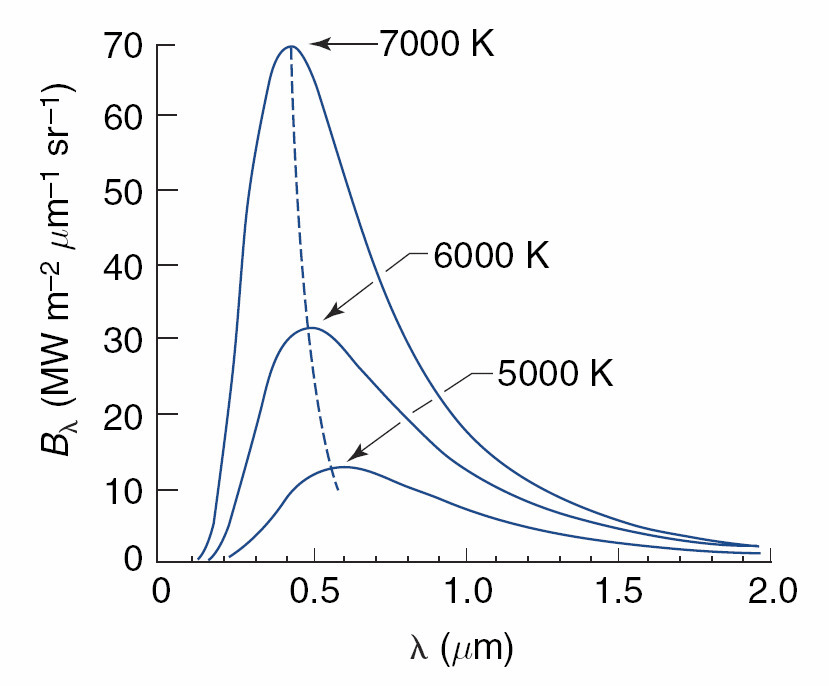
\includegraphics[width=(0.99\linewidth),keepaspectratio]{planckf}
\caption{$B_{\lambda}(T)$ per 3 T.}
\end{figure}

Of two blackbody curves, the one with higher temperature lies entirely above the other:

\begin{align*}
&\PDy{T}{B_{\nu}(T)}=\frac{2h^2\nu^4}{c^2kT^2}\frac{\exp{\frac{h\nu}{kT}}}{[\exp{\frac{h\nu}{kT}}-1]^2}>0\\
&\planckf{\nu}(T\to0)\to0,\ \planckf{\nu}(T\to\infty)\to\infty
\end{align*}

\begin{figure}[!ht]
\centering
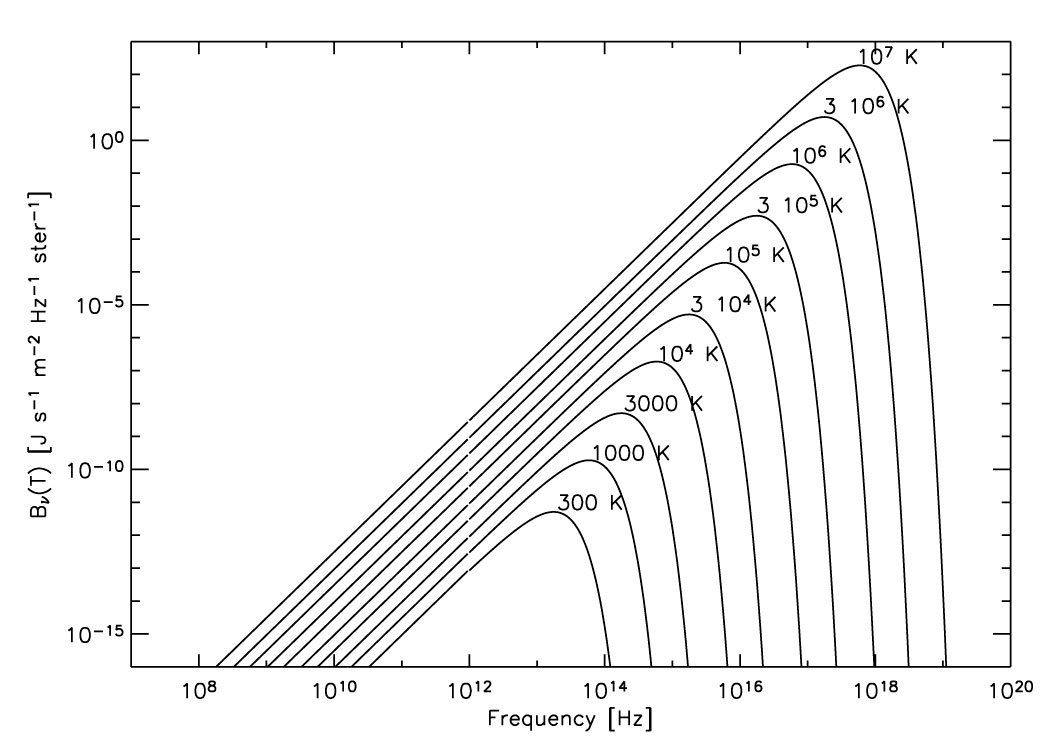
\includegraphics[width=(0.99\linewidth),keepaspectratio]{planckf2}
\caption{Intensit\'a specifica per radiazione di corpo nero in range di T: $\planckf{\nu}(T)$ vs $\nu$.}
\end{figure}

\begin{figure}[!ht]
\centering
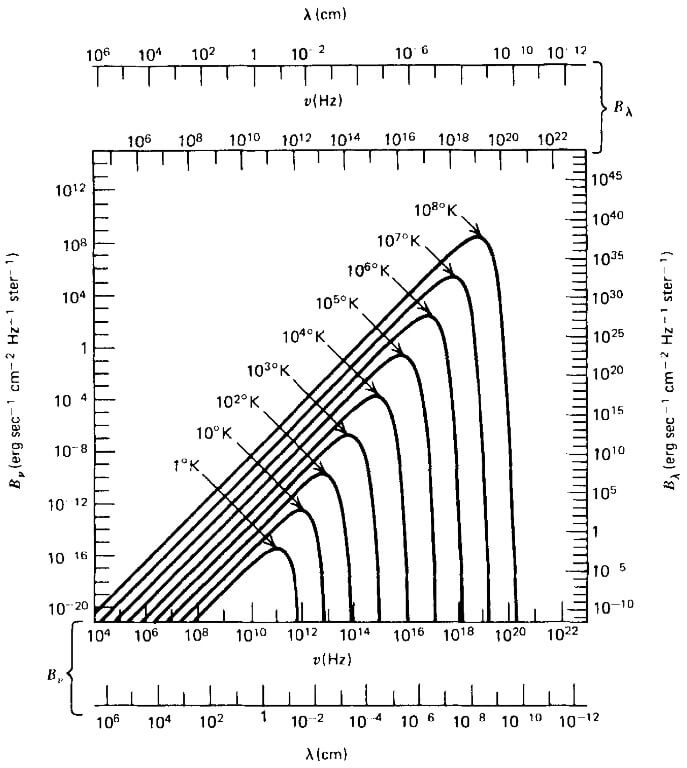
\includegraphics[width=(0.99\linewidth),keepaspectratio]{planckkraus}
\caption{Intensit\'a specifica per radiazione di corpo nero in range di T (cgs). Vedi: Kraus, radio astronomy.}
\end{figure}


\clearpage


\subsection{Energy density of black body radiation.}

\begin{align*}
&u_{\nu}=\frac{4\pi}{c}J_{\nu}\\
&J_{\nu}=\frac{1}{4\pi}\int_{4\pi}\,d\Omega I_{\nu}&\intertext{In thermodynamic equilibrium,}\\
&I_{\nu}=B_{\nu}(T)&\intertext{and is isotropic:}\\
&u_{\nu}=\frac{4\pi}{c}B_{\nu}(T)\\
&u_{\nu}=\frac{8\pi h\nu^3}{c^3}\frac{1}{\exp{\frac{h\nu}{kT}}-1}&\intu{monocromatic energy density of black body radiation.}
\end{align*}

Total energy density:

\begin{align*}
&u=\intzi u_{\nu}\,d\nu=\frac{4\pi}{c}\intzi B_{\nu}(T)\,d\nu\\
&=\frac{4\pi}{c}B(T)\\
&u=\frac{8\pi^5k^4}{15c^3h^3}T^4=aT^4\\
&u=\frac{4\pi}{c}B(T)=\frac{4\pi}{c}\frac{\sigma}{\pi}T^4=aT^4
\end{align*}

\subsection{Radiation pressure.}

In thermodynamic equilibrium (for $\mu_{\nu}=1$), $B_{\nu}=I_{\nu}$ and $I=\intzi I_{\nu}\,d\nu=B(T)$: $B(T)$ is isotropic then $p_r=\frac{1}{3}u$.

\begin{equation*}
p_r=\frac{1}{3}aT^4
\end{equation*}


\section{Degenerate Electron gas.}

\begin{todo}{Degenerate Electron gas}
\end{todo}

\chapter{Legge decadimento radio-attivo}
\PartialToc



\section{Probabilit\'a di decadimento per unit\'a di tempo}
\begin{align*}
&\lambda\\
&=\frac{\text{Probabilit\'a che fra N nuclei 1 decada}}{\text{unit\'a di tempo}}=-\frac{dN}{N}\frac{1}{\text{dt}}
\end{align*}

integro ed ho la legge del decadimento radiativo:
$N(t)=N_0e^{-\lambda t}$.

\section{Attivit\'a}
\begin{align*}
A(t)=\frac{\text{\# decadimenti}}{\text{unit\'a tempo}}=A_0(=\frac{N_0}{\tau})e^{-\lambda t}
\end{align*}

Unit\'a.

Bequerel:
$Bq=\frac{1 \#}{tempo}$.

Curie:
$Ci=3,7 10^{10} \frac{\#}{sec}$.

\section{Vita media}
\begin{align*}
\tau=\frac{\int_0^{\infty}t|\frac{dN}{dt}|dt}{\int_0^{\infty}|\frac{dN}{dt}|dt}
\end{align*}

\section{Tempo di dimezzamento}
$T_{\frac{1}{2}}=\frac{N_0}{2}=N_0e^{-\lambda t_{\frac{1}{2}}}$ cio\'e $t_{\frac{1}{2}}=\tau 0,693$.

\section{Attivit\'a specifica}

Attivit\'a specifica=attivit\'a per unit\'a di massa:

$\lambda\frac{N_A}{A(Numero atomico)}=$.

Attivit\'a emessa durante primo secondo di decadimento di una massa di un grammo.

\section{Branching ratio}

\begin{align*}
&^{40}K\to\\
&\left\{\begin{array}{l} ^{40}Ar \to \lambda_{K,Ar}=0,581 10^{-10} y^{-1} \text{(\Pelectron capture)} \\ ^{40}Ca \to \lambda_{K,Ca}=4,962 10^{-10} y^{-1} \text{(\Pelectron emission)}\\ \end{array} \right.\\
\end{align*}

La probabilit\'a di un decadimento \'e la somma delle ''probabilit\'a parziali'':

\mblock{\lambda_{K,T}=\lambda_{K,Ar}+\lambda_{K,Ca}}

\begin{align*}
&\left\{ \begin{array}{c} ^{40}Ar\\^{40}Ca\\ \end{array} \right\}\\
&= \left\{ \begin{array}{c} ^{40}Ar^0 \\ ^{40}Ca^0 \end{array} \right\}\\
&+ \underbrace{\left\{\begin{array}{c} \frac{\lambda_{K,Ar}}{\lambda_{K,T}}\\ \frac{\lambda_{K,Ca}}{\lambda_{K,T}}\\ \end{array}\right\}}_{\text{Branching ratio}}^{40}K(e^{-\lambda_{k,T}t}-1)
\end{align*}

\section{Total activity of a sample}

The total activity of a sample is the sum of all processes counted per unit of time:

$A=\sum_iA_i=\sum\lambda_in_i$.

\section{Activity of a two elements radioactive chain}

\lbt{N_1(t)=N_0\exp{-\lambda_1 t}}{N_2(t)=N_0\frac{\lambda_1}{\lambda_2-\lambda_1}(\exp{\lambda_1t}-\exp{\lambda_2t})} e \mblock{A_2(t)=\lambda_2N_2(t)=\frac{\lambda_1\lambda_2}{\lambda_2-\lambda_1}(\exp{\lambda_1t}-\exp{\lambda_2t})}

Casi particolari:

\begin{enumerate*}

\item $\lambda_1\ll\lambda_2$ (parent long lived - secular equilibrium).

Approssimo $\exp{-\lambda_1}t\approx1$ quindi \mblock{N_2(t)=N_0\frac{\lambda_1}{\lambda_2}(1-\exp{-\lambda_2 t})}:

as t becomes large nuclei of type 2 are decaying at same rate at which are formed. 


\item $\lambda_1<\lambda_2$ (Transient equilibrium).

Facendo il rapporto fra le attivit\'a
\begin{align*}
\frac{\lambda_2N_2}{\lambda_1N_1}=\frac{\lambda_2}{\lambda_2-\lambda_1}(1-\exp{-(\lambda_2-\lambda_1)t})
\end{align*}

vedo che al crescere di t il rapporto

\begin{align*}
\frac{A_2}{A_1}\abc{\text{t grande}}\frac{\lambda_2}{\lambda_2-\lambda_1}
\end{align*}


\item $\lambda_1>\lambda_2$.

I nuclei parent decadono rapidamente, l'attivit\'a dei nuclei di prima generazione raggiunge un massimo e poi decade con la sua costante caratteristica; $N_2(t)\abc{t\gg\tau_1}N_0\frac{\lambda_1}{\lambda_1-\lambda_2}\exp{-\lambda_2t}$

\end{enumerate*}


\chapter{Onde EM e interazione con materia.}
\PartialToc

\section{Equazioni di Maxwell}

\section{Radiation and equation of radiative equilibrium equilibrium}

\subsection{Radiation.}

\begin{definition}{Specific intensity at P in given direction}
Let $d\sigma$ contain P. At given time there will be rays traversing the surface element in all directions: let us consider specific direction $\hat{s}$. Through every point of $d\sigma$ we can construct cones abutting on $d\sigma$ having axes parallel to $\hat{s}$ direction with solid angles at the apex all equal to definite amount $d\Omega$: this cones define a semi-infinite volume in form of truncated cone.

The radiant energy traversing element of area $d\sigma$ and in volume defined is
\begin{equation*}
I\cos{\theta}\,d\sigma\,d\Omega\,dt
\end{equation*}
where $\theta$ is the angle between the normal to $d\sigma$ and $\hat{s}$ direction.

I is the specific intensity at P in the prescribed direction.
\end{definition}


\begin{definition}{Radiazione omogenea e isotropa.}
$I(P,(\theta,\phi))$ indica l'energia in transito per unit\'a di tempo nel punto P nella direzione definita da $(\theta,\phi)$.

Per radiazione omogenea: \mblock{I(P,(\theta,\phi))=I(P)}.

Per radiazione omogenea e isotropa: \mblock{I(P,(\theta,\phi))=I}.
\end{definition}


\begin{definition}{Flusso radiante attraverso superficie.}
\begin{align*}
&d\Omega=\sin{\theta}\,d\theta\,d\phi&\intd{energy traversing $d\sigma$ in direction defined by $d\Omega$}\\
&I\sin{\theta}\cos{\theta}\,d\theta\,d\phi\,d\sigma\,dt\\
&F=F_+-F_-\\
&=\int_0^{2\pi}\int_0^{\frac{\pi}{2}}I\sin{\theta}\cos{\theta}\,d\theta\,d\phi\\
&+\int_0^{2\pi}\int_{\frac{\pi}{2}}^{\pi}I\sin{\theta}\cos{\theta}\,d\theta\,d\phi
\end{align*}
\end{definition}


\begin{definition}{Densit\'a di energia.}
u \'e la densit\'a di energia radiante cio\'e la quantit\'a di energia per unit\'a di volume in transito per unit\'a di tempo.

u \'e la quantit\'a di energia radiante per unit\'a di volume transiting in the neighborhood of a given point per unit time.

$u_{\nu}\,d\nu$ is the energy density of radiation in interval \mblock{[\nu,\nu+\,d\nu]}.

\begin{align*}
&\frac{1}{c}\iint I\,dV\,d\Omega=\frac{V}{c}\int I\,d\Omega\\
&u=\frac{1}{c}\int\,d\omega I&\intd{per radiazione omogenea:}\\
&u_{\nu}=\frac{4\pi}{c}I_{\nu}\\
&u=\frac{4\pi}{c}I
\end{align*}

\end{definition}

\begin{definition}{emission coefficient}
Consider small element of radiating matter of mass m. The amount of radiating energy emitted in direction specified by $d\Omega$ is
\begin{equation*}
j_{\nu}m\,d\Omega\,dt\,d\nu
\end{equation*}

Necessary condition for $j_{\nu}$ to be isotropic is that mass element is isotropic and is in an isotropic radiation field.

If there are $N_n$ atoms in n state we have
\begin{align*}
&j_{\nu_{nm}}\,d\Omega=\frac{N_n}{\rho}[A_{nm}+B_{nm}I_{\nu_{nm}}h\nu_{nm}\,d\Omega
\end{align*}
\end{definition}


\begin{definition}{Total Absorption coefficient}
A pencil of radiation traversing a medium will be weakened by absorption. Traversing thickness $dr$ the radiation (emergent in phase with incident radiation) changes by
\begin{align*}
&dI_{\nu}=-\kappa_{\nu}\rho I_{\nu}\,dr\\
&I_{\nu}(r)=I_{\nu}(0)\exp{-\int_0^s\kappa_{\nu}\rho\,dr}
\end{align*}
\begin{definition}{Optical depth}
\begin{equation*}
\tau_{\nu}=\int_0^s\kappa_{\nu}\rho\,dr
\end{equation*}
\end{definition}

\end{definition}

\subsection{Radiation pressure}

A quantum of energy $h\nu$ has a momentum $\frac{hy\nu}{c}$ in its direction of propagation. To calculate pressure of radiation at P we have to consider the net rate of transfer of momentum normal to arbitrary surface element $d\sigma$ containing P:
let's consider radiation of frequency $\nu$ incident on surface $d\sigma$ and making angle $\theta$ with the normal, the amount of radiant energy traversing the surface in direction defined by $d\Omega$ is \mblock{I_{\nu}\cos{\theta}\,d\Omega\,d\nu\,d\sigma\,dt} and carries momentum \mblock{\frac{1}{c}I_{\nu}\cos{\theta}\,d\Omega\,d\nu\,d\sigma\,dt} hence normal component of momentum transfer across $d\sigma$ by radiation is
\begin{equation*}
\frac{1}{c}\,d\sigma\,dtI_{\nu}\cos^2{\theta}\,d\Omega\,d\nu
\end{equation*}
hence
\begin{equation*}
p_{rad}(\nu)=\frac{1}{c}\int_0^{2\pi}\int_0^{\pi}I_{\nu}\cos^2{\theta}\sin{\theta}\,d\theta\,d\phi
\end{equation*}

For isotropic radiation field
\begin{align*}
p_{rad}(\nu)=2\pi I_{\nu}\frac{1}{c}\int_0^{\pi}\cos^2{\theta}\sin{\theta}\,d\theta=\frac{4}{3c}\pi I_{\nu}=\frac{1}{3}u_{\nu}
\end{align*}

and, generally,

\begin{equation*}
P_{rad}=\frac{1}{c}\int I\cos^2{\theta}\,d\Omega
\end{equation*}

\subsection{Steady set up in a static medium in LTE.}

For LTE we have $\frac{j_{\nu}}{\kappa_{\nu}}$ depends only on T and $\frac{j_{\nu}}{\kappa_{\nu}}=B_{\nu}(T)$ specific intensity emitted by a black surface.

Equation of transfer
\begin{align*}
&\TDy{s}{I_{\nu_{nm}}}=N_n(A_{nm}+B_{nm}I_{\nu_{nm}})h\nu_{nm}\\
&-N_mB_{mn}h\nu_{nm}I_{\nu_{nm}}\\
&\TDy{s}{I_{\nu_{nm}}}\frac{1}{\rho}=\frac{N_nA_{nm}h\nu_{nm}}{\rho}\\
&-\frac{N_mB_{mn}h\nu_{nm}}{\rho}(1-\frac{N_nB_{nm}}{N_mB_{mn}})I_{\nu_{nm}}
\end{align*}

$j_{\nu}$ include induced emission, is not a scalar in general but include depends on incident intensity $I_{\nu}$.

\begin{align*}
&\TDy{s}{I_{\nu}}\frac{1}{\rho}=\kappa_{\nu}'B_{\nu}-\kappa_{\nu}'I_{\nu}&\intertext{where}\\
&\kappa_{\nu}'=\kappa_{\nu}(1-\exp{-\frac{h\nu}{KT}})\\
&\frac{N_nB_{nm}}{N_mB_{mn}}=\exp{-\frac{h\nu}{KT}}\\
&(\kappa'=\frac{h\nu}{4\pi}(n_1B_{12}-n_2B_{21}))
\end{align*}


\subsection{Radiative equilibrium and equation of transfer for far interior.}

We shall solve
\begin{equation*}
\TDy{s}{I_{\nu}}\frac{1}{\rho}=\kappa_{\nu}'B_{\nu}-\kappa_{\nu}'I_{\nu}
\end{equation*}
under circumstances applicable in star's interior.

Assumption: static, infinite, LTE medium.

A gram of material generate per unit time an amount of mass $\epsilon_{\nu}\,d\nu$ by processes of irreversible character: heat liberated including net gain of heat per unit mass by ''convection'', ''conduction'' and internal energy converted into heat (see subatomic energy source).

Total spontaneous emission per gram per unit time by element mass at temperature T is $4\pi\kappa_{\nu}'B_{\nu}$.

The total absorption less total induced emission is $\opacitynu{}'\int\intensitynu{}\,d\omega$.

Quindi l'eccesso di emissione sull'assorbimento \'e dato da $\opacitynu{}'\int(\blacknu{}-\intensitynu{})\,d\omega$, e in uno stato stazionario deve essere uguale al calore liberato $\epsilon_{\nu}$:

\begin{equation*}
\opacitynu{}'\int(\blacknu{}-\intensitynu{})\,d\omega=\epsilon_{\nu}
\end{equation*}
che \'e l'equazione dell'equilibrio radiativo.

Esprimo la conservazione dell'energia nella forma
\begin{align*}
&\div{\vec{F}_{\nu}}=\epsilon_{\nu}\rho\\
&\div{\text{Stress tensor}}=-\frac{\opacitynu{}'\rho}{c}\vec{F}_{\nu}
\end{align*}

Detto $\tau_{\nu}=\int\opacitynu{}'\rho\,ds$ ho che
\begin{equation*}
\intensitynu{}=\intzi{}\blacknu{}(-\tau_{\nu})\exp{-\tau_{\nu}}\,d\tau_{\nu}
\end{equation*}
L'intensit\'a specifica in un punto e per direzione data \'e la somma dei contributi di emissione di tutti gli elementi di massa sottostanti.

Assumiamo espansione del tipo:
\begin{equation*}
\blacknu{}(-\tau_{\nu})=\blacknu{}(0)-\tau_{\nu}\TDy{\tau_{\nu}}{\blacknu{}}+\frac{1}{2}\tau_{\nu}^2\TtwoDy{\tau_{\nu}}{\blacknu{}}
\end{equation*}
quindi
\begin{align*}
&\intensitynu{}=\blacknu{}(0)-\Dcvar{\tau_{\nu}\TDy{\tau_{\nu}}{\blacknu{}}}{\tau_{\nu}=0}+\Dcvar{\frac{1}{2}\tau_{\nu}^2\TtwoDy{\tau_{\nu}}{\blacknu{}}}{\tau_{\nu}=0}&\intertext{e segue che}\\
&\intensitynu{}=\blacknu{}-\frac{1}{\opacitynu{}'\rho}\nabla_{\hat{s}}\blacknu{}+\frac{1}{\opacitynu{}'\rho}\nabla_{\hat{s}}(\frac{1}{\opacitynu{}'\rho}\nabla_{\hat{s}}\blacknu{})
\end{align*}

The ratio of successive terms are of order of magnitude $\frac{\epsilon}{\overline{\kappa}B}$: in interior of star
\begin{align*}
&\epsilon\approx\SI{100}{\erg\per\gram\per\second}\\
&\kappa\approx\SI{100}{\square\cm\per\gram}\\
&T\approx\SI{e6}{\kelvin}\\
&\frac{100}{100\frac{\sigma}{\pi}\num{e24}}\approx\num{e-19}
\end{align*}

Quandi per i nostri scopi \'e sufficiente scrivere
\begin{equation*}
\intensitynu{}=\blacknu{}-\frac{1}{\opacitynu{}'\rho}\nabla_{\hat{s}}\blacknu{}
\end{equation*}

da cui

\begin{align*}
&u_{\nu}=\frac{1}{c}\int\intensitynu{}\,d\omega=\frac{4\pi}{c}\blacknu{}\\
&u=\frac{4\pi}{c}B=\frac{4\sigma}{c}T^4=aT^4\\
&\vec{F}_{\nu}=-\frac{4\pi}{3\opacitynu{}'\rho}\nabla\blacknu{}&\intertext{(vedi stress tensor $P_{ij}$)}
\end{align*}

In caso di simmetria sferica
\begin{align*}
&F_r(\nu)=-\frac{c}{\opacitynu{}\rho}\TDy{r}{p_r(\nu)}\\
&F_r=-\frac{c}{\kappa\rho}\TDof{r}(\frac{1}{3}aT^4)\\
&\div{\vec{F}}=\frac{1}{r^2}\TDof{r}(r^2F_r)=\epsilon\rho
\end{align*}

\subsection{Radiative transfer in stellar interior (\sch{}).}

\begin{definition}{Opacity.}
Definisco l'opacit\'a come coefficiente d'assorbimanto per grammo: $\kappa\rho\,dl$ \'e la frazione di energia incidente assorbita in $dl$.
\end{definition}

\begin{usefull}{Nearly isotropic radiation.}
All'interno del Sole $\kappa\rho\approx1$ quindi l'approsimazione di radiazione isotropica \'e accettabile.
\end{usefull}

\begin{definition}{Profondit\'a ottica}
\begin{align*}
dI=-In\sigma\,dr=-I\rho\kappa\,dr=-I\,d\tau&\intertext{I=intensit\'a=energia/sec/$cm^2$}
\end{align*}
\end{definition}

Mostro che la deviazione dall'equilibrio termodinamico necessaria per il trasporto di energia in superficie non influisce in maniera rilevante sulla relazione tra densit\'a di energia della radiazione e temperatura della materia tipica dell'equilibrio termico esatto

\begin{equation*}
u=aT^4
\end{equation*}

\begin{figure}[!ht]
\centering
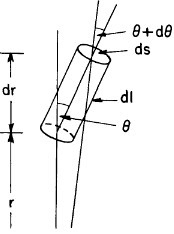
\includegraphics[width=(0.4\textwidth),height=(\textheight-11mm),keepaspectratio]{radiativet}
\caption{Intensity of the radiation field.}
\end{figure}

Geometrical relations
\begin{align*}
&dl=\frac{dr}{\cos{\theta}}\\
&d\theta=-dl\frac{\sin{\theta}}{r}
\end{align*}

Ricavo la relazione esatta tra il flusso di radiazione e il gradiente di temperatura.


Descrivo il campo di radiazione tramite la funzione $I(r,\theta)$ (\si{\erg\per\square\cm\per\second\per\square\radian}) cio\'e l'intensit\'a della radiazione a distanza r dal centro e in direzione inclinata di angolo $\theta$ rispetto a $\vec{r}$.

\begin{align*}
&I(r,\theta)\,d\Omega\,ds-I(r+dr,\theta+d\theta)\,d\Omega\,ds&\intu{gain by radiation entering at bottom surface and loss at top surface}\\
&-I\,d\Omega\,ds*\kappa\rho\,dl&\intu{loss by absorption over the length of the cylinder}\\
&+j\rho\,ds\,dl\frac{d\Omega}{4\pi}&\intu{emission of all matter in the cylinder in direction contained in solid angle $d\Omega$: $j$ rappresenta l'energia emessa da un grammo per secondo in maniera isotropa in tutte le direzioni.}
\end{align*}

\begin{usefull}{Basic equation for radiative transfer.}

\begin{align}\label{eq:radtran}
\PDy{r}{I}\cos{\theta}-\PDy{\theta}{I}\frac{\sin{\theta}}{r}+\kappa\rho I-\frac{1}{4\pi}j\rho=0
\end{align}

\end{usefull}
Fatti:
\begin{itemize}
    \item The equation \ref{eq:radtran} must hold at every points withia a star.
    \item For stellar interior the solution is simplified by the fact that here the radiation field is very nearly isotropic.
\end{itemize}

$I(r,\theta)$ rappresenta la distribuzione di radiazione in tutte le direzioni. Considero i primi momenti di $I$

\begin{align*}
&E(r)=\frac{1}{c}\int I\,d\Omega&\intu{Energy density}\\
&F(r)=\int I\cos{\theta}\,d\Omega&\intu{Radiation flux}\\
&P_R(r)=\frac{1}{c}\int I\cos^2{\theta}\,d\Omega&\intu{Radiation pressure}
\end{align*}

e si ha

\begin{align*}
&\TDy{r}{F}+\frac{2}{r}F+c\kappa\rho u-j\rho=0\\
&\TDy{r}{P_R}+\frac{1}{r}(3P_R-u)+\frac{\kappa\rho}{c}F=0
\end{align*}

\begin{usefull}{quasi-isotropic radiation field: far stellar interio}
Let's represent radiation field at P by
\begin{align*}
&I=I_0+I_1\cos{\theta}+I_2\cos^2{\theta}+\ldots&\intertext{ignoring second term}\\
&\TDy{r}{I_{n-1}}+\kappa\rho I_n=0\\
&|\frac{I_n}{I_{n-1}}|\approx\frac{1}{\kappa\rho R}\approx\num{e-10}
We may restrict to first two terms of the serie
\end{align*}

\end{usefull}

Rappresento il campo di radiazione in un punto tramite la serie

\begin{equation*}
I=I_0+I_1\cos{\theta}+I_2\cos^2{\theta}+\ldots
\end{equation*}

approssimativamente si ha
\begin{equation*}
|\frac{I_n}{I_{n-1}}|\approx\frac{1}{\kappa\rho R}\approx\num{e-10}
\end{equation*}

Inserisco i primi due termini dell'espansione nelle espressioni per i primi momenti di $I$

\begin{align*}
&u=\frac{4\pi}{c}I_0\\
&F=\frac{4\pi}{3}I_1\\
&P_R=\frac{4\pi}{3c}I_0
\end{align*}

quindi
\begin{equation*}
P_R=\frac{1}{3}u
\end{equation*}

L'espressione per l'emissione \'e composta da un contributo per la normale emissione termica e un contributo uguale alla produzione di energia nucleare per grammo per secondo

\begin{equation*}
j=\kappa acT^4+\epsilon
\end{equation*}

Elimino $\epsilon$ tramite la condizione di equilibrio termico
\begin{equation*}
    \TDy{r}{l(r)}=\epsilon\rho4\pi r^2
\end{equation*}

e ottengo

\begin{equation*}
u=aT^4
\end{equation*}


Questa relazione tra la densit\'a di energia della radiazione e la temperatura della materia \'e la stessa che \'e valida per perfetto equilibrio termico: non \'e modificata dalla piccola anisotropia della radiazione nell'interno stellare.

For radiation pressere we have \mblock{P_{rad}=\frac{a}{3}T^4} quindi
\begin{equation*}
H=-\frac{1}{3\kappa\rho}\TDof{r}(acT^4)
\end{equation*}

\clearpage

\section{Local thermodynamic equilibrium.}


\subsection{Thermodynamic equilibrium}

The matter has the same T: radiation field must be homogeneous and isotropic.

The ratio of the emission to the absorption coeffcient for the radiation of frequency $\nu$ in the interior of a homogeneous isotropic medium adiabatically inclosed is equal to the specific intensity of tghe radiation for frequency $\nu$.

\begin{equation*}
j_{\nu}=\kappa_{\nu}I_{\nu}
\end{equation*}

\subsection{Kirchoff's law}

The intensity of radiation emergent from a black surface is indipendent of direction of radiation

\begin{equation*}
\kappa_{\nu}B_{\nu}=j_{\nu}
\end{equation*}

the intensity $I_{\nu}$ of the radiation emitted by a black surface is indipendent of its nature and is a function only of T.

\begin{usefull}{Legge di Kirchoff}
The ratio $\frac{j_{\nu}}{\kappa_{\nu}}$ of the emission to the absorption coefficient of any body in thermodynamical equilibrium depends on temperature only and is indipendent of nature of the body. $\frac{j_{\nu}}{\kappa_{\nu}}$ is equal to specific intensity of the $\nu$ radiation emitted by black surface $I_{\nu}=B_{\nu}$.
\end{usefull}

\subsection{Radiation in adiabatic inclosure at T.}

\begin{align*}
&u=\frac{4\pi}{c}\intzi{}B_{\nu}\,d\nu=aT^4\\
&B(T)=\intzi{}B_{\nu}(T)\,d\nu=\frac{ac}{4\pi}T^4\\
&B(T)=\frac{\sigma}{\pi}T^4&\intertext{$\sigma=\frac{ac}{4}$ is the radiation constant.}
\end{align*}

From QM
\begin{align*}
&B_{\nu}(T)=\frac{2h\nu^3}{c^2}\frac{1}{\exp{\frac{h\nu}{KT}}-1}\\
&B(T)=\frac{2h}{c^2}\intzi{}\frac{\nu^3}{\exp{\frac{h\nu}{KT}}-1}\,d\nu\\
&=\frac{2h}{c^2}(\frac{KT}{h})^4\intzi{}\frac{x^3}{\exp{x}-1}\,dx&\intertext{posto $x=\frac{h\nu}{KT}$}\\
&\intzi{}\frac{x^3}{\exp{x}-1}\,dx\\
&=\intzi{}x^3\exp{-x}(1+\exp{-x}+\exp{-2x}+\ldots)\,dx\\
&6(1+\frac{1}{2^4}+\frac{1}{3^4}+\ldots)\to\frac{\pi^4}{15}
\end{align*}


\section{Emission/absorption coefficient}


\section{Faraday rotation}

\subsection{Faraday rotation in the interstellar medium}

The effect is imposed on light over the course of its propagation from its origin to the Earth, through the interstellar medium. Here, the effect is caused by free electrons and can be characterized as a difference in the refractive index seen by the two circularly polarized propagation modes. Hence, in contrast to the Faraday effect in solids or liquids, interstellar Faraday rotation ($\beta$) has a simple dependence on the wavelength of light ($\lambda$), namely:

\begin{equation*}
\beta= RM \lambda^2
\end{equation*}

where the overall strength of the effect is characterized by RM, the rotation measure. This in turn depends on the axial component of the interstellar magnetic field $B_{\parallel}$, and the number density of electrons $n_e$, both of which vary along the propagation path. In Gaussian cgs units the rotation measure is given by:

 \begin{align*}
&{\displaystyle \mathrm {RM} ={\frac {e^{3}}{2\pi m^{2}c^{4}}}\int _{0}^{d}n_{e}(s)B_{||}(s)\;\mathrm {d} s} {\mathrm {RM}}\\
&={\frac {e^{3}}{2\pi m^{2}c^{4}}}\int _{0}^{d}n_{e}(s)B_{{||}}(s)\;{\mathrm {d}}s
 \end{align*}

or in SI units:

\begin{align*}
 &RM =\frac{e^{3}}{8\pi^{2}\varepsilon_{0}m^2c^3}\int_0^dn_{e}(s)B_{||}(s)\;ds\\
 &\approx (2.62\times 10^{-13}\,T^{-1})\,\int_0^dn_{e}(s)B_{||}(s)\;ds\\
 &RM=\frac{e^{3}}{8\pi^2\varepsilon_{0}m^2c^3}\int_0^dn_{e}(s)B_{\parallel}(s)\;ds\\
 &\approx (2.62\times 10^{-13}\,T^{-1})\,\int_0^dn_{e}(s)B_{\parallel}(s)\;ds
\end{align*}

where $n_e(s)$ is the density of electrons at each point s along the path, $B_{\parallel}(s)$ is the component of the interstellar magnetic field in the direction of propagation at each point s along the path, $e$ is the charge of an electron; $c$ is the speed of light in a vacuum; $m$ is the mass of an electron; $\epsilon_{0}$ is the vacuum permittivity.

The integral is taken over the entire path from the source to the observer.

Faraday rotation is an important tool in astronomy for the measurement of magnetic fields, which can be estimated from rotation measures given a knowledge of the electron number density. In the case of radio pulsars, the dispersion caused by these electrons results in a time delay between pulses received at different wavelengths, which can be measured in terms of the electron column density, or dispersion measure. A measurement of both the dispersion measure and the rotation measure therefore yields the weighted mean of the magnetic field along the line of sight. The same information can be obtained from objects other than pulsars, if the dispersion measure can be estimated based on reasonable guesses about the propagation path length and typical electron densities. In particular, Faraday rotation measurements of polarized radio signals from extragalactic radio sources occulted by the solar corona can be used to estimate both the electron density distribution and the direction and strength of the magnetic field in the coronal plasma.

\subsection{Faraday rotation in the ionosphere}

Radio waves passing through the Earth's ionosphere are likewise subject to the Faraday effect. The ionosphere consists of a plasma containing free electrons which contribute to Faraday rotation according to the above equation, whereas the positive ions are relatively massive and have little influence. In conjunction with the earth's magnetic field, rotation of the polarization of radio waves thus occurs. Since the density of electrons in the ionosphere varies greatly on a daily basis, as well as over the sunspot cycle, the magnitude of the effect varies. However the effect is always proportional to the square of the wavelength, so even at the UHF television frequency of \SI{500}{\mega\hertz} ($\lambda=\SI{60}{\cm}$), there can be more than a complete rotation of the axis of polarization. A consequence is that although most radio transmitting antennas are either vertically or horizontally polarized, the polarization of a medium or short wave signal after reflection by the ionosphere is rather unpredictable. However the Faraday effect due to free electrons diminishes rapidly at higher frequencies (shorter wavelengths) so that at microwave frequencies, used by satellite communications, the transmitted polarization is maintained between the satellite and the ground.

\subsection{Faraday rotation of semiconductors}

GaAs-Faraday rotation spectrum

Due to spin-orbit coupling, undoped $GaAs$ single crystal exhibits much larger Faraday rotation than glass ($SiO_2$). Considering the atomic arrangement is different along the (100) and (110) plane, one might think the Faraday rotation is polarization dependent. However, experimental work revealed an immeasurable anisotropy in the wavelength range from \SIrange{880}{1600}{\nano\meter}. Based on the large Faraday rotation, one might be able to use $GaAs$ to calibrate the B field of the terahertz electromagnetic wave which requires very fast response time. Around the band gap, the Faraday effect shows resonance behavior.

More generally, (ferromagnetic) semiconductors return both electro-gyration and a Faraday response in the high frequency domain. The combination of the two is described by gyroelectromagnetic media, for which gyroelectricity and gyromagnetism (Faraday effect) may occur at the same time.

\section{Fraunhofer lines}

Linee assorbimento.

\begin{figure}[!ht]
\centering
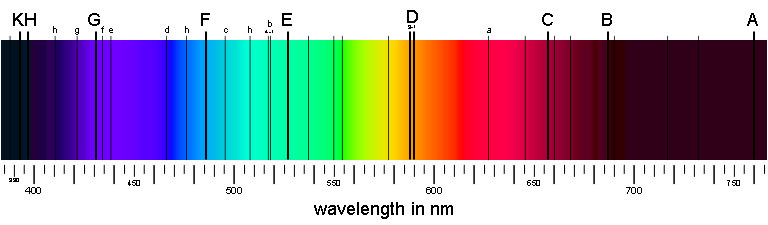
\includegraphics[width=(0.99\textwidth),height=(\textheight),keepaspectratio]{Fraunhofer_lines}
\caption{Linee di Fraunhofer nello spettro solare.}
\end{figure}

\begin{figure}[!ht]
\centering
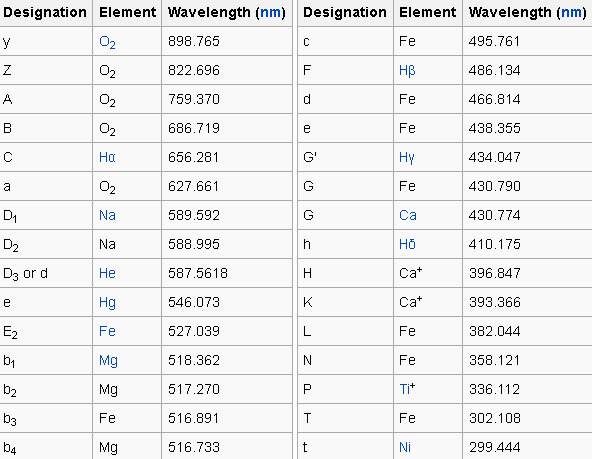
\includegraphics[width=(0.99\textwidth),height=(\textheight),keepaspectratio]{Fraunhoferlambda}
\caption{Lunghezza d'onda delle principali inee di Fraunhofer.}
\end{figure}

\clearpage

\section{Effetto stark}

Classical electrostatics.

The Stark effect originates from the interaction between a charge distribution (atom or molecule) and an external electric field. Before turning to quantum mechanics we describe the interaction classically and consider a continuous charge distribution $\rho(r)$. If this charge distribution is non-polarizable its interaction energy with an external electrostatic potential $V(r)$ is

\begin{align*}
&E_{\mathrm{int}} = \int \rho(\mathbf{r}) V(\mathbf{r}) d\mathbf{r}^3
\end{align*}

If the electric field is of macroscopic origin and the charge distribution is microscopic, it is reasonable to assume that the electric field is uniform over the charge distribution. That is, $V$ is given by a two-term Taylor expansion,

\begin{align*}
&V(\mathbf{r}) = V(\mathbf{0}) - \sum_{i=1}^3 r_i F_i&\intertext{ , with the electric field:}\\
&F_i \equiv -\left. \left(\frac{\partial V}{\partial r_i} \right)\right|_{\mathbf{0}}
\end{align*}

where we took the origin $0$ somewhere within $\rho$. Setting $V(0)$ as the zero energy, the interaction becomes

\begin{align*}
&E_{\mathrm{int}} = - \sum_{i=1}^3 F_i \int \rho(\mathbf{r}) r_i d\mathbf{r} \equiv\\
&- \sum_{i=1}^3 F_i \mu_i = - \mathbf{F}\cdot \boldsymbol{\mu}
\end{align*}

Here we have introduced the dipole moment $\mu$ of $\rho$ as an integral over the charge distribution. In case $\rho$ consists of $N$ point charges $q_j$ this definition becomes a sum

\begin{align*}
&\boldsymbol{\mu} \equiv \sum_{j=1}^N q_j \mathbf{r}_j.
\end{align*}

Perturbation theory.

It is interesting to note that astronomical perturbation applied to a classical hydrogen atom produces a distortion of the electron orbit in a direction perpendicular to the applied electric field.

This effect can be shown without perturbation theory using the relation between the angular momentum and the Laplace-Runge-Lenz vector. Using the Laplace-Runge-Lenz approach, one can see both the transverse distortion and the usual Stark effect. The transverse distortion is not mentioned in most textbooks. This approach can also lead to an exactly solvable approximate model Hamiltonian for an atom in a strong oscillatory field. ''There are few exactly-solvable problems in quantum mechanics, and even fewer with a time-dependent Hamiltonian''

Turning now to quantum mechanics an atom or a molecule can be thought of as a collection of point charges (electrons and nuclei), so that the second definition of the dipole applies. The interaction of atom or molecule with a uniform external field is described by the operator

\begin{align*}
&    V_{\mathrm{int}} = - \mathbf{F}\cdot \boldsymbol{\mu}
\end{align*}.

This operator is used as a perturbation in first- and second-order perturbation theory to account for the first- and second-order Stark effect.
First order

Let the unperturbed atom or molecule be in a g-fold degenerate state with orthonormal zeroth-order state functions \mblock{\psi^0_1, \ldots, \psi^0_g} . (Non-degeneracy is the special case g = 1). According to perturbation theory the first-order energies are the eigenvalues of the g x g matrix with general element

\begin{align*}
&(\mathbf{V}_{\mathrm{int}})_{kl} = \langle \psi^0_k | V_{\mathrm{int}} | \psi^0_l \rangle = -\mathbf{F}\cdot \langle \psi^0_k | \boldsymbol{\mu} | \psi^0_l \rangle, \qquad k,l=1,\ldots, g
\end{align*}
. 

If $g = 1$ (as is often the case for electronic states of molecules) the first-order energy becomes proportional to the expectation (average) value of the dipole operator $\boldsymbol{\mu}$,

\begin{align*}
&E^{(1)} = -\mathbf{F}\cdot \langle \psi^0_1 | \boldsymbol{\mu} | \psi^0_1 \rangle = -\mathbf{F}\cdot \langle \boldsymbol{\mu} \rangle.
\end{align*}

Because a dipole moment is a polar vector, the diagonal elements of the perturbation matrix Vint vanish for systems with an inversion center (such as atoms). Molecules with an inversion center in a non-degenerate electronic state do not have a (permanent) dipole and hence do not show a linear Stark effect.

In order to obtain a non-zero matrix Vint for systems with an inversion center it is necessary that some of the unperturbed functions $\psi^0_i$ have opposite parity (obtain plus and minus under inversion), because only functions of opposite parity give non-vanishing matrix elements. Degenerate zeroth-order states of opposite parity occur for excited hydrogen-like (one-electron) atoms. Such atoms have the principal quantum number n among their quantum numbers. The excited state of hydrogen-like atoms with principal quantum number n is n2-fold degenerate and

\begin{align*}
&n^2 = \sum_{\ell=0}^{n-1} (2 \ell + 1)
\end{align*}, 

where $\ell$ is the azimuthal (angular momentum) quantum number. For instance, the excited n = 4 state contains the following $\ell$ states,

\begin{align*}
&16 = 1 + 3 + 5 +7\ \\
&\Rightarrow\  n=4\hbox{contains}\; s\oplus p\oplus d\oplus f
\end{align*}. 

The one-electron states with even $\ell$ are even under parity, while those with odd $\ell$ are odd under parity. Hence hydrogen-like atoms with n>1 show first-order Stark effect.

The first-order Stark effect occurs in rotational transitions of symmetric top molecules (but not for linear and asymmetric molecules). In first approximation a molecule may be seen as a rigid rotor. A symmetric top rigid rotor has the unperturbed eigenstates

\begin{align*}
&|JKM \rangle = (D^J_{MK})^*\\
&M,K= -J,-J+1,\dots,J 
\end{align*}

with $2(2J+1)$-fold degenerate energy for $|K| > 0$ and $(2J+1)$-fold degenerate energy for $K=0$. Here DJMK is an element of the Wigner D-matrix. The first-order perturbation matrix on basis of the unperturbed rigid rotor function is non-zero and can be diagonalized. This gives shifts and splittings in the rotational spectrum. Quantitative analysis of these Stark shift yields the permanent electric dipole moment of the symmetric top molecule.

\section{Thomson scattering (Coherent Compton effect)}

Thomson scattering cross section valid for \mblock{\frac{h\nu}{m_ec^2}\ll1,\ \lambda\gg\SI{0.02}{\angstrom}}: radiation emitted by oscillating electron with same frequency of impinging EM wave. The energy radiated in unit time by electron whose acceleration is of magnitude a (speed less than c) is \mblock{\TDy{t}{E}=\frac{2}{3}\frac{e^2}{c^3}a^2} with
\begin{equation*}
a=-\frac{eE}{m_e}=-(\frac{eE_0}{m_e})\sin{\omega t}
\end{equation*}

The rate of flow of incoming EM energy across unit area is given by Poynting vector (gaussian unit)
\begin{align*}
&\vec{j}=\frac{c}{4\pi}\vecp{E}{H}\\
&j=\frac{c}{4\pi}E_0^2\sin^2{\omega t}
\end{align*}

The Thomson scattering cross section is
\begin{align*}
&\sigma_0=\frac{\TDy{t}{E}}{j}=\frac{8\pi}{3}a_0^2\\
&=\SI{0.6652e-24}{\square\cm}&\intertext{$a_0=\frac{e^2}{m_ec^2}$ \'e il raggio classico dell'elettrone.}
\end{align*}

\section{Livelli atomici}

\subsection{Energie di ionizzazione}

\begin{align*}
&\SI{13.5984}{\ev}:\chem{^1H}I\to\chem{^1H}II\\
&\SI{24.5873}{\ev}:\chem{^4He}I\to\chem{^4He}II\\
&\SI{54.4177}{\ev}:\chem{^4He}II\to\chem{^4He}III\\
&\SI{7.9024}{\ev}:\chem{_{26}Fe}I\to\chem{_{26}Fe}II\\
&\SI{7.6462}{\ev}:\chem{_{12}Mg}I\to\chem{_{12}Mg}II\\
&\SI{6.1131}{\ev}:\chem{_{20}Ca}I\to\chem{_{20}Ca}II
\end{align*}

\section{Zeeman splitting}

The Zeeman effect can be interpreted in terms of the precession of the orbital angular momentum vector in the magnetic field, similar to the precession of the axis of a spinning top in a gravitational field. 

\subsection{Theoretical presentation}

The total Hamiltonian of an atom in a magnetic field is

\begin{equation*}
H = H_0 + V_M
\end{equation*} 

where $H_0$ is the unperturbed Hamiltonian of the atom, and $V_M$ is the perturbation due to the magnetic field:

\begin{equation*}
V_M = -\vec{\mu} \cdot \vec{B},
\end{equation*}

where $\vec{\mu}$ is the magnetic moment of the atom. The magnetic moment consists of the electronic and nuclear parts; however, the latter is many orders of magnitude smaller and will be neglected here. Therefore,

\begin{equation*}
\vec{\mu} \approx -\frac{\mu_B g \vec{J}}{\hbar},
\end{equation*}

where $\mu_B$ is the Bohr magneton, $\vec{J}$ is the total electronic angular momentum, and g is the Land\'e g-factor. A more accurate approach is to take into account that the operator of the magnetic moment of an electron is a sum of the contributions of the orbital angular momentum $\vec{L}$ and the spin angular momentum $\vec{S}$, with each multiplied by the appropriate gyromagnetic ratio:

\begin{equation*}
\vec{\mu} = -\frac{\mu_B (g_l \vec{L} + g_s \vec{S})}{\hbar}
\end{equation*}

where \mblock{g_l = 1 and g_s \approx 2.0023192} (the latter is called the anomalous gyromagnetic ratio; the deviation of the value from 2 is due to the effects of quantum electrodynamics). In the case of the LS coupling, one can sum over all electrons in the atom:

\begin{equation*}
g \vec{J} = \left\langle\sum_i (g_l \vec{l_i} + g_s \vec{s_i})\right\rangle = \left\langle (g_l\vec{L} + g_s \vec{S})\right\rangle
\end{equation*}

where $\vec{L}$ and $\vec{S}$ are the total orbital momentum and spin of the atom, and averaging is done over a state with a given value of the total angular momentum.

\subsection{Proper zeeman effect}

If the interaction term $V_M$ is small (less than the fine structure), it can be treated as a perturbation; this is the Zeeman effect proper. In the Paschen-Back effect, described below, $V_M$ exceeds the LS coupling significantly (but is still small compared to $H_{0}$). In ultrastrong magnetic fields, the magnetic-field interaction may exceed $H_0$, in which case the atom can no longer exist in its normal meaning, and one talks about Landau levels instead. There are, of course, intermediate cases which are more complex than these limit cases.
Weak field (Zeeman effect)

If the spin-orbit interaction dominates over the effect of the external magnetic field, $\vec{L}$ and $\vec{S}$ are not separately conserved, only the total angular momentum \mblock{\vec{J}= \vec{L} + \vec{S}} is. The spin and orbital angular momentum vectors can be thought of as precessing about the (fixed) total angular momentum vector $\vec{J}$. The (time-)"averaged" spin vector is then the projection of the spin onto the direction of $\vec{J}$:

\begin{equation*}
\vec{S_{avg}} = \frac{(\vec{S} \cdot \vec{J})}{J^2} \vec{J}
\end{equation*}

and for the (time-)"averaged" orbital vector:

\begin{equation*}
    \vec{L_{avg}} = \frac{(\vec{L} \cdot \vec J)}{J^2} \vec{J}
\end{equation*}

Thus,

\begin{equation*}
\langle V_M \rangle = \frac{\mu_B}{\hbar} \vec{J}\left(g_L\frac{\vec{L} \cdot \vec{J}}{J^2} + g_S\frac{\vec{S} \cdot \vec{J}}{J^2}\right) \cdot \vec{B}
\end{equation*}

Using \mblock{\vec{L}= \vec{J} - \vec{S}} and squaring both sides, we get

\begin{equation*}
\vec{S} \cdot \vec{J} = \frac{1}{2}(J^2 + S^2 - L^2) = \frac{\hbar^2}{2}[j(j+1) - l(l+1) + s(s+1)]
\end{equation*}

and: using \mblock{\vec{S}= \vec{J}- \vec{L}} and squaring both sides, we get

\begin{equation*}
 \vec{L} \cdot \vec{J} = \frac{1}{2}(J^2 - S^2 + L^2) = \frac{\hbar^2}{2}[j(j+1) + l(l+1) - s(s+1)]
\end{equation*}

Combining everything and taking \mblock{J_z = \hbar m_j}, we obtain the magnetic potential energy of the atom in the applied external magnetic field,

\begin{align*}
&V_M &= \mu_B B m_j \left[ g_L\frac{j(j+1) + l(l+1) - s(s+1)}{2j(j+1)} + g_S\frac{j(j+1) - l(l+1) + s(s+1)}{2j(j+1)} \right]\\
&= \mu_B B m_j \left[1 + (g_S-1)\frac{j(j+1) - l(l+1) + s(s+1)}{2j(j+1)} \right], \\
&= \mu_B B m_j g_j
\end{align*}

where the quantity in square brackets is the Land\'e g-factor $gJ$ of the atom \mblock{(g_L = 1 and g_S \approx 2)} and $m_j$ is the z-component of the total angular momentum. For a single electron above filled shells $s = 1/2$ and $j = l \pm s$ , the Land\'e g-factor can be simplified into:

\begin{equation*}
g_j = 1 \pm \frac{g_S-1}{2l+1} 
\end{equation*}

Taking $V_m$ to be the perturbation, the Zeeman correction to the energy is

\begin{align*}
&E_Z^{(1)} = \langle nljm_j |H_Z^{'}|nljm_j \rangle\\
&= \langle V_M \rangle_{\Psi} = \mu_B g_J B_{ext} m_j
\end{align*}

Example: Lyman alpha transition in hydrogen

The Lyman alpha transition in hydrogen in the presence of the spin-orbit interaction involves the transitions

\begin{align*}
&2P_{1/2} \to 1S_{1/2}\\
&2P_{3/2} \to 1S_{1/2}
\end{align*}

In the presence of an external magnetic field, the weak-field Zeeman effect splits the $1S1/2$ and $2P1/2$ levels into 2 states each \mblock{(m_j = 1/2, -1/2)} and the $2P3/2$ level into 4 states \mblock{(m_j = 3/2, 1/2, -1/2, -3/2)}. The Land\'e g-factors for the three levels are:

\begin{align*}
&g_J = 2 for 1S_{1/2} (j=1/2, l=0)\\
&g_J = 2/3 for 2P_{1/2} (j=1/2, l=1)\\
&g_J = 4/3 for 2P_{3/2} (j=3/2, l=1)
\end{align*}

Note in particular that the size of the energy splitting is different for the different orbitals, because the $gJ$ values are different. On the left, fine structure splitting is depicted. This splitting occurs even in the absence of a magnetic field, as it is due to spin-orbit coupling. Depicted on the right is the additional Zeeman splitting, which occurs in the presence of magnetic fields.

\subsection{Strong field (Paschen-Back effect)}

The Paschen-Back effect is the splitting of atomic energy levels in the presence of a strong magnetic field. This occurs when an external magnetic field is sufficiently large to disrupt the coupling between orbital ($\vec{L}$) and spin ($\vec{S}$) angular momenta. This effect is the strong-field limit of the Zeeman effect. When $s = 0$, the two effects are equivalent. The effect was named after the German physicists Friedrich Paschen and Ernst E. A. Back.

When the magnetic-field perturbation significantly exceeds the spin-orbit interaction, one can safely assume $[H_{0}, S] = 0$. This allows the expectation values of $L_{z}$ and $S_{z}$ to be easily evaluated for a state $|\psi\rangle$ . The energies are simply

\begin{align*}
&E_{z} = \left\langle \psi \left| H_{0} + \frac{B_{z}\mu_B}{\hbar}(L_{z}+g_{s}S_z) \right|\psi\right\rangle\\
&=E_{0} + B_z\mu_B (m_l + g_{s}m_s)
\end{align*} 

The above may be read as implying that the LS-coupling is completely broken by the external field. However $m_l$ and $m_s$ are still "good" quantum numbers. Together with the selection rules for an electric dipole transition, i.e., \mblock{\Delta s = 0, \Delta m_s = 0, \Delta l = \pm 1, \Delta m_l = 0, \pm 1} this allows to ignore the spin degree of freedom altogether. As a result, only three spectral lines will be visible, corresponding to the \mblock{\Delta m_l = 0, \pm 1} selection rule. The splitting \mblock{\Delta E = B \mu_B \Delta m_l} is independent of the unperturbed energies and electronic configurations of the levels being considered. It should be noted that in general (if $s \neq 0$), these three components are actually groups of several transitions each, due to the residual spin-orbit coupling.

In general, one must now add spin-orbit coupling and relativistic corrections (which are of the same order, known as 'fine structure') as a perturbation to these 'unperturbed' levels. First order perturbation theory with these fine-structure corrections yields the following formula for the Hydrogen atom in the Paschen-Back limit:

\begin{equation*}
E_{z+fs} = E_{z} + \frac{\alpha^2}{2 n^3} \left\{ \frac{3}{4n} - \left[ \frac{l(l+1) - m_l m_s}{l(l+1/2)(l+1) } \right]\right\}. 
\end{equation*}



\section{Scattering/}

Rayleigh scattering applies to the case when the scattering particle is very small (\mblock{x=\frac{2\pi d}{\lambda}\ll1} with a particle size and the whole surface re-radiates with the same phase. Because the particles are randomly positioned, the scattered light arrives at a particular point with a random collection of phases; it is incoherent and the resulting intensity is just the sum of the squares of the amplitudes from each particle and therefore proportional to the inverse fourth power of the wavelength and the sixth power of its size.
 
\subsubsection{From molecules}

The expression above can also be written in terms of individual molecules by expressing the dependence on refractive index in terms of the molecular polarizability $\alpha$, proportional to the dipole moment induced by the electric field of the light. In this case, the Rayleigh scattering intensity for a single particle is given in CGS-units by

\begin{align*}
&I=I_0\frac{8\pi^4\alpha^2}{\lambda^4R^2}(1+\cos^2{\theta})
\end{align*}

\end{document}

\part{Strutture autogravitanti in equilibrio}
%http://jilawww.colorado.edu/~pja/stars02/


\chapter{Equilibrio idrostatico}
\PartialToc

\section{Vincoli osservativi}
Even for the best observed star we observe just 4 basic items

\begin{itemize*}
\item Mass
\item Luminosity
\item Radius
\item  Composition of outer layer
\end{itemize*}

\subsection{Stars: autogravitating bodies in internal equilibrium.}
These items couldn't suffice to derive uniquely the internal structure if it were not for one additional observed item: the constancy of stars over long time intervals (Alghe fossili: luminosit\'a del sole approx. costante per 1 miliardo di anni. Periodo delle Cefeidi lentamente variabile($\tau\approx$ 1 milione yr)): the stellar interior must be in perfect equilibrium.

\section{Fluidodinamica: equazione di Navier-Stokes}

\subsection{Formulazione Euleriana}
Le propriet\'a del fluido come $P,\,T,\,\rho,\,\vec{v},\,\ldots$ sono campi scalari o vettoriali dipendenti dalle variabili posizion $\vec{r}$ e del tempo t: $\vec{r}$ is the position of observer so its time derivative is meaningless without qualification.

Introduco la derivata di Stokes (materiale)\index{Derivata di Stokes (materiale)}

\begin{align*}
D/Dt=\frac{d}{dt}=\frac{\partial}{\partial t}+\scap{v}{\nabla}&\intertext{dove il gradiente  \'e l'operatore tradizionale e la velocit\'a si riferisce a un elemento di fluido}\\
\vec{v}(\vec{r},t)=\frac{d\vec{r}}{dt}=\dot{\vec{r}}&\intertext{$\vec{r}$ \'e una variabile lagrangiana}
\end{align*}



\subsection{Formulazione Lagrangiana.}

Nella formulazione Lagrangiana seguo il moto di ogni dato elemento di fluido: in this description $\vec{r}$ denotes the position of fluid element and is no more an indipendent variable rather is a function of t and (in 3D) of 3 parameter. If the parameters form a position vector which was identical to position vector at $t=0$ then $\vec{r}=\vec{r}(\vec{a},t)$.

The a's don't need to be coordinates in Lagr. desc.: in 1D (spherical symmetry) a may denotes physical properties of the fluid element at some prior time.

In spherically symmetric case it's convenient to take a Lagrangian coordinate instead of r:
we choose m and any other variables dependes on m and t.

For star of constant mass the radius $R=r(M,t)$ vary strongly in time while $0\leq m\leq M$.


\subsection{Leggi di conservazione}

\subsubsection{Conservation of mass}

\begin{align*}
&\PDy{t}{\rho}+\nabla\cdot(\rho\vec{v})=0&\intu{in Eulerian description mass conservation is expressed as continuity equation, and in term of specific volume $v=\frac{1}{\rho}$:}\\
&\frac{1}{v}\TDy{t}{v}=\scap{\nabla}{v}
\end{align*}

\subsubsection{Momentum conservation}

$v_i$ are components of particles velocities:

\begin{align*}
&\exv{v_iv_k}=u_iu_k+\exv{w_iw_k}\\
&P=\frac{1}{3}\rho\exv{|\vec{w}|^2}=\frac{2}{3}U_{kin}\\
&(\\
&u=\frac{1}{\rho}\intzi{}\TDy{p}{n(p)}\epsilon(p)\,dp,\\ &U_{kin}=\intzi{}\TDy{p}{n(p)}\epsilon(p)\,dp\\
&u=\frac{1}{\rho}\intzi{}n\frac{4\pi p^2}{(2\pi mkT)\expy{\frac{3}{2}}}\exp{-\frac{p^2}{2mkT}}(\frac{p^2}{2m})\,dp=\frac{3}{2}\frac{P}{\rho}\\
&\epsilon(p)=mc^2(\sqrt{1+\frac{p^2}{m^2c^2}}-1)\\
&):\\
&u=\frac{1}{\rho}\intzi{}(\frac{c}{kT})^3\frac{n}{2}p^2\exp{-\frac{pc}{kT}}(pc)\,dp=3\frac{P}{\rho}\\
&U_{rad}=aT^4=3P_{rad})\\
&\rho\exv{w_iw_k}=P\delta_{ik}-\pi_{ik}&\intertext{$\pi_{ik}$ is the viscous stress tensor\index{Viscous stress tensor}:}\\
&\pi_{ik}=\rho\exv{\frac{1}{3}|\vec{w}|^2\delta_{ik}-w_iw_k}\\
&\PDof{t}(\rho u_i)+\PDof{x_k}(\rho u_iu_k+P\delta_{ik}-\pi_{ik})=\rho f_i\\
&\rho\TDy{t}{v_i}=-\PDof{x_j}P\indices{_i_j}+\rho f_i&\intu{in eulerian description: $\vec{v}$ is the momentum per unit mass $P$ total pressure tensor (symmetric in order to conserve angular momentum), assume mass conservation.}\\
&\PDy{t}{(\rho v_i)}+\PDof{x_j}(\rho v_iv_j+P_{ij})=\rho f_i&\intu{conservation form, doesn't require mass conservation}\\
&(\rho v_iv_j+P_{ij})&\intu{Rate of flow of momentum of flux\index{Rate of flow of momentum of flux}}
\end{align*}

\subsubsection{Energy conservation}

\begin{align*}
&\PDof{t}[\frac{\rho}{2}(|\vec{u}|^2+\exv{|\vec{w}|^2})]\\
&+\PDof{x_k}[\frac{\rho}{2}\exv{(u_k+w_k)(u_i+w_i)^2}]-\rho f_ku_k=0\\
&\TDof{t}(\frac{1}{2}\vec{v}^2)=-\frac{1}{\rho}\vec{v}\cdot(\nabla\cdot P)+\scap{f}{v}\\
&\PDof{t}(\frac{\rho}{2}|\vec{u}|^2+\rho U)\\
&+\PDof{x_k}[\frac{\rho}{2}|\vec{u}|^2u_k+u_i(P\delta_{ik}-\pi_{ik})\rho Uu_k+F_k]\\
&=\rho u_kf_k&\intu{states that the total fluid energy density is  the sum of a part due to bulk motion $\rho|\vec{u}|^2$ and a part due to random motion $U \rho$; the flux of fluid in k direction consist of translation of bulk of kinetic energy at k component of mean velocity $\frac{\rho}{2}|\vec{u}|^2u_k$, plus enthalpy flux $(\rho U+P)u_k$, plua viscous contribution $-u_i\pi_{ki}$, plus conductive flux $F_k$}
&\rho U=\rho\exv{\frac{1}{2}|\vec{w}|^2}&\intu{$U$ is the specific internal energy}\\
&F_k=\rho\exv{w_k\frac{1}{2}|\vec{w}|^2}&\intu{conduction heat flux}\\
&\PDof{t}\frac{\rho}{2}|\vec{u}|^2+\PDof{x_k}(\frac{\rho}{2}|\vec{u}|^2u_k)\\
&=\rho u_if_i-u_i\PDy{x_i}{P}+u_i\PDy{x_k}{\pi_{ik}}&\intu{work equation}\\
&\PDof{t}(\rho U)+\PDof{x_k}(\rho Uu_k)=-P\PDy{x_k}{u_k}-\PDy{x_k}{F_k}+\Psi&\intu{internal energy equation}\\
&\Psi=\pi_{ik}\PDy{x_k}{u_i}&\intu{rate of viscous dissipation}\\
&\rho\TDy{t}{U}=-P\scap{\nabla}{u}-\scap{\nabla}{F}_{con}+\Psi\intu{internal energy equation in the form of first law of thermodynamic}\\
&-P\scap{\nabla}{u}=-P[\rho\TDy{t}{(\rho\expy{-1})}]&\intu{rate of doing $P\,dV$ work}\\
&-\scap{\nabla}{F}_{con}+\Psi&\intu{rate of adding heat}
\end{align*}

\subsection{First basic equation in Eulerian description}
For gaseus non-rotating single stars without strong magnetic field the only forces acting on a mass element are pressure and gravity.

Scelgo r e t come variabili indipendenti: $\rho(r,t)$, $m(r,t)$.

\begin{align*}
&dm=4\pi r^2\rho\,dr-4\pi r^2\rho v\,dt&\intertext{the first term is the mass contained in a spherical shell of thickness $dr$ and it gives the variation of $m(r,t)$ due to variation of r at constant t:}\\
&\frac{\partial m}{\partial r}=4\pi r^2\rho&\intertext{$\uparrow$ is our first basic eq in E description.}\\
&\frac{\partial m}{\partial t}=-4\pi r^2\rho v&\intertext{explain the last term in first equation that gives the spherically simmetric mass flow out of sphere of constant radius due to velocity v in outward direction in time $dt$}
\end{align*}

Differenziando opportunamente ottengo l'equazione di continuit\'a
\begin{align*}
&\frac{\partial \rho}{\partial t}=-\frac{1}{r^2}\frac{\partial(\rho r^2 v)}{\partial r}&\intertext{$\uparrow$ \'e la forma per simmetria sferica dell'equazione di C:}\\
&\frac{\partial \rho}{\partial t}=-\nabla\cdot(\rho\vec{v})
\end{align*}

\subsection{Connessione tra E. e L. desc.}

For any function of 2 variables if one is substituted $(r,t\to m,t)$ 

\begin{align*}
\frac{\partial}{\partial m}=\frac{\partial}{\partial r}\frac{\partial r}{\partial m}&\intertext{che applicata ad m:}\\
\frac{\partial r}{\partial m}=\frac{1}{4\pi r^2 \rho}&\intertext{$\uparrow$ is the first basic equation in L. desc.}\\
(\frac{\partial}{\partial t})_m=\frac{\partial}{\partial r}(\frac{\partial r}{\partial t})_m+(\frac{\partial}{\partial t})_r&\intertext{$\uparrow$ substantial derivative of hydrodynamic}
\end{align*}


\subsection{Equazione del moto}

Tensore flusso d'impulso

\begin{equation*}
\Pi_{ik}=P\delta_{ik}+\rho v_iv_k
\end{equation*}

Equazione del moto in desc. L
\begin{align*}
&\rho\frac{d\vec{v}}{dt}=-\nabla\cdot P+\rho \vec{f}\\
&\frac{\partial}{\partial t}(\rho v_i)=-\frac{\partial}{\partial x_k}\Pi_{ik}+\rho f_i&\intertext{$\vec{v}$ is the fluid velocity (linear momentum per unit mass), $\vec{f}$ is the total body or external force per unit mass.}
\end{align*}

\subsection{Equazione di Eulero: lowest order solution}

\subsection{Navier-Stokes equation: first order approximation}

\subsection{Fluido incompressibile: equazione di Navier-Stokes}

Per un fluido incompressibile $\scap{\nabla}{v}=0$ e con $\vec{f}=0$ scrivo l'equazione di Navier-Stokes

\begin{align*}
\rho\frac{\partial \vec{v}}{\partial t}=-\rho(\scap{v}{\nabla})\vec{v}-\nabla P+\eta\Laplace\vec{v}\\
\frac{D \vec{v}}{D t}=-\nabla\Phi_g-\frac{1}{\rho}\nabla P+\nu\Laplace\vec{v}&\intertext{viscosit\'a dinamica $\eta=\rho\nu$}\\
\end{align*}

\section{Pressure force and gravitational force}

\subsection{Stima interazione Coulombiana vs gravitazionale}

Energia di legame elettrostatica molto minore di $1\, eV/Barion$ mentre l'energia di autogravitazione per particella \'e $\frac{GMm_P}{R}$: per densit\'a dell'acqua si hanno energie di legame superiore a $1\, eV/Barion$ a partire da masse paragonabili a quelle della terra.

\subsection{Equilibrio meccanico}

All the forces acting on any small volume within the star must compensate each other exactly: we need to consider gravitational force, directed inward, and pressure force directed outward:

Let us consider a small cylindrical volume at distance $r$ from the center, with axis pointin toward the center, with cross section $ds$ and length $dr$. The pressure force acting on this volume will be

\begin{equation*}
-\frac{dP}{dr}\,ds\,dr
\end{equation*}

where P is the pressure, a monotonic decreasing function of r.

The Gravitational force Will be given by (Mass of volume)$\times$(Gravitational acceleration)
\begin{equation*}
\rho\,ds\, dr\, \frac{GM_r}{r^2}
\end{equation*}
where $M_r=\int_0^r\rho4\pi r^2 dr$ is the mass in a sphere of radius $r$.

Setting the two opposing forces equal we obtain the hydrostatic equilibrium condition
\begin{equation*}
\frac{dP}{dr}=-\rho\frac{GM_r}{r^2}
\end{equation*}

\subsection{Constant-density model}

If $\rho=\rho_c=const.$:
\begin{align*}
&m_r=\frac{r^3}{R^3}M\\
&\TDy{m_r}{P}=-\frac{GM}{4\pi R^4}(\frac{m_r}{M})\expy{-\frac{1}{3}}&\intu{Lagrangian form of  \he{}; from integration:}\\
&P=P_c[1-(\frac{m_r}{M})\expy{\frac{2}{3}}]=P_c[1-(\frac{r}{R})^2]\\
&P_c=\frac{3}{8\pi}\frac{GM^2}{R^4}\\
&=\num{1.34e15}(\frac{M}{\msun{}})^2(\frac{R}{\rsun{}})\expy{-4}\si{\dyn\per\square\cm}&\intu{it's a lower limit for centra pressure in hydrostatic object with density decreasing outward.}
\end{align*}
To find temperature distribution we have to specify an equation of state vedi.

\subsection{Molecular weights}

\begin{definition}{$\mu$: Total rest mass per mole of free particles}

Segue dalla definizione di mole che $\mu$, la massa per mole di particelle libere, \'e uguale alla massa media per particella libera in AMU

\end{definition}

\begin{definition}{AMU}
\begin{equation*}
1\si{\atomicmassunit}=\frac{\SI{1}{\gram\per\mole}}{N_A}\approx m_p
\end{equation*}
\end{definition}

For ions it represent a sort of mean mass of an ''average'' ion in the mixture
\begin{align*}
&n_{I,i}=\frac{\si{\mass\per\volume}(I)}{m_I}=\frac{\rho X_IN_A}{\exv{A_i}m_p}\\
&n_I=\sum_in_{I,i}=\rho N_A\sum_i\frac{X_i}{A_i}
\end{align*}

We define the total mean molecular weight of ions such that
\begin{equation*}
n_I=\frac{\rho N_A}{\mu_I},\quad \mu_I=[\sum_i\frac{X_i}{A_i}]\expy{-1}
\end{equation*}


For electrons we must have a prior knowledge of state of ionization for all species. Now I say that $y_i$ is the grade of ionization of specie i so that number density of free electrons associated with nuclear species is
\begin{equation*}
n_{e,i}=y_iZ_in_{I,i}=\rho N_A(\frac{X_i}{A_i})y_iZ_i
\end{equation*}
We call $y_i$ ionization fraction.

\begin{align*}
&n_e=\sum_in_{e,i}=\rho N_A\sum_i(\frac{X_i}{A_i})y_iZ_i=\frac{\rho N_A}{\mu_e}&\intu{total electron number density, that also define the mean molecular weigth per free electron:}\\
&\mu_e=[\sum_i\frac{Z_iX_iy_i}{A_i}]\expy{-1}&\intu{ratio of total number of nucleons to total number of free electrons.}
\end{align*}

The total mean molecular weight is
\begin{align*}
&\mu=[\frac{1}{\mu_I}+\frac{1}{\mu_e}]\expy{-1}\\
&n=n_I+n_e=\frac{\rho N_A}{\mu}
\end{align*}


\subsubsection{Legge gas perfetti}

\begin{align*}
&P=nkT&\intu{con $n=$ particelle/volume}\\
&P=n_{mol}\gasconstant{}T=\frac{\rho}{\mu}\gasconstant{}T=\frac{\rho}{\mu}\gasconstant{}T&\intd{con:}\\
&n_{mol}=\frac{N_{mol}}{V}=\frac{\rho}{\mu}\\
&P=n_{mol}N_A\frac{\gasconstant{}}{N_A}T=nkT
\end{align*}

\section{Tempi caratteristici dell'evoluzione dinamica}

\subsection{Equazione del moto per simmetria sferica}

Considero la condizione di equilibrio idrostatico nella forma
\begin{align*}
&\frac{\partial P}{\partial r}=-g\rho=-\frac{Gm}{r^2}\rho&\intertext{Second basic equation in Eulerian form $\uparrow$ and (multiplying by $\frac{\partial r}{\partial m}=(4\pi r^2\rho)^{-1}$) in Lagrangian form taking m as indipendent variable $\downarrow$}\\
&\frac{\partial P}{\partial m}=-\frac{Gm}{4\pi r^4}
\end{align*}

L'equazione di equilibrio idrostatico \'e un caso particolare di conservazione della quantit\'a di moto: se gli strati della stella effettuano moti radiali accelerati devo considerare l'inerzia dell'elemento:

\begin{align*}
&f_P=-\frac{\partial P}{\partial m}\,dm\\
&f_g=-\frac{g\,dm}{4\pi r^2}=-\frac{Gm}{r^2}\frac{dm}{4\pi r^2}&\intertext{Owing to pressure gradient one spherical shell experience a force per unit area $f_P$ and gravitational force per unit area $f_g$. If if resultant is not zero the mass shell will be accelerated}\\
&\frac{dm}{4\pi r^2}\frac{\partial^2r}{\partial t^2}=f_P+f_g\\
&\frac{1}{4\pi r^2}\frac{\partial^2r}{\partial t^2}=-\frac{\partial P}{\partial m}+-\frac{Gm}{r^2}\frac{1}{4\pi r^2}&\intertext{Pressure gradient alone would produce outward acceleration: $\partial P/\partial m<0$.}
\end{align*}

Se la derivata seconda di r rispetto al tempo si annulla ho l'equazione dell'equilibrio idrostatico. Posso applicare la condizione di equilibrio idrostatico a una classe pi\'u ampia di soluzioni se la forza di gravit\'a e pressione approx si annullano.

Il sistema evolve attraversando stati vicini di quasi-equilibrio.

\subsection{Tempo di free fall}

Supponendo che in qualche regione della stella la risultante delle forza di pressione e di gravit\'a sia diversa da zero per un f: scrivo l'equazione del moto per un elemento di densit\'a $\rho$.
\begin{align*}
&\frac{d^2r}{dt^2}=f\frac{Gm(r)}{r^2}&\intertext{risolvendo per $dt$}\\
&dt\approx(2G\frac{\msun}{\rsun^3})^{-\frac{1}{2}}=10^3\,s=\frac{1}{4}\,hr
\end{align*}

In particolare
\begin{align*}
&\frac{dv}{dt}=\frac{d^2r}{dt^2}=-F\frac{Gm(r)}{r^2}\\
&\begin{array}{c}
F<0: \text{espansione}\\
F=0: \text{equilibrio}\\
0<F<1: \text{collasso}\\
\end{array} \\
&F=1: \text{Free fall } |\frac{\partial^2r}{\partial t^2}|=\frac{R}{t_{ff}}\approx g
\end{align*}

Calcolo il tempo impiegato da una elemento di massa sulla superficie stellare (inizialmente in quiete) a raggiungere il centro

\begin{align*}
&\frac{d^2r}{dt^2}=-\frac{Gm(r)}{r^2}\\
&\frac{1}{2}d(v^2)=-\frac{Gm(r)}{r^2}&\intertext{ho utilizzato}\\
&\frac{d^2r}{dt^2}=\frac{d}{dt}\frac{dr}{dt}=\frac{dr}{dt}\frac{d}{dr}u=u\frac{d}{dr}u\frac{1}{2}\frac{d}{dr}u^2\\
&u^2=2GM(\frac{1}{r}-\frac{1}{R})&\intertext{$\uparrow$ ho integrato tra R e r. Trovo il tempo di caduta $\downarrow$ ($\xi=\frac{r}{R}$: integro da 1 a 0)} \\
&dt=-(\frac{2GM}{R^3})^{-\frac{1}{2}}\frac{d\xi}{\sqrt{\frac{1}{\xi}-1}}\\
&=-(\frac{8\pi G\rho_0}{3})^{-\frac{1}{2}}\frac{\xi}{1-\xi}\,d\xi\\
&t_{ff}=(\frac{3\pi}{32G\rho_0})^{\frac{1}{2}}\\
&t_{ff}(\rho_{IC}\approx10^{-20}gr/cm^3)\approx10^6\,yr\\
&t_{ff}(\rhosun)\approx1\,hr\\
&t_{ff}(\rho_{F}\approx10^8gr/cm^3)\approx1\,s
\end{align*}

\subsection{Tempo di esplosione}

Il tempo caratteristico per l'espansione di una stella ipotetica in cui fosse improvvisamente annullata la fortza di gravit\'a. Definisco il tempo caratteristico tramite $|\frac{\partial^2r}{\partial t^2}|=\frac{R}{t_{exp}^2}$:
\begin{align*}
&|\frac{\partial^2r}{\partial t^2}|\approx\frac{P}{\rho R}&\intertext{Per ricavare $\uparrow$ ho usato l'equazione del moto e}\\
&4\pi r^2\frac{\partial P}{\partial m}=\frac{\partial P}{\partial r}/\rho,\quad \frac{\partial P}{\partial r}\to\frac{P}{R}
\end{align*}

Ottengo $t_{exp}=R\sqrt{\frac{\rho}{P}}$: essendo $\exv{v_s}\approx\sqrt{\frac{P}{\rho}}$ il valore ora trovato corrisponde al tempo impiegato da un'onda sonora prodotta in $r=0$ a raggiungere la superficie 


\subsection{Tempo idrodinamico}
Near hydrodynamic equilibrium $t_{ff}\approx t_{exp}$:

with $g\approx GM/R^2$ ho che il tempo caratteristico impiegato da una stella (dinamicamente stabile) per diluire una piccola perturbazione dell'equilibrio idrostatico \'e:
\mblock{t_{hyd}\approx\sqrt{\frac{R^3}{GM}}\approx\frac{1}{2}(G\overline{\rho})^{-\frac{1}{2}}}.

\subsection{Small amplitude adiabatic sound wave: fundamental pulsation period.}

Consider a perturbation induced by small-amplitude sound wave to travel from center to surface and back.
\begin{align*}
\Pi=\frac{2R}{v_s}&\intertext{is the period for complete traversal}\\
v_s^2=\Dcad{\TDy{\rho}{P}}=\Gamma_1\frac{P}{\rho}
\end{align*}

\section{Stima pressione e temperatura centrale del sole. Gravothermal specific heat.}

\subsection{Pressione centrale}

Per ricavare l'ordine di grandezza della pressione centrale approssimo (con varie sfumature di rozzezza): 
\begin{itemize*}
\item La pressione alle superficie circa 0
\item Gradiente di pressione: $\frac{\partial P}{\partial m}\to\frac{P_0-P_c}{M}$, $$\frac{\partial P}{\partial r}\to\frac{P_0-P_c}{R}$$etc
\end{itemize*}

Utilizzo l'equazione d'equilibrio idrostatico nella forma
\begin{align*}
&\frac{dP}{dm}=-\frac{Gm}{4\pi r^4}&\intertext{$\uparrow$ ottenuta da}\\
&\frac{dP}{dr}=-G\frac{m(r)}{r^2}\rho(r)=-G\frac{m(r)\,dm(r)}{r^24\pi r^2\,dr}
\end{align*}

Assumendo che $\rho_c=\rho(0)\geq\overline{\rho}(r)\geq\overline{\rho}(R)$

\begin{align*}
&P_c\approx\frac{G}{4\pi}\int_0^M\frac{m\,dm}{(\frac{m}{4/3\pi \overline{\rho}})^{\frac{4}{3}}}\\
&\frac{3G}{8\pi}\frac{M^2}{R^4}\leq P_c\leq [\frac{\rho_c}{\overline{\rho}(R)}]^{\frac{4}{3}}\frac{3G}{8\pi}\frac{M^2}{R^4}
\end{align*}


$\pcsun\approx 2\rhosun \frac{G\msun}{\rsun}=6*10^{15}\,dyn/cm^2$ in cgs units ($\SI{1}{\bar}= \SI{e6}{\dyn\per\square\cm} = \num{e6} g*cm^{-1}*s^{-2}$).
 
\subsection{Temperature estimate.}

Using equation of state of an ideal gas (which hold closely in most stars) in the form
\begin{equation*}
P=\frac{k}{m}\rho T
\end{equation*}
where m is the mean molecular weight: for m we use half of proton mass since hydrogen is the most abbundant element and for ionized element $H^+$ and free electron act like two particles of mean mass $\frac{m_p}{2}$.

\begin{align*}
T_c=\frac{P_c}{\rho_c}\frac{\mu}{\gasconstant{}}=P_c\frac{\mu}{\gasconstant{}}\frac{\overline{\rho}}{\rho_c}\frac{4\pi R^3}{3M}&\intertext{sostituendo valore numerici per il sole}\\
T_c\leq3*10^7\,K
\end{align*}

In the media point of the sun, where we suppose the pressure is half  of $\pcsun$ we find:
\begin{equation*}
\tsun\approx10^7\,K
\end{equation*}

These estimate set at once the scene in which we have to work: too hot gasses to contain chemical compounds and hot enough to be highly ionized.

\subsection{Gravothermal specific heat: effetto sulla stabilit\'a delle regioni centrali.}

In termodinamica definisco il calore specifico soggetto a vincoli nella variazioni delle variabili termodinamiche, adesso la condizione \'e che la pressione del gas di una piccola sfera attorno al centro di una stella sia in equilibrio con il peso degli strati che la sovrastano.

Suppongo che a seguito di un'aggiunta di calore nella parte centrale di una stella in equilibrio questa si espanda in maniera omologa $r+\,dr=(1+x)r$


\begin{align*}
&dq=du+Pdv=c_PT_c(\frac{dT_c}{T_c}-\nad{}\frac{dP_c}{P_c})\\
&=c^*T_c\frac{dT_c}{T_c}\\
&c^*=c_P(1-\nad{}\frac{4\delta}{4\alpha-3})&\intertext{$\uparrow$ has the dimension of specific heat per mass unit: gives temperature variation if heat is added to central region $dT_c=\frac{dq}{c*}$.}
\end{align*}

Per un gas ideale monoatomico ($\alpha=\delta=1$, $\nad{}=\frac{2}{5}$) che approssima l'equazione di stato della materia nel centro del sole \'e $c*<0$: ci\'o stabilizza lo stato del sole dato che per $dq>0$ a seguito di fluttuazioni in reaction rate nucleari si ha $dT<0$ e quindi una diminuzione delle stesse.

\section{Stelle in rotazione: forme di equilibrio}

\subsection{Conservazione del momento angolare}

Non sorprende che le stelle ruotino ma che ruotino lentamente. La conservazione del momento angolare applicata al collasso di una nube di particelle fino alla formazione di una stella ci dice che quest'ultima dovrebbe ruotare con $\tau\approx 1\, min$: ci\'o non avviene perch'e si hanno fissione e perdita di materia equatoriale.


\subsection{Equipotential surface}

\begin{figure}[!ht]
\centering
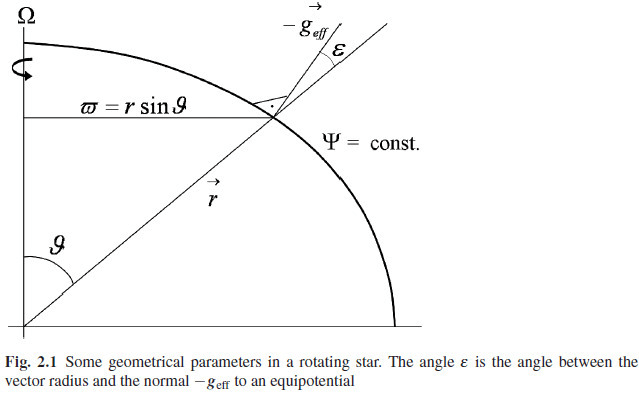
\includegraphics[width=(0.9\textwidth),height=(\textheight-11mm),keepaspectratio]{rotequi}
\caption{Geometrical parameters in rotating star.}
\end{figure}

Considerando la rotazione costante, cio\'e come corpo rigido, l'equazione del moto diventa
\begin{align*}
&\frac{1}{\rho}\nabla P=-\nabla\phi+\frac{1}{2}\Omega^2\nabla(r\sin{\theta})^2\\
&\vec{g}=-\nabla\phi=-\frac{Gm(r)}{r^2}\frac{\vec{r}}{r}
\end{align*}

Introduco un potenziale di rotazione
\begin{equation*}
-\nabla V=\Omega^2(r\sin{\theta})\Rightarrow V=-\frac{1}{2}\Omega^2(r\sin{\theta})^2
\end{equation*}

quindi l'equazione di Poisson diventa

\begin{align*}
&\nabla^2\Psi=4\pi G\rho-2\Omega\\
&\Psi=\phi+V
\end{align*}

e (barotropic stars) l'equazione di equilibrio idrostatico
\begin{equation*}
\frac{1}{\rho}\nabla P=-\nabla\Psi=g_{eff}
\end{equation*}

La forza centrifuga al polo \'e nulla quindi la superficie \'e un equipotenziale di $\frac{GM}{R_p}$, $R(\theta)$ \'e determinato da
\begin{equation*}
\frac{GM}{R(\theta)}+\frac{1}{2}\Omega^2R^2\sin^2{\theta}=\frac{GM}{R_p}
\end{equation*}

\clearpage

\subsection{Fluido in rotazione}

\begin{definition}{Parametro di deformazione}
Rapporto tra l'accelerazione centrifuga e l'accelerazione di gravit\'a: $u$.

\end{definition}

Definisco come parametro per descrivere la deformazione di un fluido autogravitante in rotaziane il rapporto tra l'attrazione gravitazionale e la forza centrifuga all'equatore
\begin{align*}
&u=\frac{\omega^2R^3}{GM}&\intertext{In termini di energia rotazionale e gravitazionale}\\
&E_{Rot}=\frac{1}{5}MR^2\omega^2\\
&E_{Gra}=\frac{3}{5}\frac{GM^2}{R}&\intertext{quindi}\\
&\frac{E_{Rot}}{E_{Gra}}=\frac{1}{3}\frac{\omega^2R^3}{GM}=\frac{1}{3}u\\
&u=\frac{3}{4}\frac{\omega^2}{\pi G \rho}&\intertext{per un corpo omogeneo}
\end{align*}

\subsection{Forma di equilibrio: argomento di Newton.}

Ellissoide di rotazione con semi-assi maggiori $a$ e minore $b=a\sqrt{1-e^2}$, $e$ \'e l'eccentricit\'a.

\begin{figure}[!ht]
\centering
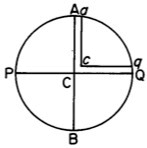
\includegraphics[width=(0.4\textwidth),height=(\textheight-11mm),keepaspectratio]{PEwell}
\caption{Colonne di fluido polare ed equatoriale.}
\end{figure}

Per densit\'a costante:
\begin{align*}
&ag_{eq}(1-u)=bg_{Pol}&\intertext{Primo membro: all'equatore l'accelerazione gravitazionale \'e diluita dall'accelerazione centrifuga (in corpo omogeneo sono proporzionali ad r). Il rapporto fra le due \'e uguale al valore sulla superficie.}\\
&ag_{eq}-a^2\omega^2=g_{Polo}a\sqrt{1-e^2}\\
&\epsilon=\frac{R_{eq}-R_{Polo}}{\exv{R}}=1-\sqrt{1-e^2}\approx\frac{e^2}{2}\\
&=1-\frac{b}{a}&\intertext{$\uparrow$ schiacciamento ai poli}\\
&\frac{g_{Polo}}{g_{eq}}=1+\frac{1}{5}\epsilon+O(\epsilon^2)&\intertext{quindi}\\
&(1-u)=(1-\epsilon)(1+\frac{1}{5}\epsilon)+O(\epsilon^2)\\
&=1-\frac{4}{5}\epsilon+O(\epsilon^2)&\intertext{da cui segue la relazione di Newton:}\\
&\epsilon=\frac{5}{4}u
\end{align*}

\clearpage

\subsection{MacLaurin spheroids}

Chiamo
\begin{align*}
&E_g=\frac{1}{2}\int\rho\Phi\,dV&\intertext{In caso di simmetria sferica: $\frac{d\Phi}{dr}=\frac{Gm(r)}{r^2}$}\\
&\chi=\frac{\omega^2}{2\pi G\rho}
\end{align*}

\begin{align*}
&e^2=\frac{a^2-b^2}{a^2}&\intertext{Along the series of increasing eccentricity $L$ and $E_g$ vary monotonically.}
\end{align*}

If we start with liquid selfgraviting body and feed in angular momentum $L$ also $\omega$ increases and e increses until $e\geq0.9299$ then $\omega$ decreses since moment of inertia increses faster than $\omega$. Before this, at $e=0.8127$, the McLaurin spheroid become unstable: the sequence of configuration shows a bifurcation and we have the Jacobi tri-axial ellipsoid (Jacobi ellipsoid of same mass and angular momentum has lower energi $E=E_g+E_{Rot}$)

\begin{figure}[!ht]
\centering
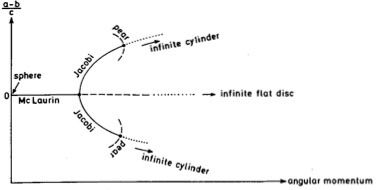
\includegraphics[width=(\textwidth),height=(\textheight-11mm),keepaspectratio]{McL2J}
\caption{Sequence of McLaurin and Jacobian equilibrium configurations of rotating incompressible fluid. a,b,c are 3 axis of an ellipsoid. Solid lines indicate dinamically or secularly stable configurations.}
\end{figure}

If there is a mechanism like friction which can transform macroscopic energy into heat spheroid become ellipsoid: the transition take place on the time-scale of friction.

\begin{figure}[!ht]
\centering
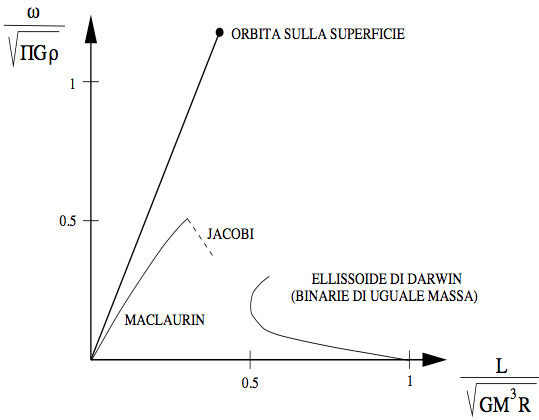
\includegraphics[width=(\textwidth),height=(\textheight-11mm),keepaspectratio]{Eq-shape}
\caption{Relazione $\omega-L$ per figure di equilibrio.}
\end{figure}

\clearpage


\chapter{Teorema del viriale: relazioni statistiche.}
\PartialToc

\section{Teorema del viriale}

\subsection{Thermal/kinetic energy}

\begin{align*}
&K=\int_0^R\overbrace{(+\frac{3}{2}\frac{K}{\mu m_u}T)}^{v^2}\rho 4\pi r^2\,dr\\
&=\overline{+\frac{3}{2}\frac{K}{\mu m_u}T}M\approx\SI{5e48}{\erg}
\end{align*}

\subsection{Teorema del viriale: equilibrio idrostatico.}

\begin{align*}
&\frac{1}{2}\TtwoDy{t}{I}=2K+\Omega\\
&2K=\sum_im_iv_i^2=\sum_i\scap{p_i}{v_i}&\intertext{$\scap{p_i}{v_i}$ measure rate of momentum transfer hence must be related to Pressure}\\
&P=\frac{1}{3}\int_pn(\vec{p})\scap{p}{v}d^3p&\intertext{confrontando le ultime due equazioni si ha:}\\
&2K=3\int_VP\,dV=3\int_M\frac{P}{\rho}\,dm(r)
\end{align*}

Il teorema del viriale si riscrive
\begin{align*}
&\frac{1}{2}\TtwoDy{t}{I}=\int_M\frac{3P}{\rho}\,dm(r)+\Omega&\intertext{Per equilibrio idrostatico}\\
&\frac{1}{2}\TtwoDy{t}{I}=0
\end{align*}

\subsection{$\gamma$-law equation of state.}

Se vale una relazione del tipo \mblock{P=(\gamma-1)\rho u} (per i gas ideali monoatomici con \mblock{\gamma=\frac{5}{3}}, \mblock{P=\frac{2}{3}\rho u})
\begin{equation*}
2K=3(\gamma-1)\int u\,dm
\end{equation*}

$K=E_i$ solo per $\gamma=\frac{5}{3}$: l'energia cinetica \'e uguale all'energia interna totale solo in determinate circostanze.

Il teorema del viriale si riscrive
\begin{equation*}
3(\gamma-1)E_i+\Omega=0
\end{equation*}

e scrivendo l'energia totale $W=E_i+\Omega$ ottengo la relazione esplicita tra energia totale ed energia potenziale gravitazionale per stelle idrostatiche in cui vale la relazione \mblock{P=(\gamma-1)\rho u}
\begin{equation*}
W=\frac{3\gamma-4}{3(\gamma-1)}\Omega
\end{equation*}



\subsection{Gravitational energy.}

Prendo un elemento di massa unitaria a distanza r: la sua energia potenziale dovuta alla massa entro r \'e $-\frac{Gm}{r}$. Quindi l'energia potenziale sommata su tutti gli elementi di massa $dm$ della stella \'e
\begin{equation*}
E_g=-\int_0^M\frac{Gm}{r}\,dm
\end{equation*}

L'energia $-E_g(>0)$ \'e l'energia necessaria ad espandere tutti gli strati a infinito: \'e l'energia liberata quando la stella si forma per contrazione di una gas rarefatto.



\subsection{Internal energy for ideal gas}

Per un gas ideale
\begin{align*}
&\frac{P}{\rho}=\frac{R}{\mu}T=(c_P-c_v)T=(\gamma-1)c_vT=\frac{2}{3}u&\intertext{$\uparrow$ ho usato: $\frac{R}{\mu}=c_P-c_v$. Per un gas monoatomico: $\gamma=\frac{c_P}{c_v}=\frac{5}{3}$ e $u=c_vT$ \'e l'energia interna del gas per unit\'a di massa}
\end{align*}


\subsection{Kinetic energy of the gas.}

\begin{align*}
&dE_k=\frac{3}{2}KT\,dN=\frac{3}{2}RT\,dm\\
&=\frac{3}{2}(c_P-c_V)T\,dm&\intertext{$dN$ \'e il numero di molecole nell'elemento di massa.}\\
&dU=c_VT\,dm&\intertext{quindi ricavo una relazione tra energia cinetica totale delle particelle di gas per unit\'a di massa ed energia interna per unit\'a di massa:}\\
&E_i=\frac{3}{2}(\gamma-1)U
\end{align*}


\subsection{Virial theorem for ideal monoatomic gas in hydrostatic equilibrium}

Il teorema del viriale connette due serbatoi di energia stellare.

\begin{align*}
&\int_0^M\frac{Gm}{r}\,dm=3\int_0^M\frac{P}{\rho}\,dm&\intertext{Il lato sinistro dell'equazione \'e $-E_g$: se la stella si espande/contrae $-E_g$ diminuisce/aumenta (valida per tempi grandi rispetto a $t_{hyd}$). $\uparrow$ deriva dalla seconda equazione fondamentale in forma Lagrangiana moltiplicata per $4\pi r^3$ integrata tra 0 ed M e la relazione $\downarrow$}\\
&\int_0^M4\pi r^3\frac{\partial P}{\partial m}\,dm\\
&=[4\pi r^3P]_0^M-\int_0^M12\pi r^2\frac{\partial r}{\partial m}P\, dm&\intertext{$\uparrow$ ho usato P(M)=0. Seconda equazione F. (equilibrio idrostatico): $\downarrow$}\\
&\frac{\partial P}{\partial m}=-\frac{Gm}{4\pi r^4}\\
&\frac{P}{\rho}=\frac{2}{3}u&\intertext{con $E_i=\int_0^Mu\,dm$:}\\
&E_g=-2E_i
\end{align*}


\subsection{Stima temperatura media.}

Star of uniform temperature and density composed of monoatomic ideal gas. The internal energy density is
\begin{align*}
&U=\frac{3}{2}nkT=\frac{3}{2}\rho\frac{N_AkT}{\mu}\si{\erg\per\cubic\cm}&\intertext{$\mu$ is the mean molecular weight per ion or atom}\\
&P=nkT=\frac{\rho N_AkT}{\mu}\\
&E_i=VU=\frac{3}{2}\frac{MN_AkT}{\mu}&\intertext{il teorema del viriale in questo caso ci dice che $E_i=-\frac{\Omega}{2}$, ($\gamma=\frac{5}{3}$)}\\
&\Omega=-\frac{3}{5}\frac{GM^2}{R}\\
&T=\num{4.09e6}\mu(\frac{M}{\msun{}})\expy{\frac{2}{3}}\rho\expy{\frac{1}{3}}\si{\kelvin}
\end{align*}



\subsection{Teorema del viriale per equazione di stato generale.}

Definisco parametro $\zeta$

\begin{align*}
&\zeta u=3\frac{P}{\rho}&\intertext{Gas ideale:}\\ &\zeta=3(\gamma-1)\xrightarrow{\gamma=\frac{5}{3}}2&\intertext{Pure photon gas:}\\
&P=\frac{1}{3}aT^4, u\rho=aT^4, \zeta=1
\end{align*}

Se $\zeta$ \'e costante nella stella ho una forma pi\'u generale del teorema del viriale
\begin{equation*}
\zeta E_i+E_g=0
\end{equation*}

\subsection{Coupling between $E_i$, $E_g$ and total energy.}

A change in total energy of the configuration is connected with change of its internal energy and with expansion or shrinking:
\begin{equation*}
W=E_i+E_g=(1-\zeta)E_i=\frac{\zeta-1}{\zeta}E_g
\end{equation*}

A gas of finite temperature must radiate
\begin{align*}
&L+\frac{dW}{dt}=0\\
&L=(\zeta-1)\frac{dE_i}{dt}=-\frac{\zeta-1}{\zeta}\frac{dE_g}{dt}
\end{align*}

Ho visto che $\dot{E_g}<0$ per contrazioni di tutti gli strati sferici e per un gas ideale l'equazione precedente da 
\begin{align*}
&L=-\frac{1}{2}\dot{E_g}=\dot{E_i}&\intertext{cio\'e met\'a dell'energia liberata dalla contrazione \'e irradiata nell'universo l'altra met\'a usata per scaldare la stella ($L>0,\dot{E_i}>0$)}
\end{align*}

Stars have negative specific heat: si scaldano mentre perdono energia.

\section{Kelvin-Helmholtz time-scale}

Definisco il tempo caratteristico per l'evoluzione di una stella in collasso: 
\begin{align*}
&L\approx|\frac{dE_g}{dt}|\\
&\tau_{KH}=\frac{E_i}{L}\propto\frac{|E_g|}{L}&\intertext{approssimando rozzamente $E_g$:}\\
&|E_g|\approx\frac{G\overline{m}^2}{\overline{r}}\approx\frac{GM^2}{2R}\\
&t_{KH}\approx\frac{GM^2}{2RL}
\end{align*}
\index{Kelvin-Helmholtz time-scale.}

For the sun $L=3.827 *10^{33}erg/s$ so $t_{KH}\approx1.6*10^7\,yr$.

There are phases in a stellar life when $E_g$ is the main energy source then the star evolves on Kelvin-Helmholtz time-scale.


In any case
\begin{align*}
&\TDy{m}{T}=-\frac{T}{P}\frac{Gm(r)}{4\pi r^4}\nabla\\
&\nabla=\TDly{P}{T}
\end{align*}

\chapter{Energy conservation and energy flux.}
\PartialToc


\section{Third basic equation of stellar structure}

\subsection{Prima legge della termodinamica. Conservazione energia interna.}

If stresses reduce to pure pressure \mblock{P_{ij}=P\delta_{ij}}
\begin{equation*}
\TDy{t}{q}=\TDy{t}{E}+P\TDof{t}(\frac{1}{\rho})=\TDy{t}{E}+P\TDof{t}V
\end{equation*}

equivalent form under asumption 1) $P(\rho,T)$, 2) $E(\rho,T)$, 3) No composition change due to nuclear reaction.

La prima legge della termodinamica esprime la conservazione dell'energia interna (per unit\'a di volume).

Le equazioni equivalenti utilizzando gli esponenti adiabatici $\Gamma_i$

\begin{align*}
&\Gamma_1=\Dcvar{\TDly{\rho}{P}}{Ad},\ \Gamma_3-1=\Dcvar{\TDly{\rho}{T}}{Ad},\\ &\frac{\Gamma_2-1}{\Gamma_2}=\Dcvar{\TDly{P}{T}}{Ad}
\end{align*}

\begin{align*}
&\TDy{t}{\ln{T}}=\frac{\Gamma_2-1}{\Gamma_2}\TDy{t}{\ln{P}}+\frac{\TDy{t}{q}}{c_PT}\\
&\TDy{t}{\ln{P}}=\Gamma_1\TDy{t}{\ln{\rho}}+\frac{\rho(\Gamma_3-1)}{P}\TDy{t}{q}
\end{align*}

Per un gas perfetto $\gamma=\frac{c_P}{c_v}=\Gamma_i$.


\subsection{Flusso di energia locale}
Chiamo $l(r)$ il flusso di energia totale verso l'esterno da una sfera di raggio $r$: energia per sec.

In $l(r)$ sono compresi il trasporto di energia attraverso radiazione, conduzione, convezione: are included only those fluxes that require a temperature gradient.

\begin{figure}[!ht]
\centering
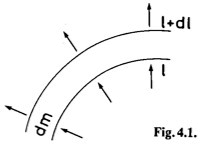
\includegraphics[width=(0.5\textwidth),height=\textheight,keepaspectratio]{localEF}
\caption{Contributo $dl$ da parte dello strato $dm$ fra $r$ e $r+\,dr$.}
\end{figure}

\subsection{Stationary case: only nuclear reaction contributes to $dl$.}

\begin{align*}
&dq=(\epsilon-\PDy{m}{l})\,dt&\intertext{Stato stazionario: il flusso di energia non modifica lo stato termodinamico del gas}\\
&dl=4\pi r^2\rho\epsilon\,dr=\epsilon\,dm\\
&\PDy{m}{l}=\epsilon
\end{align*}

\subsection{Non stationary case: also internal energy and exchange of work contribute to $dl$.}

\begin{align*}
&dq=(\epsilon-\PDy{m}{l})\,dt&\intertext{$\uparrow$ heat added per unit mass to the shell in the interval $dt$. Dalla prima legge della termodinamica ($dq=\,du+P\,dV$) ho:}\\
&\epsilon-\PDy{t}{u}-P\PDy{t}{v}=\epsilon-\PDy{t}{u}+\frac{P}{\rho^2}\PDy{t}{\rho}=\PDy{m}{l}&\intertext{In termini di $T$ e $P$ ho:}\\
&dq=c_P\,dT-\frac{\delta}{\rho}\,dP,\\
&(\delta=-\Dcvar{\PDly{T}{\rho}}{P}=\frac{T}{v}\Dcvar{\PDy{T}{v}}{P})&\intertext{ e quindi:}\\
&\PDy{m}{l}=\epsilon-c_P\PDy{t}{T}+\frac{\delta}{\rho}\PDy{t}{P}&\intertext{$\uparrow$ third basic equation of stellar structure.}
\end{align*}



\subsection{Considero la variazione di stato del gas: contributo alla luminosit\'a negativo/positivo.}

Definisco una funzione che contiene il contributo alla variazione di $l(r)$ per unit\'a di massa dovuta alla variazione dello stato termodinamico del gas

\begin{align*}
&\epsilon_{gas}=-\TDy{t}{q}=-T\PDy{t}{s}=-c_P\PDy{t}{T}+\frac{\delta}{\rho}\PDy{t}{P}\\
&=-c_PT(\frac{1}{T}\PDy{t}{T}-\frac{\nad}{P}\PDy{t}{P})\\
&\delta=-\Dcvar{\PDly{T}{\rho}}{P}=\frac{T}{v}\Dcvar{\PDy{T}{v}}{P}\\
&\nad{}=\Dcvar{\PDly{P}{T}}{s}=\frac{P\delta}{T\rho c_P}
\end{align*}

Surface luminosity of an expanding star can be smaller than energy produced in central core by nuclear reaction ($\epsilon>0$) since part of it is used to expand the star ($\epsilon_g<0$).

\subsection{Complete local energy equation}
La terza equazione fondamentale della struttura stellare \'e
\begin{align*}
&\PDy{m}{l}=\epsilon-c_P\PDy{t}{T}+\frac{\delta}{\rho}\PDy{t}{P}\\
&=\epsilon-\epsilon_{\nu}+\epsilon_g\\
&L_{\nu}=\int_0^M\epsilon_{\nu}\,dm&\intertext{$\uparrow$ neutrino luminosity. Condizioni al contorno:}\\
&l(0)=0\\
&l(R)=L
\end{align*}

\subsection{Energy conservation: total energy.}

Energia totale di una stella
\begin{align*}
&W=E_{Macro}+E_g+E_i+E_n&\intertext{$E_{Macro}$ is the kinetic energy of radial motion, $E_n$ is the nuclear energy content of the whole star. Energy balance:}\\
&\TDof{t}(E_{Macro}+E_g+E_i+E_n)+L+L_{\nu}=0&\intertext{Ottengo la stessa equazion $\uparrow$ integrando l'equazione locale rispetto a $dm$:}\\
&\int_0^M\,dm(\PDy{m}{l})=\int_0^M\,dm(\epsilon-\epsilon_{\nu}+\epsilon_{gas})\\
&\int\PDy{m}{l}=L,\quad\int-\epsilon_{\nu}\,dm=-L_{\nu},\\
&\int\epsilon\,dm=-\dot{E_n}&\intertext{Considero l'integrale di $\epsilon_{gas}$:}\\
&\int\,dm[-\PDy{t}{u}+\frac{P}{\rho^2}\PDy{t}{\rho}]=-\TDy{t}{E_i}-\TDy{t}{E_g}&\intertext{Il primo termine nelle parentesi quadre da}\\
&\int\,dm(-\PDy{t}{u})=-\TDy{t}{E_i}&\intertext{Per riconoscere il secondo derivo rispetto al tempo $E_g$ e uso il teorema del viriale \mblock{E_g=-2E_i=-\int\,dm3\frac{P}{\rho}}:}\\
&\dot{E_g}=-3\int_0^M\frac{\dot{P}}{\rho}\,dm+3\int_0^M\frac{P}{\rho^2}\dot{\rho}\,dm&\intertext{(Ricordo che:)}\\
&(-E_g=\int_0^M\frac{Gm}{r}\,dm=3\int_0^M\frac{P}{\rho}\,dm)&\intertext{Dalla condizione di equilibrio idrostatico ($E_{Macro}=0$) ricavo:}\\
&-3\int_0^M\frac{\dot{P}}{\rho}\,dm=\int_0^M4\pi r^3\PDy{m}{\dot{P}}\,dm\\
&=4\int_0^M\frac{Gm}{r}\frac{\dot{r}}{r}\,dm=4\dot{E_g}
\end{align*}

Per recuperare il termine $E_{Macro}$ devo usare l'equazione del moto
\begin{equation*}
\frac{1}{4\pi r^2}\PtwoDy{t}{r}=-\PDy{m}{P}-\frac{Gm}{4\pi r^4}
\end{equation*}
invece dell'equazione dell'equilibrio idrostatico.




\section{Time-scale consideration: sequenza principale, stelle pulsanti}

\subsection{Nuclear time-scale}

I consider a star balancing its energy loss by release of nuclear energy.

\begin{align*}
&\tau_n=\frac{E_n}{L}&\intertext{$E_n$ is the energy reservoir from which nuclear energy can be released. Hydrogen burning release:}\\
&Q=6.8*\sci{18}\,erg\,g^{-1}&\intertext{for a sun of only hydrogen}\\
&E_n=Q\msun=1.25*\sci{52}\,erg,\\
&\lsun=4*\sci{33}\,erg/\,sec\\
&\tau_n=3*\sci{18}s=\sci{11}\,yr
\end{align*}

\subsection{Ordine di grandezza termini energy equation}

Condizione $\tau_n\gg\tau_{KH}\gg\tau_{Hyd}$.

\begin{align*}
&|\PDy{m}{l}|\approx\frac{L}{M}\approx\frac{E_i}{\tau_{KH}M}\\
&\epsilon\approx\frac{L}{M}\approx\frac{E_n}{M\tau_n}\approx\frac{E_i}{\tau_{KH}M}&\intertext{$\uparrow$: $L$ \'e la stessa sia che la fonte di energia sia nucleare sia che sia l'energia potenziale gravitazionale. Introduco un tempo che caratterizza una determinata fase evolutiva della stella:}\\
&|c_P\PDy{t}{T}|\approx\frac{c_PT}{\tau}\approx\frac{E_i}{\tau M}\\
&|\frac{\delta}{\rho}\PDy{t}{P}|\approx\frac{c_PT}{\tau}\approx\frac{E_i}{\tau M}&\intertext{$\uparrow$ ho usato:}\\
&P=\frac{\rho}{\mu}RT,\ \delta=\frac{T}{v}\Dcvar{\PDy{T}{v}}{P},\\
&c_P=\Dcvar{\PDy{T}{q}}{P}=\Dcvar{\PDy{T}{u}}{P}+P\Dcvar{\PDy{T}{v}}{P}
\end{align*}

\subsection{Stelle di sequenza}

Nel caso $\tau\gg\tkh$ posso trascurare le derivate rispetto al tempo $(|\epsilon_g|\ll\epsilon)$, the energy equation becomes
\begin{align*}
\PDy{m}{l}=\epsilon&\intertext{This happens,ie, if H and He consumption sturns the evolution: $\tau=\tau_n$ and we have mechanical and thermal equilibrium}
\end{align*}

\subsection{Stelle pulsanti}

Nel caso $\tau\ll\tkh$ 
\begin{align*}
&|c_P\PDy{t}{T}|\approx|\frac{\delta}{\rho}\PDy{t}{P}|&\intertext{e cancellarsi a vicenda visto che $\TDy{t}{q}\approx0$ (change nearly adiabatic): a relatively small deviation from strictly adiabatic change can still be of order $\epsilon$. $\epsilon_g$ cannot be neglected.}
\end{align*}

For a pulsationg stars with \mblock{\tau=\thydro\ll\tkh} the variable luminosity is not due to changes of $\epsilon$ but $\epsilon_g$.


\part{Trasporto radiativo. Stabilit\'a rispetto a perturbazioni dello stato interno. Trasporto convettivo.}


\chapter{Transport of energy by radiation and conduction.}
\PartialToc

\section{Radiative transfer}

Photons emitted thermally in hotter regions and absorbed in cooler transfer energy. The effectiveness depends on thermal gradient and ability of the photons to travel freely (among others).The rate of radiative energy transport will be proportional to gradient of fourth power of T.

The reduction of intensity of a beam of photons passing through matter is
\begin{align*}
&\TDy{x}{I}=-\overline{\kappa}\rho I\\
&dI_{\nu}=-\kappa_{\nu}\rho I_{\nu}\,ds
\end{align*}



\subsection{Absorption/scattering coefficients}

$\kappa_{\nu}$ is the mass absorption coefficient: it includes processes of absorption and scattering. In star's interior where matter is completely ionized the bulk of scattering occurs from Thomson scattering by free electrons whereas in cool atmosphere may be due to molecular scattering.

\begin{align*}
&dI_{\nu}=-\kappa_{\nu a}\rho I_{\nu}\,ds\\
&dI_{\nu}=-\kappa_{\nu s}\rho I_{\nu}\,ds\int_{\Omega'}p(\cos{\theta'})\frac{d\Omega'}{4\pi}
\end{align*}
$p(\cos{\theta'})$ is the scattering phase function which gives angular distribution of scattered energy removed from the beam: for Rayleigh scattering $p(\cos{\theta'})=1+\cos^2{\theta'}$.

\subsection{Emission of photons: kirchhoff law}

$j_{\nu}(\theta)$ represents the true emission of radiation of freq. $\nu$ per unit frequency interval in direction $\theta$ per unit solid angle from each gram of stellar matter. The specific intensity of radiation at angle $\theta$ will be increased by

\begin{align*}
&dI_{\nu}(\theta)=j_{\nu }\rho\,ds&\intertext{assumption that stellar interior is in local thermodynamic equilibrium: matter radiates spontaneously in stellar interior as it would in thermodynamic equilibrium: stellar matter is assumed to have temperature T and assumption of local thermodynamic equilibrium is that matter at T radiates exactly as it would if it were in surroundings in thermodynamic equilibrium at same T  :}\\
&I(\theta)=\frac{c}{4\pi}u\ (+\frac{3}{3\pi}H\cos{\theta})&\intertext{sine T gradient is small compared to mean free path of photns in stellar interior the photons are absorbed at same temperature they are emitted. Condition for LTE:}\\
&j_{\nu}=\kappa_{\nu a}\frac{cu_{\nu}}{4\pi}=\kappa_{\nu a}B_{\nu}(T)&\intertext{kirchhoff law}
\end{align*}

Part of the emissions contained in kirchhoff law is spontaneous emission resulting only from T and part is induced emission. The induced emission comes from atomic transitions caused by radiation field and produes radiation with same freq. and moving in same pencil of direction as incident radiation.

\begin{usefull}{Fraction of total emission that is spontaneous}

\begin{align*}
&\frac{\text{Spontaneous}}{\text{Total}}=\frac{N_iA_{ij}}{N_iA_{ij}+N_iB_{ij}u_{\nu_{ij}}}\\
&=\frac{1}{1+(B_{ij}/A_{ij})u_{\nu_{ij}}}
&\intertext{where $\frac{1}{4\pi}N_iA_{ij}$ is a spontaneous transition rate per unit solid angle, $\frac{1}{4\pi}N_iB_{ij}u_{\nu_{ij}}$ is the rate of photons emission (in same direction of incident photons) per unit solid angle, induced by encounters of atoms in state i with photons $\nu_{ij}$}\\
&\frac{\text{Spontaneous}}{\text{Total}}=1-\exp{-\frac{h\nu}{kT}}&\intu{Qm radiation theory requires that this ratio of spontaneous to total emission in local thermodynamic equilibrium apply to any mechanism of true absorption}
\end{align*}

there are mechanism other than transitions between atomic states that represent true emission/absorption: ionization is a true absorption, whereas inverse process is true emission.

\begin{definition}{Induced ionization/recombination}
QM can be show that radiative recombination of ion and electrons with emission of a photon $\nu_{ij}$ can be induced by presence of second photon $\nu_{ij}$.
\end{definition}

One reaches a ratio of spontaneous emission for radiative recombination to total emission by radiative recombination equal to that for atomic transitions.



\end{usefull}

\subsection{Slightly anisotropic radiation field in stellar interior}

One must be cautious to avoid making a mistake in extending properties of radiation computed for condition of local thermodynamic equilibrium to slightly anisotropic radiation field in stellar interior.

If deviation from strict thermodynamic equilibrium occur emission must be separated into two terms: spontaneous emission is still determined by T of matter and the source function is $B_{\nu}(T)$ whereas the induced emission is proportional to actual specific intensity of radiation $I_{\nu}(\theta)$ instead of $B_{\nu}(T)$:
\begin{equation*}
j_{\nu}(\theta)=\kappa_{\nu a}(1-\exp{-\frac{h\nu}{kT}})B_{\nu}(T)+\kappa_{\nu a}\exp{-\frac{h\nu}{kT}}I_{\nu}(\theta)
\end{equation*}

\subsection{Energy introduced into pencil by scattered photons}

Energy scattered per unit solid angle into pencil moving in direction $(\theta,\phi)$ from a pencil in direction $(\theta',\phi')$:
\begin{equation*}
j_{\nu,scat}=\kappa_{\nu s}\frac{1}{4\pi}\int_0^{\pi}\int_0^{2\pi}p(\theta,\phi,\theta',\phi')I_{\nu}(\theta',\phi')\sin{\theta'}\,d\theta'\,d\phi'
\end{equation*}

\subsection{Energy balance: equation of transfer}

We consider a cylinder with axis along $(\theta,\phi)$
\begin{align*}
&\Dcvar{\TDy{t}{Q}}{top}=-I_{\nu}(r+dr,\theta)\,d\Omega&\intu{power exiting from top}\\
&\Dcvar{\TDy{t}{Q}}{bot}=I_{\nu}(r,\theta)\,d\Omega&\intu{power entering from bottom}\\
&\Dcvar{\TDy{t}{Q}}{abs}=-(\kappa_{\nu a}+\kappa_{\nu s})\rho I_{\nu}(r,\theta)\,dl\,d\Omega&\intu{power per unit area absorbed during transit of cylinder}\\
&\Dcvar{\TDy{t}{Q}}{emis}=\kappa_{\nu a}\rho\,dl[(1-\exp{-\frac{h\nu}{kT}})B_{\nu}(T)\\
&+\exp{-\frac{h\nu}{kT}}I_{\nu}(\theta)]\,d\Omega+\kappa_{\nu s}\rho\,dl\frac{d\Omega}{4\pi}*\\
&\iint p(\theta,\phi,\theta',\phi')I_{\nu}(r,\theta',\phi')\sin{\theta'}\,d\theta'\,d\phi'
\end{align*}

From energy conservation \mblock{\Dcvar{\TDy{t}{Q}}{tot}=0}:

\begin{align*}
&I_{\nu}(r+dr,\theta)-I_{\nu}(r,\theta)=\PDy{r}{I_{\nu}}\,dr=\\
&-(\kappa_{\nu a}+\kappa_{\nu s})\rho I_{\nu}(r,\theta)\,dl\\
&+(1-\exp{-\frac{h\nu}{kT}})B_{\nu}(T)\kappa_{\nu a}\rho\,dl\\
&+\exp{-\frac{h\nu}{kT}}I_{\nu}(\theta)\kappa_{\nu a}\rho\,dl\\
&+\kappa_{\nu s}\frac{\rho\,dl}{4\pi}*\int p(\theta,\phi,\theta',\phi')I_{\nu}(r,\theta',\phi')\,d\Omega'
\end{align*}

Using \mblock{dr/dl=\cos{\theta}} and \mblock{\kappa_{\nu a}^*=\kappa_{\nu a}(1-\exp{-\frac{h\nu}{kT}})}:

\begin{align*}
&\frac{1}{\rho\,dl}\PDy{r}{I_{\nu}}\,dr=\frac{1}{\rho}\PDy{r}{I_{\nu}}\cos{\theta}\\
&=-(\kappa_{\nu a}^*+\kappa_{\nu s})I_{\nu}(r,\theta)+\kappa_{\nu a}^*B_{\nu}(T)\\
&+\kappa_{\nu s}\frac{1}{4\pi}*\int p(\theta,\phi,\theta',\phi')I_{\nu}(r,\theta',\phi')\,d\Omega'
\end{align*}

It's the desired equation of radiative transfer for plane parallel atmosphereunder LTE.

\subsection{Photon gas}

Assuming polar axis parallel to direction of net flow.

\begin{align*}
&P_r=\frac{1}{3}\intzi{}\frac{h\nu}{c}cn(\nu)\,d\nu\\
&I(\theta)\,d\Omega=cu(\theta)\,d\Omega&\intu{$u(\theta)\,d\Omega$ represent energy density of radiation moving at angle $\theta$ in $d\Omega$}\\
&H=\int\,d\Omega I(\theta)\cos{\theta}&\intertext{stellar radiation is anisotropic in radial direction}\\
&I(\theta)\approx\frac{c}{4\pi}u+\frac{3}{4\pi}H\cos{\theta}+\ldots&\intu{the second term is much smaller than the first}
\end{align*}

\begin{figure}[!ht]
\centering
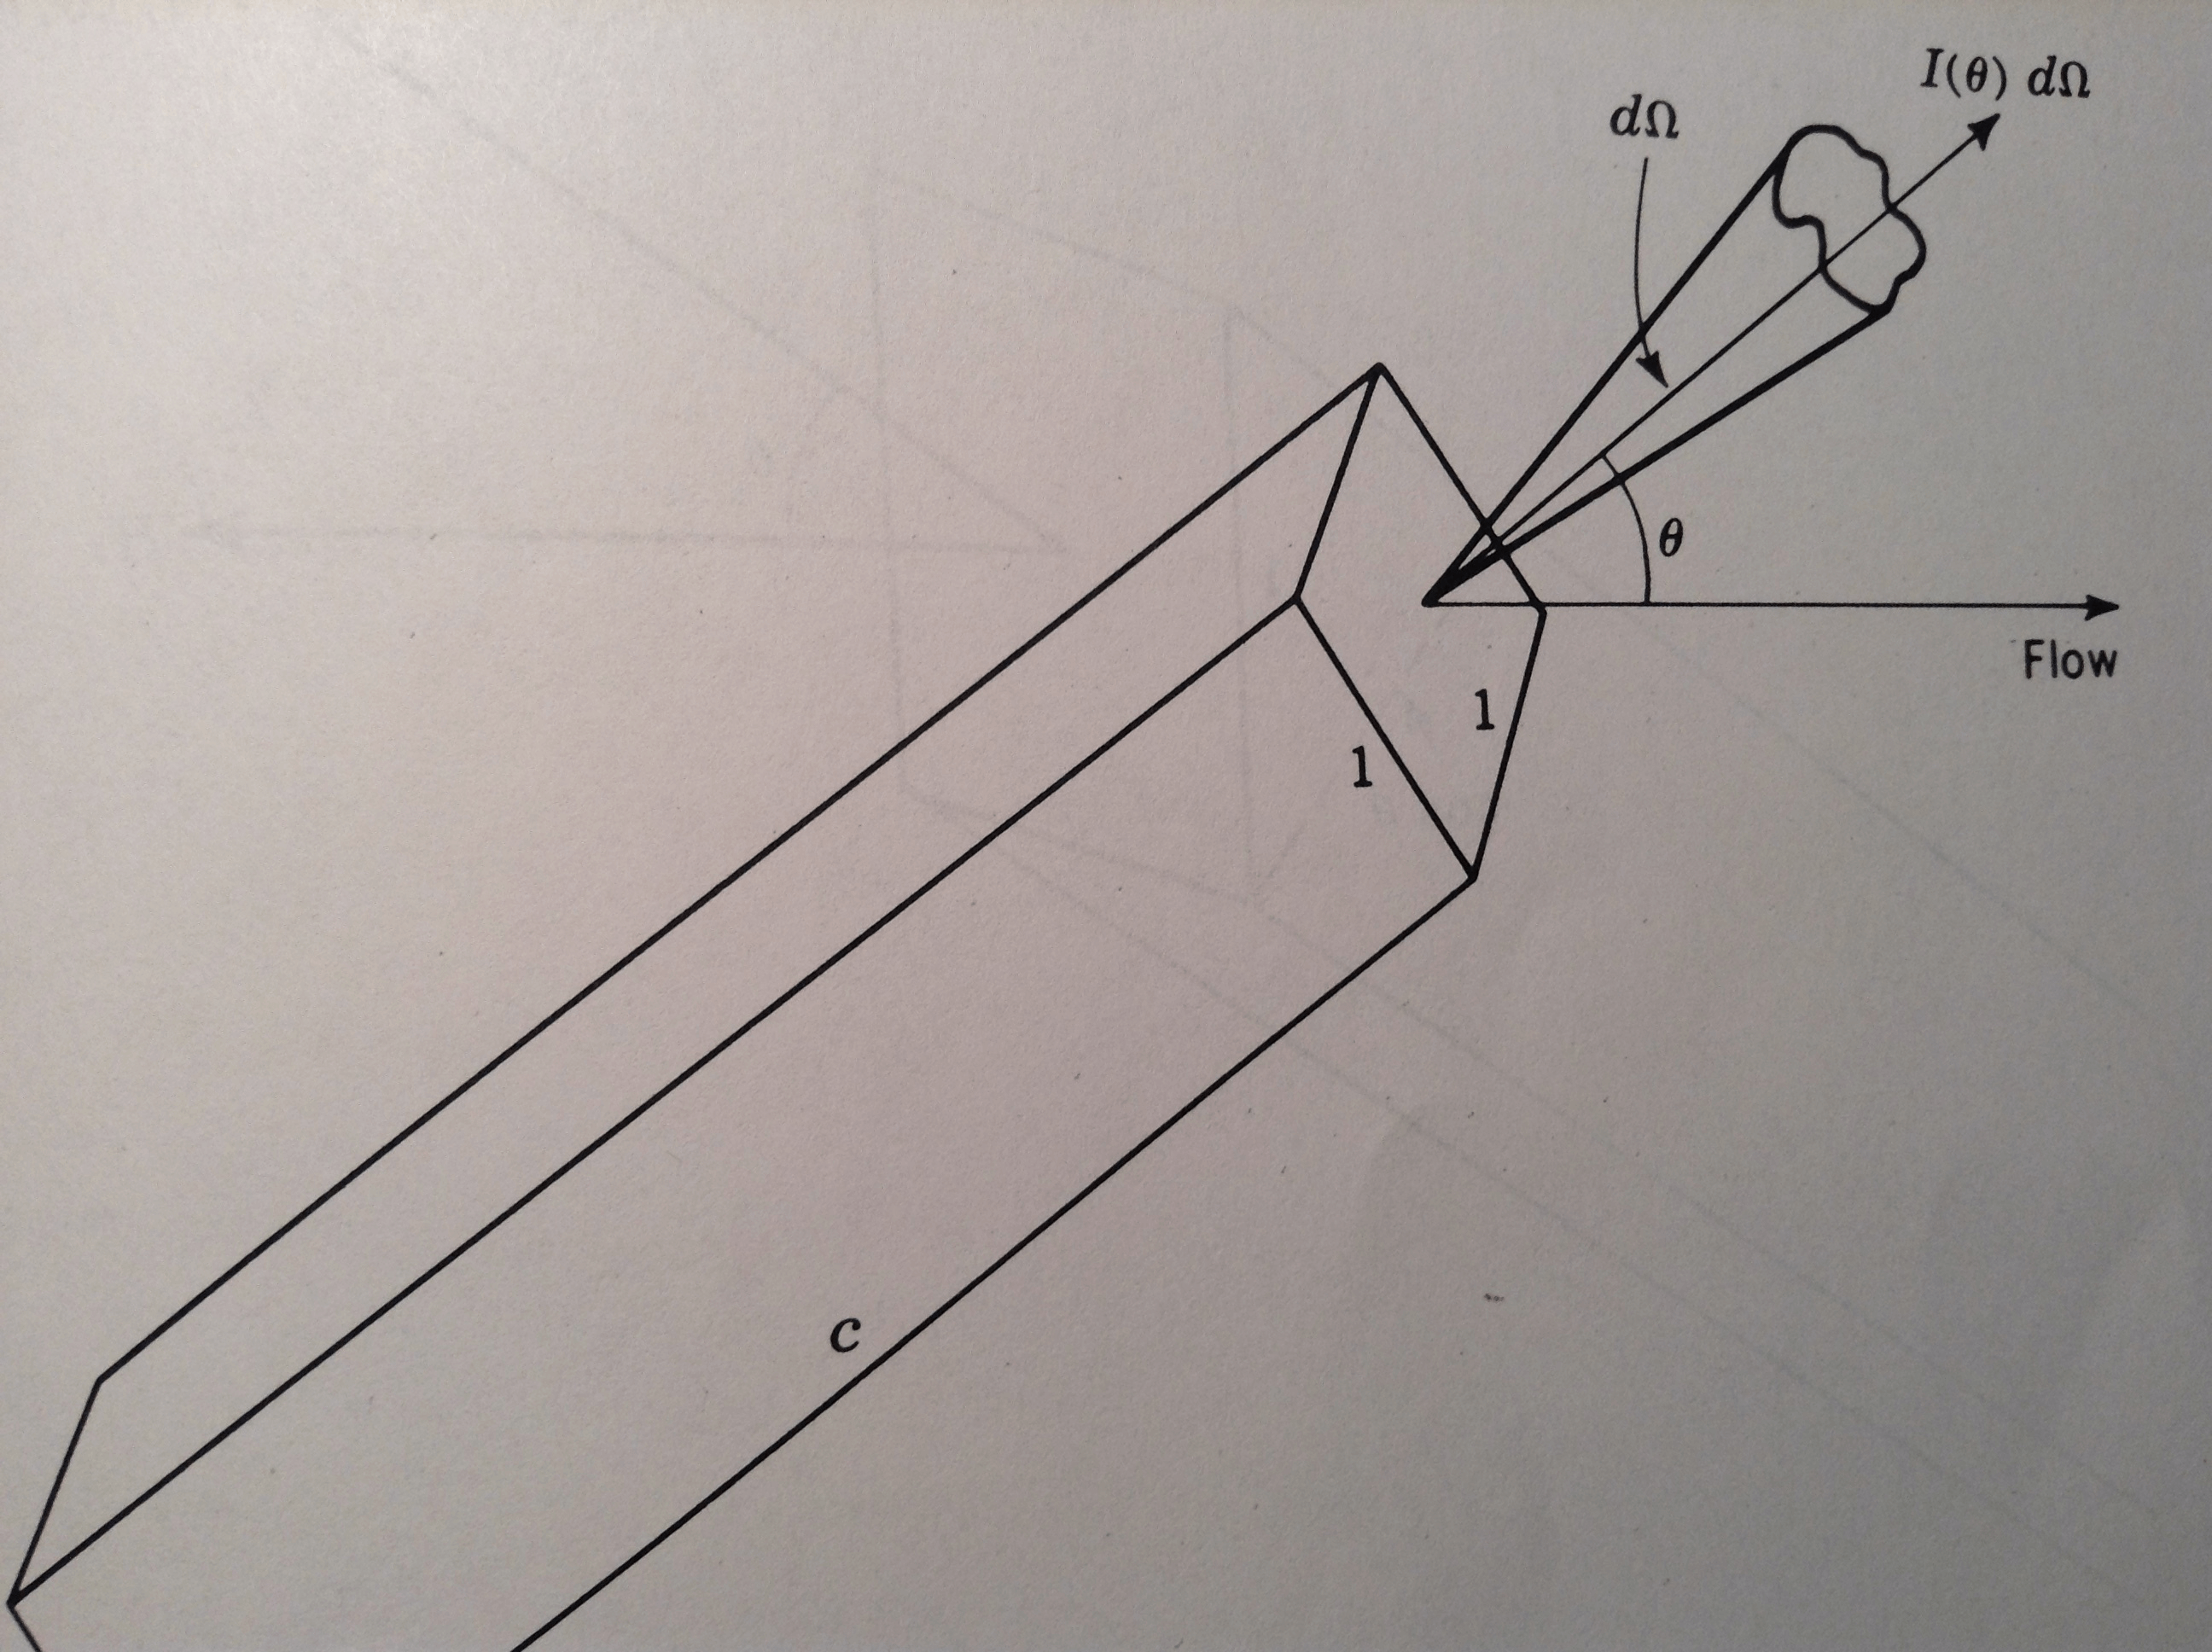
\includegraphics[width=\textwidth,height=0.9\textheight,keepaspectratio]{intensity}
\caption{$I(\theta)\,d\Omega$ is the energy flux moving in direction $\theta$}\label{fig:energyflux}
\end{figure}

\begin{figure}[!ht]
\centering
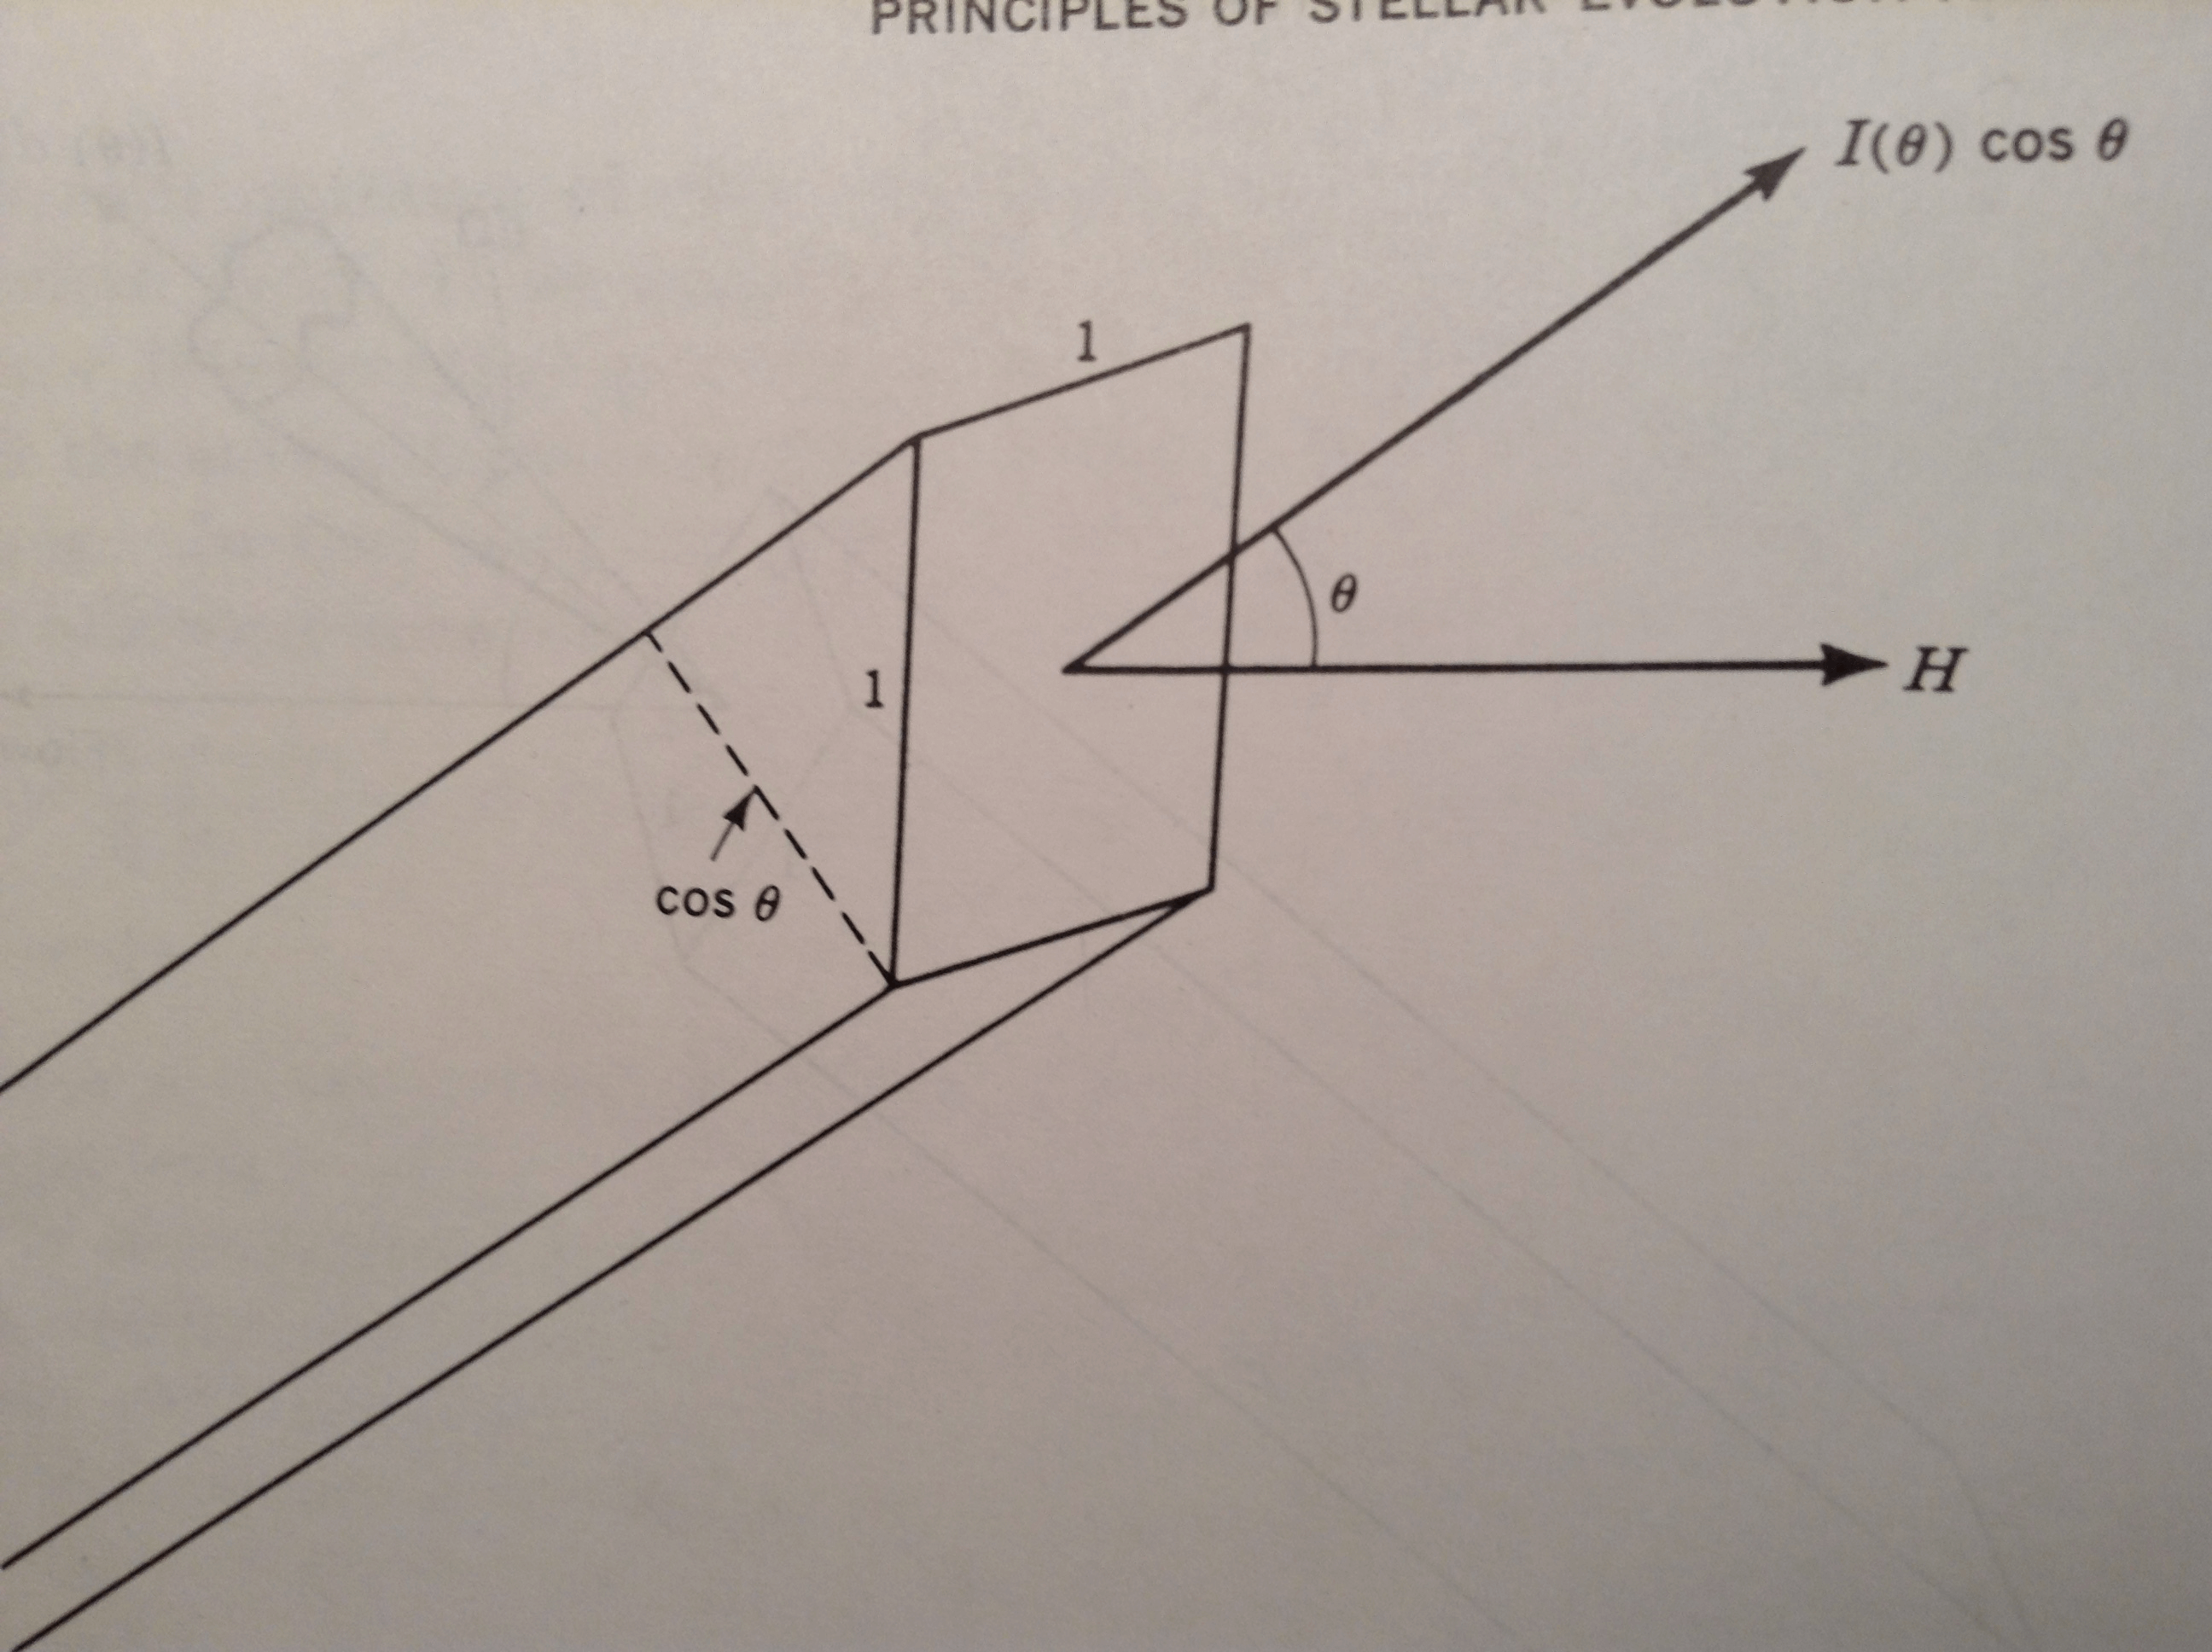
\includegraphics[width=\textwidth,height=0.9\textheight,keepaspectratio]{flux}
\caption{Energy flux with $I(\theta)\,d\Omega$ with associated energy flow per unit area normal to polar axis H equals to $I(\theta)\,d\Omega\cos{\theta}$.}\label{fig:energyflux}
\end{figure}

\begin{figure}[!ht]
\centering
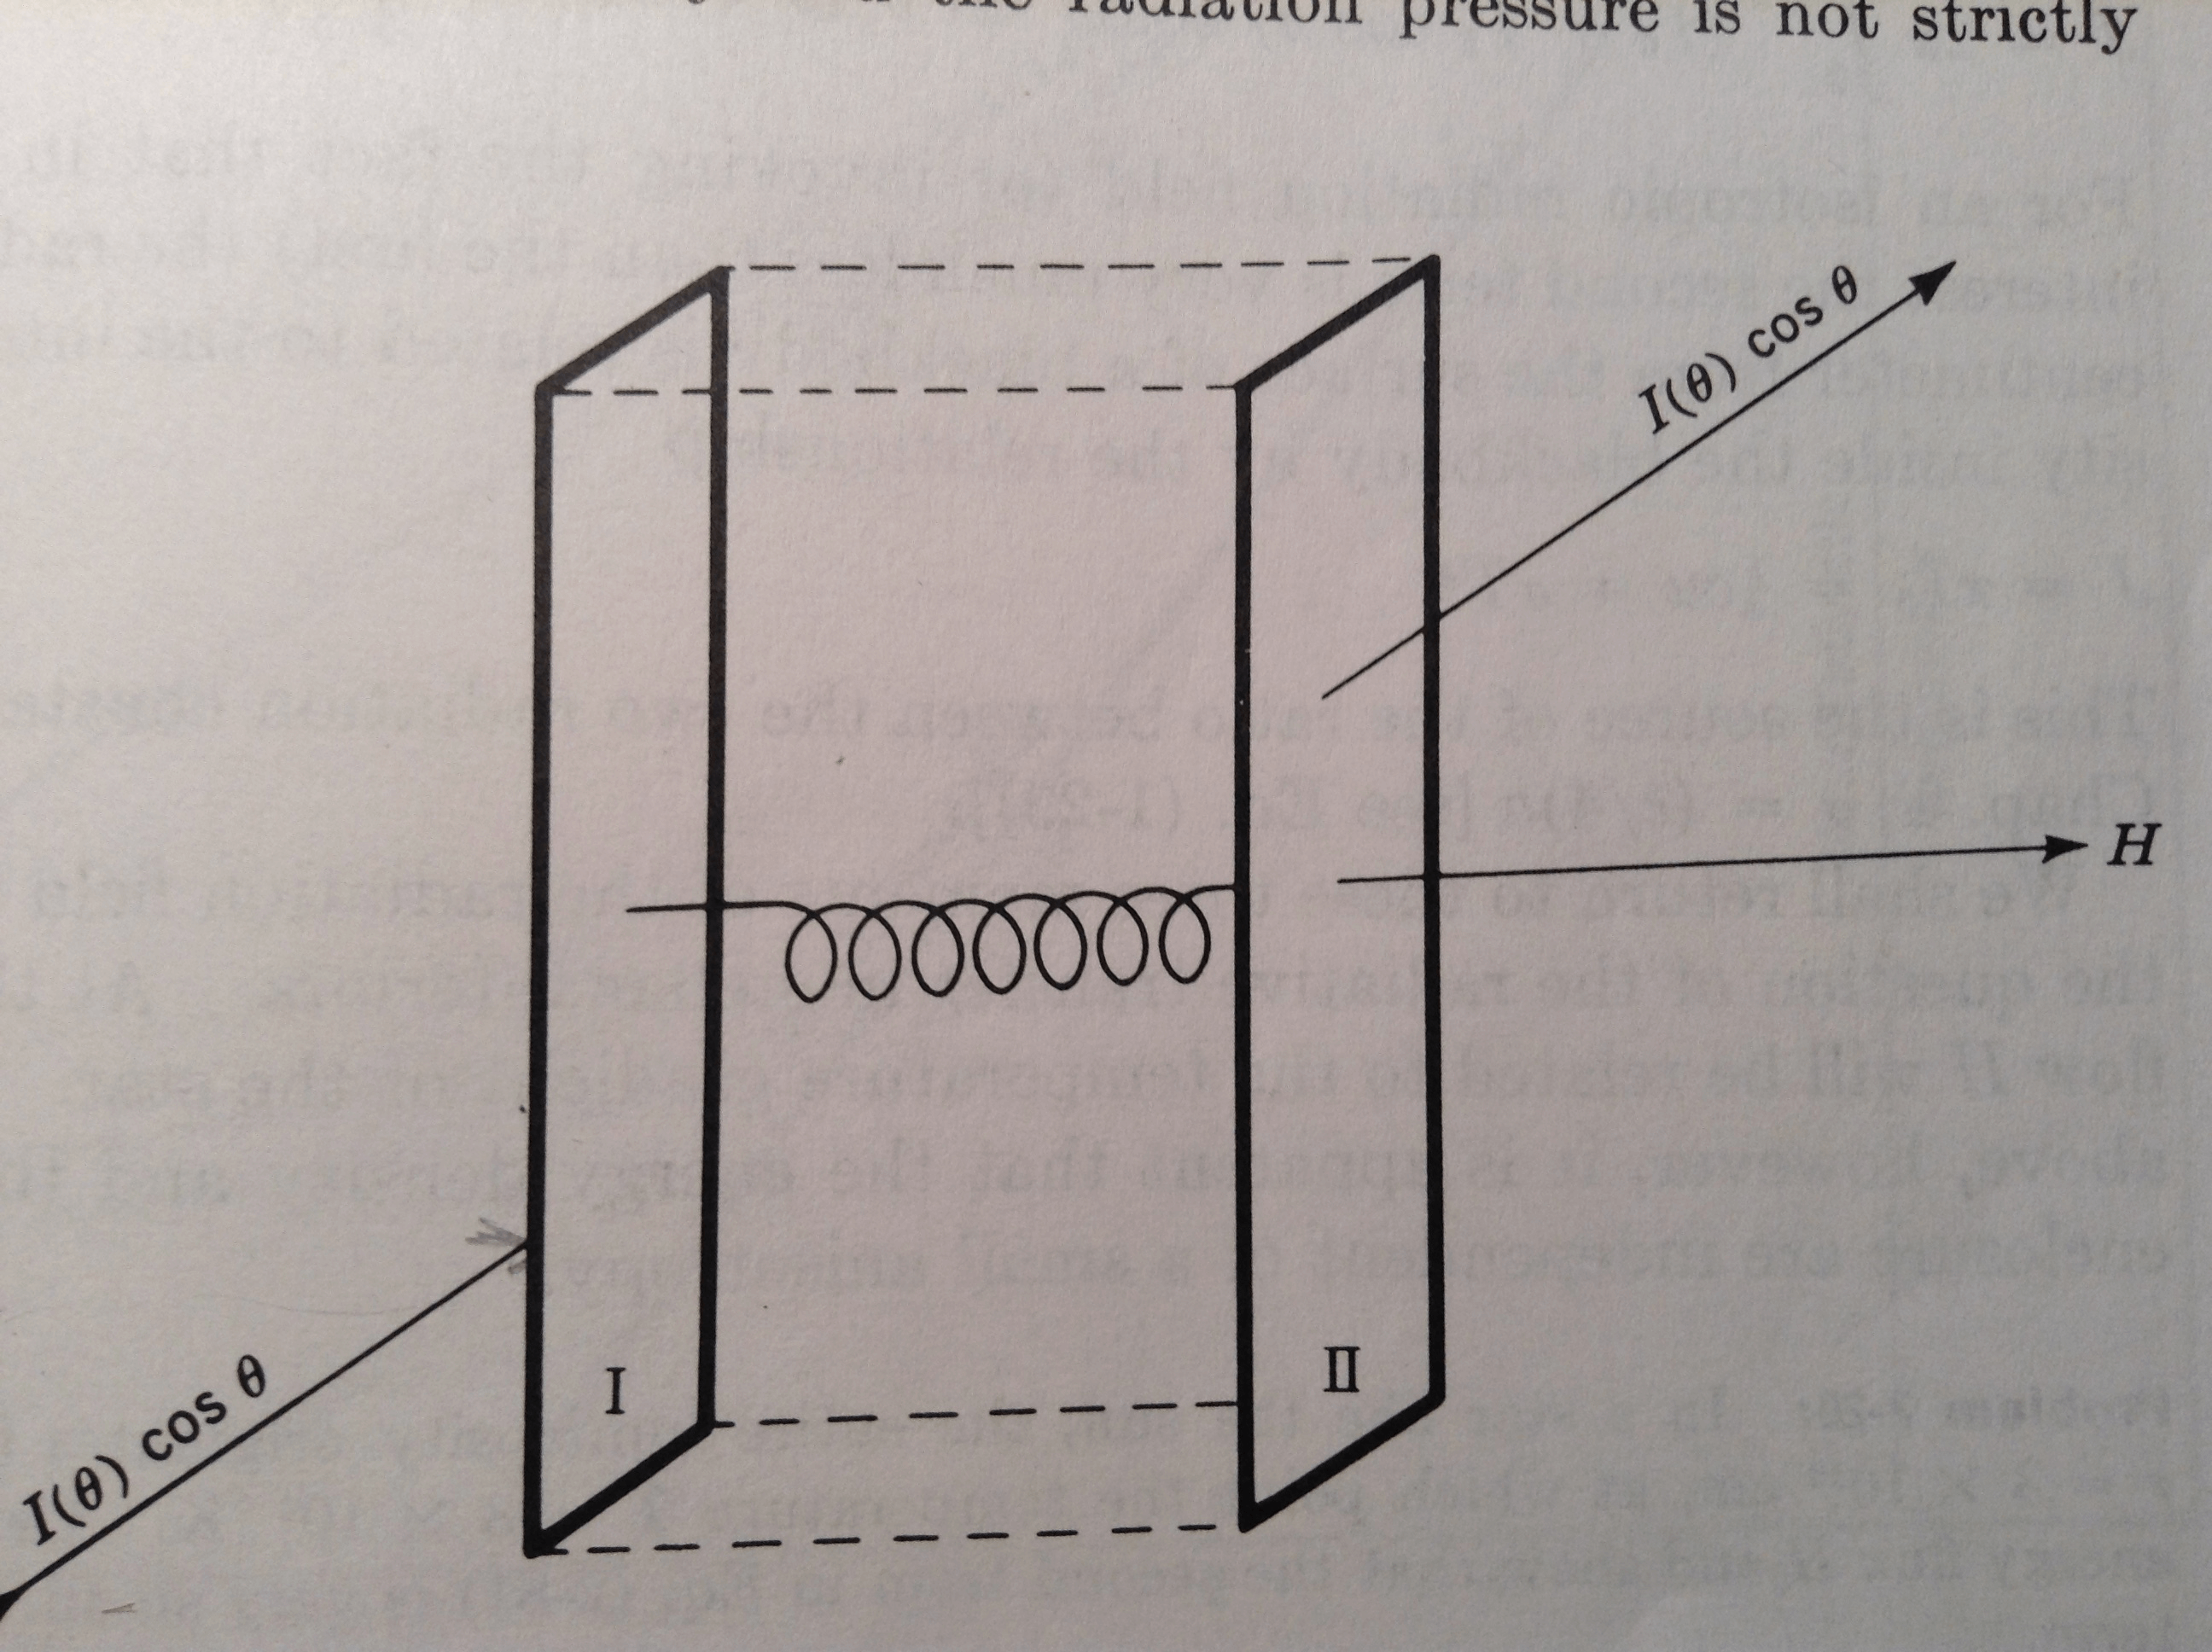
\includegraphics[width=\textwidth,height=0.9\textheight,keepaspectratio]{radpres}
\caption{The radiation pressure is the resulting compressional force on the spring.}\label{fig:radpressure}
\end{figure}

\clearpage

\subsection{Energy flow per unit area in terms opacity and temperature gradient}

\begin{usefull}{A quantity per unit dimension}
Describe characteristic properties of a unitary dimensional entity: mass of unitary surface base cylinder is $\rho\,dl$.
\end{usefull}

What is desired for computation of stellar structure is an equation of transfer that gives energy flow per unit area in terms of an averaged opacity and temperature gradient.

Multiplying the radiative equation transport by $\cos{\theta}$ and dividing by total mass of cylinder of unit area $\rho\,dl$

\begin{align*}
&\frac{1}{\rho}\PDy{r}{I_{\nu}}\cos^2{\theta}\,d\Omega=\frac{1}{\rho}\PDof{r}\int I_{\nu}\cos^2{\theta}\,d\Omega=\frac{c}{\rho}\PDy{r}{P_{\nu}}\\
&\int (\kappa_{\nu a}^*+\kappa_{\nu s})I_{\nu}(r,\theta)\cos{\theta}\,d\Omega=(\kappa_{\nu a}^*+\kappa_{\nu s})H_{\nu}\\
&\int \kappa_{\nu a}^*B_{\nu}(T)\cos{\theta}\,d\Omega=0
&j_{\nu s}=0&\intu{assuming p contains only even power of cosine between the scattering beams}
\end{align*}

The result of these operations on equation of transfer is

\begin{equation*}
\frac{c}{\rho}\PDy{r}{P_{\nu}}=-(\kappa_{\nu a}^*+\kappa_{\nu s})H_{\nu}(r)
\end{equation*}
even in case of a slightly anisotropy $P_{\nu}=\frac{1}{3}u_{\nu}$. The total heat flux per unit area is
\begin{equation*}
H=\intzi{}H_{\nu}\,d\nu=-\frac{c}{3\rho}\intzi{}\frac{1}{\kappa_{\nu a}^*+\kappa_{\nu s}}\TDy{r}{u_{\nu}}\,d\nu
\end{equation*}

Since $u_{\nu}$ is function only of T in thermodynamic equilibrium \mblock{\TDy{r}{u_{\nu}}=\TDy{T}{u_{\nu}}\TDy{r}{T}}
\begin{align*}
&H=-\frac{c}{3\rho}\intzi{}\frac{1}{\kappa_{\nu a}^*+\kappa_{\nu s}}\TDy{T}{u_{\nu}}\TDy{r}{T}\,d\nu&\intertext{which multiplied/divided by}\\
&\intzi{}\TDy{T}{u_{\nu}}\,d\nu=\TDof{T}\intzi{}u_{\nu}\,d\nu=4aT^3&\intertext{becomes:}\\
&H=-\frac{4ac}{3\rho}T^3\TDy{r}{T}\frac{\intzi{}\frac{1}{\kappa_{\nu a}^*+\kappa_{\nu s}}\TDy{T}{u_{\nu}}\,d\nu}{\intzi{}\TDy{T}{u_{\nu}}\,d\nu}&\intertext{and since in thermodynamical equilibrium $B_{\nu}$ differs from $u_{\nu}$ by a constant we define:}\\
&\frac{1}{\kappa}=\frac{\intzi{}\frac{1}{\kappa_{\nu a}[1-\exp{-\frac{h\nu}{kT}}]+\kappa_{\nu s}}\TDy{T}{B_{\nu}}\,d\nu}{\intzi{}\TDy{T}{B_{\nu}}\,d\nu}
\end{align*}

The correction factor for induced emission diminuisce l'assorbimento a basse energie \mblock{h\nu<kT}, the weighting factor $\TDy{T}{B_{\nu}}$ physically mean that the photon frequencies most important for radiative transfer are those for which the difference in the product of photon number density times photon energy between two points of slighly different T is maximal.

\begin{usefull}{Radiative heat flux in stellar interior}
\begin{equation*}
H=F(r)=\frac{l}{4\pi r^2}=\frac{4ac}{3\rho\kappa}T^3\TDy{r}{T}
\end{equation*}
\end{usefull}


\subsection{Euristic derivation}
todo

\subsection{Properties of stars in radiative equilibrium}

\begin{align*}
&\TDy{r}{P_r}=-\frac{\kappa\rho}{4\pi cr^2}l(r)\\
&\TDy{r}{l(r)}=4\pi r^2\rho\epsilon\\
&\TDy{P}{P_r}=\frac{\kappa l(r)}{4\pi G m(r)}\\
&\eta(r)=\frac{\overline{\epsilon_r}}{\epsilon}=\frac{l(r)/m(r)}{L/M}\\
&\TDy{P}{P_r}=\frac{L}{4\pi cGM}\kappa\eta\\
&P_r(r)=\frac{L}{4\pi cGM}\int_0^{P(r)}\kappa(r)\eta(r)\,dP\\
&=\frac{L}{4\pi cGM}P(r)\overline{\kappa\eta}
\end{align*}


\begin{usefull}{Ratio of radiation pressure to total pressure}
The ratio of radiation pressure to total pressure at a point inside a star in radiative equilibrium is proportional to averaged value of $\kappa\eta$ for regions exterior to point r anfd the average is taken by $p(r)$.

\end{usefull}

\begin{usefull}{Luminosity formula}
For stellar center
\begin{align*}
&\beta_c=\frac{P_g}{P}\\
&L=\frac{4\pi cGM(1-\beta_c)}{\overline{\kappa\eta}}
\end{align*}
\end{usefull}

\begin{usefull}{Standard model: non-degenerate polytrope of index 3}
Constant $\beta$ yield the non degenerate polytrope of index 3
\begin{align*}
&P=K\rho\expy{\frac{n+1}{n}}\\
&P_g=\frac{N_ak}{\mu}\rho T=\beta P,\ P_r=\frac{1}{3}aT^4=(1-\beta)P\\
&T=(\frac{N_ak}{\mu}\frac{3}{a}\frac{1-\beta}{\beta})\rho\expy{\frac{1}{3}}&\intu{closure relation??}\\
&P=K\rho\expy{\frac{4}{3}}&\intertext{constancy of $\beta$ depends on constancy of $\kappa\eta$: $\kappa$ increases by several order of magnitude from center to surface and $\eta$ decreases by several order of magnitude}\\
&
\end{align*}
\end{usefull}

\begin{usefull}{Mass-luminosity relationship for main-sequence stars}
\begin{align*}
&T_c\propto M\expy{\frac{2}{3}}\overline{\rho}\expy{\frac{1}{3}}=\frac{M}{R}\\
&\TDy{r}{T}\propto\frac{T_c}{R}\\
&L\propto R^2\frac{(M/R)^3}{M/R^3}\frac{M/R}{R}=M^3
\end{align*}
\end{usefull}

\section{Radiative energy transport.}

\subsection{Mean-free path of a photon.}

\begin{align*}
&l_{Ph}=\frac{1}{\kappa\rho}&\intertext{$\kappa$ is a mean absorption coefficient: Radiative cross section per unit mass averaged over frequency $(\kappa\approx1\,cm^2/g)$. Per il sole:}\\
&l_{Ph}^{\odot}=2\,cm\ll\rsun&\intertext{$\uparrow$ con $\rhosun=\frac{3\msun}{4\pi\rsun^3}=14g/cm^3$. Stellar matter is very opaque.}
\end{align*}

\subsection{Stefan-Boltzman law.}

L'energia interna in una corpo nero di volume V \'e $U=Vu(T)$ dove $u(T)$ \'e la densit\'a di energia dei fotoni:
\begin{align*}
&\frac{du}{u}=4\frac{dT}{T}\\
&u=aT^4
\end{align*}


\subsection{Radiation pressure}

Tutte le volte che un atomo emette/assorbe un fotone perde/guadagna quantit\'a di moto e dato che un atomo emette in maniera isotropa il momento netto \'e nullo una volta mediato su molte emissioni.

I processi di assorbimento non sono isotropicamente distribuiti dato il flusso uscente di energia per $cm^2$ per sec F: solo una frazione $\kappa$ del flusso di momento $\frac{F}{c}$ \'e assorbita dalla materia. Il trasferimento da parte della radiazione di momento alla materia per $cm^3$ per sec, cio\'e la forza esercitata dalla radiazione \'e $\kappa H \frac{1}{c}$.

Un elemento di volume $dS\,dr$ subisce per effetto dell'assorbimento della radiazione una variazione d'impulso $dq$, nel caso un fotone venga assorbito la variazione del flusso uscente \'e $dF<0$

The distribution of photons over over different quantum states with energies $\epsilon_k=\hbar\omega_k$ (large volume $\omega_k\to\omega$) 
\begin{align*}
\overline{n_k}=\frac{1}{\exp{\frac{\hbar\omega}{KT}}-1}
\end{align*}

Moltiplicando il numero di stati nel dato range di frequenze per la distribuzione di Plank (numero di occupazione) ottengo il numero di fotoni e l'energia radiativa nel range di frequenza

\begin{align*}
&dN_{\omega}=\frac{V}{\pi^2c^3}\frac{\omega^2\,d\omega}{\exp{\frac{\hbar\omega}{KT}}-1}\\
&dE_{\omega}=\frac{V\hbar}{\pi^2c^3}\frac{\omega^3\,d\omega}{\exp{\frac{\hbar\omega}{KT}}-1}
\end{align*}


\begin{align*}
&dq=-(n_{\nu}\,dSc\,dt)*(\kappa\rho\,dr)*\frac{h\nu}{c}&\intertext{Il primo termine \'e il numero di fotoni pasanti per superficie $dS$ in tempo $dt$, il secondo \'e la probabilit\'a d'assorbimento attraverso spessore $dr$, il terzo \'e la quantit\'a di moto di ogni fotone.}\\
&dP_r=\TDy{S}{F}=\TDof{S}\TDy{t}{q}\\
&=-\int \,d\nu n_{\nu}c\kappa_{\nu}\rho\,dr\frac{h\nu}{c}\\
&F_{\nu}=n_{\nu}ch\nu,\\
&\TDy{r}{P(Rad)}=-\int\,d\nu\frac{F(Rad)}{c}\kappa_{\nu}\rho&\intertext{In condizioni di LTE posso confrontare $\uparrow$ con}\\
&P_{\nu}=\frac{1}{3}u_{\nu},\ P(Rad)=\frac{1}{3}aT^4&\intertext{e ricavare il gradiente di temperatura necessario per il flusso di energia $F(Rad)$:}\\
&\TDy{r}{T}=-\frac{3\kappa\rho l(r)}{16\pi acT^3r^2}
\end{align*}


\subsection{Local thermodynamic equilibrium}


The thermodynamic theory of radiation is valid only when system is adiabatically enclosed (all parts at same temperature): many physical system though they aren't in thermodynamic equilibrium yet they permit introduction of a temperature to describe local properties: if $\kappa_{\nu}$, $j_{\nu}$ are the coefficient of absorption emission of an element mass we have




\section{Radiative transport: photon diffusion.}


\subsection{Stima del gradiente di temperatura: Local thermal equilibrium.}

Close to local thermal equilibrium
\begin{equation*}
\frac{\Delta T}{\Delta r}\approx\frac{T_c-T_0}{R}|_{\odot}\approx1.4\sci{-4}\,K/cm
\end{equation*}

The radiation field at a given point is emitted from a small nearly adiabatic surrounding:
\begin{align*}
&\Delta T\approx l_{Ph}(\TDy{r}{T})\approx3\sci{-4}K&\intertext{Relative anisotropy of radiation with $T=\sci{7}\,K$:}\\
&\frac{\Delta u}{u}\approx\frac{4T^3\Delta T}{T^4}=\frac{4\Delta T}{T}\approx\sci{-10}
\end{align*}

\subsection{Diffusion of Radiative energy.}

The radiation in stellar interior is very close to that of a black body but the small anisotropy carries the huge luminosity of star:

$\sci{-10}$ of the flux emitted from $1 cm^2$ of a black body at $T=\sci{7}K$ is $\sci{3}$ times larger than flux at solar surface ($6\sci{10}\,erg/cm^2/s$).

Radiative transport occurs because of surplus of outgoing radiation emitted by hotter marial below over the ingoing radiation emitted from less hot material above.

Since $l_{Ph}\ll\rsun$ radiative transport in stars can be treated as a diffusion process

\begin{align*}
&\vec{J}=-D\nabla n&\intertext{$\uparrow$ is the flux (diffusive) of particles per unit area per unit time between places of different particles densities,}\\
&D=\frac{1}{3}vl_P&\intertext{is the diffusion coefficient determined by mean velocity and mean free path of particles.}\\
&|F|=\frac{1}{3}cl_{Ph}\PDy{r}{u},\quad\PDy{r}{u}=4aT^3\PDy{r}{T}&\intertext{$\uparrow$  ipotesi di simmetria sferica}\\
&F=-\frac{4ac}{3}\frac{T^3}{\kappa\rho}\PDy{r}{T}&\intertext{$\uparrow$ can be interpeted as heat conduction equation $F=-k_{Rad}\nabla T$. Ricavo il gradiente di T sostituendo $l=4\pi r^2F$:}\\
&\PDy{r}{T}=-\frac{3}{16\pi ac}\frac{\kappa\rho l(r)}{r^2T^3}\\
&\PDy{m}{T}=-\frac{3}{64\pi^2 ac}\frac{\kappa l(r)}{r^4T^3}&\intertext{$\uparrow$ these equations become invalid when one approaches the surface: $l_{Ph}$ becoms large (Large optical depth $d\tau=\rho\kappa\,dr$: stellar interior).}
\end{align*}

\subsection{Rosseland mean for opacity}

Considero la dipendenza dalla frequenza per radiazione $[\nu,\nu+\,d\nu]$

\begin{align*}
&F_{\nu}=-D_{\nu}\nabla U_{\nu},\quad D_{\nu}=\frac{1}{3}cl_{\nu}=\frac{c}{3\kappa_{\nu}\rho}\\
&u_{\nu}=\frac{4\pi}{c}B(\nu,T)=\frac{8\pi h}{c^3}\frac{\nu^3}{\exp{\frac{h\nu}{KT}}-1}&\intertext{B is the Plank function for intensity of black body radiation}\\
&\vec{F}=-[\frac{4\pi}{3\rho}\int_0^{+\infty}\frac{1}{\kappa_{\nu}}\PDy{T}{B}\,d\nu]\nabla T&\intertext{Definisco la media di Rosseland tramite:}\\
&\frac{1}{\kappa}=(\underbrace{\frac{acT^3}{\pi}}_{\int_0^{\infty}\PDy{T}{B}\,d\nu})^{-1}\int\frac{1}{\kappa_{\nu}}\PDy{T}{B}\,d\nu&\intertext{The rosseland mean favours the frequency ranges of maximum energy flux:}\\ &F_{\nu}=-(\frac{1}{\kappa_{\nu}}\PDy{T}{B})\frac{4\pi}{3\rho}\nabla T\\
&\kappa_{\nu}=X\kappa_{\nu}(H)+Y\kappa_{\nu}(He)&\intertext{$\uparrow$ opacity for given frequency for mixture of H and He.}
\end{align*}


\subsection{Stability condition for radiative equilibrium}

Consider the perturbation: I displace an element of matter in stellar interior upward by the distance $dr$, let's the element expand adiabatically until the pressure inside the element is in balance with the pressure of the surroundings.

\begin{figure}[!ht]
\centering
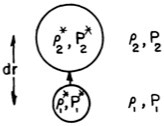
\includegraphics[width=(0.3\textwidth),height=(\textheight-11mm),keepaspectratio]{conv_stab}
\caption{Perturbation of radiative layer to test for stability against convection.}
\end{figure}

After the perturbation the density may differs now from that of the surroundings since internal density is determined by adiabatic transformation of the element
\begin{align*}
P_2=P_2^*,\quad\rho_2^*=\rho_1^*(\frac{P_2^*}{P_1^*})^{\frac{1}{\gamma}}&\intertext{where $\gamma=\frac{c_P}{c_v}$ is the ratio of specific heat and has the value $\frac{5}{3}$ for highly ionized gas}
\end{align*}

The pressure force exerted on that volume which the element occupies after its displacement and expansion has not be alterated by the perturbation, the gravitational force will be altered if the density within the element after the perturbation differs from that in the surroundings.

Condizione di stabilit\'a
\begin{align*}
\rho_2^*>\rho_2&\intertext{I can trasform this condition in a more practical one: sobstituting expression for the variables of surroundings and taking taylor's expansion of the quantities at higher position:}\\
-\frac{1}{\gamma}\frac{1}{P}\TDy{r}{P}<-\frac{1}{\rho}\TDy{r}{\rho}
\end{align*}

For the cases where the equation of state for an ideal gas hold I can take logarithimic derivative of $P=\frac{k}{\mu}\rho T$ and thus I can express density gradient in terms of temperature and pressure gradient:

\begin{align*}
-(1-\frac{1}{\gamma})\frac{T}{P}\underbrace{\TDy{r}{P}}_{\text{from HE}}>-\underbrace{\TDy{r}{T}}_{\text{from RE}}&\intertext{since both temperature gradient and pressure gradient are negative both sides of $\uparrow$ are positive. Right side contains absolute value of temperature gradient, left side contains the adiabatic temperature gradient (would represent temperature gradient if the temperature and pressure followed the adiabatic relationship through the layer).}
\end{align*}

For a layer to be stable against convection the actual temperature gradient must be lower in absolute value than the adiabatic temperature gradient.\index{Stability condiction against convection: Schwarzschild.}

The above condiction hold only in homogenous layers.


\section{Meccanismi che contribuiscono  all'opacit\'a.}

\subsection{Radiation and equilibrium}

\begin{definition}{Emission coefficient.}
\begin{align*}
&j_{\nu}=m\,d\omega\,dt\,d\nu&\intu{amount of radiant energy emitted: $j_{\nu}$ is the emission coefficient for frequency $\nu$.}
\end{align*}
\end{definition}

\begin{definition}{Einstein coefficients.}
\begin{itemize}
\item Spontaneous emission.

The probability that in a interval of time $dt$ an atom in an excited state n emits a quantum of energy $h\nu_{mn}$ in the solid angle $d\omega$ in absebce of external field is $A_{nm}\,d\omega\,dt$: this spontaneous emission take place uniformly in all direction.

\item Stimulated emission.

The probability that an excited atom in state n is stimulated by external field of radiation to emit a quantum $h\nu_{nm}$, in the direction $d\omega$, in time $dt$ is given by $B_{nm}I_{\nu_{nm}}\,d\omega\,dt$, where $I_{\nu_{nm}}$ is the intensity of radiation of frequency $\nu_{nm}$ at the point where the atom is located and in the direction $d\omega$: the induced emission of radiation by a given pencil of radiation take place in the same direction as incident pencil.

\end{itemize}

In condizioni di equilibrio termodinamico
\begin{equation*}
j_{\nu}=\kappa_{\nu}B_{\nu}(T)
\end{equation*}
where T is the (local) temperature.

If there are $N_m$ atoms in n-th state per unit volume
\begin{align*}
&\frac{A_{nm}}{B_{nm}}=\frac{2h\nu_{nm}^3}{c^2}\\
&\frac{N_mB_{mn}}{N_nB_{nm}}=\exp{\frac{h\nu_{nm}}{KT}}
\end{align*}

\end{definition}

Vedi Chandrasekhar pg 190

\subsection{Electron scattering.}

Lo scattering da parte di un elettrone di un'onda EM incidente ovvero, l'emissione di dipolo di un'elettrone oscillante indotta da un'onda elettromagnetica \'e equivalente all'assorbimento del fotone:
\begin{align*}
&\sigma_e=\frac{8\pi}{3}(\frac{e^2}{m_ec^2})^2=\SI{6.652e-25}{\square\cm}&\intu{Thomson cross-section, the associated opacity coefficient is due to combined effect of all electrons in a unit mass of gas}\\
&\kappa_{es}=\frac{\sigma_e}{\frac{\rho}{n_e}}=\frac{\sigma_e}{\mu_em_u}&\intertext{for totally ionized gas $\mu_e=\frac{2}{1+X}$:}\\
&\kappa_{es}=0.20(1+X)\si{\square\cm\per\gram}
\end{align*}

Electon scattering is important source of opacity in ionized gas not too dense. When degree of ionization drops ($T\leq\SI{e4}{\kelvin}$, in H-rich gas) the electron density become so small that  $\kappa_{es}$ is strongly reduced.

\subsubsection{Energetic photons: Effetto Compton.}

When photon energy becomes significant fraction of rest mass of electron $h\nu\geq0.1m_ec^2$ the exchange of momentum between photon and electron must be taken in account (Compton scattering): at high temperature since maximum of Plank function is at \mblock{h\nu=4.965 KT,\ KT\geq0.02m_ec^2} or $T\geq\SI{e8}{\kelvin}$: At high temperature the electron scattering opacity is reduced.

\subsection{Free-free absorption.}

A free electron cannot absorbs a photon because of momentum/energy conservation; it can happens if there is an EM with a close ion: it's the inverse process of bremsstrahlung. The derivation of absorption coefficient is a QM problem: an approximate calculation is the Kramer's law.

\subsubsection{Kramer's law.}

The absorption efficiency of the temporary electron-ion system is proportional to $Z_i^2\nu^{-3}$

\begin{align*}
&\kappa_{\nu}^{ff}\propto\frac{n_e}{\rho}\sum_in_iZ_i^2T\expy{-\frac{1}{2}}\nu^{-3}&\intu{cross-section of ion i:}\\
&\overline{v}=\sqrt{\frac{3KT}{m_e}}\\
&\Delta t\propto1/\overline{v}\propto T\expy{-\frac{1}{2}}&\intu{time of effective ion-electron coupling.}\\
&\sigma^{ff}_i\propto n_eT\expy{-\frac{1}{2}}Z_i^2\nu\expy{-3}&\intertext{the opacity coefficient follows by multiplying $\uparrow$ by $\frac{n_i}{\rho}$.}\\
\end{align*}

In a completely ionized gas $\frac{n_e}{\rho}=\frac{1}{\mu_em_u}=\frac{1+X}{2m_u}$.

\begin{align*}
&\kappa_{ff}\propto\rho T\expy{-\frac{7}{2}}\\
&\kappa_{ff}\propto\num{3.8e22}\rho T\expy{-\frac{7}{2}}\si{\square\cm\per\gram}
\end{align*}

We have to the into account of QM effects with the Gaunt factor.

\subsection{Bound-free, bound-bound absorption.}

\begin{itemize}
\item Bound-free absorption is the absorption of a photon by a bounded electron where the photon energy exceed ionization energy $\chi$. Classical consideration lead to formula of the Kramer form.
\item Bound-Bound absorption. Efficient because the absorption lines are broadened by collisions. Important for $T\leq\SI{e6}{\kelvin}$.
\item Bound-free absorption of negative hydrogen ion ($\chi=\SI{0.75}{\ev}$). Important in cool stars or solar atmosphere. The resulting opacity is sensitive to metallicity and temperature: the free electrons to make ion come from single ionized metals such as Na, K, Ca, Al.
\item Dust and molecules. In cool stars with $\teff\leq\SI{4000}{\kelvin}$ opacity from molecules and dust grain ($T\leq\SI{1500}{\kelvin}$) becomes dominant.
\end{itemize} 

\subsubsection{Negative H ion}

\subsection{Temperature-density diagram for the opacity.}

\begin{todo}{Temperature-density diagram for the opacity}
Schwarzschild pg 67-73
\end{todo}

\begin{figure}[!ht]
\centering
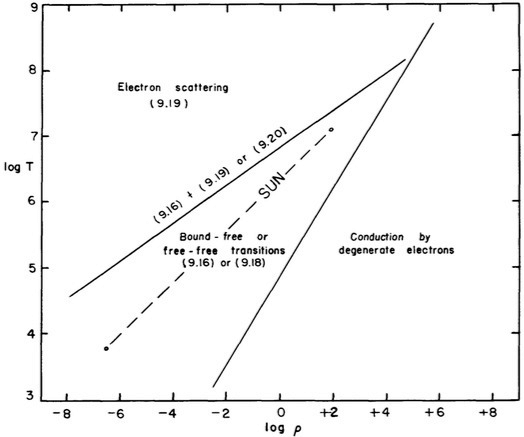
\includegraphics[width=(0.9\textwidth),height=(\textheight-11mm),keepaspectratio]{kappaqu}
\caption{Temperature-density diagram for the opacity.}
\end{figure}

\clearpage

\section{Relazione Massa-Luminosit\'a}

\subsection{Stability of thermal equilibrium}

Estimate of luminosity in the sun midway between center and surface.

\begin{align*}
&L_r=4\pi r^2\frac{4ac}{3}\frac{T^3}{\kappa\rho}\TDy{r}{T}&\intertext{$\uparrow$ radiative equilibrum plus crude estimates:}\\
&\kappa\rho\approx1cm,\quad T\approx10\sci{6}\,K&\intertext{taking for differnetial the difference I have:}\\
&L\approx6\sci{35}&\intertext{$\uparrow$ exceeds the luminosity of the sun by a factor 100.}
\end{align*}

How does the luminosity of a star depends on its mass?

\begin{align*}
&L_r=4\pi r^2\frac{4ac}{3}\frac{T^3}{\kappa\rho}\TDy{r}{T}&\intertext{$\uparrow$ radiative equilibrum plus crude estimates:}\\
&\rho\propto \frac{M}{R^3}&\intertext{introducing this proportionality in hydrostatic equilibrium equation $\downarrow$}\\
&\TDy{r}{P}=-\frac{Gm(r)\rho}{r^2}&\intertext{we find the dependence of representative pressure on the mass and radius $\downarrow$}\\
&P\propto\frac{M^2}{R^4}&\intertext{from equation of state for ideal gas, $T\propto\frac{P}{\rho}$, we have $\downarrow$}\\
&T\propto\frac{M}{R}&\intertext{introducing the proportinalities for T and P in radiative equilibrium equation we obtain:}\\
L\propto M^3
\end{align*}

\index{Mass-Luminosity relation: radiative equilibrium condition.}

The above estimates point out that the luminosity of a star is not determined by the rate of energy generation by nuclear process: only radiative equilibrium condition enters in the derivation.

The pressure force must counteract gravity according to HE equation: if the pressure have to be high enough for this porpuse the internal temperature must have certain relatively high values according to equation of state. The temperature gradient from hot internal zone to cold surface will cause a net radiation flux according to 
\begin{equation*}
l(r)=-4\pi r^2\frac{4ac}{3}\frac{T^3}{\kappa\rho}\TDy{r}{T}
\end{equation*}

The stength of this radiation flux will be fixed by radiative equilibrium condition irrespective of whether or not the the energy loss is compensate by nuclear energy production in the interior. If the energy loss by radiation at the surface is bigger the nuclear energy generation the suffers a net energy loss: this can made up from gravitational energy by contraction. During the contraction one half of the gravitational energy is available for radiation losses from surface, the other half go into increase of thermal energy. The contraction will stops when the over-all rate nuclear energy release is equal to radiative surface losses.


\subsection{Relazione massa luminosit\'a: limite di Eddington.}

Ipotesi:
\begin{itemize*}
\item Trasporto in superficie \'e radiativo conduttivo
\item $\kappa$ \'e approx costante
\item La pressione di radiazione fornisce un contributo dominante alla pressione totale
\end{itemize*}

Se la pressione di radiazione fornisce un contributo dominante $P\approx P_r$ ho
\begin{align*}
&\TDy{r}{P_r}=-\frac{\kappa_{\nu}}{c}\rho\frac{l(r)}{4\pi r^2}&\intertext{$\uparrow$ LTE}\\
&\PDy{r}{P}\approx\PDy{r}{P_r}=-\frac{Gm(r)\rho}{r^2}&\intertext{$\uparrow$ equilibrio idrodinamico}\\
&L=l(R)=GM\frac{4\pi c}{\kappa}&\intertext{Stimo il valore della costante di proporzionalit\'a fra massa e luminosit\'a nel caso di stelle massicce $\beta=\frac{P_g}{P}\approx0$:}\\
&\frac{L}{\lsun}\approx\sci{4}\frac{M}{\msun}&\intertext{$\uparrow$ \'e un limite superiore: limite di Eddington. Utile per studio dei nuclei galatticci. Utilizzando il modello di Eddington ($\beta=const$) invece ho:}\\
&\TDy{r}{P_r}=(1-\beta)\TDy{r}{P}=-(1-\beta)\frac{Gm(r)}{r^2}\rho&\intertext{quindi}\\
&L\approx[1-\beta(M)]\sci{4}(\frac{M}{\msun})\lsun&\intertext{Per piccole masse $\beta\approx1$ e quindi $1-\beta(M)\propto M^2$ ho:}\\
&L\propto M^3
\end{align*}

\subsection{Tempo di vita per oggetti che si avvicinano al limite di Eddington}

Energia disponibile
\begin{align*}
E_d=\alpha Mc^2&\intertext{$\alpha\approx0.01$ per reazioni nucleari, $\alpha\approx1$ per oggetti massicci.}
\end{align*}

Stimo il tempo di vita sulla base dell'energia disponibile
\begin{align*}
&T_{Max}=\frac{E_d}{L}\approx\frac{\alpha Mc^2}{\sci{4}M\lsun/\msun}=\alpha T_0\\
&=\alpha*(2\sci{9}\,yr)
\end{align*}


\section{Conductive transport of energy}

\subsection{Conduction in ordinary stellar matter}

In ordinary stellar matter conduction has no chance of taking over an appreciable part of the total energy transport.

Although the small collisional cross section for particles of ionized gas the large density result in a $l_{gas}$ several orders of magnitude smaller than $l_{ph}$ and velocities are few percent of c.

\subsection{Conduction in degenerate stellar interior}

In the core of evolved stars where the electron gas is highly degenerate conduction becomes efficient. Gli elettroni sono pi\'u vicini all'energia di Fermi e poich\'e le celle dello spazio delle fasi sono piene le collisioni in seguito a cui cambia il momento sono improbabili: il coefficiente di diffusione aumenta.

\subsection{Heat transfer equation}

\begin{align*}
&\PDy{m}{l}=\epsilon-\PDy{t}{u}+\frac{P}{\rho^2}\PDy{t}{\rho}&\intertext{$\uparrow$ equation of local energy equilibrium. Sostituisco in $\uparrow$ le espressioni $\downarrow$:}\\
&l=-\sigma^*\PDy{m}{T},\quad u=c_vT&\intertext{quindi}\\
&\PDof{m}(\sigma^*\PDy{m}{T})-c_v\PDy{t}{T}=-[\epsilon+\frac{P}{\rho^2}\PDy{t}{\rho}]&\intertext{se pongo il lato destro uguale a zero ho un'equazione che ha la forma dell'equazione di trasporto di calore con conducibilit\'a $\sigma^*$. nel caso di un problema unidimensionale ho}\\
&\PDof{x}(\sigma\PDy{x}{T})=c\PDy{t}{T}&\intertext{La soluzione di $\uparrow$ con le condizioni al bordo tende alla soluzione costante dopo un tempo sufficiente:}\\
&T(x,t)\to T(x)=const
\end{align*}

Timescale of thermal adjustment.

\begin{align*}
&\tau_{Adj}=\frac{c}{\sigma}d^2&\intertext{Eqution of heat transfer demand the characterisc time $\uparrow$ with d is a characteristic lenght over which the initially given $T(x)$ function changes. For a star (\mblock{\PDof{m}\to\frac{1}{M}}, \mblock{L\approx\frac{\sigma^*\overline{T}}{M}}):}\\
&\tau_{Adj}=\frac{c_vM^2}{\overline{\sigma^*}}\ \Rightarrow \ L=\frac{E_i}{T}=\frac{\overline{\sigma}^*\overline{T}}{M}
\end{align*}

Nel caso di stelle degeneri
\begin{align*}
&\tau_{Adj}\approx\frac{c_v\overline{T}M}{L}=\frac{E_i}{L}=\tkh&\intertext{$\uparrow$ when energy is efficiently transported by conduction.}
\end{align*}


\section{Radiative equilibrium. Eddington luminosity.}

\subsection{Radiation pressure gradient}

Il trasporto radiativo implica un gradiente di temperatura non nullo e quindi un gradiente della pressione di radiazione dato da

\begin{align*}
&\TDof{r}(P_{Rad})=\TDof{r}(\frac{1}{3}aT^4)=\frac{4}{3}aT^3\TDy{r}{T}\\
&=-\frac{\kappa\rho}{4\pi c}\frac{l}{r^2}&\intertext{Radiation pressure gradient represents an outward force due to net flux of photons.}
\end{align*}

\subsection{Upper limit to local luminosity}

For a star in hydrostatic equilibrium the outward radiation force must be smaller than the inward force of gravity as given by pressure gradient necessary for HE

\begin{align*}
&|\TDy{r}{P_{Rad}}|<|(\TDy{r}{P})_{HE}|\quad\Rightarrow\quad\frac{\kappa\rho}{4\pi c}\frac{l}{r^2}<\frac{Gm\rho}{r^2}\\
&l<\frac{4\pi cGm}{\kappa}=l_{Edd}\index{Luminosit\'a di Eddington}&\intertext{$\uparrow$ is the max luminosity that can be carried by radiation inside a star in HE}\\
\end{align*}

\subsection{Convective energy transport}

The Eddington limit for local luminosity of a star can be violated in case of very large flux (as for intense nuclear burning) or in case of very high opacity (outer layers of the sun: rel. low T near the ionization temperature of H and He). In such cases hydrostatic equilibrium and radiative equilibrium can't hold together, therefore if the star is to remains in HE energy must be transported by different mean than radiative diffusion: convection, the collective motion of gas bubbles that carry heat and can distributes it efficiently.

\subsection{Necessary condition for stability against convection}

\begin{align*}
&L<L_{Edd}=\frac{4\pi GM}{\kappa}&\intertext{For the surface of a star:}\\
&L_{Edd}=3.8\sci{4}(\frac{M}{\msun})(\frac{0.34cm^2/g}{\kappa})\lsun&\intertext{$\uparrow$: $\kappa$ is the opacity of photosphere, $0.34cm^2/g$ correspond to electron scattering opacity for $X=0.7$.}
\end{align*}


\subsection{Stability condition for radiative equilibrium: relation between convection criterion and Eddington limit.}

If we want construct a stable model of a star every layers of the star must have such properties that every small fluctuation is smeared away. That is pressure gradient must be computed from hydrostatic equilibrium condition $\TDy{r}{P}=-g(r)\rho=-\rho G\frac{m(r)}{r^2}$, the temperature gradient from the radiative equilibrium condition $l(r)=-4\pi r^2\frac{4ac}{3}\frac{T^3}{\kappa\rho}\TDy{r}{T}$ and both gradients have to be inserted in the condition dynamical stability

\begin{equation*}
-(1-\frac{1}{\gad})\frac{T}{P}\TDy{r}{P}>-\TDy{r}{T}
\end{equation*}

To relate the convection criterion for stability, $\nrad{}<\nad{}$ (\sch{} criterion) with $\nrad{}=(\TDly{P}{T})_{Rad}=\frac{3}{16\pi acG}\frac{\kappa lP}{mT^4}$ temperature gradient if the entire energy flux is transported by radiation, to the Eddington limit we write $\nrad{}$ in terms of $l$ and $l_{Edd}=\frac{4\pi cGm}{\kappa}$ and $P_{Rad}=(1-\beta)P$:

\begin{align*}
l<4(1-\beta)\nad{}l_{Edd}&\intertext{$\uparrow$ \sch{} criterion in terms of $l$ and $l_{Edd}$. For $\beta>0$ and $\nad{}>0.25$ convection sets in before Eddington limit is reached.}
\end{align*}


\section{$(L,M,R)$ relations.}

\subsection{Maximum mass for main sequence stars. }

In very luminous main-sequence stars the opacity is dominated by electron scattering. I can assume $\kappa$ constant.

\begin{align*}
L_{Edd}\propto M&\intertext{while for stars (at least in the main sequence: $x\approx3.5$)}\\
L\propto M^x,\quad x>1&\intertext{We can expect a maximum mass for main-sequence stars.}
\end{align*}

\index{Mass-luminosity relationship: limite superiore per sequenza principale}


\subsection{Rough estimate of Mass-Luminosity relationship.}

Estimate of luminosity in the sun midway between center and surface.

\begin{align*}
&L_r=4\pi r^2\frac{4ac}{3}\frac{T^3}{\kappa\rho}\TDy{r}{T}&\intertext{$\uparrow$ radiative equilibrum plus crude estimates:}\\
&\kappa\rho\approx1cm,\quad T\approx10\sci{6}\,K&\intertext{taking for differnetial the difference I have:}\\
&L\approx\num{6e35}&\intertext{$\uparrow$ exceeds the luminosity of the sun by a factor 100.}
\end{align*}

How does the luminosity of a star depends on its mass?

\begin{align*}
&L_r=4\pi r^2\frac{4ac}{3}\frac{T^3}{\kappa\rho}\TDy{r}{T}&\intertext{$\uparrow$ radiative equilibrum plus crude estimates:}\\
&\rho\propto \frac{M}{R^3}&\intertext{introducing this proportionality in hydrostatic equilibrium equation $\downarrow$}\\
&\TDy{r}{P}=-\frac{Gm(r)\rho}{r^2}&\intertext{we find the dependence of representative pressure on the mass and radius $\downarrow$}\\
&P\propto\frac{M^2}{R^4}&\intertext{from equation of state for ideal gas, $T\propto\frac{P}{\rho}$, we have $\downarrow$}\\
&T\propto\frac{M}{R}&\intertext{introducing the proportinalities for T and P in radiative equilibrium equation we obtain:}\\
L\propto M^3
\end{align*}

\index{Mass-luminosity relationship (Rough)}

\subsection{LL e C}


\chapter{Dynamical instability. Convective energy transport.}
\PartialToc

\section{Dynamical instability}

\subsection{Small fluctuation in concentric shell}

Until now we have supposed perfect spherical symmetry: all function and variables are constant on a concentric sphere. In reality will arise small fluctuations on such a sphere: these local perturbation may be ignored if it don't grow.

In the basic equations spherical symmetry can be kept if we interpret the variables as a proper average over a concentric sphere. 

\subsection{Local description for the stability of a layer: mass elements and average surroundings.}

In local description we represent a fluctuation by mass element $(e)$ in which the functions have constant but somewhat different values then in the average surroundings

\begin{figure}[!ht]
\centering
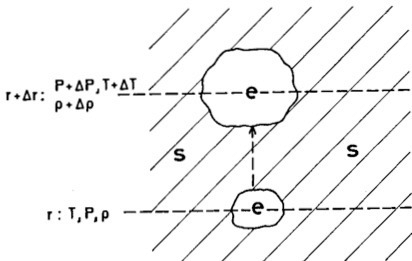
\includegraphics[width=(0.6\textwidth),height=(\textheight-11mm),keepaspectratio]{esconv}
\caption{Test of stability of a layer.}
\end{figure}

We suppose that the moving elements have no time to exchange appreciable amlount of heat with the surroundings: adiabatic movement (Dynamical instability).

Difference between the element and surroundings
\begin{equation*}
DA=A_e-A_s
\end{equation*}

\begin{itemize*}
\item For $DP\neq0$ expansion/contraction occurs at sound speed: much more rapid than other motions of elements.

We can suppose $DP=0$.

\item Let's suppose an initial fluctuation in T, $DT>0$: $DT>0$ requires that, for ideal gas ($\rho\propto\frac{P}{T}$), $D\rho<0$: the element is lighter than surroundings material, temperature fluctuations are accompained by radial local motion.

\item Let's suppose a radial displacement $\Delta r$
\begin{align*}
&D\rho=[(\TDy{r}{\rho})_e-(\TDy{r}{\rho})_s]\Delta r&\intertext{the terms in squares are change in density of the element while rises $dr$ minus spatial gradient of the surroundings}
\end{align*}

A finite $D\rho$ gives the radial component \mblock{K_r=-gD\rho} of a buoyancy force per unit of mass (g is the gravity acceleration): if $D\rho<0$ the perturbation is increased by the $K_r>0$

\end{itemize*}

Convection instability leads to cyclic macroscopic motion but the star is still in overall hydrostatic equilibrium.

\section{Condition for stability for radial fluctiations.}

\subsection{Condition for stability: density gradient}

For a radial upward fluctiation of an element:

if $D\rho<0$ the element is lighter and $K_r>0$, the situation is unstable.

If $D\rho>0$ the $K_r<0$: the element is drawn back to its original position: the layer is stable.

\begin{align*}
&(\TDy{r}{\rho})_e-(\TDy{r}{\rho})_s>0&\intertext{$\uparrow$ is highly impractical}
\end{align*}

\subsection{Condition for stability: temperature's and mean molecular weight's gradient}

\begin{align*}
&\frac{d\rho}{\rho}=\alpha\frac{dP}{P}-\delta\frac{dT}{T}+\phi\frac{D\mu}{\mu}&\intertext{with the coefficients:}\\
&\alpha=\Dcvar{\PDly{P}{\rho}}{T,\mu},\   \delta=\Dcvar{\PDly{T}{\rho}}{P,\mu},\\ &\phi=\Dcvar{\PDly{\mu}{\rho}}{T,P}&\intertext{For ideal gas:}\\
&\rho\propto\frac{P\mu}{T},\quad \alpha=\delta=\phi=1, d\mu_e=0\\
&-(\frac{\delta}{T}\TDy{r}{T})_e+(\frac{\delta}{T}\TDy{r}{T})_s-(\frac{\phi}{\mu}\PDy{r}{\mu})_s>0&\intertext{}
\end{align*}

\subsection{Scale height of pressure}

\begin{align*}
&H_P=-\frac{dr}{d\,\ln{P}}=-P\frac{P}{r}\\
&H_P=\frac{P}{\rho g}, \quad \PDy{r}{P}=-g\rho&\intertext{$H_P$ has the dimension of a length and its value represents the characteristic scale of radial pressure variation.}\\
&\parbox{1.3cm}{Solar photosphere:}\left\{\begin{array}{c}
g=2.7 \sci{4}\,cm\,s^{-2} \\
P=6.8\cdot\sci{4}\,dyn\,cm^{-2}\\
\rho=1.8\sci{-7}\,g\,cm^{-3}\\
\end{array}\right.\\
&\Rightarrow H_P=1.4\sci{7}\,cm\\
&r=\frac{\rsun}{2}:\ \left\{\begin{array}{c}
g=1.0 \sci{5}\,cm\,s^{-2} \\
P=6.7\cdot\sci{14}\,dyn\,cm^{-2}\\
\rho=1.3\,g\,cm^{-3}\\
\end{array}\right.\\
&\Rightarrow H_P=5.2\sci{9}\,cm
\end{align*}

\subsection{Condition for stability: adiabatic Temperature gradient (\sch{}).}

Anticipo il criterio di \sch{} di \ref{ssec:schcstab}.

Abbiamo visto che piccole fluttuazioni radiali di quantit\'a di materia di uno strato sferico di una stella (per esempio spostamento vero l'alto) avvengono in equilibrio di pressione con gli strati attraversati dalla porzione di materia:

The expansion of the gas element as it rises $\Delta r$ occurs on the local dynamical timescale (with  the speed of sound) and therefore the displacement and expansion of the gas element will be very close to adiabatic.

\begin{align*}
\frac{\delta P_e}{P_e}=\gamma_{Ad}\frac{\delta \rho_e}{\rho_e}&\intertext{$\gamma_{Ad}$ is the adiabatic exponent:}\\
\gamma_{Ad}=(\TDly{\rho}{P})_{Ad}\\
\TDly{P}{\rho}>\frac{1}{\gamma_{Ad}}&\intertext{$\uparrow$ criterion for stability against convection: the density gradient must be steeper than a critical value determined by $\gamma_{Ad}$}
\end{align*}

\begin{figure}[!ht]
\centering
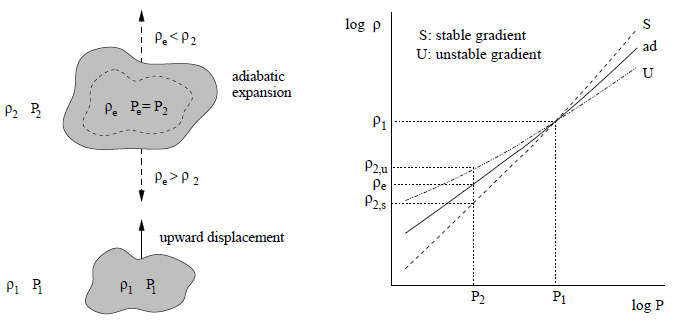
\includegraphics[width=(\textwidth),height=(\textheight-11mm),keepaspectratio]{acvsadTgrad}
\caption{A layer is stable against convection if the density varies more steeply with pressure than for an adiabatic change.}
\end{figure}

\clearpage

\section{Condiction for stability against convection: Ledoux, Schwarzschild criteria}

The following criteria to test the stability of layers against convection are local ones: easily evaluated at given place given local $P$, $T$, $\rho$ only.
\index{Local criteria for convection stability}
In extreme cases the local forces must be coupled to the neighbouring layers by momentum transfer, inertia continuity equation.

\subsection{General condition for stability: use of pressure scale height}

\begin{align*}
H_P[-(\frac{\delta}{T}\TDy{r}{T})_e+(\frac{\delta}{T}\TDy{r}{T})_s-(\frac{\phi}{\mu}\TDy{r}{\mu})_s]>0
\end{align*}

\subsection{Ledoux's criterion}

Riscrivo il criterio di stabilit\'a per fluttuazioni radiali in forma simbolica

\begin{align*}
&\underbrace{(\TDly{P}{T})_s}_{\nabla}<\underbrace{(\TDly{P}{T})_e}_{\nabla_e}+\frac{\phi}{\delta}\underbrace{(\TDly{P}{\mu})_s}_{\nabla_{\mu}}&\intertext{$()_s$ are both spatial derivatives in which P is taken as a measure of depth, $\nabla_e$ is the variation of T in the element during the motion (position is measured by P).}\\
&\nablaTact<\nel+\frac{\phi}{\delta}\nmu
\end{align*}

In a layer that transport all energy by radiation $\nablaTact=\nrad$, let's test such a layer for stability. We have supposed adiabatic change for the element fluctuations $\nel=\nad$.
We have the Ledoux criterion for stability of a radiative layer against convection (dynamical stability)

\begin{align*}
\nrad<\nad+\frac{\phi}{\delta}\nmu
\end{align*}

$\nmu\neq0$ in interior of evolving stars where heavier elements are usually produced below the lighter ones: molecular weight increases inward and the relative terms in the stability condition has a stabilizing effect ($\delta$, $\phi$ are positive).

\subsection{Schwarzschild's criterion}\label{ssec:schcstab}

In regions with homegenous chemical composition $\nmu=0$.
We have the Schwarzschild criterion for the stability of a radiative layer

\begin{align*}
\nrad<\nad
\end{align*}

\subsection{Causes of instability}

According to Schwarzschild criterion convection occurs when $\nrad=\frac{3}{16\pi acG}\frac{P}{T^4}\frac{\kappa l}{m}>\nad$.

Zones where we may found convective instability
\begin{itemize*}

\item Opaque region of stars: large value of $\kappa$. For example in outer regions of the Sun because opacity increses with decreasing temperature. Since low mass stars are cooler than high mass stars we may expect the former to have convective envelopes.

\item Regions with a large value of $\frac{l}{m}$ are regions with large energy flux. Toward the center of a star $\frac{l}{m}\approx\epsilon_{nuc}$: stars with nuclear energy production strongly peaked toward the center can be expected to have a convective core. That is the case of massive stars. 

\item We can have small values of $\nad$ in the zones of partial ionization of H and He at relatively low temperature and, even if the opacity is small the surface layers of stars may be unstable against convection. Stars of all masses have  shallow surface  convection zones at temperatures where lighter elements are partially ionized.

\end{itemize*}

\subsection{Convective zones in $\msun$ and $4\msun$ stellar model.}

\begin{figure}[!ht]
\centering
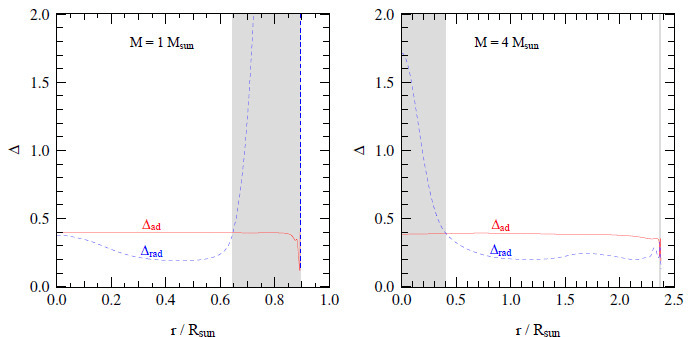
\includegraphics[width=(0.9\linewidth),keepaspectratio]{shallowconv}
\caption{Variation of $\nad$ and $\nrad$ with radius in two models at the start of main sequence.}
\end{figure}

In both models $\nad\approx0.4$ since conditions are close to an ideal gas, in the surface ionization zones $\nad<0.4$ and a thin convective layer appears in the $4\msun$ model.

The solar mass model has a very large opacity in its outer layer, resulting in a large value of $\nrad$ which gives rise to convective envelope where $\nrad>\nad$ (gray shading).

The $4\msun$ model has a hotter outer envelope with lower opacity so that $\nrad$ stay small; the large energy generation rate in the center result in a convective core.

\clearpage

\subsection{Sketch of temperature gradients}

For an unstable layer violating the \sch{} criterion we can plot the different gradients: in a $\ln{P}-\ln{T}$ diagram an adiabatic change follows a line with slope $\nad{}$, the changes in a rising element are given by $\nel{}$, while the stratifications in the surroundings and in a radiative layer are shown by lines with slopes $\nablaTact{}$ and $\nrad{}$ respectively.

Suppose $\nmu{}=0$ it follows from the violation of genaral condition for dynamic stability in the general case

\begin{equation*}
\nablaTact<\nel+\frac{\phi}{\delta}\nmu
\end{equation*}
that is $\nablaTact{}>\nel{}$. If some part of the flux is carried by convection then $\nablaTact{}<\nrad{}$ (that is to say if the entiere energy flux would be transported by radiation the actual T gradient would be greater).

Let's consider a rising element starting from $(P_0,T_0)$: this element moves downward to the left corner along the line with slope  $\nel{}$. Since $\nablaTact{}>\nel{}$, the element, although cooling, will have an increasing temperature excess over its new surroundings: it will radiates energy into its surroundings which means that the element cools more than adiabatically: $\nel{}>\nad{}$.\index{"Super-adiabatic" cooling}

\begin{align*}
\nrad{}>\nablaTact{}>\nel{}>\nad{}&\intertext{The fact that element's temperature gradient must always be between adiabatic and surroundings temperature gradients shows that the Ledoux and \sch{} criteria are also to be used in near-surface regions where the rising elements lose much of their energy by radiation:}\\
\nrad{}<\nel{}<\nad{}&\intertext{$\uparrow$ for a convective stable layer where $\nel{}>\nad{}$.}
\end{align*}

\begin{figure}[!ht]
\centering
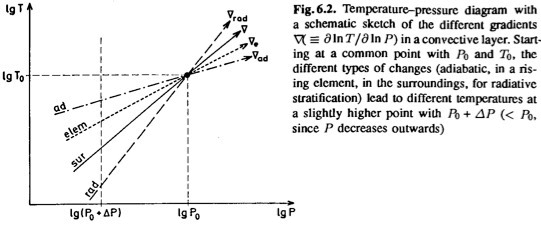
\includegraphics[width=(\textwidth),height=(\textheight-11mm),keepaspectratio]{Tgrads}
\caption{Temperature-pressure diagram with a schematic sketch of the different gradients in convective unstable layer.}
\end{figure}

\clearpage


\section{Oscillation of displaced elements}

\subsection{Equation of motion for mass elements in dynamically stable layers}

In a dynamically stable layer mass elements can oscillate around the equilibrium position because of fluctuations. Consider $\Delta r>0$

\begin{align*}
&D\rho=\frac{\rho\delta}{H_P}[\nel{}-\nablaTact{+\frac{\phi}{\delta}}\nmu{}]\Delta r&\intertext{$\uparrow$ excess of density. Remembering:}\\
&\delta=-(\PDly{T}{\rho}),\ \phi=-(\PDly{\mu}{\rho}),\\ &H_P=-\frac{dr}{d\ln{P}}=-P\TDy{P}{r}\\
&\nablaTact{}=\nablaTacte{},\ \nel{}=\nele{},\\
&\nmu{}=\nmue{}
\end{align*}

In presence of gravity acceleration g the buoyancy force per unit volume is
\begin{align*}
&K_r=-gD\rho&\intertext{producing an acceleration of the element}\\
&\PtwoDy{t}{\Delta r}=-\frac{g\delta}{H_P}[\nel{}-\nablaTact{}+\frac{\phi}{\delta}\nmu{}]\Delta r&\intertext{the righthand side is negative since in a stable layer $\frac{D\rho}{\Delta r}>0$ and thge solution of the equation of motion is of the form}\\
&\Delta r=\Delta r_0\exp{i\omega t}&\intertext{$\uparrow$ oscillations around equilibrium position.}
\end{align*}

\subsection{Frequency of oscillations: the Brunt-V\"ais\"al\"a frequency.}

The frequency of this adiabatic oscillation is the Brunt-\vai{} frequency
\begin{align*}
&\omega^2_{Ad}=\frac{g\delta}{H_P}(\nad{}-\nablaTact{}+\frac{\phi}{\delta}\nmu{})&\intertext{in unstable layers $\omega^2<0$.}
\end{align*}

\subsection{Radiative correction.}\label{ssec:radlosscil}

Suppose $DT>0$, superpose to radial energy flux $\vec{F}$, carrying energy from stellar interior to the surface, there will be a local non-radial flux $\vec{f}$, carrying the surplus energy of the element to its surroundings: the radiative flux from the elements due to its temperature excess will be

\begin{align*}
&f=\frac{4acT^3}{3\kappa\rho}|\PDy{n}{T}|&\intertext{$\PDof{n}$ is differenziation perpendicular to the surface of the element:}\\
&\PDy{n}{T}\approx\frac{2DT}{d}\\
&\lambda=Sf=\frac{8acT^3}{3\kappa\rho}DT\frac{S}{d}&\intertext{$\uparrow$ radiative loss per unit of time from the surface S of the blob, it determines the rate by which the thermal energy of the blob of volume V changes:}\\
&-\lambda=\rho Vc_P\PDy{t}{T_e}\approx\rho Vc_P\PDy{t}{DT}\\
&\PDof{t}(DT)=-\frac{DT}{\tau_{Adj}}&\intertext{$\uparrow$ ho introdotto il tempo caratteristico $\tau_{Adj}$ che \'e approx l'eccesso di calore diviso la luminosit\'a:}\\
&\tau_{Adj}=\frac{\rho Vc_P DT}{\lambda}=\frac{\kappa\rho^2c_Pd^2}{16acT^3}&\intertext{for large elements far from regions of marginal stability:}\\
&\tau_{Adj}\gg\frac{1}{\omega_{Ad}}
\end{align*}

Radiative loss gives a small deviation from adiabatic oscillations.

\section{Mixing length theory}

\subsection{Convective equilibrium}

Let's consider a layer in which the stability condition ($\downarrow$) is not fulfilled
\begin{align*}
&-\frac{1}{\gamma}\frac{1}{P}\TDy{r}{P}<-\frac{1}{\rho}\TDy{r}{\rho}\\
&-(1-\frac{1}{\gamma})\frac{T}{P}\TDy{r}{P}>-\TDy{r}{T}
\end{align*}

Hence upon the slightest perturbation convective motions will break out throughout the unstable layer: a perturbed element which is displaced upwards will have an internal density lower than the surrounding density, it experiences a net upwards force and will continues its upward motion. Similarly for an element displaced downwards.
Both downward and upward moving elements contribute to a convective energy transport upwards.

Assume initially that the layer is in precarious radiative equilibrium with the radiative flux carrying out the energy produced by nuclear processes.

Now because of instability convective motion break out throughout the layer: convective motions will transport thermal energy from lower levels to upper levels of the layer. Thus the temperature gradient will be reduced by convection and thus will be reduced the radiation flux according to equation for radiative equilibrium and the thus will be reduced also the convective energy flux since a reduction of the excess of the actual temperature gradient over the adiabatic temperature gradient.

The lowering of temperature gradient by convection will continue until the radiation flux and convective flux together fulfill the basic thermal equilibrium condition
\begin{equation*}
\TDy{r}{l(r)}=\epsilon\rho4\pi r^2
\end{equation*}

Thus instability of radiative equilibrium of a layer of a star leads to the state of convective equilibrium.

\subsection{Local flux of energy}

In an unstable layer the total flux is 

\begin{align*}
&F_{Rad}+F_{Con}=\frac{l}{4\pi r^2}=\frac{4acG}{3}\frac{T^4m}{\kappa Pr^2}\nrad{}\\
&F_{Rad}=\frac{4acG}{3}\frac{T^4m(r)}{\kappa Pr^2}\nabla_?&\intertext{part of the flux is transported by convection: $\nabla_?>\nablaTact{}$. I want to deriva an expression for}\\
&F_{Con}=\ldots\downarrow
\end{align*}

\subsection{Mean free path of mass elements: mixing length. Uncertainty.}

The mean free path of mass elements is the mixing length $l_m$ after which they dissolve in surroundings.

Great uncertainty: value of mixing length appropriates for stars. 

In Lab. mixing length is approx the linear size of volume in which convection is observed.

We may suppose the mixing length for stars to be of the order of depth of the convective layer: this could be a gross overestimate for layers in which the density drops by a large factor crossing the layer as is the case when convective instability occurs close to surface.

Uncertainty in mixing length has little consequence for convective zones in deep interior of stars, but introduce noticeable uncertainty when the convective instability occurs just below the photosphere.

\subsection{Excess thermal energy per unit volume. Relation between convective energy transport and temperature gradient.}\label{ssec:convEnT}

Let's determine the temperature excess of a rising element over its surroundings.

\begin{align*}
\delta T=(1-\frac{1}{\gamma})\frac{T}{P}\TDy{r}{P}\,dr-\TDy{r}{T}\,dr=\delta\nabla T\,dr&\intertext{$\uparrow$ difference between the adiabatic temperature change within the element and the actual temperature change in the surroundings, $\delta\nabla T$ is defined as the absolute value of the excess of actual temperature gradient  over the adiabatic temperature gradient. For the relation between $dT$ and $dP$ we use the equation of state for ideal gas and the relation between $P$ and $\rho$ for adiabatic changes.}
\end{align*}

Multiplying the temperature excess for $c_P\rho$ I have the excess of thermal energy per unit volume ($cm^3$):
\begin{align*}
&dq=c_P\,dT-\frac{\delta}{\rho}\,dP&\intertext{we will have a finite $\delta T$ while $dP$ will remain infinitesimal infinitesimal:}\\
&\delta q=c_P\rho\delta\nabla T&\intertext{where $\rho$ convert from unit of mass to unit of volume.}\\
&H=\delta\nabla T\,dr\,c_p\rho v&\intertext{$\uparrow$ Energy flux per $cm^2$ per sec}
\end{align*}

\subsection{Local convective energy flux}

Let's consider a convective element with $DT>0$ 
\begin{align*}
&F_{Con}=\rho vc_PDT&\intertext{$\uparrow$ local flux of energy:  analog to H of previous \ref{ssec:convEnT} ($dr\to\overline{dr}=\frac{l_m}{2}$). I have to consider $vDT$ as the proper mean over the whole concentric sphere.}
\end{align*}

\subsection{Radial buoyancy force. Determination of element mean velocity}\label{ssec:bmeanvelocity}

In our(\sch{}) notation $dr$ stands for average displacement (vertical distance from level at which the element had the same temperature as the surroundings): same equations hold for downward displacement $dr<0$ ($v<0$). $v$ is taken to be overall vertical velocity of all elements at one level.


I have to determine v from dynamical consideration
\begin{align*}
&\delta \rho=-\frac{1}{\gamma}\frac{\rho}{P}\TDy{r}{P}\,dr+\TDy{r}{\rho}\,dr&\intertext{$\uparrow$ deficiency of density}\\
&\delta\rho g(r)=&\intertext{$\uparrow$ excess force upward,  deficiency in gravitational force.}
\end{align*}

In more explicit form (with confusing notation $DT\leftrightarrow\delta T$): the elements passing the sphere of radius r will have different $v$ (and $DT$) and the perturbation started with $DT_0\approx0$ and $v_0\approx0$,we assume that the average element has moved $\frac{l_m}{2}$.
I average $vDT$ on the entire sphere of radius $r$.

\begin{align*}
&\frac{DT}{T}=\frac{1}{T}\PDy{r}{(DT)}\frac{l_m}{2}=(\nablaTact{}-\nel{})\frac{l_m}{2}\frac{1}{H_P}\\
&\frac{D\rho}{\rho}=-\delta(\frac{DT}{T})&\intertext{$\uparrow$ is the density difference between element and surroundings and derives from the equation of state}\\
&\frac{d\rho}{\rho}=\alpha\frac{dP}{P}-\delta\frac{dT}{T}+\phi\frac{d\mu}{\mu},\  DP=0=Du&\intertext{with}\\
&\delta=-\Dcvar{\PDly{T}{\rho}}{P}=\frac{T}{v}\Dcvar{\PDy{T}{v}}{P}\\
&K_r=-g\frac{D\rho}{\rho}&\intertext{$\uparrow$ radial buoyancy force per unit mass.}
\end{align*}

I will determine the work done by the excess force on the element: is this work which produces the kinetic energy of the element. Taking the linear approximation I have that the work done over the path between $r$ and $r+\,dr$ (integral of force excess over the path), and putting $\overline{dr}=\frac{l_m}{2}$, is 
\begin{align*}
&\frac{1}{2}K_r\frac{l_m}{2}=g\delta(\nablaTact{}-\nel{})\frac{l_m^2}{8H_P}&\intertext{Let's suppose one-half of this work $\uparrow$ goes into kinetic energy of the element $\frac{v^2}{2}$ (per unit mass) and the other half is transferred which have to be pushed aside:}\\
&v^2=g\delta(\nablaTact{}-\nel{})\frac{l_m^2}{8H_P}&\intertext{$\uparrow$ gives convection velocity as a function of temperature gradient. Holds for up/down-ward displacement since is quadratic in $dr$ and $v$.}
\end{align*}

\subsection{Changes in temperature within convective motion of velocity $v$.}

Expression for the average convective flux $F_{con}$:
\begin{align*}
&F_{Con}=\rho c_PT\sqrt{g\delta}\frac{l_m^2}{4\sqrt{2}}H_P^{-\frac{3}{2}}(\nablaTact{}-\nel{})^{\frac{3}{2}}\\
&\propto c_P\rho(\frac{Gm(r)}{Tr^2})^{\frac{1}{2}}(\delta\nabla T)^{\frac{3}{2}}\frac{l^2}{4}&\intertext{$\delta\nabla T$ represents the excess of the actual temperature gradient in absolute amount over the adiabatic temperature gradient.}
\end{align*}

Let's consider the temperature changes of a convective element with its motion with an instant velocity $v$:
\begin{align*}
&(\TDy{r}{T})_e=(\TDy{r}{T})_{Ad}-\frac{\lambda}{\rho Vc_PvT}&\intertext{$\uparrow$ the temperature change has two causes: adiabatic compression/expansion and radiative exchange of energy with the surroundings. Multiplying $\uparrow$ by $\frac{H_P}{T}$ we have:}\\
&\nel{}-\nad{}=\frac{\lambda H_P}{\rho Vc_PvT}&\intertext{$\uparrow$ $\lambda$ can be replaced by the expression derived in \ref{ssec:radlosscil}, with the average value for $DT$ given in \ref{ssec:bmeanvelocity}: the resulting equation contains a form factor $\frac{l_mS}{Vd}$.}\\
&\frac{\nel{}-\nad{}}{\nablaTact{}-\nel{}}=\frac{6acT^3}{\kappa\rho^2c_Pl_mv}
\end{align*}


\section{Character of convection in stellar interior.}

\subsection{Convection: quick equation resume.}\label{ssec:conresume}

Since we don't know how determine $l_m$ we shall treat it as a free parameter and make plausible hypothesis for its value: heat transfer operates via the largest possible elements and they can't move much more than their own diameter before differential force destroy their identity.

We have 5 equations depending on local variables ($P$, $T$, $\rho$, $l$, $m(r)$, $c_P$, $\nad{}$, $\nrad{}$, $g$):

\begin{align*}
&F_{Rad}+F_{Con}=\frac{4acG}{3}\frac{T^4m(r)}{\kappa Pr^2}\nrad{}\\
&F_{Rad}=\frac{4acG}{3}\frac{T^4m(r)}{\kappa Pr^2}\nablaTact{}\\
&v^2=g\delta(\nablaTact{}-\nel{})\frac{l_m^2}{8H_P}\\
&F_{Con}=\rho c_PT\sqrt{g\delta}\frac{l_m^2}{4\sqrt{2}}H_P^{-\frac{3}{2}}(\nablaTact{}-\nel{})^{\frac{3}{2}}\\
&\frac{\nel{}-\nad{}}{\nablaTact{}-\nel{}}=\frac{6acT^3}{\kappa\rho^2c_Pl_mv}&\intertext{$\uparrow$ adiabatic approximation: ignore radiative correction.}
\end{align*}
and we can solve for $F_{Rad}$, $F_{Con}$, $v$, $\nel{}$, $\nablaTact{}$.

\subsection{Euristic justification of adiabatic approximation in stellar interior.}

The solution of the complete equations for actual temperature gradient can be simplified since for convective layers in stellar interior $\nablaTact{}\approx\nad{}$:
\begin{align*}
\TDy{r}{T}\to(1-\frac{1}{\gamma})\frac{T}{P}\TDy{r}{P}&\intertext{we insert $\uparrow$ in the set of equations of \ref{ssec:conresume}}\\
\nad{}\approx\nel{}\approx\nablaTact{}
\end{align*}

Numerical estimate for median point in the sun (and $F_{Con}$'s upper limit):
\begin{align*}
(\Delta\nabla T)\approx2\sci{-10},\quad |\TDy{r}{T}|\approx\frac{T_c}{R}\approx3\sci{-4}&\intertext{the excess of temperature gradient over adiabatic temperature gradient is $\sci{-6}$ of temperature gradient itself.}
\end{align*}

When we approach the photosphere density and mixing length are much smaller than in stellar interior and we have to solve full set of convective equations explicitly (see \ref{ssec:conresume}).

\subsection{Chaotic convective motions.}

For a median point in the sun the average temperature excess/deficiency within moving element respect to surroundings is $\overline{\delta T}=\Delta\nabla T\overline{dr}\approx1\,K$: that is a small fluctuation compared to a temperature of several millions K.

We can estimate the convective velocity typical for the sun to be $v_c\approx0.03 Km/s$, small compared to typical thermal velocities of stellar interior $v_{th}\approx10^2\,Km/s$.

Since convective velocities are smaller than thermal velocities by about 4 power of ten the hydrodynamic effects of the convective motions must be smaller than the gas pressure force by about 8 power of ten:

this circumstance justifies our tacit assumption that the convective motions don't disturb hydrostatic equilibrium.

The Raynold number (computed from convective velocity) is much larger than critical value (consequence of large linear scale): convection will not occur in orderly semi-stable patterns, such in Benard cells, but rather in a chaotic turbolent manner.

Average lifetime of a turbolent element is $t\approx\frac{l_m}{v}\approx2\sci{6}\,s\approx20\,d$: convective layers are mixed very efficiently. When nuclear transmutation changes the composition of the hottest parts of convective layers changes become apparent in the whole layers.

Motion in convective layers:
\begin{itemize*}
\item Turbolent.
\item So slow that doesn't have hydrodynamic effects.
\item Highly efficient in transporting energy because of high content of thermal energy of gasses in stellar interior.
\item Turbolent mixing is so fast that a convective region is practically homogemeous in composition.
\end{itemize*}

\subsection{Convective mixing}

La convezione trasporta efficientemente energia e riduce le differenze di composizione chimica

\begin{align*}
&l_m\approx H_P\\
&\sqrt{gH_P}\approx v_s,\ v_s\approx\sqrt{\frac{GM}{R}}\\
&v_c\approx v_s\sqrt{gH_P}&\intertext{typically convective velocity are strongly subsonic \num{e-3} except in outer layers.}\\
&\nabla-\nad{}\approx(\frac{LR}{M})\expy{\frac{2}{3}}\frac{R}{GM}\\
&v_c\approx(\frac{LR}{M})\expy{\frac{1}{3}}\approx\SI{5e3}{\cm\per\second}\\
&d=qR,\ \tau_{Mix}\approx\frac{d}{v_c}\approx q\SI{e7}{\second}
\end{align*}


\subsection{Dimensionless equation for actual gradient.}

Nel caso la luminosit\'a sia trasportata esclusivamente dalla radiazione il gradiente di temperatura \'e dato da
\begin{align*}
&\nrad{}=\Dcvar{\TDly{P}{T}}{Rad}\\
&=\frac{3}{16\pi acG}\frac{\kappa l(r)P}{mT^4}
\end{align*}

Quando il trasporto di energia avviene anche per convezione il gradiente di temperatura \'e $\nabla<\nrad{}$; il flusso totale \'e
\begin{equation*}
\frac{l(r)}{4\pi r^2}F_{Conv}+F_{Rad}=\frac{4acG}{3}\frac{T^4m}{\kappa Pr^2}\nrad{}
\end{equation*}

e per $F_{Rad}$ ho (vedi equilibrio radiativo)

\begin{equation*}
F_{Rad}=\frac{4acG}{3}\frac{T^4m}{\kappa Pr^2}\nabla
\end{equation*}

Per il flusso convettivo ho, supponendo che il moto della bolla di gas  con velocit\'a v sia in equilibrio di pressione con l'ambiente $DP=0$, abbiamo
\begin{align*}
F_{Conv}=\rho v c_PDT&\intertext{$DT$ \'e la differenza di temperatura rispetto all'ambiente.}
\end{align*}

Riduco il sistema introdotto in (\ref{ssec:conresume}) ad una equazione adimensionale da cui ricavo il gradiente di temperatura.

Introduco le quantit\'a adimensionali
\begin{align*}
&U=\frac{3acT^3}{c_P\rho^2\kappa l_m^2}\sqrt{\frac{8H_P}{g\delta}}\\
&W=\nrad{}-\nad{}
\end{align*}
entrambe sono calcolabili data la struttura stellare e $l_m$.

Ottengo cos\'i un sistema di 2 equazioni
\begin{align*}
&\nabla_e-\nad{}=2U\sqrt{\nabla-\nabla_e}\\
&(\nabla-\nabla_e)\expy{\frac{3}{2}}=\frac{8}{9}U(\nrad{}-\nabla)
\end{align*}

infine, definendo $\xi^2=\nabla-\nad{}+U^2$ di cui considero la radice positiva, ottengo un'equazione cubica per $\xi$ risolvibile per dati U,W
\begin{equation*}
(\xi-U)^3+\frac{8U}{9}(\xi^2-U^2-W)=0
\end{equation*}

L'equazione sopra ha una sola soluzione reale che tramite la $\xi$ fornisce il gradiente di temperatura media $\nabla$ che si stabilisce in strati convettivi.


\subsection{Casi limite: convection in very dense central part and near photosphere.}

For a given $W=\nrad{}-\nad{}$ the convection depends on U:
\begin{align*}
&F_{Rad}=\sigma_{Rad}\nabla\\
&F_{Con}=\sigma_{Con}(\nabla-\nabla_e)\expy{\frac{3}{2}}&\intertext{U is essentially the ratio of conductivities}\\
&U\approx \frac{\sigma_{Rad}}{\sigma_{Con}}&\intertext{and can also be written in terms of $\tau_{ff}$ the time it takes a mas element to fall freely over the distance $H_P$}\\
&U\approx\frac{\tau_{ff}}{\tau_{adj}}\frac{d^2}{l_m}&\intertext{d is the linear dimension of the blob,}\\
&\tau_{ff}=\sqrt{\frac{2H_P}{g}},\  \tau_{Adj}=\frac{\kappa\rho^2c_Pd^2}{16acT^3}\frac{\rho Vc_PDT}{\lambda}&\intertext{, characteristic time for thermal adjustment caused by $DT=T_e-T_s$, $\lambda$ is the radiative loss. Normally $d\approx l_m$ and therefore}\\
&U\approx\frac{\tau_{ff}}{\tau_{Adj}}
\end{align*}

Definisco la quantit\'a adimensionale
\begin{equation*}
\Gamma=\frac{\sqrt{\nabla-\nabla_e}}{2U}=\frac{\nabla-\nabla_e}{\nabla_e-\nad{}}
\end{equation*}

for a roughly spherical element of radius $\frac{l_m}{2}$, cross section A, volume V, lifetime $\tau_l=\frac{l_m}{v}$, thermal energy $e_{th}=\rho Vc_PT$, one finds
\begin{align*}
&\nabla-\nabla_e=\frac{(F_{Con}A)\tau_l}{e_{th}}\frac{4H_P}{3l_m}&\intertext{using equations for $\frac{DT}{T},\ F_{Con}$ from \ref{ssec:bmeanvelocity}, and}\\
&\nabla_e-\nad{}=\frac{\lambda\tau_l}{e_{th}}\frac{H_P}{l_m}
\end{align*}

quindi, $\Gamma$ \'e il flusso di energia attraverso la superficie A per secondo relativo all'energia irradiata dall'elemento

\begin{equation*}
\Gamma\approx\frac{AF_{Con}}{\lambda}=\frac{\text{Energy transported}}{\text{Energy lost}}
\end{equation*}

Fatti:
\begin{itemize}
\item $\Gamma$ is a measure for efficiency of convection: large values of $\Gamma$ (small of U) are typical for very dense matter where radiation losses are relatively unimportant compared to convective flux. 
\item In regions of low density radiative losses can be large and convection ineffective for energy transport; the elements lose all of their excess heat through radiation to surroundings: $DT\approx0$. In this case $\Gamma$ small (U large).
\item The meaning of $\Gamma$ can also be represented in terms of lifetime and adjustment time
\begin{equation*}
\Gamma=\frac{\nabla-\nabla_e}{\nabla_e-\nad{}}=2\frac{\tau_{Adj}}{\tau_{l}}
\end{equation*}
\end{itemize}

Casi limite:
\begin{itemize}
\item $U\to0\ (\Gamma\to\infty)$: $\nabla_e\to\nad{}$ and $\nabla\to\nad{}$. This is the case of very dense central part of a star.

\item $U\to\infty\ (\Gamma\to0)$: $\nabla\to\nrad{}$ therefore $F\to F_{Rad}$. This is the case near the photosphere of a star.

\end{itemize}

Where the limiting case do not apply the equations of the mixing length theory yield a value for $\nabla$ somewhere between $[\nad{},\nrad{}]$, the convection being said to be superadiabatic.




\part{Stato della materia, equazione di stato, ionizzazione, (produzione di energia, opacit\'a)}

\chapter{Photon diffusion approximation} \label{chap:stellarinterior}
\PartialToc



\section{Equazione di stato}

\subsection{Legge dei gas perfetti e stato di ionizzazione della materia stellare}

Nell'interno stellare si raggiunge rapidamente l'equlibrio su scala atomica ma non nucleare (steady macroscopic state: principles of statistical physics): rates of all atomic reactions equal those of their reverse.

Le funzioni che descrivono uno stato di equilibrio dipendono dalla composizione chimica (:$\mu$), $\rho$, T.

Una funzione $P=P(\rho,T)$ \'e la funzione di stato: struttural support against gravity.

Vicino alla superficie la funzione di stato \'e complicata dalla presenza di atomi parzialmente ionizzati.

Per $T\geq 10^5 K$ diventa viavia pi\'u esatto considerare il gas completamente ionizzato; the bulk of the structure of most stars is detemined by an equation of state for completely ionized matter. Completely ionized gas behave like perfect gas up to high densities: radii of nuclei are $10^{-5}$ those of atoms, a gas composed of nuclei and electrons occupies $\approx10^{-15}$ of the volume occupied by atoms.

In un gas perfetto le interazioni fra particelle sono trascurabili $E_{int}\approx\exv{E_{Cou}}\ll KT$ for non degenerate gas.


\begin{align*}
&n=\frac{N}{V}\\
&\rho=\frac{M}{V}\\
&m_0=\frac{M}{N}&\intertext{\'e il peso molecolare medio}\\
\end{align*}
ho l'equazione di stato
\begin{align*}
&PV=nRT=NKT&\intertext{Riscrivo l'equazione di stato esprimendo la pressione in funzione della densit\'a, temperatura e composizione}\\
&P=(\frac{N}{V})KT=nKT=\frac{\rho}{m_0}KT\\
&P=\frac{1}{\mu}\frac{K_B}{m_P}\rho T&\intertext{definisco il peso molecolare in termini di proton mass}\\
&\frac{1}{\mu}=2X+\frac{3}{4}Y+\frac{Z}{2}
\end{align*}

\begin{usefull}{Peso molecolare medio}

Equazione di stato per un gas di particelle materiali non-interacting non-degenerate

\begin{align*}
&P_g=nkT\\
&P_g=(\frac{\gasconstant{}}{\mu})\rho T&\intertext{dove $\gasconstant{}$ \'e in moli $\mu$ \'e il peso molecolare medio (massa per mole di particelle libere)}
\end{align*}

\begin{definition}{Peso molecolare medio}
Segue dalla definizione di mole che $\mu$, the total rest mass per mole of free particles is also equal to average rest mass in amu per free particles ($\si{\atomicmassunit}=\frac{1}{N_A}\approx M(H^1)$): $\mu$ depends on number of free particles contained in a fixed rest mass of the material (fixed value of the product of the number of free particles in the system and average rest mass per free particle).

\begin{align*}
&\mu=(\frac{\rho}{H})\frac{1}{n}=\frac{\sum_kA_kn_k}{\sum_kn_k}&\intertext{where}\\
&A_k=\frac{m_k}{H},\ n_k=\frac{\rho x_k}{HA_k}\\
&\mu=\frac{1}{\sum_k\frac{x_k}{A_k}}
\end{align*}

In case free electrons have been released by ionization of atoms
\begin{align*}
&n=n_e+\sum_in_i&\intertext{$n_e$ is the number density of ionization electrons. Sia $\nu_e(i)$ il numero medio di elettroni liberati da ionizzazione specie i:}\\
&n_e=\sum_i\nu_e(i)n_i=\frac{\rho}{H}\sum_i\nu_e(i)\frac{x_i}{A_i}\\
&n=\frac{\rho}{H}\sum_i[1+\nu_e(i)]\frac{x_i}{A_i}=\frac{\rho}{H}\sum_i\bar{n}_ix_i&\intertext{where $\frac{[1+\nu_e(i)]}{A_i}$ is what Chandra called ''mean ionization per unit atomic weight'': total number of free particle per unit atomic mass contributed by particles of type i and atomic weight $A_i$.}\\
&\bar{n}_H=\frac{2}{1.008}\approx2,\ \bar{n}_{He}=\frac{3}{4.004}\approx0.75\\
&\mu=\frac{1}{\sum_i\bar{n}_ix_i}&\intertext{Assuming heavier elements than He completely ionized (and $A_i\approx2Z_i$ so that $\bar{n}_i\approx\frac{1}{2}$ for ($Z_i>2$)):}\\
&\mu=\frac{1}{\bar{n}_HX+\bar{n}_{He}Y+\bar{n}_{Z}Z}\\
&\mu\approx\frac{1}{2X+\frac{3}{4}Y+\frac{1}{2}Z}&\intu{for complete ionization}
\end{align*}

\end{definition}

The process of ionization dissociation and nuclear reaction alter the number of free particles in a given mass of the gas.


\end{usefull}


\subsection{Composizione chimica: numero di particelle libere per unit\'a di volume e peso molecolare medio $\mu$}
\index{Peso molecolare: particelle libere. ???}
We want to relate number of free particles N to the density; ho le lettere standard per l'abbondanza degli elementi: $X+Y+Z=1$ e A peso atomico medio per elementi pi\'u pesanti dell'elio

\begin{tabular}{c|ccc}
Elements: & $^1H$ & $^4He$ & Heavier\\
\hline
 $\#$ atoms per $cm^3$ & $\frac{X\rho}{m_p}$ & $\frac{Y\rho}{4m_p}$ & $[\frac{Z\rho}{Am_p}]$\\
 $\#$ electrons per $cm^3$ & $\frac{X\rho}{m_p}$ & $\frac{2Y\rho}{4m_p}$ & $\frac{1}{2}A\frac{Z\rho}{Am_p}$
\end{tabular}

In a completely ionized gas the number of free particles per cubic centimeter is 
\begin{equation*}
N=(2X+\frac{3}{4}Y+\frac{1}{2}Z)\frac{\rho}{m_p}
\end{equation*}

L'equazione di stato dei gas perfetti diventa
\begin{align*}
P=\frac{1}{\mu}\frac{K_b}{m_p}\rho T\\
\frac{1}{\mu}=2X+\frac{3}{4}Y+\frac{1}{2}Z
\end{align*}

Definizioni alternative di peso molecolare medio

\begin{align*}
&\rho=n\mu m_u&\intertext{n particelle per unit\'a di volume con stesso peso molecolare $\uparrow$. In generale}\\
&n_i=\frac{\rho_i}{\mu_im_u}=\frac{\rho}{m_u}\frac{X_i}{\mu_i}&\intertext{e per atomi completamente ionizzati (nucleus + free electrons)}\\
&n=n_e+\sum_in_i=\sum_i(1+Z_i)n_i\tikzmark{first}\\
&P=nkT=R\sum_i(\frac{X_i(1+Z_i)}{\mu_i})\rho T\tikzmark{second}
\end{align*}


Atomo neutro e contributo elettroni liberi.

Per un gas composto da atomi neutri ho:

$\mu_0=(\sum_i\frac{X_i}{\mu_i})^{-1}$.

Per gas completamente ionizzati definisco il peso molecolare medio per elettroni liberi:

\begin{align*}
&\mu_e=(\sum_iX_iZ_i/\mu_i)^{-1}&\intertext{for elements heavier than helium $\frac{\mu_i}{Z_i}\approx2$}\\
&\approx(X+\frac{1}{2}Y+\frac{1}{2}(1-X-Y))^{-1}=\frac{2}{1+X}
\end{align*}


\subsection{Gas di fotoni}


In prima approssimazione in un interno stellare
\begin{align*}
&P=P_g+P_{rad}=\frac{R}{\mu}\rho T+\frac{a}{3}T^4\\
&P_{Rad}=\frac{1}{3}\int_0^{\infty}\frac{h\nu}{c}cn(\nu)\,d\nu\\
&=\frac{1}{3}U=\frac{a}{3}T^4&\intertext{$\uparrow$ \'e la densit\'a di energia e}\\
&a=7.56*10^{-15}\,erg\,cm^{-3}\,K^{-4}
\end{align*}

Misuro l'importanza della pressione di radiazione con il parametro $\beta$
\begin{align*}
&\beta=\frac{P_g}{P}\\
&1-\beta=\frac{P_{Rad}}{P}
\end{align*}
\index{Parametro beta}

\begin{definition}{Emission coefficient}
Let's consider small mass element m which is radiating: the amount of radiant energy emitted by solid angle $d\omega$, frequency interval $[\nu,\nu+d\nu]$ and time $dt$

\begin{equation*}
j_{\nu}m\,d\omega\,dt\,d\nu
\end{equation*}

$j_{\nu}$ is called emission coefficient for frequency $\nu$.

\end{definition}



\subsection{Einstein coefficient.}

\begin{definition}{Spontaneous/induced emission coefficient.}

The probability that an atom in an excited state n emits in direction $d\omega$ and time $dt$ quanta of energy $h\nu_{nm}$ in absence of sxternal field is
\begin{equation*}
    A_{nm}\,d\omega\,dt
\end{equation*}

In presence of external field of radiation of intensity $I_{\nu_{nm}}$
\begin{equation*}
B_{nm}I_{\nu_{nm}}\,d\omega\,dt
\end{equation*}

\end{definition}

\subsection{Thermodynamical equilibrium.}

\subsection{Radiative equilibrium.}

La pressione di radiazione agisce a tutti gli effetti come una pressione cio\'e il suo gradiente \'e una forza 
\begin{align*}
&[H]=\text{Net energy transport/$cm^2$/s}\\
&F_{Rad}=\kappa_{\rho}H\frac{1}{c}\\
&F_{Rad}=-\frac{d}{dr}(\frac{a}{3}T^4)=-\frac{dP_R}{dr}
\end{align*}



\section{Adiabatic processes}

Most of the gas in a star can be thought as adiabatic: any process that take place on a timescale shorter than $\tkh{}$ can be thought of as adiabatic.

\begin{align*}
&\TDy{t}{u}+P\TDof{t}\frac{1}{\rho}=\epsilon-\TDy{m}{F}=0&\intertext{and for many types of gas $u=\phi\frac{P}{\rho}$ quindi}\\
&\frac{dP}{P}=(\frac{\phi+1}{\phi})\frac{d\rho}{\rho},\ \ln{P}=\gamma_a\ln{\rho}+\ln{K_a}&\intertext{the constant $K_a$ is determined by the entropy of the gas}
\end{align*}

All monoatomic ideal gas have $\gamma_a=\frac{5}{3}$, all relativistic gasses have $\gamma_a=\frac{4}{3}$.

Nel caso $K_a$ sia costante, tipo nella zone convettive, posso usare una relazione politropica con $\gamma_P=\gamma_a$.

\begin{usefull}{Difference polytropic relation vs adiabatic exponent}

\begin{itemize}
\item Polytropic relation describes how pressure change with density inside as one moves through the star.
\item Adiabatic equation of state describe how how a given gas shell would respond to being compressed.
\end{itemize}

\end{usefull}


\section{Ionizzazione}

\subsection{Idrogeno}
Definisco il grado di ionizzazione ($x=1$ per gas completamente ionizzato, $x=0$ per gas neutro)
\begin{equation*}
x=\frac{n_1}{n_0+n_1},\quad\frac{n_1}{n_0}=\frac{x}{1-x}
\end{equation*}
\index{Grado di ionizzazione: $^1H$}

Equazione di Saha
\begin{align*}
&\frac{n_{r+1}}{n_r}P_e=\frac{xP_e}{1-x}\\
&P_e=\frac{x}{1+x}P_{Gas}\\
&\frac{x^2}{1-x^2}=K_H\\
&K_H=\frac{u_1}{u_0}\frac{2}{P_{Gas}}\frac{(2\pi m_e)^{\frac{3}{2}}}{h^3}(KT)^{\frac{5}{2}}\exp{-\frac{\chi_H}{KT}}\\
&\chi_H=13.6\, eV
\end{align*}

Nella fotosfera (cgs) \mblock{P_{Gas}=6.83*10^4,\ T=5636\,K}: $x=10^{-4}$.

Deep layer (cgs) \mblock{P_{Gas}=1.56*10^{12},\ T=7.15*10^5\,K}: $x=0.993$.

Comportamento di $K_H$ in funzione di T e $P_{Gas}$:

aumenta con T e decresce con la pressione e stessa cosa per il grado di ionizzazione. Infatti con T aumenta anche l'energia delle collisioni e dei fotoni, mentre all'aumentare di $P_{Gas}$ aumenta la probabilit\'a di ricombinazione elettroni/ioni.

Determino $\mu$ per gas di idrogeno con grado di ionizzazione x: $\mu m_u$, $\mu_0m_u$, $\mu_em_u$ sono definiti come masse medie per, rispettivamente, particelle libere,  nuclei ed elettroni liberi.

Numero di elettroni liberi per atomo: \mblock{E=\frac{n_e}{n}=x}.
\begin{align*}
\rho=(n+n_e)\mu m_u=n\mu_0m_u=n_e\mu_em_u&\intertext{Usando $n=n_0+n_1$, risolvo per $\mu$: $\downarrow$}\\
\mu=\frac{\rho}{m_un}\frac{1}{1+x}=\frac{\mu_0}{1+x}=\mu_e\frac{x}{1+x}&\intertext{$\uparrow$ \'e valida per miscela di gas salvo che $E\neq x$}
\end{align*}
\index{Mean molecular weight for partially ionized hydrogen}

\subsection{H-He mixture}

Ho un gas di idrogeno ed elio di abbondanze relative X e Y: 3 energie di ionizzazione per idrogeno neutro $\chi_H^0=13.6\,eV$ e $\chi_{He}^0=24.6\,eV$, $\chi_{He}^1=54.4\,eV$ per elio neutro e 1-ionizzato.

Contributi energia interna atomi ionizzati.
\begin{itemize*}
\item Ogni atomo di idrogeno ionizzato contribuisce $\chi_H^0$.
\item Ogni atomo di He ionizzato 1 volta contribuisce $\chi_{He}^0$
\item Ogni atomo di He privo di elettroni $\chi_{He}^0+\chi_{He}^1$
\end{itemize*}

Definisco il grado di ionizzazione $x_i^r$ (il numero di atomi di tipo i ionizzati r diviso il numero totale di atomi i):
\begin{align*}
&x_H^0=\frac{n_H^0}{n_H},\quad x_H^0=\frac{n_H^1}{n_H}\\
&x_{He}^0=\frac{n_{He}^0}{n_{He}},\quad x_{He}^1=\frac{n_{He}^1}{n_{He}},\quad x_{He}^2=\frac{n_{He}^2}{n_{He}}
\end{align*}

Contributo dell'energia di ionizzazione all'energia interna
\begin{align*}
&u_{ion}=\frac{1}{m_u}\{Xx_H^1\chi_H^0\\
&+\frac{1}{4}Y[x_{He}^1\chi_{He}^0+x_{He}^2(\chi_{He}^0+\chi_{He}^1)]\}&\intertext{$\frac{X}{m_u}$ \'e il numero di atomi d'idrogeno, $\frac{Y}{4m_u}$ \'e il numero di atomi di elio}
\end{align*}

Ho 3 equazioni di Saha: 6 equazioni per sei incognite $x_H^0$, $x_H^1$, $x_{He}^0$, $x_{He}^1$, $x_{He}^2$, $E$.

\begin{align*}
&\frac{x_H^1}{x_H^0}\frac{E}{E+1}=K_H^0\\
&\frac{x_{He}^1}{x_{He}^0}\frac{E}{E+1}=K_{He}^0\\
&\frac{x_{He}^2}{x_{He}^1}\frac{E}{E+1}=K_{He}^1&\intertext{$\uparrow$ equazioni di Saha: sono occoppiate tra loro tramite $E$. Inoltre:}\\
&E=[Xx_H^1+\frac{1}{4}Y(x_{He}^1+2x_{He}^2)]\mu_0\\
&K_i^r=\frac{u_{r+1}}{u_r}\frac{2}{P_{Gas}}\frac{(2\pi m_e)^{\frac{3}{2}}(KT)^{\frac{5}{2}}}{h^3}\exp{-\frac{\chi_i^r}{KT}}\\
&x_H^0+x_H^1=1,\quad x_{He}^0+x_{He}^1+x_{He}^2=1
\end{align*}


\chapter{Ionized real gas}
\PartialToc

\section{Grandezze termodinamiche di un plasma classico}

\subsection{Passoggio da unit\'a energetiche a gradi (Landau)}

\begin{align*}
&k=\SI{1.38e-16}{\erg\per\kelvin},\ \SI{1}{\ev}=\SI{11606}{\kelvin}\\
&S=k\ln{\Delta\Gamma}\\
&T\to kT,\ S\to\frac{S}{k}
\end{align*}

\subsection{Sviluppo in serie di potenze della  densit\'a per un gas neutro}

Considero il gas abbastanza rarefatto in modo da poter trascurare le collisioni che coinvolgono pi\'u di 2 atomi/molecole. Per un gas monoatomico reale classico l'energia si scrive \mblock{E(p,q)=\sum^N\frac{p_a^2}{2m_a}+U} e $U$ \'e l'energia di interazione tra gli atomi.

\begin{align*}
&F=-kT\ln{\int\exp{-\frac{E(p,x)}{kT}}\,d\Gamma}&\intertext{considerando anche le interazioni}\\
&F=F_{perf}\\
&-kT\ln{\frac{1}{V^N}}\int d^3p_1\ldots\,d^3p_N\int\exp{-\frac{U}{kT}}d^3x_1\ldots\,d^3x_N\\
&F=F_{perf}\\
&+\frac{N^2TB(T)}{V},\ B(T)=\frac{1}{2}\int(1-\exp{-\frac{U_{12}}{kT}})\,d^3x&\intertext{da cui trovo la pressione e quindi l'equazione di stato aanell'approssimazione considerata}\\
&P=-\PDy{V}{F}=\frac{NkT}{V}(1+\frac{NB(T)}{V})
\end{align*}

Lo sviluppo in serie di potenze di $\frac{1}{V}$ \'e
\begin{equation*}
P=\frac{NkT}{V}(1+\frac{NB(T)}{V}+\frac{N^2C(T)}{V^2}+\ldots)
\end{equation*}

B, C sono il secondo e il terzo coefficiente del viriale.

Per determinare questi coefficienti considero il potenziale
\begin{align*}
&\exp{-\frac{\Omega}{kT}}=\sumzi{N}\frac{1}{N!}\exp{\frac{\mu N}{kT}}\int \exp{-\frac{E_N(p,x)}{kT}}\,d\Gamma_N\\
&E_3(p,x)=\sum\frac{p_a^2}{2m_a}+U_{123}
\end{align*}

\subsection{Gas completamente ionizzato}

Per calcolare le correzioni di un gas di particelle interagenti tramite forza coulombiana \'e necessario sviluppare una tecnica diversa da quella dello sviluppo in termini del viriale per gas di particelle neutre.

Considero il gas completamente ionizzato e globalmente neutro: \mblock{\sum_az_aeN_{a0}}. Supponiamo che il gas devii dallo stato perfetto: \'e indispensabile che l'energia coulombiana media tra due ioni \mblock{\frac{(ze)^2}{\overline{r}}}, con \mblock{\overline{r}\approx r\expy{-\frac{1}{3}}} distanza media tra gli ioni, sia piccola rispetto all'energia cinetica $kT$:
\begin{align*}
&(ze)^2n\expy{\frac{1}{3}}\ll kT\\
&n\ll(\frac{kT}{z^2e^2})^3 
\end{align*}

Poich\'e il plasma \'e elettricamente neutro il valore medio dell'energia di interazione coulombiana tra le particelle se fossero uniformemente distribuite in maniera indipendente si annullerebbe.

\begin{definition}{Correzione correlative delle grandezze termodinamiche}

Le prime correzioni alle grandezze termodinamiche del plasma rispetto al gas perfetto compaiono se si tiene conto delle correlazioni tra le diverse particelle.

\end{definition}

Per la correzione all'energia coulombiana del plasma $E_{cor}$ scrivo l'energia di interazione elettrostatica di un sistema di particelle cariche come

\begin{equation*}
E_{cor}=V\frac{1}{2}\sum_aez_an_{a0}\phi_a
\end{equation*}

dove $\phi_a$ \'e il potenziale creato dalle altre particelle cariche e agente sullo ione dell'a-esimo tipo.

Ciascuno ione crea attorno a se una nube ionica a simmetria sferica: indicando con $n_a$ la densit\'a degli ioni dell'a-esimo tipo in questo nube ionica, l'energia potenziale di ciascuno ione dell'a-esimo tipo nel campo esistente attorno al dato ione \'e $ez_a\phi$ dove $\phi$ \'e il potenziale del campo. In accordo con la formula di Boltzmann abbiamo
\begin{equation*}
n_a=n_{a0}\expp{(-\frac{z_ae\phi}{kT})}
\end{equation*}

il coefficiente costante si \'e posto $n_{a0}$ poich\'e lontano dal centro \mblock{\phi\to0} la densit\'a della nube ionica diventa la densit\'a media del gas.

Il potenziale $\phi$ del campo elettrico nella nube ionica \'e legato alla densit\'A di cariche, \mblock{\sum ez_an_a}, dall'equazione di Poisson

\begin{equation*}
\nabla^2\phi=-4\pi e\sum_az_an_a
\end{equation*}

Le ultime due equazioni definiscono il campo elettrico autocompatibile di elettroni e ioni.

Vista l'ipotesi di piccola energia di interazione tra gli ioni posso espandere gli esponenziali al termine lineare nel campo elettrico:

\begin{align*}
&\nabla^2\phi-\kappa^2\phi=0\\
&\kappa^2=\frac{4\pi e^2}{kT}\sum_an_{0a}z_a^2
\end{align*}

$\kappa$ \'e l'inverso di una lunghezza e la soluzione a simmetria sferica dell'equazione precedente \'e 
\begin{equation*}
\phi\propto\frac{\exp{-\kappa r}}{r}\\
\phi=ez_b\frac{\exp{-\kappa r}}{r}
\end{equation*}
la costante moltiplicativa si ha considerando che il potenziaöe per piccole distanze dal centro \'e $\frac{ez_b}{r}$. Il campo diventa molto piccolo a distanze grandi rispetto a $\frac{1}{\kappa}$.

\begin{definition}{Raggio di Debye}

La lunghezza \mblock{\frac{1}{\kappa}=\sqrt{\frac{kT}{4\pi e^2\sum_zz^2\overline{n}_z}}}.

\end{definition}

L'approssimazione di interazione debole \'e equivalente alla condizione che il raggio di Debye sia molto pi\'u grande della distanza media tra gli ioni.

Sviluppando il potenziale autocompatibile
\begin{equation*}
\phi=\frac{ez_b}{r}-ez_b\kappa+\ldots
\end{equation*}
i termini omessi si annullano per $r=0$. Il primo termine \'e il campo coulombiano dello ione in esame, il secondo \'e il campo creato da tutti gli altri ioni della nube nel punto in cui si trova lo ione dato quindi
\begin{align*}
&E_{cor}=V\frac{1}{2}\sum_aez_an_{a0}\phi_a&\intertext{sostituendo $\phi_a=-ez_a\kappa$}\\
&E_{cor}=-\frac{V}{2}\kappa e^2\sum_an_{a0}z_a^2=-Ve^3\sqrt{\frac{\pi}{kT}}(\sum_an_{a0}z_a^2)\expy{\frac{3}{2}}
\end{align*}

Dalla relazione termodinamica
\begin{align*}
&E=F-T\Dcvar{\PDy{T}{F}}{V}=-T^2\Dcvar{\PDof{T}\frac{F}{T}}{V}&\intertext{e ponendo la costante di integrazione uguale a zero poich\'e \mblock{F\abc{T\to +\infty}F_{perf}}}\\
&F=F_{perf}-\frac{2e^3}{3}\sqrt{\frac{\pi}{kTV}}(\sum_aN_az_a^2)\expy{\frac{3}{2}}&\intertext{ponendo $N_a=n_{a0}V$.}
\end{align*}

e per la pressione:

\begin{align*}
&P=_\Dcvar{\PDy{V}{F}}{T}\\
&P=\frac{NkT}{V}-\frac{e^3}{3V\expy{\frac{3}{2}}}\sqrt{\frac{\pi}{kT}}(\sum_aN_az_a^2)\expy{\frac{3}{2}}
\end{align*}

\section{Real ionized gas: coulomb pressure}


In presence of forces tbhe internal energy of mono-atomic gas must include potential energy of interaction
\begin{equation*}
E_i=\sum\frac{p^2}{2m}+\Phi
\end{equation*}
where $\Phi$ is the potential energy, depends upon interparticle distance and so upon density.

\subsection{Nearly perfect gas at low density: \mblock{n_Z\ll(\frac{kT}{Z^2e^2})^3}.}

The pressure is given by change in internal energy $dE_i$ associated with adiabatic compression \mblock{\Dcvar{dE_i}{ad}=-P\,dV}: if the internal energy is density dependent because of icoulomb interaction a pressure arises.

The Coulomb energy per unit volume is
\begin{equation*}
\Dcvar{\frac{U}{V}}{c}=\frac{1}{2}\sum_ZeZ\overline{n}_Z\Phi_Z
\end{equation*}



Riscrivo il raggio di Debye utilizzando il coefficiente $\zeta$
\begin{align*}
&\sum_ZZ^2\overline{n}_Z=\sum_Z(Z^2+Z)\overline{n}_Z=\sum_Z(Z^2+Z)\frac{\rho X_Z}{A_Z}N_A\\
&R_D=\sqrt{\frac{kT}{4\pi e^2\rho N_A\xi}}&\intertext{dove ho definito}\\
&\xi=\sum_{+Z}(Z^2+Z)\frac{X_Z}{A_Z}\\
\end{align*}
da cui l'energia potenziale coulombiana per unit\'a di volume:
\begin{align*}
&\Dcvar{\frac{E_i}{V}}{c}=-e^3\sqrt{\frac{\pi}{kT}}(\sum\overline{n}_ZZ^2)\expy{\frac{3}{2}}\\
&=-e^3\sqrt{\frac{\pi}{kT}}(\rho N_A\xi)\expy{\frac{3}{2}}
\end{align*}


Il procedimento di DH \'e valido se:
\begin{equation*}
\frac{3}{2}kT\frac{\rho N_A}{\mu}\gg\Dcvar{\frac{E_i}{V}}{coul}
\end{equation*}

\subsubsection{Coulomb pressure}

L'energia potenziale coulombiana per grammo \'e
\begin{equation*}
u_c=-e^3\sqrt{\frac{\pi\rho}{kT}}(N_A\xi)\expy{\frac{3}{2}}=\frac{B}{\sqrt{VT}}
\end{equation*}

Indicando il numero di particelle in \SI{1}{\gram} esprimo
\begin{align*}
&u=\frac{3}{2}kTN+u_c\\
&P=\frac{N}{V}kT+P_c
\end{align*}

La variazione infinitesima di entropia si scrive
\begin{align*}
&dS=\frac{1}{T}[\Dcvar{\PDy{V}{U}}{T}+P]\,dV+\frac{1}{T}\Dcvar{\PDy{T}{U}}{V}\,dT\\
&\Dcvar{\PDy{V}{U}}{T}=\Dcvar{\PDy{V}{U_c}}{T}=-\frac{1}{2}\frac{B}{V\expy{\frac{3}{2}}T\expy{\frac{1}{2}}}\\
&\Dcvar{\PDy{T}{U}}{V}=\frac{3}{2}Nk-\frac{1}{2}\frac{B}{V\expy{\frac{1}{2}}T\expy{\frac{3}{2}}}
\end{align*}

la condizione di integrabilit\'a su $dS$ richiede \mblock{\PDof{T}\frac{P_c}{T}=-\frac{1}{2}\frac{B}{V\expy{\frac{3}{2}}T\expy{\frac{5}{2}}}} che integrata da
\begin{equation*}
\frac{P_c}{T}=\frac{1}{3}\frac{B}{V\expy{\frac{3}{2}}T\expy{\frac{3}{2}}}+f(V)
\end{equation*}

e infine

\begin{equation*}
P_c=\frac{1}{3}\Dcvar{\frac{E_i}{V}}{c}=-\frac{e^3}{3}\sqrt{\frac{\pi}{kT}}(\rho N_A\xi)\expy{\frac{3}{2}}
\end{equation*}

\begin{exercise}{Coulomb and perfect gas pressure for He gas}

Compute Coulomb and perfect gas pressure for He gas at \mblock{T=\SI{e6}{\kelvin},\ \rho=\SI{e-2}{\gram\per\cubic\cm}}.

(Ans:\mblock{P_c=\SI{-4.8e9}{\dyn\per\square\cm},\ P_g=\SI{6.3e11}{\dyn\per\square\cm}})

\end{exercise}

\subsubsection{Depression of the continuum and effective ionization potential}

From \debh{} model the average potential around each electron is
\begin{equation*}
V_e(r)=-\frac{e}{r}+e\kappa-\ldots
\end{equation*}

so that the potential energy of each free electron due to interactions with other charges is \mblock{(PE)_e=-e^2\kappa=-\frac{e^2}{R_d}}: the negative energy reflects the fact that free electrons are bound to plasma as a whole. The energy of a zero kinetic energy electron is \mblock{E=-\frac{e^2}{R_D}} and one says that the continuum of states has been depressed.

The energy necessary to ionization is further reduced by changes in energies of bound states: the electrons moves in a shilded potential rather than in pure coulomb $\frac{1}{r}$, for a single bound electron the ground state radius is mach less than $R_D$ thus the electron buond to charge Z moves in a potential
\begin{equation*}
V(r)\approx\frac{Ze}{r}-\frac{/Z-1)e}{R_D}
\end{equation*}

where the second term is the potential due to the Debye sphere of charge $(Z-1)$ surrounding the ion. The potential energy of bound electron is
\begin{equation*}
(PE)_e\approx-\frac{Ze^2}{a}+\frac{(Z-1)e^2}{R_D}
\end{equation*}
where a is the radius of the orbital (for hydrogen-like atom: \mblock{a=\frac{a_0}{Z}}).

\begin{usefull}{Effective ionization potential}
\begin{equation*}
\chi_Z'=\chi_Z-\frac{Ze^2}{R_D}
\end{equation*}
\end{usefull}

\begin{exercise}{Partition function of five-times-ionized carbon atom}
A five times ionized carbon atom (H like) is embedded in H gas at \mblock{T=\SI{5e5}{\kelvin},\ \rho=\SI{5e-3}{\gram\per\cubic\cm}}. Estimate the partition function and how much the ionization energy of \SI{36}{\ryd} is reduced.

(\mblock{G_c=2.6,\ \Delta\chi\approx-1.0\si{\ryd}})
\end{exercise}

\subsection{Zero T}

\chapter{Reazioni nucleari}
\PartialToc


\section{PP cycle}

Nell'interno stellare l'idrogeno \'e ionizzato quindi nel caso di emissione di positroni nel Q-valore \'e compreso un contributo per l'annichilamento \Pelectron\APelectron.

\subsection{Bottle-neck}

\begin{align*}
&^1H+^1H\to^2H+\APelectron+\Pnue (Q=1.44 MeV)&\intertext{Il neutrino ha spettro continuo con endpoint}\\
&E(\nu)=0.42 MeV
\end{align*}

Reazione lenta:

\begin{align*}
&\sigma\approx 10^{-33}b (KeV)\\
&\approx 10^{-23} b (MeV)\\
&R=\frac{1}{2}n_P^2\exv{\sigma v}\approx5*10^{-18} \text{reazioni}/\text{P}/s\\
&\rhosunc=125gr/cm^3 \quad (7.5*10^{25}P/cm^3)\\
&\tsunc 15*10^6K\Rightarrow\exv{T_P}\approx1 KeV&
\intertext{per le regioni centrali del sole.}
\end{align*}

\subsection{Deuteron cooking up to Helium}

Il deutone viene trasformato rapidamente in isotopo di elio
\begin{equation*}
^2H+^1H\to \indices{^3}He+\gamma \quad (Q=5.49 MeV)
\end{equation*}

\subsection{Produzione di He4: ciclo PP1 (Sun: \mblock{69\%}).}
\begin{equation*}
^3He+^3He\to^4He+2^1H+\gamma\quad(Q=12.86 MeV)
\end{equation*}

\subsection{Bilancio energetico PP}
L'energia dei neutrini che escono dal core non scalda la fotosfera.
\begin{align*}
Q=26.7 MeV &\intertext{Atomi neutri e annichilamento \Pelectron\APelectron.}
\end{align*}

\subsection{Tempi medi di reazione nella catena PP.}
Per le condizioni presenti nel sole:

\begin{tabular}{|c|c|}
\hline
Reazione & $t_r$ \\
\hline
$^1H+^1H\to^2H+\APelectron+\Pnue$ & $7*10^9\,yr$\\
$^2H+^1H\to ^3He+\gamma$ & $4 s$\\
$^3He+^3He\to^4He+2^1H$ & $4*10^5\,yr$\\
$^{12}C+^1H\to ^{13}N+\gamma$ & $10^6\, yr$\\
$^{13}N\to^{13}C+\APelectron+\Pnue$ & $10\,min$\\
$^{13}C+^1H\to ^{14}N+\gamma$ & $2*10^5\, yr$\\
$^{14}N+^1H\to ^{15}O+\gamma$ & $<3*10^7\, yr$\\
$^{15}O\to^{15}N+\APelectron+\Pnue$ & $2\,min$\\
$^{15}N+^1H\to ^{12}C+^4He$ & $10^4\, yr$\\
\hline
\end{tabular}

\section{Altre diramazioni della catena \Pproton\Pproton dopo produzione He3.}

\subsection{Ciclo HeP (Sun: $0.0001\%$).}
\begin{align*}
&^3He+^1H\to^4He+\APelectron+\Pnue \quad (Q=19.28 MeV)\\
&E_{\nu}^{max}=Q-m_ec^2=18.77 MeV
\end{align*}

\subsection{Produzione Be7 (Sun: $31\%$).}
\begin{equation*}
^3He+^4He\to^7_4Be+\gamma
\end{equation*}
da cui seguono 2 diramazioni:

\subsection{Ciclo PP2 (Sun: $99.7\%$).}
\begin{align*}
^7_4Be+\Pelectron\to^7_3Li+\Pnue&\intertext{CE: decadimento a 2 corpi: neutrino monoenergetico}\\
E(\nu)\approx0.862 MeV\\
^7_3Li+^1H\to2^4He
\end{align*}

\subsection{Ciclo PP3 (Sun: $0.3\%$).}
\begin{align*}
^7_4Be+^1H\to^8_5B+\gamma\\
^8_5B\to^8_4Be+\APelectron+\Pnue&\intertext{Spettro energetico del neutrino continuo con endpoint}\\
E(\nu)=14 MeV\\
^8_4Be\to2^4He
\end{align*}

\subsection{Energia irradiata in neutrini}
\begin{align*}
Q_{eff}&=Q-\exv{E_{\nu}}(MeV)\quad&\text{Perdita in neutrini}&\intertext{PP1}\\
&=26.2 &2\%&\intertext{PP2}\\
&=25.66  & 4\%&\intertext{PP3}\\
&=19.17  & 28\%
\end{align*}


\section{Ciclo CNO}
Procede con maggiore velocit\'a perch\'e non \'e presente il bottleneck $H+H\to D$ ma la barriera coulombiana per la fusione dei nuclei \'e 6-7 volte pi\'u elevata: efficiente ad alte temperature.

\begin{figure}[!ht]
\centering
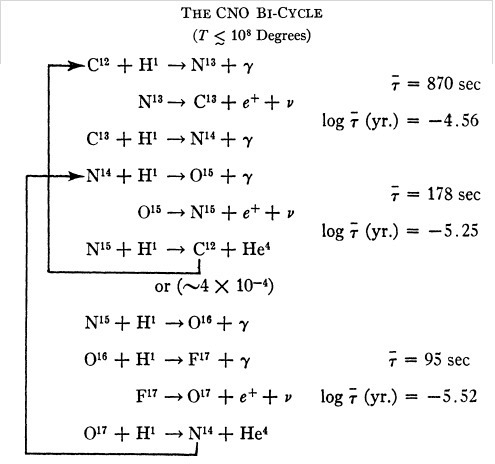
\includegraphics[width=(\textwidth),height=(\textheight-11mm),keepaspectratio]{cnobi}
\caption{Bi-ciclo CNO.}
\end{figure}

\begin{align*}
^{12}_6C+^1H\to^{13}_7N+\gamma\\
^{13}N\to ^{13}_6C+\APelectron+\Pnu\\
^{13}C+^1H\to ^{14}_7N+\gamma\\
^{14}_7N+^1H\to ^{15}_8O+\gamma\\
^{15}_8O\to ^{15}_7N+\APelectron+\gamma\\
^{15}_7N+^1H\to ^{12}_6C+^4_2He
\end{align*}

Processo efficace:

$4^1H\to ^4He+2\APelectron+2\Pnue$ uguale alla catena PP, stesso Q-valore.

\clearpage



\chapter{Strutture degeneri}
\PartialToc

\section{Degenerazione}

Il sole \'e descrivibile con equazioni non degeneri le nane bianche con equazioni degeneri.

\subsection{Electron's degeneracy}
The degeneracy is due to Pauli exclusion principle for electron rather than gas density approaching nuclear densities: $\rho_N\approx10^{12}g/cm^3$ which is more than a factor $10^3$ higher than the highest densities we will encounter.

\begin{equation*}
n_E\,d^3p_e\,d^3x\leq\frac{2}{h^3}\,d^3p_e\,dV
\end{equation*}

If we put more electrons in our small space volume the maximum of distribution function will soon approach the ceiling.

\subsection{Complete degeneracy}

Derivo l'equazione di stato per un gas completamente degenere: determino pressione e densit\'a.

Relazione tra impulso di Fermi e densit\'a.

\begin{align*}
&N_E=\frac{1}{V}\int_{|p|=0}^{|p|=p_0}\frac{2}{h^3}\,d^3p\,d^3x=\frac{2}{h^3}\frac{4\pi}{3}p_0^3\\
&N_E=\frac{1}{\mu_E}\frac{\rho}{m_p},\quad\frac{1}{\mu_E}=X+\frac{1}{2}Y+\frac{1}{2}Z\\
&=\frac{1}{2}(1+X)&\intertext{Risolvendo le ultime 2 equazioni ricavo la densit\'a in funzione dell'impulso di Fermi}\\
&\frac{1}{\mu_E}\rho=\frac{8\pi}{3}\frac{m_P}{h^3}p_0^3\\
\end{align*}

Relazione tra impulso di Fermi e pressione.

\begin{align*}
&P_E=\int_{|p|=0}^{|p|=p_0}p_xv_x\frac{2}{h^3}\,d^3p&\intertext{$\uparrow$ is rate of transport of momentum: the momentum $p_x$ of a cubic centimeter transported through a square centimeter at rate given by $v_x$. That here we have singled out the x direction is of no consequence since the momentum distribution is spherical.}\\
&P_E=\frac{8\pi}{15mh^3}p_0^5&\intertext{$\uparrow$ espressione per velocit\'a non relativistiche: ho usato $v_x=\frac{p_x}{m}$.}\\
&P_E=\frac{2\pi c}{3h^3}p_0^4&\intertext{$\uparrow$ espressione per velocit\'a relativistiche: ho usato $v_x=c\frac{p_x}{|p|}$.}
\end{align*}

Equazione di stato.
\begin{align*}
&P_E=K_{NR}(\frac{1}{\mu_E}\rho)^{\frac{5}{3}}&\intertext{$\uparrow$ equazione di stato per gas di elettroni completamente degenere non relativistico, }\\
&K_{NR}=\frac{h^2}{20m_em_p}(\frac{3}{\pi m_p})^{\frac{2}{3}}=9.91*10^{12}\\
&P_E=K_R(\frac{1}{\mu_E}\rho)^{\frac{4}{3}}&\intertext{$\uparrow$ equazione di stato per gas di elettroni completamente degenere relativistico, }\\
&K_R=\frac{hc}{8m_p}(\frac{3}{\pi m_p})^{\frac{1}{3}}=1.23*10^{15}
\end{align*}

La pressione totale \'e $P=P_A+P_E$ dove $P_A$ \'e data dall'equazione dei gas perfetti: all'equilibrio termico gli atomi hanno la stessa energia per particella degli elettroni quindi data la maggiore massa hanno un momento maggiore di $\sqrt{\frac{m_A}{m_E}}$ e occupano un volume nello spazio dell fasi $(\frac{m_A}{m_E})^{\frac{3}{2}}$ maggiore degli elettroni: gli atomi hanno a disposizione un volume dello spazio delle fasi $10^5$ volte maggiore degli elettroni.

\section{Region in diagram density-temperature and equation of state}

\begin{figure}[!ht]
\centering
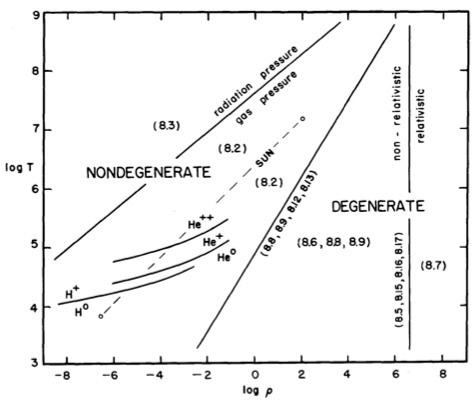
\includegraphics[width=(\textwidth),height=(\textheight-11mm),keepaspectratio]{Trho-state}
\caption{Equazione di stato nel diagramma densit\'a-Temperatura.}
\end{figure}

\subsection{Degeneracy limits}
Cerco il confine nel diagramma temperatura-densit\'a fra regione degenere e non-degenere e, nella regione degenere tra la parte relativistica e non relativistica.

Definisco il limite tra le regione degenere/non-degenere attraverso l'uguaglianza
\begin{align*}
\frac{1}{\mu_E}\frac{K}{m_P}\rho T=K_{NR}(\frac{1}{\mu_E}\rho)^{\frac{5}{3}}&\intertext{Risolvendo $\uparrow$ per la densit\'a:}\\
\frac{1}{\mu_E}\rho=(\frac{KT}{m_PK_{NR}})^{\frac{3}{2}}=2.4*10^{-8}T^{\frac{3}{2}}
\end{align*}

e il confine tra regione non-relativistica e relativiastica uguagliando la pressione data delle risp. formule
\begin{equation*}
\frac{1}{\mu_E}\rho=(\frac{K_R}{K_{NR}})^3=1.916*10^6
\end{equation*}

\subsection{Radiation/gas pressure limit}

The upper left corner represent the region where radiation pressure is dominant. The boundary line represents the equation \mblock{P_{Rad}=P_G}.

Throughout the majority of stars radiation pressure is of no importance.


\section{Electron degeneracy}

\subsection{Boltzmann statistic}

High density in volume $dV$ so that is fully pressure ionized: free electron of density $n_e$. If the velocity distro is given by Boltzmann statistic their mean kinetic energy is \mblock{\frac{3kT}{2}}: the number of electrons in spherical shell $[p,p+dp]$ is
\begin{equation*}
f(p)\,dp\,dV=n_e\frac{4\pi p^2}{(2\pi m_ekT)\expy{\frac{3}{2}}}\exp{-\frac{p^2}{2m_ekT}}\,dp\,dV
\end{equation*}

A reduction of $T$ with $n_e$ constant cause maximum of distro function $p_{max}=\sqrt{2m_ekT}$ to tends to smaller values of $p$ and the maximum of $f(p)$ becomes higher since \mblock{n_e=\intzi f(p)\,dp}

\subsection{Pauli principle}

Each quantum cell of 6D phase space can't contain more than 2 electrons with \mblock{d^3pdV=h^3}: in the shell \mblock{[p,p+dp]} of momentum space there are \mblock{4\pi p^2\,dp\,dV/h^3} quantum cells which can't contain more than \mblock{2*4\pi p^2\,dp\,dV/h^3}:
\begin{equation*}
f(p)\,dp\,dV\leq2*4\pi p^2\,dp\,dV/h^3
\end{equation*}

The Boltzmann distro for $n_e$ constant is in contraddiction with QM for low T.

\subsection{Complete degeneracy: T=0.}

The state in which all electrons have lowest energy without violating PP is that in which all phase cells are occupied up to $p_F$
\begin{align*}
&f(p)=\frac{8\pi p^2}{h^3}\ p\leq p_F\\
&f(p)=0\ p\geq p_F
\end{align*}

quindi
\begin{align*}
&n_e\,dV=dV\int_0^{p_F}\frac{8\pi p^2\,dp}{h^3}=\frac{8\pi}{3h^3}p_F^3\,dV:\\
&p_F\propto n_e\expy{\frac{1}{3}}&\intertext{non relativistic:}\\
&E_F=\frac{p_F^2}{2m_e}\propto n_e\expy{\frac{2}{3}}
\end{align*}

If density is high enough we can have velocity comparable to $c$:

\begin{align*}
&p=\frac{m_ev}{\sqrt{1-v^2/c^2}}\\
&E_{tot}=\frac{m_ec^2}{\sqrt{1-v^2/c^2}}=m_ec^2\sqrt{1+\frac{p^2}{m_e^2c^2}}
\end{align*}

Kinetic energy \mblock{E=E_{tot}-m_ec^2}

\begin{definition}{Peso molecolare medio per elettrone libero}
Mette in relazione la densit\'a col numero di elettroni liberi:
numero di \Pelectron per $cm^3$ \'e la densit\'a ($\rho$) moltiplicato moli di lettroni libero per grammo ($\frac{1}{\mu_e}$) moltiplicato $N_A\approx\frac{1}{m_p}$.
\end{definition}

\begin{usefull}{Pressure completely deg electron gas}
The pressure is the flux of momentum per unit surface per unit time: each electrons carries momentum p in direction $\hat{s}$, the component in direction $\hat{n}$ is \mblock{p\cos{\theta}}

At location of surface element there are \mblock{f(p)\,dp\,d\Omega_s/(4\pi)} electrons per unit volume with right momentum (right p and right direction): the flux of particles with \mblock{p\in[p,p+dp]} and direction within $d\Omega_s$ is  \mblock{f(p)\,dp\,d\Omega_sv(p)\cos{\theta}\,d\sigma/(4\pi)}. $\cos{\theta}$ arises since electrons moving into solid angle see only a projection of $d\sigma$.

Non relativistic pressure:
consiriomo gli \Pelectron completamente degeneri quindi lo le celle dello spazio delle fasi sono accupate con 2 elettroni fino a $p_F$ (densit\'a di stati: \mblock{\phi_e\,d^3x\,d^3p=\frac{2}{h^3}\,d^3x\,d^3p})
\mblock{P_e=\frac{8\pi}{3h^3}\int_0^{p_F}p^3v(p)\,dp}.

Relativistic:

\begin{align*}
&P_e=\frac{\pi m_e^4c^5}{3h^3}f(x)=\frac{8\pi c^5m_e^4}{3h^3}\int_0^x\frac{\xi^4\,d\xi}{\sqrt{1+\xi^2}}\\
&\xi=\frac{p}{m_ec},\ x=\frac{p_F}{m_ec}\\
&n_e=\frac{\rho}{\mu_em_u}=\frac{8\pi m_e^3c^3}{3h^3}x^3
\end{align*}


\end{usefull}

Internal energy of electron gas per unit volume:

\begin{align*}
&u_e=\int_0^{p_F}f(p)E(p)\,dp=\frac{8\pi}{h^3}\int_0^{p_F}E(p)p^2\,dp\\
&u_e=\frac{\pi m_e^4c^5}{3h^3}g(x)
\end{align*}

\subsection{Importance of relativistic effects: limiting case.}

The param \mblock{x\ (x_F=\frac{p_F}{m_ec})} is a measure of importance of relativistic effects.

\begin{usefull}{Electron degeneracy: non-relativistic limit pressure}
\begin{align*}
&x=\frac{p_F}{m_ec}=\frac{v_F/c}{\sqrt{1-v_F^2/c^2}}:\ \frac{v_F^2}{c^2}=\frac{x^2}{1+x^2}\\
&x\to0: f(x)\to\frac{8}{5}x^5,\ g(x)\to\frac{12}{5}x^5&\intertext{$x\ll1$: relativistic effects can be ignored:}\\
&P_e=\frac{1}{20}(\frac{3}{\pi})\expy{\frac{2}{3}}\frac{h^2}{m_e}n_e\expy{\frac{5}{3}}\\
&=\frac{1}{20}(\frac{3}{\pi})\expy{\frac{2}{3}}\frac{h^2}{m_em_u\expy{\frac{5}{3}}}(\frac{\rho}{\mu_e})\expy{\frac{5}{3}}\\
&=\num{1.0036e13}(\frac{\rho}{\mu_e})\expy{\frac{5}{3}}\ (cgs)\\
&P_e=\frac{2}{3}U_e
\end{align*}
\end{usefull}

\begin{usefull}{Electron degeneracy: relativistic limit pressure}
\begin{align*}
&x\to\infty: f(x)\to2x^4,\ g(x)\to6x^4&\intertext{for extreme relativistic case $x\gg1$:}\\
&P_e=(\frac{3}{\pi})\expy{\frac{1}{3}}\frac{hc}{8}n_e\expy{\frac{4}{3}}\\
&=\num{1.2435e15}(\frac{\rho}{\mu_e})\expy{\frac{4}{3}}\ (cgs)\\
&P_e=\frac{1}{3}U_e
\end{align*}
\end{usefull}

\subsection{Relazione densit\'a energia cinetica-Pressione}

Ricavo la relazione densit\'a di energia cinetica-pressione.

\begin{align*}
\epsilon=\frac{E}{V}=\frac{1}{V}\frac{3}{2}NK_BT&\intertext{Relazione tra pressione e concentrazione degli elettroni.}\\
P=\frac{2}{3}\epsilon
\end{align*}


\subsection{Degenerazione parziale}

The most probable occupation of phase cells of shell $[p,p+\,dp]$ in momentum space is determined by FD statistic
\begin{align*}
f(p)\,dp\,dV=\frac{8\pi p^2\,dp\,dV}{h^3}*\frac{1}{1+\exp{\frac{E}{KT}-\psi}}&\intertext{$\Psi$ \'e il parametro di degenerazione}
\end{align*}

\subsection{Gas di Fermi non relativistico}

\begin{itemize*}

\item Degenerazione.

\begin{equation*}
n_e\,d^3x\,d^3p\leq2\frac{d^3x\,d^3p}{h^3}
\end{equation*}

\item Densit\'a di stati.


\begin{align*}
&dN=\frac{1}{8}4\pi n^2dn&\intertext{da cui ricavo la densit\'a imponendo le condizioni periodiche al bordo del volume $V=L^3$}\\
&g(k)=\frac{dN(k)}{d^3k}=\frac{dN(k)}{4\pi k^2dk}=\frac{\nu V}{(2\pi)^3}
\end{align*}

\item Energia gas di Fermi completamente degenere: $T=0$.
\begin{align*}
&N=\int g(k)F(k)d^3k=\frac{\nu V}{(2\pi)^3}\int_0^{K_F}4\pi k^2\,dk\\
&=\frac{\nu V}{2\pi^2}\frac{k_F^3}{3}
\end{align*}
da cui ricavo la densit\'a
\begin{equation*}
n=\frac{\nu}{6\pi^2}k_F^3
\end{equation*}
e adesso introduco la densit\'a di energia e ricavo la sua dipendenza da n
\begin{align*}
&\epsilon=\frac{\hbar^2k^2}{2m_0}\quad(\epsilon_F=\frac{\hbar^2k_F^2}{2m_0})\\
&E=\int\epsilon(k)F(k)g(k)d^3k=\frac{\nu V}{2\pi^2}\frac{\hbar^2}{2m_0}\frac{k_F^5}{5}\\
&\frac{E}{N}=\frac{3}{5}\epsilon_F\\
&\epsilon=\frac{E}{V}=\frac{E}{N}\frac{N}{V}=\frac{3}{5}\epsilon_Fn\propto n^{\frac{5}{3}}
\end{align*}

\item Pressione di un gas di Fermi di elettroni completamente degenere
\begin{align*}
&P=-\frac{\partial E}{\partial V}|_{S,N}=n^2\frac{\partial(\frac{E}{N})}{\partial n}|_{S,N}\propto n^{\frac{5}{3}}\\
&P=K_{NR}\rho^{\frac{5}{3}}\\
&P=\frac{1}{20}(\frac{3}{\pi})^{\frac{2}{3}}\frac{h^2}{m_e}n_e^{\frac{5}{3}}=\frac{1}{20}(\frac{3}{\pi})^{\frac{2}{3}}\frac{h^2}{m_em_u^{\frac{5}{3}}}(\frac{\rho}{\mu_e})^{\frac{5}{3}}\\
&=1.0036*10^{13}(\frac{\rho}{\mu_e})^{\frac{5}{3}}\quad(cgs)\\
&P=\frac{2}{3}U_e
\end{align*}

\end{itemize*}

\subsection{Gas di Fermi relativistico}

\begin{itemize*}

\item Energia.

\begin{equation*}
\epsilon(k)=\sqrt{(\hbar ck)^2+(m_0c^2)^2}
\end{equation*}

\item Parametri adimensionali.

\begin{align*}
y=\frac{\hbar}{m_0c}k=\lambdabar k\\
\lambdabar k_F=x
\end{align*}

\item densit\'a di particelle.

\begin{equation*}
n=\frac{8\pi c^3m^3}{3h^3}x^3=5.87*10^{29}x^3
\end{equation*}

\item Pressione.

\begin{align*}
&P\propto n^{\frac{4}{3}}\\
&P=(\frac{3}{\pi})^{\frac{1}{3}}\frac{hc}{8}n_e^{\frac{4}{3}}=(\frac{3}{\pi})^{\frac{2}{3}}\frac{hc}{8m_u^{\frac{4}{3}}}(\frac{\rho}{\mu_e})^{\frac{4}{3}}\\
&=1.2435*10^{15}(\frac{\rho}{\mu_e})^{\frac{4}{3}}\quad(cgs)\\
&P=\frac{1}{3}U_e
\end{align*}

\end{itemize*}

\subsection{Relazione densit\'a-pressione(-impulso di Fermi) per gas degenere}

Per un gas completamente degenere di elettroni
\begin{align*}
&E_F\propto n_e^{\frac{2}{3}}&\intertext{$\uparrow$ Non-relativistico}\\
&E_F\propto n_e^{\frac{1}{3}}&\intertext{$\uparrow$ Ultra-Relativistico}
&P\propto n_e^{\frac{5}{3}}&\intertext{$\uparrow$ Non-relativistico}\\
&P\propto n_e^{\frac{4}{3}}&\intertext{$\uparrow$ Ultra-Relativistico}
\end{align*}
\index{Rivedere relazione energia fermi densita elettroni}


\subsection{Partial degeneracy}

For finite T not all electrons will be packed in momentum space in lowest possible momentum: if T is high enough we expect them to have a Boltzmann distro.

The most probable occupation of the phase cells of shell \mblock{[p,p+dp]} is determined by FD statistic
\begin{equation*}
f(p)\,dp\,dV=\frac{8\pi p^2\,dp\,dV}{h^3}=\frac{1}{1+\exp{\frac{E}{kT}-\psi}}
\end{equation*}
if $p\leq p_F$ there are fewer electrons than for $T=0$.

For non-relativistic case: $E=\frac{p^2}{2m_e}$
\begin{align*}
&n_e=\frac{8\pi}{h^3}\intzi{}\frac{p^2\,dp}{1+\exp{\frac{p^2}{2m_ekT}-\psi}}\\
&=\frac{8\pi}{h^3}(2m_ekT)\expy{\frac{3}{2}}a(\psi)\\
&a(\psi)=\intzi{}\frac{\eta^2}{1+\exp{(\eta^2-\psi)}}
\end{align*}

The degeneracy parameter is a function of \mblock{\psi(\frac{n_e}{T\expy{\frac{3}{2}}})}.

For large negative value of $\psi$, $a(\psi)$ can be made arbitrarily small: for a given electron density this is the case for high T: $f(p)$ must become Boltzmann distro and (\mblock{\frac{E}{kT}=\frac{p^2}{2m_ekT}}) \mblock{\exp{\psi}=\frac{h^3n_e}{2(2\pi m_ekT)\expy{\frac{3}{2}}}}

\section{White dwarfs}

\subsection{Grandezze caratteristiche}

\begin{itemize*}
\item $M\approx\msun$
\item $\rho_c\approx10^6gr/cm^3\approx10^4\rhosunc$.
\begin{align*}
&n_e=\exv{Z}n_I\\
&\rho=\exv{m_I}n_I+m_en_e\\
&\approx\exv{M_{atom}}n_I=\exv{A}m_Hn_I
\end{align*}

\item Raggio di Schwarzschild.

\begin{equation*}
\frac{R_G}{R}\approx100(\frac{R_G}{R})_{\odot}\approx4*10^{-6}
\end{equation*}
ho definito il raggio di Schwarzchild come $R_G=\frac{2GM}{c^2}$.
\item Velocit\'a di fuga.

\begin{equation*}
v_f=\sqrt{\frac{2GM}{R}}\approx0.02 c
\end{equation*}

\item Pressione.

\begin{equation*}
P=P_I+P_{el}\approx P_{el}
\end{equation*}
\end{itemize*}

\subsection{Application of complete degenerate statistic}

\begin{align*}
&T=0\\
&3(\gamma-1)U=-\Omega=\frac{3}{5}\frac{GM^2}{R}\\
&U=VE_e,\ E_e=12A\frac{x^5}{5}\\
&x_F=\frac{p_F}{mc},\ x(\frac{\rho}{\mu_e}),\ \rho\propto\frac{M}{R^3}\\
&n_e=\frac{8\pi}{3}(\frac{h}{m_ec})\expy{-3}x^3=\num{5.865e29}x_F^3\si{\per\cubic\cm}
\end{align*}

\begin{usefull}{WD: Non relativistic mass-radius relation}
Per densit\'a costante

\begin{align*}
&M\propto(\frac{h^2N_A}{m_eG})^3\frac{N_A^2}{\mu_e^5}\frac{1}{R^3}\\
&\frac{M}{\msun{}}\approx\num{e-6}(\frac{R}{\rsun{}})\expy{-3}(\frac{2}{\mu_e})^5
\end{align*}
Fatti:
\begin{itemize}
    \item Abbiamo assunto $P_e$, $E_e$ costanti: la maniera corretta \'e usare l'espressione generale per la pressione (\mblock{v=\PDy{p}{E_k}})
\end{itemize}
\end{usefull}



\begin{usefull}{\cha{} limiting mass}
In the limit of extreme relativistic degeneracy
\begin{equation*}
\frac{M}{\msun{}}=\frac{M_{ch}}{\msun{}}=1.456(\frac{2}{\mu_e})^2
\end{equation*}
\end{usefull}

\subsection{How far inward before degeneracy set in?}

Condizione necsuff perch\'e si abbia degenerazione \'e
\begin{align*}
\frac{4\pi^2}{(\theta mc^2)^2}\frac{x\sqrt{x^2+1}}{f(x)}\gg1&\intertext{ho definito}\\
x=\frac{h}{mc}(\frac{3n}{8\pi})^{\frac{1}{3}}\quad \theta=\frac{1}{KT}
\end{align*}
Per gli strati esterni vale $P\propto\rho T$ ($\approx0.23 \%$ della massa) 



\subsection{Equazione di stato degli Ioni}
\begin{equation*}
N_E=\frac{1}{\mu_E}\frac{\rho}{m_P}\quad\frac{1}{\mu_E}=X+\frac{1}{2}Y+\frac{1}{2}Z\approx\frac{1}{2}(1+X)
\end{equation*}

Condizioni per la degenerazione degli atomi: nuclei have on the average the same energy as electron, il momento \'e maggiore di un fattore radice quadrata del rapporto fra le masse per grado di libert\'a e quindi sono distribuiti nello spazio delle fasi su un volume $(2000)^{\frac{3}{2}}$ maggiore.
Per gli atomi possiamo usare
\begin{equation*}
P_A=\frac{1}{\mu_A}\frac{K}{m_P}\rho T\quad\frac{1}{\mu_A}=X+\frac{1}{4}Y
\end{equation*}

\subsection{Interazione Ioni-elettroni}
Il contributo Coulombiano alla pressione diminuisce la massa limite:
\begin{equation*}
P_C\propto-e^2\exv{Z}^{\frac{2}{3}}n_e^{\frac{4}{3}}<0
\end{equation*}

\subsection{Boundaries between D/ND and in latter R/NR}

Electron pressure for complete degeneracy
\begin{equation*}
P_E=\int_{|p|\leq p_0}\,d^3p\,p_xv_x\frac{2}{h^3}
\end{equation*}
e utilizzando l'opportuna relazione (R/NR) tra v e p trove la pressione nei due casi per gas di elettroni completamente degenere

\begin{itemize*}
\item Relativistico: $v=\frac{p}{m}$.
\begin{equation*}
P_E=\frac{2\pi c}{3h^3}p_0^4=K_2(\frac{\rho}{\mu_E})^{\frac{4}{3}}
\end{equation*}

\item Non relativistico $v_x=c\frac{p_x}{|p|}$.
\begin{equation*}
P_E=\frac{8\pi}{15mh^3}p_0^5=K_1(\frac{\rho}{\mu_E})^{\frac{5}{3}}
\end{equation*}

\end{itemize*}

\begin{itemize*}
\item Confine tra zona degenere e non degenere.

\begin{align*}
&\frac{1}{\mu_E}\frac{K}{m_P}\rho T=K_1(\frac{\rho}{\mu_E})^{\frac{5}{3}}\\
&\frac{1}{\mu_E}\rho=(\frac{KT}{m_PK_1})^{\frac{3}{2}}
\end{align*}

\item Confine tra zona degenere relativistica e non.

\begin{equation*}
\frac{1}{\mu_E}\rho=(\frac{K_2}{K_1})^3=1.916*10^6
\end{equation*}

\end{itemize*}

\subsection{Mass/radius relation}

L'equazioni di stato \'e indipendente da T
\begin{align*}
P=\frac{\pi m^4c^5}{3h^3}f(x)\\
\rho=\mu_E\frac{8\pi m_Pm^3c^3}{3h^3}x^3&\intertext{con}\\
x=\frac{p_0}{mc}\quad \mu_E=\frac{2}{1+X}
\end{align*}
Posso separare il problema idrostatico da quello termodinamico.

Equilibrio idrostatico:
\begin{align*}
\frac{dP}{dr}=-\rho\frac{GM_r}{r^2}\\
\frac{dM_r}{dr}=4\pi r^2\rho
\end{align*}
da integrare numericamente(Chandrasekhar).

Qualitativamente
\begin{itemize*}
\item The larger the mass of a white dwarf the smaller the radius.
\item Per nane bianche con circa massa solare il raggio \'e centinaia di volte pi\'u piccolo del sole.
\end{itemize*}

\begin{figure}[!ht]
\centering
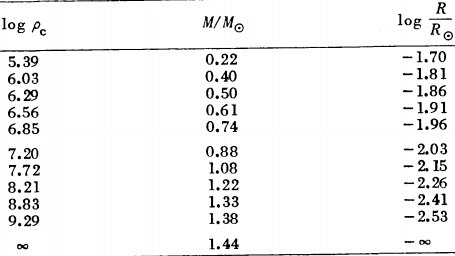
\includegraphics[width=(\textwidth),height=(\textheight-11mm),keepaspectratio]{MRWD}
\caption{Mass/radius relation for completely degenerate WD.}
\end{figure}

\subsection{Limite superiore per la massa di una stella completamente degenere}

Quantit\'a che influenzano l'equilibrio idrostatico:
\begin{align*}
\rho\propto\frac{M}{R^3}&\intertext{questa sopra \'e la densit\'a, questa sotto l'attrazione gravitazionale}\\
\rho\frac{GM_r}{r^2}\propto\frac{M^2}{R^5}
\end{align*}

Per la pressione:
\begin{align*}
P\propto\rho^{\frac{5}{3}}\propto\frac{M^{\frac{5}{3}}}{R^5}&\intertext{per stelle meno massive ho la pressione NR (sopra), per stelle massive uso la formula R (sotto)}\\
P\propto\rho^{\frac{4}{3}}\propto\frac{M^{\frac{4}{3}}}{R^4}
\end{align*}

il cui gradiente genera una forza di pressione
\begin{align*}
F_P&\propto\frac{M^{\frac{5}{3}}}{R^6}\quad\text{NR-D}\\
&\frac{M^{\frac{4}{3}}}{R^5}\quad\text{R-D}
\end{align*}

Osservazioni:
\begin{itemize*}
\item In the relativistic case gravitational force and pressure force depend on the same power of radius.
\item In R-D the 2 forces depend on different power of mass.
\end{itemize*}

\subsection{Massa di Chandrasekhar}

La densit\'a centrale di una nana bianca aumenta come $M^2$ fino all'istaurarsi del regime ultra-relativistico: in regime UR solo una massa \'e in equilibrio.

Usando un modello politropico ricavo
\begin{align*}
M_{Ch}=(\frac{2}{\mu_e})^2*1.459\msun&\intertext{Per nane bianche di He o C ho $\downarrow$}\\
M_{Ch}=1.4\msun
\end{align*}

Per una stella omogenea il T. del viriale ci dice
\begin{align*}
2\int\epsilon_{Cin}\,dV=\frac{3}{5}\frac{GM^2}{R}=\frac{3}{5}G(\frac{4\pi}{3})^{\frac{1}{3}}M^{\frac{5}{3}}\rho^{\frac{1}{3}}
\end{align*}

Nel caso non relativistico

\begin{align*}
&\frac{3}{5}G(3\pi^2)^{\frac{2}{3}}\frac{\hbar^2}{m_e}(\frac{1}{\mu_em_P})^{\frac{5}{3}}M\rho^{\frac{2}{3}}&\intertext{$\mu_e$ \'e il peso molecolare medio quando si considera il contributo alla pressione del gas solo degli elettroni: $\mu_e=1$ per $^1H$, $\mu_e\approx2$ per altri casi($\geq2$ adroni per elettrone). Ho usato $\downarrow$}\\
&P=\frac{1}{20}(\frac{3}{\pi})^{\frac{2}{3}}\frac{h^2}{m_e}n_e^{\frac{5}{3}}=\frac{1}{20}(\frac{3}{\pi})^{\frac{2}{3}}\frac{h^2}{m_em_u^{\frac{5}{3}}}(\frac{\rho}{\mu_e})^{\frac{5}{3}}\\
&=1.0036*10^{13}(\frac{\rho}{\mu_e})^{\frac{5}{3}}\quad(cgs)\\
&P=\frac{2}{3}U_e
\end{align*}

\begin{align*}
\rho\propto G^3(\mu_em_P)^5m_e^3M^2
\end{align*}

Nel caso relativistico

\begin{align*}
M\propto(\frac{c\hbar}{G})^{\frac{3}{2}}\frac{1}{\mu_e^2m_P^2}\to M_{Ch}
\end{align*}

\subsection{WD oscillations.}

Prendendo $\Delta R\approx1\%$:
\begin{equation*}
\Delta E_{grav}\propto \frac{GM^2}{R}\frac{\Delta R}{R}\approx\SI{e48}{\erg}
\end{equation*}

\section{Stelle di neutroni}

\subsection{Formazione}

Nascono dal collasso di una stella ed hanno $T\geq10^{10}\,K$: rapidamente la temperatura della stella diminuisce a causa del flusso di neutrini. In 100 yr $T\approx10^8$, che pu\'o essere considerata bassa vista l'energia massima dei neutroni altamente degeneri:
\begin{align*}
KT\approx10\,KeV\\
E_F\approx1000\,MeV
\end{align*}
L'equazione di stato \'e essenzialmente la stessa che per $T\approx0$.

\subsection{Neutronizzazione}

L'aumento della densit\'a aumenta l'energia degli elettroni che danno luogo con i protoni a electron capture. I nuclei arricchiti di neutroni ($^{118}Kr$) cominciano ad emetterli a una densit\'a $\rho_{dr}\approx4*10^{11}g/cm^3$.\index{Neutron drip}

In questo stadio la materia \'e composta da nuclei (di solito organizzati in reticolo), elettroni e neutroni liberi: il numero di elettroni aumenta con la densit\'a e cos\'i $P_n$.

\begin{align*}
P\approx P_e\gg P_n&\intertext{$\uparrow$ per $\rho\approx\rho_{dr}$}\\
p_n\approx\frac{P}{2}&\intertext{$\uparrow$ per $\rho\approx10^{12}gr/cm^3$}
\end{align*}

\subsection{Fasi successive: Hyperionizzation.}

A partire dall densit\'a per cui i nuclei sono in contatto $\rho_{Nuc}\approx2.4*10^{14}gr/cm^3$ ho un gas/liquido di neutroni degeneri in equilibrio con piccola frazione di \Pproton, \Pelectron: $\Pneutron\leftrightarrow\Pproton+\Pelectron$. 

Successivamente ho iperionizzazione e quark liberi.

\subsection{Massa limite per stelle di neutroni}

Uso i conti fatti per le nane bianche con opportuno scaling

\begin{align*}
m_e\to m_n\\
\underbrace{\mu_{WD}}_2\to\underbrace{\mu_{NS}}_1\\
\end{align*}

ottengo

\begin{align*}
&\rho^{NS}(M)=\rho^{WD}(M)(\frac{m_n}{m_e})^3(\frac{\mu_{NS}}{\mu_{WD}})^5\\
&\approx2.5*10^8\rho^{WD}(M)\\
&\rho^{NS}(M)\approx2.5*10^{14}(\frac{M}{\msun})^2g/cm^3
\end{align*}

e per la massa limite di una stella di neutroni ottengo
\begin{equation*}
M_{Cha}^{NS}=M_{Cha}(\frac{\mu_{WD}}{\mu_{NS}})^2\approx5.7\msun
\end{equation*}
Calcoli pi\'u precisi abbassano il limite?

\section{Buchi neri}

\subsection{Raggio di Schwarzschild}

Alla superficie di una configurazione di massa M e raggio R la curvatura gaussiana dello spazio \'e 
\begin{align*}
&K_G=\frac{GM}{c^2R^3}=-\frac{1}{2}\frac{r_s}{R}\frac{1}{R^2}&\intertext{\'e solitamente piccolo rispetto alla curvatura $R^{-2}$ della superficie sferica:}\\
&-K\approx2*10^{-6}\frac{1}{R^2}&\intertext{$\uparrow$ at surface of the sun}\\
&-K\approx0.15\frac{1}{R^2}&\intertext{$\uparrow$ for neutron star}\\
&-K\approx\frac{1}{R^2}&\intertext{$\uparrow$ for black hole with $R=r_s$}
\end{align*}

Il parametro critico \'e il raggio di Schwarzschild
\begin{equation*}
r_s=\frac{2MG}{c^2}
\end{equation*}
cio\'e la distanza dal centro di attrazione di una massa per cui $v_f=c$.

\subsection{Densit\'a critica}

In termini di densit\'a ho
\begin{align*}
\rho_{Crit}\approx2*10^{16}(\frac{\msun}{M})^2g/cm^3
\end{align*}

\part{Modello ed evoluzione stellare.}

\documentclass[main.tex]{subfiles}

\begin{document}
\chapter{Formation of a star from interstellar medium}
\PartialToc

\section{Broader problem of formation of a star}
(Burbidge (1960), Kahn (1960), Ebert-von Hoerner-Temesvary (1960))

Change in density from \SIrange{e-24}{1}{\gram\per\cubic\cm}

\section{Final stage of formation}
A star without neclear reactions:
\begin{itemize}
\item Optically thick system: radiation escapes only from thin surface layer
\item Hydrodynamic time-scale must be much shorter than thermal time-scale: we can calculate heat flow assuming HE.
\end{itemize}
 
\subsection{Conditions for homologous contraction}

$\TDly{\rho}{T}$: in a log-plot of temperature vs density profile during contraction every point evolve parallel to the $p_g=P_r$ line.

\chapter{Fonti energia: energia gravitazionale ed energia interna.}

A star derives its energy to shine from internal energy, thermonuclear fuel, and gravitational contraction.
\PartialToc


\section{Equilibrio meccanico locale vs constrain on star's structure}

\subsection{G-nal potential energy}
(vedi ~\ref{chap:gravity}) L'energia potentziale gravitazionale di un corpo autogravitante \'e l'opposto dell'energia necessaria per portare le masse infinitesime arbitrariamente lontane:
\begin{align*}
&d\Omega=-\int_r^{\infty}\frac{Gm(r)}{r'^2}\,dm(r)\,dr'\\
&=-\frac{Gm(r)}{r}\,dm(r)\\
&\Omega=-\int_0^M\frac{Gm(r)}{r}\,dm(r)\\
&\Omega=-q\frac{GM^2}{R}&\intertext{per densit\'a uniforme}\\
&\Omega=-\frac{3}{5}\frac{GM^2}{R}
\end{align*}

\subsection{\kh{} time-scale (sole)}
Nel caso del sole: divido l'energia potentziale G-nal per la luminosit\'a attuale
\begin{equation*}
\frac{G\msun}{\rsun}\approx\num{3.8e48}\si{\erg}/\lsun\approx\num{3e7}\,yr
\end{equation*}

\subsection{Mechanical and internal energy}

Trascuro i moti macroscopici o fenomeni turbolenti: l'energia totale di una stella

\begin{align*}
&W=\int_ME\,dm(r)+\Omega=U+\Omega\\
&U=\int_ME\,dm(r)
\end{align*}

\subsection{Equilibrium state. Adiabatic perturbation.}

Equilibrium state of the star corrisponds to extrema of $W$: hydrostatic equilibrium is an extremum relative to other configurations.

For adiabatic perturbation (abbastanza rapide da pater trascurare gli scambi di calore e abbastanza lente da poterne trascurare l'energia cinetica, adiabatic sound waves) 

\begin{align*}
&\varad{W}=0&\intertext{$\uparrow$ hydrostatic stellar equilibrium}\\
&\varad{W}=\varad{U}+\varad{\Omega}\\
&U\to U+\varad{U}=U+\delta\int_ME\,dm(r)\\
&=U+\int\delta E\,dm(r)&\intu{changes in specific internal energy of a particular mass element $dm(r)$ (Lagrangian description of the perturbation).}
\end{align*}

We label each mass element of $dm(r)$ worth of matterand see what happens to $E$ when $r$, $T$ and $\rho$ change.

\begin{align*}
&dQ=dE+P\,d\vrho{}=T\,dS&\intu{1 e 2 leggi termodinamica}\\
&\vrho=\frac{1}{\rho}
\end{align*}
Qui scrivo $\vrho{}$ per indicare il volume specifico con dimensioni \si{\cubic\cm\per\gram} cio\'e il volume associato ad 1 grammo di materia:
\begin{align*}
&\vrho{}=\frac{1}{\rho}=\frac{4\pi r^2\,dr}{dm(r)}=\frac{d(\frac{4\pi r^3}{3})}{dm(r)}\\
&\vrho{}\to\vrho{}+\var{\vrho{}}=\frac{d[4\pi\frac{(r+\var{r})^3}{3}]}{dm(r)}\vrho{}\\
&+\frac{d(4\pi r^2\var{r})}{dm(r)}&\intu{al primo ordine in $\var{r}$: $\frac{\var{r}}{r}\ll1$ and ''spherically symmetric'' perturbation.}
\end{align*}

\begin{align*}
&\varad{U}=-\int_MP\var{\vrho{}}\,dm(r)\\
&=-\int_MP\TDof{m_r}(4\pi r^2)\,dm_r\\
&\varad{U}=\int_M\TDy{m_r}{P}4\pi r^2\var{r}\,dm_r&\intu{Boundary conditions:}\\
&\var{r}(m_r=0)=0,\quad P_S=P(m_r=M)=0\\
\end{align*}

Per l'energia potenziale gravitazionale
\begin{align*}
&\Omega\to\Omega+\var{\Omega}=-\int_M\frac{Gm_r}{r+\var{r}}\,dm_r=\\
&\approx\Omega+\int_M\frac{Gm_r}{r^2}\var{r}\,dm_r
\end{align*}

\begin{align*}
&\varad{W}=\int_M[\TDy{m_r}{P}4\pi r^2+\frac{Gm_r}{r^2}]\,\var{r}\,dm_r&\intertext{condizione necessaria per l'equilibrio idrostatico:}\\
&\varad{W}=0\Leftrightarrow\TDy{m_r}{P}=-\frac{Gm_r}{4\pi r^4}&\intu{condizione di equilibrio idrostatico}
\end{align*}

\subsection{Significance of second variation of $W$}
(Cole Miller Maryland)
\begin{itemize*}
\item EOS: $P=c_1\rho\expy{\Gamma_1}$
\item write $\svarad{W}$
\item Change variable: $m_r\to V$ (terms like $\var{r}^2$ in term of $V$ and $\var{V}$)
\item if $\gamma_1$ constant throughout the star $\var{V}=kV$
\item Simplify $\svarad{W}>0$
\end{itemize*}

\section{Virial theorem}

\subsection{Virial theorem}

\begin{align*}
&\frac{1}{2}\TtwoDy{t}{I}=2K+\Omega\\
&I=\sum m_ir_i^2,\quad 2K=\sum m_iv_i^2=\sum\scap{p_i}{v_i}&\intertext{Derived for sum or integral over the whole star: if we had chosen a sphere of radius $R'<R$ the material contained within the shell $R'<r<R$ would contribute with additional term on the rhs $-3P_SV_S$ where are defined pressure at radius $R'$ and volume in same radius.}
\end{align*}


\subsection{Energia totale}

\begin{align*}
&2K=\sum m_iv_i^2=\sum\scap{p_i}{v_i}&\intu{Is it U or differs? The scala product $\scap{p_i}{v_i}$ measures the momentum transfer hence must be related to Pressure.}\\
&P=\frac{1}{3}\int n(\vec{p})\scap{v}{p}\,d^3p&\intu{$n(\vec{p})$ (dimension \si{\per\cubic\cm\per\cubic\momentum}) is the number density of particles with momentum $\vec{p}$, in the continuum limit for isotropic gas.}\\
&2K=3\int_VP\,dV\quad\Rightarrow\quad 2K=3\int_M\frac{P}{\rho}\,dm_r&\intu{ho usato che}\\
&dm_r=\rho d(\frac{4}{3}\pi r^3)\rho\,dV\\
&\frac{1}{2}\TtwoDy{t}{I}=\int_M\frac{3P}{\rho}+\Omega
\end{align*}

\subsection{$\gamma$-law equation of state}

\begin{align*}
&P=(\gamma-1)\rho E&\intertext{E is energy per uni mass (\si{\erg\per\gram}), for a monoatomic ideal gas:}\\
&\gamma=\frac{c_P}{c_V}=\frac{5}{3},\quad P=\frac{2}{3}\rho E&\intertext{for radiation or completely relativistic Fermi gas:}\\
&\gamma=\frac{4}{3},\quad K=\frac{3}{2}(\gamma-1)U&\intertext{$K=U$ only for $\gamma=\frac{5}{3}$: total kinetic energy is the same as the total internal energy only under certain circumstances ($\gamma=\frac{5}{3}$ doesn't mean necc the gas is ideal and monotonic).}
\end{align*}

Relation between W and $\Omega$ for hydrostatic stars
\begin{align*}
&\frac{1}{2}\TtwoDy{t}{I}=3(\gamma-1)U+\Omega\\
&\frac{1}{2}\TtwoDy{t}{I}=3(\gamma-1)W-(3\gamma-4)\Omega&\intertext{for hydrostatic equilibrium:}\\
&W=\frac{3\gamma-4}{3(\gamma-1)}\Omega&\intertext{hydrostatic equilibrium and dynamically stable: $W<0$ and so $\gamma>\frac{4}{3}$.}
\end{align*}

\subsection{Contracting star}

Very gradually mantaining sphericity and hydrostatic eq all time (almost)
\begin{align*}
&\Delta W=\frac{3\gamma-4}{3(\gamma-1)}\Delta\Omega&\intertext{$\gamma>\frac{4}{3}$ costante.}\\
&\Omega\propto-\frac{GM^2}{R}\Rightarrow\mvar{\Omega}\propto\frac{GM^2}{R^2}\mvar{R}&\intertext{$\mvar{\Omega}<0$ e dal viriale risulta $\mvar{W}<0$ cio\'e il sistem ha perso energia:}\\
&\mvar{U}=-\frac{1}{3(\gamma-1)}\mvar{\Omega}&\intertext{$\mvar{U}>0$ for contraction: the star heat up, the rest of energy made available by contraction $|\mvar{W}|$ is lost from the system.}
\end{align*}

For ideal gas with $\gamma=\frac{5}{3}$
\begin{equation*}
\mvar{W}=\frac{1}{2}\mvar{\Omega}=\frac{q}{2}\frac{GM^2}{R^2}\mvar{R}
\end{equation*}

Ipotiziamo che la variazione di energia totale per unit\'a di tempo sia uguale in valore assoluto uguale alla luminosit\'a della stella
\begin{align*}
&L=-\TDy{t}{W}=-\frac{q}{2}\frac{GM^2}{R}(\frac{1}{R}\TDy{t}{R})&\intertext{If L is constant we have an e-folding time:}\\
&\tkh{}\approx\frac{q}{2}\frac{GM^2}{LR}\\
&\tkh{}(q\approx\frac{3}{2})\\
&\approx\num{2e7}(\frac{M}{\msun{}})^2(\frac{L}{\lsun{}})\expy{-1}(\frac{R}{\rsun{}})\expy{-1}\,yr&\intertext{this q value is representative for the sun}
\end{align*}

\section{Gravitational energy generation rate}

\subsection{Thermal balance}

For a given \si{\gram} of material the local rate of thermonuclear energy generation is balanced by mass divergenge of luminosity
\begin{equation*}
\PDy{m_r}{l_r}=\epsilon,\quad [\epsilon]=\si{\erg\per\gram\per\second}
\end{equation*}

If the equality doesn't hold the energy content varies
\begin{align*}
&\TDy{t}{Q}=\PDy{t}{E}+P\PDof{t}(\frac{1}{\rho})=\epsilon-\PDy{m_r}{l_r}&\intertext{$Q$ is the heat content in \si{\erg\per\gram} (Lagrangian mode: a particular gram of matter is followed in time).}\\
&\PDy{m_r}{l_r}=\epsilon+\epsilon_g\\
&\epsilon_{g}=-[\PDy{t}{E}+P\PDof{t}(\frac{1}{\rho})]\\
&\epsilon_g=-\frac{P}{\rho(\Gamma_3-1)[\PDy{t}{\ln{P}}-\Gamma_1\PDy{t}{\ln{\rho}}]}&\intu{for $\Gamma_1$ constant in time: vedi \cite{cox68stellar} $\S 17.6$.}\\
&\epsilon_g=-\frac{P}{\rho(\Gamma_3-1)}\PDof{t}[\ln{\frac{P}{\rho\expy{\Gamma_1}}}]
\end{align*}

\subsection{Departures from adiabaticity}

$\epsilon_g=0$ for adiabatic process where $P\propto\rho\expy{\Gamma_1}$: energy release in gravitational sources arises from departures from adiabaticity during contraction or expansion. If the pressure rises less than adiabatic upon compression $P\propto\rho\expy{\Gamma_1-\delta}$ then $\epsilon_g=\delta\frac{P}{\rho(\Gamma_3-1)}\PDy{t}{\ln{\rho}}>0$: a less than adiabatic rise of pressure upon compression implies that energy is being released by $P\,dV$ work ($dq=du+P\,dV$).


\chapter{Modelli Stellari.}
\PartialToc

\section{Teorema Vogt-Russel}

In those cases where VR theorem is not valid (where specification of M and chemical composition fails to determine a model uniquely) some information about star's evolution history are needed.

\subsection{Usefull rule of thumb}

Complete structure of a star in hydrostatic and thermal equilibrium is uniquely determined by total mass and run of chemical composition throughout the star: provided pressure, internal energy per unit mass, opacity, and energy generation rate are functions only of density, temperature and chemical composition.

\subsection{Order of magnitude estimates: theoretical relation between fundamental parameter.}

Let us consider a star of mass M and radius R in HE:
\begin{align*}
&\rho=\frac{M}{R^3}\\
&P\approx G\frac{M^2}{R^4}&\intertext{internal pressure must be great enough to support weight of overlying layers,}\\
&T=\frac{\mu}{\gasconstant{}}\frac{P}{\rho}\approx\frac{G}{\gasconstant{}}\frac{\mu M}{R}&\intertext{specification of equation of state further determine T. There is an energy outflow: for a given temperature gradient the luminosity is determined by opacity (assuming radiative transport), in diffusion approximation:}\\
&\TDof{r}(\frac{1}{3}aT^4)=-\frac{\kappa\rho}{c}\frac{l}{4\pi r^2}\\
&L_{rad}\approx\frac{4\pi ac}{3}R^2\frac{T^4}{R}\frac{1}{\kappa\rho}=\frac{4\pi ac}{3}R\frac{T^4}{\kappa\rho}\\
&=\frac{4\pi ac}{3}(\frac{G}{\gasconstant{}})^4\frac{\mu^4M^3}{\kappa}&\intertext{Per l'opacit\'a introduco la legge di Kramer:}\\
&\kappa=\kappa_0\rho T\expy{-3.5}\\
&=\kappa_0(\frac{\gasconstant{}}{G})\expy{3.5}\frac{R\expy{0.5}}{\mu\expy{3.5}M\expy{2.5}}
\end{align*}

\begin{usefull}{Mass-Luminosity law (theoretical)}
\begin{align*}
&L_{rad}=\frac{4\pi ac}{3}(\frac{G}{\gasconstant{}})^4\frac{\mu^4M^3}{\kappa}&\intu{appropriate for constant opacity (Thomson scattering by free electron)}\\
&L_{rad}=\frac{4\pi ac}{3\kappa_0}(\frac{G}{\gasconstant{}})\expy{7.5}\frac{\mu\expy{7.5}M\expy{5.5}}{R\expy{0.5}}&\intertext{appropriate for Kramer's opacity law}
\end{align*}

\end{usefull}


L is determined only by M and chemical composition ($\mu$, $\kappa_0$) and weakly by R. Nuclear energy sources influence mass distribution but usually is a small effect.

\begin{usefull}{Radius-$L_{nucl}$ relation}
Now we use the condititon of thermal equilibrium
\begin{align*}
&L_{gen}=\int_0^M\epsilon\,dm\approx\epsilon M&\intertext{for a star burning hydrog via carbon cycle}\\
&\epsilon=\epsilon\rho T\expy{17}\\
&L_{gen}\approx\epsilon_0(\frac{G}{\gasconstant{}})\expy{17}\frac{\mu\expy{17}M\expy{19}}{R\expy{20}}
\end{align*}
\end{usefull}

The condition of thermal equilibrium $L_{gen}=L_{rad}$ uniquely determines R for given chemical composition and mass.


\section{Modello omogeneo in equilibrio}

Treatment of homologous stars using dimensional analysis.

\subsection{Homologous stars}

Sequences of stellar models in complete equilibrium where one is related to the other by a simple change in scale: all have the same constituent physics, the same uniform composition and that, chosen a reference in the sequences indicated with $0$ subscript
\begin{align*}
&r=\frac{R}{R_0}r_0\\
&m_r=\frac{M}{M_0}m_{r0}
\end{align*}

\subsection{Energy generation/transport: power law constitutive equations.}

Indico la produzione di energia per grammo in un guscio sferico $dm_r$ e spessore $dr$ con $\epsilon$ (\si{\erg\per\second\per\gram}).
\begin{align*}
&l(r+\,dr)-l(r)=dl(r)=4\pi r^2\rho\epsilon\,dr=\epsilon\,dm(r)\\
&\PDy{r}{l(r)}=4\pi\rho r^2\epsilon,\quad\TDy{l_r}{m_r}=\epsilon&\intertext{Thermal balance, energy equation}
\end{align*}

Power law for $\epsilon$
\begin{align*}
&\epsilon=\epsilon_0\rho\expy{\lambda}T\expy{\nu}\\
&\lambda=1,\quad \nu\approx4&\intertext{pp-chains}\\
&\lambda=1,\quad \nu\approx15&\intertext{CNO cycles}\\
&\lambda=2,\quad \nu\approx40&\intertext{Triple-$\alpha$}
\end{align*}

In the interior of the stars the energy flux obey to Fick's law of diffusion $F(r)=-D\TDy{r}{(aT)^4}$
\begin{align*}
&l(r)=-\frac{4\pi r^2c}{3\kappa\rho}\TDy{r}{aT^4}\\
&l_r=-\frac{(4\pi r^2)^2c}{3\kappa}\TDy{m_r}{aT^4}\\
&\kappa=\kappa_0\rho^nT\expy{-s}\si{\square\cm\per\gram}
\end{align*}

\subsection{Stellar dimensional analysis}
Simple treatment  of homologous stars using dimensional analysis 

\begin{align*}
&P\propto\frac{M^2}{R^4}&\intertext{Lagrangian form hydrostatic equilibrium}\\
&P_0=\rho\expy{\chi_{\rho}}T\expy{\chi_T}\\
&d\ln{P}=\chi_{\rho}\,d\ln{\rho}+\chi_T\,d\ln{T}&\intertext{$\chi_{\rho}$ and $\chi_T$ are assumed to be the same for all the stars in the collection.}
\end{align*}

\subsection{Energy, hydrostatic, diffusive radiative, constitutive equations: power law.}

\begin{align*}
&R\propto M^{\alpha_R}\\
&\rho\propto M^{\alpha_{\rho}}\\
&T\propto M^{\alpha_T}\\
&L\propto M^{\alpha_L}
\end{align*}

We insert the above relations in the equilibrium equation in differential form

\subsubsection{Radiative energy transfer}
\begin{align*}
&
\begin{pmatrix}
3&1&0&0\\
4&\chi_{\rho}&0&\chi_T\\
0&\lambda&-1&\nu\\
4&-n&-1&4+s\\
\end{pmatrix}
\begin{pmatrix}
\alpha_R\\
\alpha_{\rho}\\
\alpha_L\\
\alpha_T\\
\end{pmatrix}
=\begin{pmatrix}
1\\2\\-1\\1\\
\end{pmatrix}
\end{align*}

The solutions are
\begin{align*}
&\alpha_R=\frac{1}{3}[1-2\frac{\chi_T+\nu-s-4}{D_{rad}}]\\
&\alpha_{\rho}=2\frac{\chi_T+\nu-s-4}{D_{rad}}\\
&\alpha_L=1+2\frac{2\lambda(\chi_T+\nu-s-4)-2\nu(\chi_{\rho}+\lambda+n)}{D_{rad}}\\
&\alpha_T=-2\frac{\chi_{\rho}+\lambda+n}{D_{rad}}
\end{align*}

\subsubsection{Convective energy transfer}

If energy transport is convective we can use (altough the result are of limited use)
\begin{align*}
&T(r)\propto\rho(r)\expy{\Gamma_3-1}\\
&\Gamma_3-1=\Dcad{\TDly{\rho}{T}}
\end{align*}

quindi
\begin{align*}
&
\begin{pmatrix}
3&1&0&0\\
4&\chi_{\rho}&0&\chi_T\\
0&\lambda&-1&\nu\\
0&\Gamma_3-1&0&-1\\
\end{pmatrix}
\begin{pmatrix}
\alpha_R\\
\alpha_{\rho}\\
\alpha_L\\
\alpha_T\\
\end{pmatrix}
=\begin{pmatrix}
1\\2\\-1\\1\\
\end{pmatrix}
\end{align*}


\subsection{Sequenza principale. Relazioni semi-empiriche.}
The stars we think we know the most about are located on the hydrogen main sequence.

\subsubsection{Massive stars}
The stars on the upper massive luminous part of main sequence have higher central temperature

The opacity is determined by electron scattering so $n=s=0$. The energy is generated by CNO cycle so $\lambda=1$, $\nu\approx15$.
Radiative transport of energy dominates the outer part and pressure is largely determined by ideal gas law for which $\chi_{\rho}=\chi_T=1$. Confronto fit dati osservativi/equazioni stelle omologhe (the Sun appears as reference in the homologous set of stars.)
\begin{align*}
&\alpha_R=0.78,\quad\alpha_L=3.0&\intu{exponent calculated using  homologous relations,}\\
&\frac{R}{\rsun{}}\approx(\frac{M}{\msun})\expy{0.75},\quad\frac{L}{\lsun{}}\approx(\frac{M}{\msun{}})\expy{3.5}&\intu{data fit for stellar mass greater than few solar masses;}\\
&\alpha_T=0.22,\quad\alpha_{\rho}=-1.33&\intu{in upper main sequence T should increses with mass whereas density should decrese.}
\end{align*}

\subsubsection{Lower MS (Less Massive stars)}
Is more difficult to treat. The pp-chain dominate energy generation and Kramer's opacity operates for much of the star, convection is important especially for low mass stars. Structure of these stars is determined by what happens at very outermost radiative surface.

Empirically result $\alpha_L\approx3.9$ where the homologous equations predict 5.5.


\section{Modello standard del sole}

\subsection{Il sole.}

\begin{align*}
&\msun=2*10^{33}gr\\
&\text{Age}=4.55*10^9\,yr\\
&\rsun=7*10^5 Km\\
&\tsunc=1.57*10^7 K\\
&\tsuns=6*10^3 K\\
&\rhosunc=130gr/cm^3\\
&\lsun=3.8*10^{26}W=3.8*10^{33}erg/s\\
&\Phi_{\nu}(\Pproton\Pproton)=6.0*10^{10}cm^{-2}s^{-1}\\
&\Phi_{\nu}(^8B\to^8Be^*+\APelectron+\Pnue)=6.0*10^6cm^{-2}s^{-1}\\
&X=74\%,\,Y=23,\,Z=3&\intertext{$\uparrow$ Attuale}\\
&X=75\%,\,Y=22,\,Z=3&\intertext{$\uparrow$ Composizione iniziale}\\
\end{align*}

\subsection{Equilibrio idrostatico.}
\begin{align*}
&dS\,(P(r)-P(r+\,dr)-F_g(r))=0\\
&F_g(r)=G\frac{m(r)\rho(r)\,dV}{r^2}&\intertext{se ho simmetria sferica}\\
&\frac{dm}{dr}=4\pi\rho(r)r^2
\end{align*}

Posso trascurare la BE gravitazionale?
\begin{align*}
&B_{\odot}=N_Pm_p-\msun=-E_G=\frac{3}{5G\frac{\msun^2}{\rsun}}\\
&\approx10^{-6}\msun c^2
\end{align*}

\subsection{Equazione di stato.}

\begin{align*}
&P=P(\rho,T,X,Y,Z)=P_{Gas}+P_{Rad}&\intertext{Gas ideale}\\
&P_{Gas}=K\rho T\\
&P_{Rad}=\frac{1}{3}aT^4
\end{align*}

\subsection{Produzione di energia}
\begin{align*}
\epsilon=\frac{\text{Energia prodotta}}{\text{Massa}*\text{Tempo}}&\intertext{L'energia prodotta per fusione}\\
\epsilon=\epsilon_F(\exv{\sigma v},\rho,T,X,Y,Z)&\intertext{\'e legata alla luminosita tramite}\\
\frac{d\lu}{dr}=\epsilon_F(r)4\pi r^2
\end{align*}

\subsection{Reaction Rate}
La radiazione che raggiunge la terra ha un flusso di $1.4*10^3 W/m^2$ quindi la potenza irraggiata \'e $4*10^{26} W$: dato che ogni reazione di fusione libera 25 MeV sono necessarie $10^{38} \text{Fusioni}/sec$ (4 $^1H$ per fusione).

\begin{equation*}
N_{Reaz}=\frac{\exv{R_{PP}}}{n_P}N_p(core)
\end{equation*}

\subsection{Flusso neutrini}
\begin{equation*}
\Phi_{\nu}=\frac{\dot{N_{\nu}}}{4\pi d^2}=7*10^{10}\frac{\Pnu}{s*cm^2}
\end{equation*}



\chapter{Modello stellare. Fasi evoluzione stellare.}
\PartialToc

\section{Modellizzazione stellare rappresentata nel diagramma di \hr{}.}


\subsection{Subdwarf}

\begin{figure}[!ht]
\centering
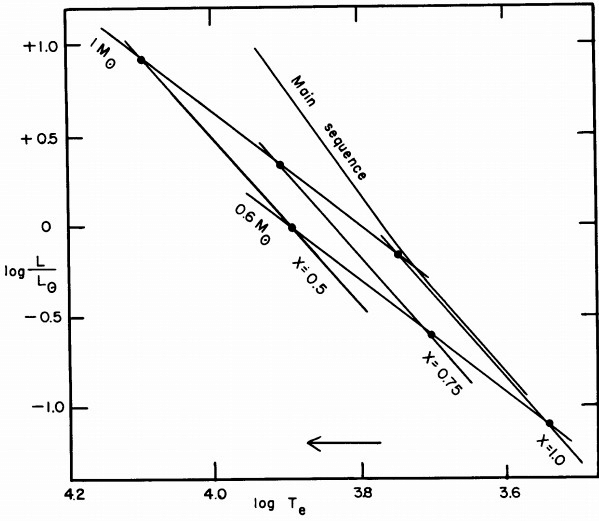
\includegraphics[width=(0.99\textwidth),height=(\textheight),keepaspectratio]{subdwarfHR}
\caption{\hr{} diagram of sub dwarf model.}
\end{figure}

\begin{figure}[!ht]
\centering
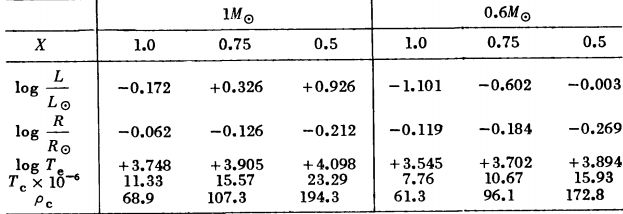
\includegraphics[width=(0.99\textwidth),height=(\textheight),keepaspectratio]{subdwarftable}
\caption{Characteristic of $0.6\msun{}$ and $1\msun{}$ sub dwarf model.}
\end{figure}

\clearpage

\subsection{Main sequence}

\begin{figure}[!ht]
\centering
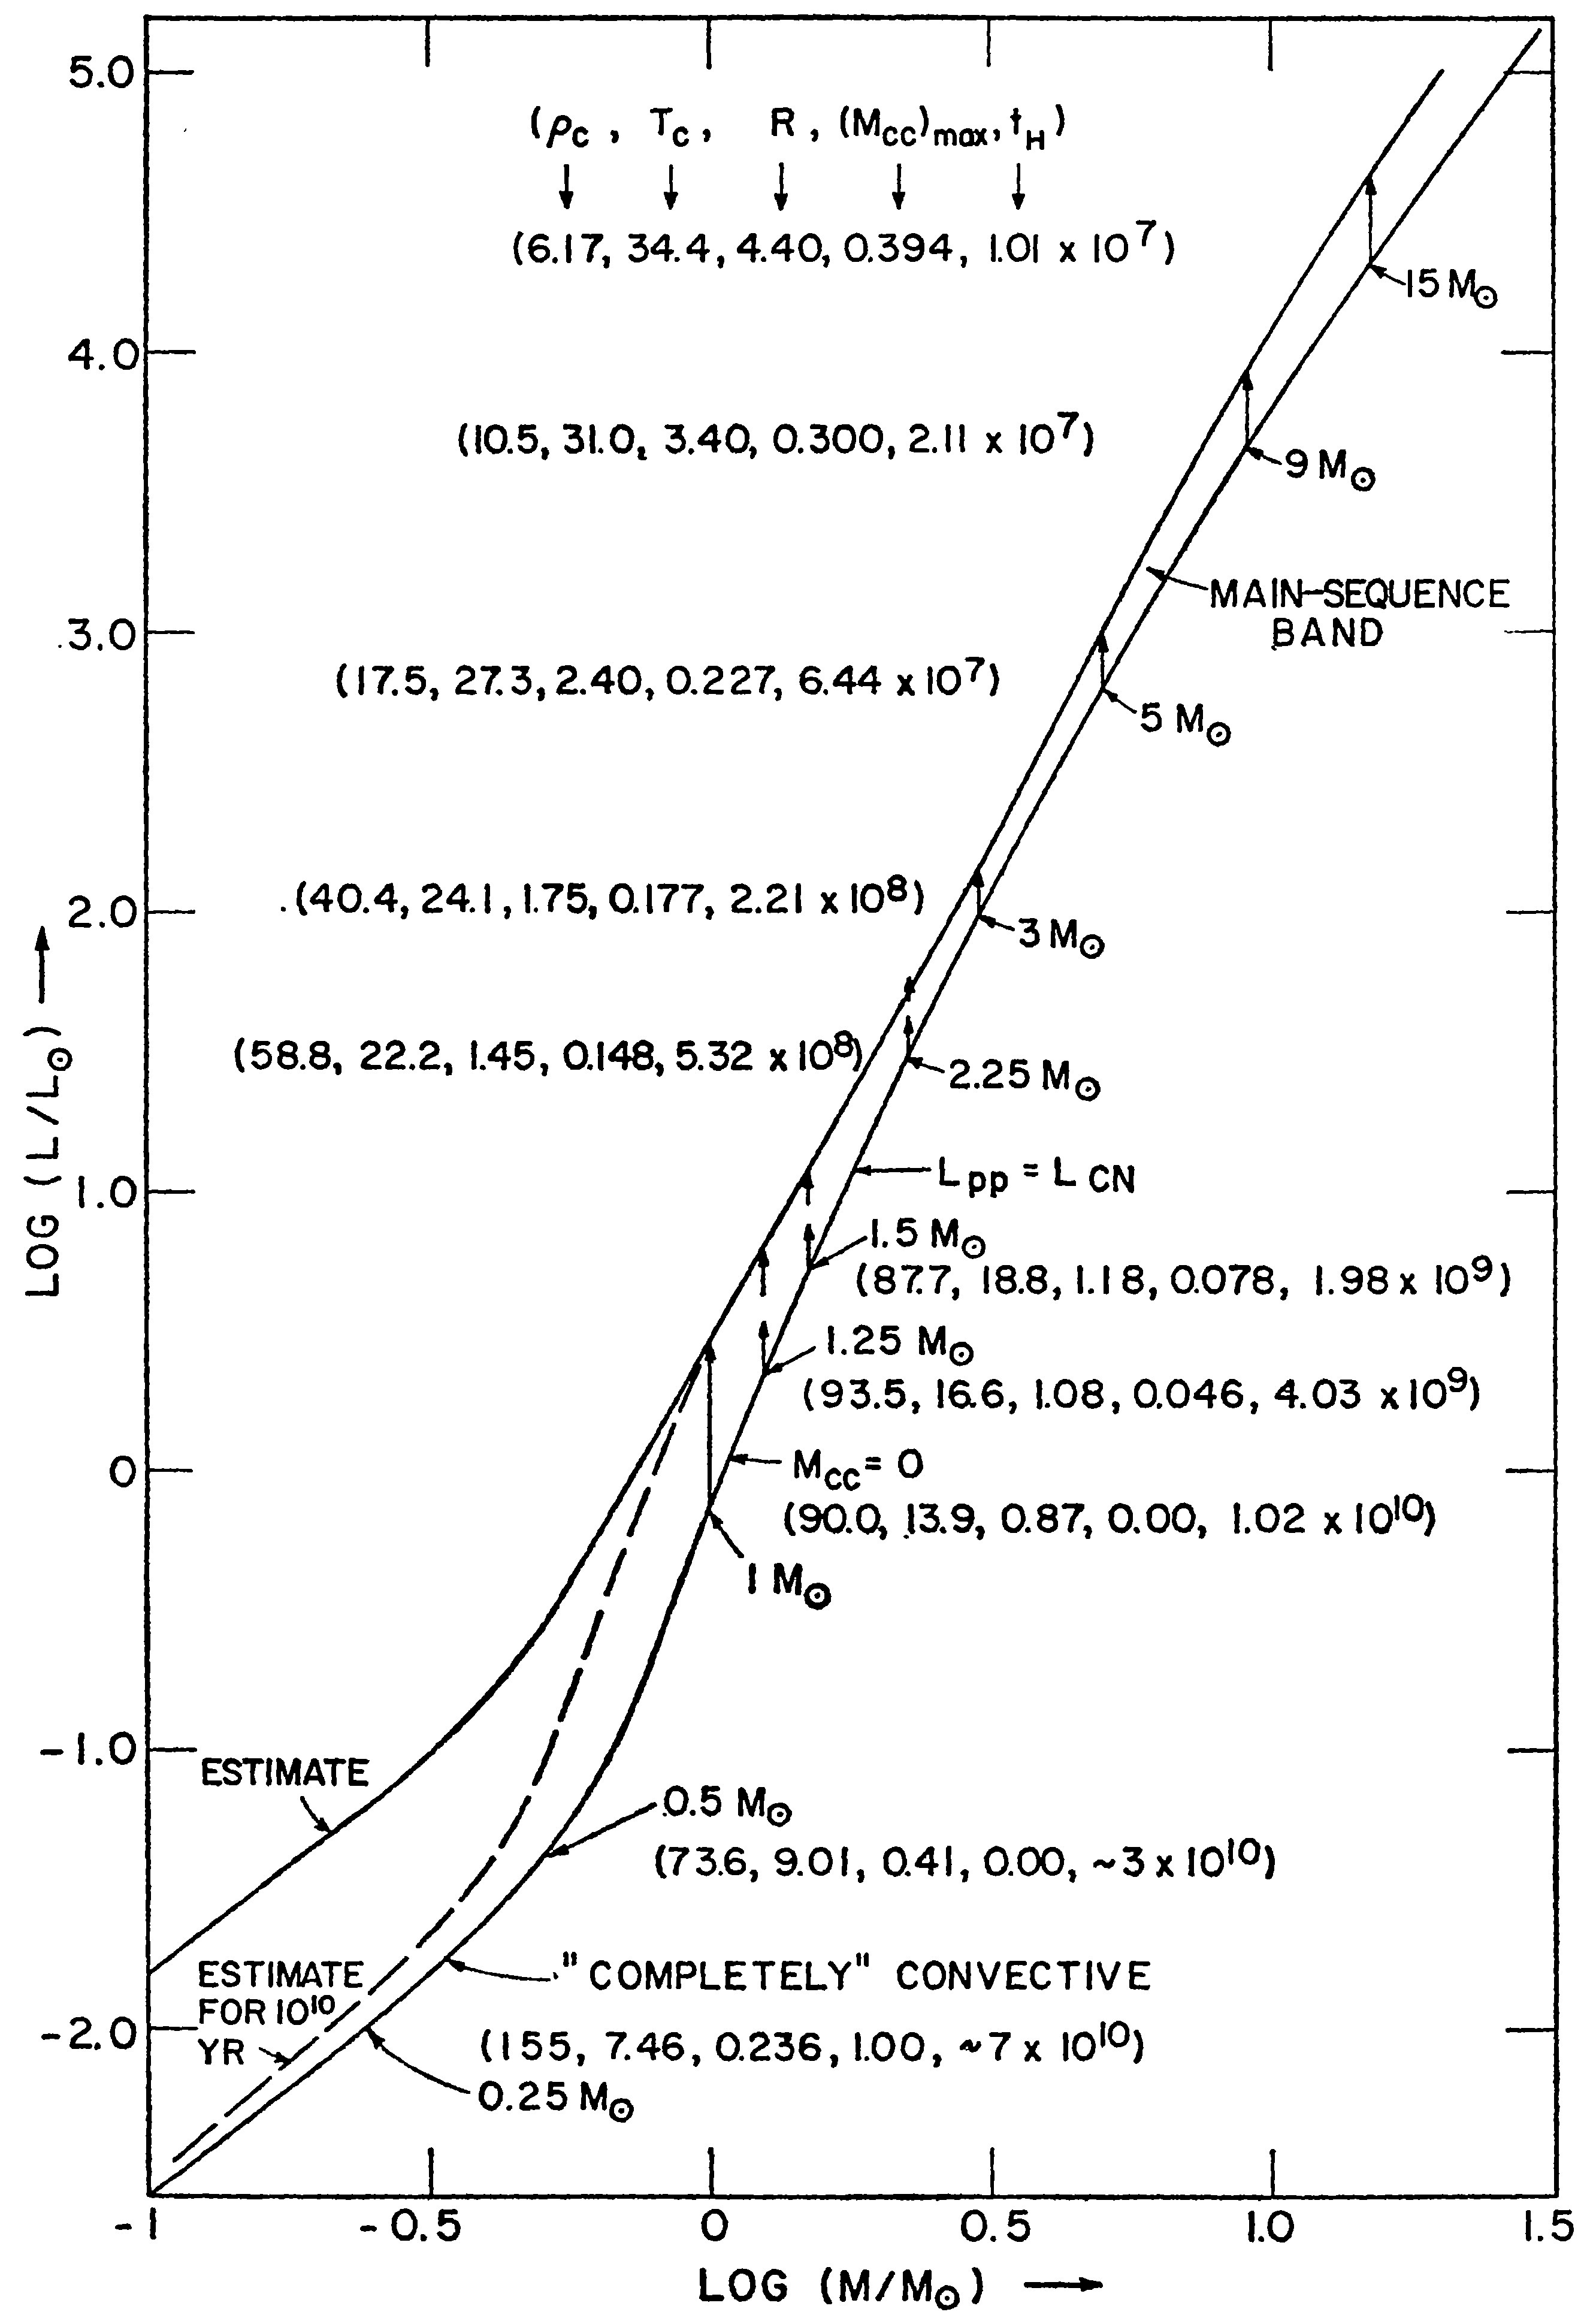
\includegraphics[width=(0.99\textwidth),height=(0.9\textheight),keepaspectratio]{MSband}
\caption{Position in M-L diagram during MS for metal rich stars. L and M are in solar units. Lower curve defines locus of homogeneous initial MS model. Number in parenthesys are \mblock{(\rho,T_6,R,\frac{M_{conv-core}^{Max}}{M},\tau_{MS})}}
\end{figure}


\clearpage

\subsection{Stellar evolution}

\begin{figure}[!ht]
\centering
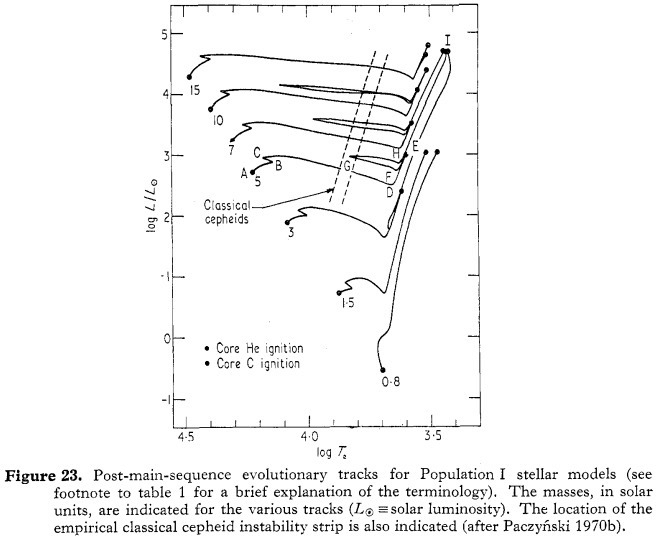
\includegraphics[width=(0.99\textwidth),height=(\textheight),keepaspectratio]{PMSevotrack}
\caption{Post MS track for population I stellar models.}
\end{figure}


\begin{figure}[!ht]
\centering
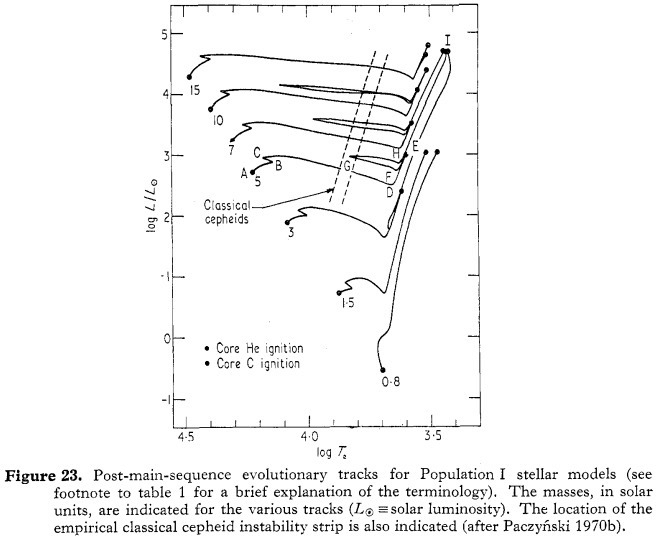
\includegraphics[width=(0.99\textwidth),height=(\textheight),keepaspectratio]{PMSevotrack}
\caption{Post MS track for population I stellar models.}
\end{figure}
ETlowmass
fiveMsunevo
evolutionMvar
timeMvar
PMSevotrack
\clearpage

\section{Composizione chimica.}

\subsection{Metallicit\'a.}
L'assenza di fusione negli strati superficiali delle stelle da dove si originano le righe fa supporre  che la loro composizione sia quella iniziale, a parte fenomeni di dredge up e sedimentazione.

La somma degli elementi pi\'u pesanti di He cresce passando da Pop. II a Pop. I.

\subsection{Formazione iniziale di metalli.}

Modelli cosmologici prevedono $Z_{in}<\num{e-6}$ mentre le stelle pi\'u vecchie osservate mostrano Z maggiore di circa 3 ordini di grandezza.

\subsection{Nucleosintesi.}
Primordial elements: they carry cosmological informations.

Prima ipotesi: decadimento di $\Pneutron\to\Pproton$ would initiates chain of neutron captures.

Von Weizsacker: nucleosynthesis in the context of stars evolutions.

Primordial fire-ball may have produced many of lightest elements but most of those with nuclear charge $Z\geq6$ are ashes of nuclear burning during stellar evolution.

Heavy elements in extreme pop II object are less abundant compared to H than they are in pop I by a factor $>100$.

He is absent in extreme popII stars.

\subsection{Galaxy chemical composition.}

If no concentration mechanism exists than the galaxy has synthetized $99\%$ of its own heavy elements.

If galaxy formed with significant abundance of He and rare elements ($D\indices{^2},He\indices{^3},Be\indices{},B\indices{}$) it must be interpreted as residual of earlier history.

\subsection{Synthesis at stellar surface.}

Non-thermal events: spallation of heavier nuclei by energetic flare particles or shock phenomena in supernovae envelopes.

\subsection{Produced in early phase of stars formations.}


\section{Fasi finali dell'evoluzione stellare.}

\subsection{Teorema del viriale}
Relazione tra l'energia cinetica media e l'energia potenziale di un sistema in equlibrio stabile o quasi-stabile.

\begin{align*}
&G=\sum_i\scap{p_i}{r_i}=\frac{1}{2}(\sum_im_ir_i^2)^2=\frac{1}{2}\frac{dI}{dt}&\intertext{I momento d'inerzia}\\
&\frac{dG}{dt}=\sum_i\scap{\dot{r_i}}{p_i}+\sum_i\scap{r_i}{\dot{p_i}}=2T\\
&+\sum_i\scap{r_i}{f_i}&\intertext{l'ultimo termi del membro di destra \'e il  viriale di Clausius}\\
&\intertext{Assumendo che la forza tra le particelle segua una legge di potenza della distanza con esponente n(del potenziale) e sia derivabile da un potenziale}\\
&\frac{dG}{dt}=2T-n\mathcal{U}&\intertext{dove U \'e l'energia potenziale totale del sistema}\\
&\frac{dG}{dt}=\frac{1}{2}\frac{d^2I}{dt^2}=2T+\Omega&\intertext{per il potenziale gravitazionale n=-1}\\
&2\overline{T}+\overline{\Omega}=0&\intertext{se il sistema \'e periodico la media del lato sinistro su un periodo dell'equazione sopra \'e nullo}
\end{align*}

\subsection{Fasi di contrazioni ed espansioni successive.}

Terminato l'idrogeno il core di elio si contrae non essendoci pi\'u fonti di energia fino a che si raggiungono T sufficienti per la fusione di dell'elio.

Detti m massa del core e r suo raggio
\begin{align*}
&E_G=-G\frac{m^2}{r}&\intertext{quindi in fase di contrazione}\\
&\Delta E_G=\frac{Gm}{r^2}\Delta r<0&\intertext{da cui risulta aumento di energia cinetica}\\
&\Delta E=-\frac{1}{2}\Delta U_G>0
\end{align*}

\subsection{fase di fusione dell'elio ($T\approx10^8K$).}

Fusione di elio-4 in carbonio-12
\begin{align*}
&^4He+^4He\to ^8_4Be\quad(\tau\approx10^{-16}s)\\
&^8Be+^4He\to^{12}C+\gamma&\intertext{al crescere di T}\\
&^{12}C+^4He\to ^{16}O+\gamma\\
&^{16}O+^4He\to^{20}Ne+\gamma
\end{align*}

\subsection{Fase di fusione del carbonio-12.}

\begin{align*}
^{12}C+^{12}C&\to ^{16}O+2^4He\\
&\to ^{20}Ne+^4He\\
&\to ^{23}Na+\Pproton\\
&\to^{24}Mg+\gamma
\end{align*}

\subsection{Fase fusione Ossigeno.}
\begin{align*}
^{16}O+^{16}O&\to ^{28}_{14}Si+^4He\\
&\to^{31}_{15}P+\Pproton\\
&\to ^{32}S+\gamma
\end{align*}

e cos\'i via fino al $^{56}Fe$ per le stelle pi\'u massicce.

\subsection{Destino finale della stella}

\begin{itemize*}
\item $M<8\msun$: Nane bianche ($R\approx R_T$).
La pressione di degenerazione degli elettroni blocca il collasso.

\item $8\msun<M<25\msun$: stella di neutroni.
La nucleosintesi raggiunge il $^{56}Fe$  poi hanno luogo fenomeni di cattura elettronica (neutronizzazione della materia): sintesi elementi pi\'u pesanti.

\item $M>25\msun$: buco nero.

\end{itemize*}


\chapter{Modelli di Stelle politropi}
\PartialToc.


\section{Polytropic gaseous spheres}

\subsection{Polytropic changes.}

\begin{definition}{Polytropic changes.}
Un elemento di materia subisce una trasformazione politropica se $dQ=cdT$ con c costante o pi\'u in generale se durante il processo di stirring la quantit\'a di calore $dQ$ fornita \'e proporzionale alla variazione istantanea di temperatura.

\begin{align*}
&(c_v-c)\,dT+P\,dV=0\\
&(c_V-c)\frac{dT}{T}+(c_p-c_V)\frac{dV}{V}=0\\
&P=K\rho\expy{\gamma'}\\
&\gamma'=\frac{c_P-c}{c_V-c}\\
&(n=-\frac{v\,dp}{p\,dv})\\
&\rho=\lambda\theta^n
\end{align*}

\end{definition}

\subsection{Limitation on stellar structure from hydrostatic equilibrium}

Impongo una relazione fra pressione e densit\'a che \'e un'idealizzazione di certe condizioni fisiche: \'e possibile separare la parte meccanica da quella termo-energetica.

\begin{align*}
&\nabla^2\Phi=4\pi G\rho&\intertext{$\uparrow$ il potenziale gravitazionale \'e soluzione dell'equazione di Poisson, che per simmetria sferica diventa:}\\
&\frac{1}{r^2}\frac{d}{dr}(r^2\frac{d\Phi}{dr})=4\pi G\rho\\
&\frac{dP}{dr}=-\frac{d\Phi}{dr}\rho=-g(r)\rho=\frac{Gm(r)}{r^2}\rho&\intertext{
Se la densit\'a non dipende dalla temperatura sostituisco la relazione $P(\rho)$ nelle equazioni meccaniche $\uparrow$}
\end{align*}

Assumo che esista una relazione del tipo
\begin{align*}
&P=K\rho^{\gamma}=K\rho^{\frac{n+1}{n}}&\intertext{ho una relazione politropa di ordine n}\\
&n=\frac{1}{\gamma-1}
\end{align*}

\subsection{Properties of solutions}

The Lane-Emden equation has a regular singularity at $z=0$:

\begin{align*}
&w(z)=1+a_1z+a_2z^2+\ldots &\intertext{con}\\
&a_1=w'(0),\quad 2a_2=w''(0),\quad\ldots &\intertext{ $a_1=0$ dato che $|\vec{g}|=\frac{d\Phi}{dr}\propto\frac{dw}{dz}$. Inserendo nell'equazione di Lane-Emden e confrontando}\\
&w(z)=1-\frac{1}{6}z^2+\frac{n}{120}z^4+\ldots &\intertext{It can be shown that for $n<5$ the radius polytropic models is finite, otherwise is infinite.}
\end{align*}

For $n<5$ the integration comes to a point where $w(z)=0$ ie $\rho=0$: the value of z, which correspons to the surface of polytrope, grows monotonically with index $n$.

One can use solution with singularity at the center for outer part of the star.

\subsection{Isothermal ideal gas.}

\begin{align*}
&\rho=\frac{\mu P}{RT}&\intertext{Per una stella isoterma di temperatura $T_0$ l'equazione di stato pu\'o essere scritta in forma di politropa }\\
&K=\frac{RT_0}{\mu}\\
&\gamma=1,\quad n=\infty
\end{align*}

\subsection{Completely convective star (Kelvin)}

Adiabatic convective equilibrium: any mass element doing convective motion is at same $T$ and $\rho$ of the surrounding.

\begin{align*}
&\nabla=(\frac{d\ln{T}}{d\ln{P}})_{ad}=\nabla_{ad}&\intertext{Per un gas completamente ionizzato e pressione di radiazione trascurabile}\\
&\nabla_{ad}=\frac{2}{5}\quad\Rightarrow\quad T\propto P^{\frac{2}{5}}&\intertext{dato che per un gas ideale con $\mu$ costante vale $T\propto\frac{P}{\rho}$ ho}\\
&P\propto\rho^{\frac{5}{3}},\quad n=\frac{3}{2}
\end{align*}

\subsection{Homogenous star}

\begin{align*}
&\rho=K_1P^{\frac{1}{\gamma}},\quad\gamma=\infty
\end{align*}

\subsection{Equazione di Lane-Emden: relazione politropica e equilibrio idrostatico.}

Hydrostatic equilibrium
\begin{equation*}
\TDy{r}{P}=-\TDy{r}{\Phi}\rho,\ (\vec{g}=-\nabla\Phi)
\end{equation*}

\begin{align*}
&\rho=\lambda\Phi^n&\intertext{Motivated by the fact that in a non degenerate polytrope of index n $\rho\propto T^n$}
&\frac{d\Phi}{dr}=-\gamma K\rho^{\gamma-2}\frac{d\rho}{dr}&\intertext{per $\gamma\neq1$ integro $\uparrow$:}\\
&\rho=(\frac{-\Phi}{(n+1)K})^n&\intertext{e sostituendo nel lato destro dell'equazione di Poisson ho:}\\
&\frac{d^2\Phi}{dr^2}+\frac{2}{r}\frac{d\Phi}{dr}=4\pi G(\frac{-\Phi}{(n+1)K})^n
\end{align*}

Introduco le variabili adimensionali
\begin{align*}
&z=Ar&\intertext{ho definito la lunghezza caratteristica tramite $\downarrow$}\\
&A^2=\frac{4\pi G}{(n+1)^nK^n}(-\Phi_c)^{n-1}\\
&=\frac{4\pi G}{(n+1)K}(\rho_c)^{\frac{n-1}{n}}&\intertext{e per il potenziale gravitazionale}\\
&w=\frac{\Phi}{\Phi_c}=(\frac{\rho}{\rho_c})^{\frac{1}{n}}&\intertext{Al centro ($r=0$) ho}\\
&z=0\\
&\Phi=\Phi_c\\
&\rho=\rho_c\\
&w=1
\end{align*}


Ora posso riscrivere l'equazione di Poisson nella forma che prende il nome da Lane e Emden
\begin{align*}
&\frac{d^2w}{dz^2}+\frac{2}{z}\frac{dw}{dz}+w^n=0\\
&\frac{1}{z^2}\frac{d}{dz}(z^2\frac{dw}{dz})+w^n=0
\end{align*}

La distribuzione radiale della densit\'a \'e

\begin{align*}
&\rho(r)=\rho_cw^n,\ \frac{\rho}{\rho_c}=\Theta^n\\
&\rho_c=[\frac{-\Phi_c}{(n+1)K}]^n\\
&P(r)=P_cw^{n+1}\\
&\left[\frac{(n+1)K_P}{4\pi G\rho_c\expy{\frac{n-1}{n}}}\right]\frac{1}{r^2}\TDof{r}(r^2\TDy{r}{\Theta})=-\Theta^n\\
&\alpha^2=[]\ (\si{\cm}),\ \xi=\frac{r}{\alpha}:\ \frac{1}{\xi^2}\PDof{\xi}(\xi^2\TDy{\xi}{\Theta})=-\Theta^n
\end{align*}

e la massa

\begin{align*}
&m(r)\int_0^r 4\pi\rho r^2\,dr=4\pi\rho_c\int_0^rw^nr^2\,dr\\
&=4\pi\rho_c\frac{r^3}{z^3}\int_0^zw^nz^2\,dz\\
&m(r)=4\pi\rho_cr^3(-\frac{1}{z}\TDy{z}{w})\, \frac{r}{z}=\frac{R}{z_n}
\end{align*}

\subsection{Dipendenza di densit\'a e pressione dalla funzione di Lane-Emden}

Assumiamo di avere una funzione $w(z)$ che soddisfa le condizioni al bordo
\begin{align*}
&w(0)=1\\
&w'(0)=0&\intertext{l'ultima $\uparrow$ deriva dall'equazione di Lane-Emden}
\end{align*}

quindi ho per pressione e densit\'a

\begin{align*}
&\rho(r)=\rho_cw^n\\
&\rho_c=(\frac{-\Phi_c}{(n+1)K})^n\\
&P(r)=P_cw^{n+1}&\intertext{con $P_c=K\rho_c^{\gamma}$.}
\end{align*}

\subsection{Relazione raggio-massa}

\begin{align*}
&R\propto M\expy{\frac{n-1}{n-3}}
\end{align*}


\section{Application to stars. Physical characteristics.}

\subsection{Polytropic model with given $n$ and $\rho_c$.}

The functions $w(z)$ and $w'(z)$ are known solutions of Lane-Emden equation

For a fixed K and n there is one-dimensional manifolds of model
\begin{equation*}
    R\propto M\expy{\frac{1-n}{3-n}}
\end{equation*}

For K as free parameter there was a 2D manifold: M and R as parameter.

\subsection{\cha{} limit mass.}

Costruisco un modello di nana bianca: core relativistico come politropa di $n=3$ con intorno un envelope non relativistico con $n=\frac{3}{2}$.

At small M the whole model is not relativistic: relativistic core occurs for $\rho_c\geq\SI{e6}{\gram\per\cubic\cm}$.

Per politropa di $n=3$ se K \'e fissato la massa non aumenta all'aumentare della densit\'a centrale, $M=C_1$:

\begin{equation*}
M=4\pi(-\frac{w'}{z})_{z_3}z_3^3(\frac{K}{\pi G})\expy{\frac{3}{2}}
\end{equation*}

Per un modello politropo di nana bianca completamente relativistica l'unica massa possibile \'e $M_{Ch}=\frac{5.836}{\mu_e^2}\msun{}$.

\section{Gravitational and total energy for polytropes}

\subsection{Gravitational energy $E_g$.}

Derivo una espressione per l'energia gravitazionale $E_g$ delle politrope:

Esplicito la dipendenza di $E_g$ dal potenziale gravitazionale $\Phi$.
\begin{align*}
&E_g=-G\int_0^M\frac{m}{r}\,dm\\
&=-\frac{1}{2}\frac{GM^2}{R}-\frac{1}{2}G\int_0^R\frac{m^2}{r^2}\,dr\\
&=-\frac{1}{2}\frac{GM^2}{R}-\frac{1}{2}\int_0^R\TDy{r}{\Phi}m\,dr\\
&=-\frac{1}{2}\frac{GM^2}{R}+\frac{1}{2}\int_0^M\Phi\,dm&\intertext{Ho usato:}\\
&\TDy{r}{\Phi}=\frac{Gm}{r^2}\quad m\Phi|_{r=0}=0\quad\Phi|_R=0
\end{align*}

Esplicito $\Phi$.

\begin{align*}
&E_g=-\frac{1}{2}\frac{GM^2}{R}+\frac{1}{6}(n+1)E_g&\intertext{$\uparrow$ ho usato:}\\
&3\int_0^M\frac{P}{\rho}\,dm=E_g&\intertext{dalla prima ricavo:}\\
&E_g=-\frac{3}{5-n}\frac{GM^2}{R}
\end{align*}

E poi per l'energia interna $E_i$:

Parametro $\xi$.
\begin{align*}
&\xi=\frac{3P}{\rho u}\\
&=3(\gamma_{Ad}-1)&\intertext{$\uparrow$ gas ideale. Questa relazione \'e vera per equazioni di stato pi\'u generali se $\xi$ \'e costante:}\\
&\xi\,du=3\frac{dP}{\rho}-3\frac{P}{\rho^2}\,d\rho&\intertext{e assumendo che i differenziali $\uparrow$ descrivano trasformazione adiabatica, cio\'e}\\
&du\,=\frac{P}{\rho^2}\,d\rho&\intertext{Infine, con}\\
&\gamma_{Ad}=\frac{\rho}{P}\TDy{\rho}{P}&\intertext{ritrovo}\\
&\xi=3\frac{\rho}{P}\TDy{\rho}{P}-3=3(\gamma_{Ad}-1)&\intertext{For ideal gas with  $\gamma_{Ad}=\frac{5}{3}$ ho $\xi=2$, for ideal gas with $\gamma_{Ad}=\frac{4}{3}$ quindi $\xi=1$.}
\end{align*}

Energia interna
\begin{align*}
&\xi E_i+E_g=0&\intertext{cio\'e}\\
&E_i=-\frac{1}{\xi}E_g=\frac{3}{\xi(5-n)}\frac{GM^2}{R}
\end{align*}

\subsection{Energia totale per stelle politrope}

\begin{align*}
&W=E_i+E_g=\frac{3}{5-n}(\frac{1}{\xi}-1)\frac{GM^2}{R}
\end{align*}

\section{Modello di Eddington}

Per un gas ideale, considerando anche la pressione di radiazion
\begin{align*}
&P=\frac{R}{\mu}\rho T+\frac{a}{3}T^4=\frac{R}{\mu\beta}\rho T&\intertext{Assumo che il rapporto $\beta=\frac{P_{Gas}}{P}$ sia costante all'interno della stella:}\\
T^4\propto P&\intertext{$\uparrow$ \'e mostrato da $1-\beta=\frac{P_{Rad}}{P}=\frac{aT^4}{3P}$. Sostituendo nell'equazione di stato ho}\\
&P=(\frac{3R^4}{a\mu^4})^{\frac{1}{3}}(\frac{1-\beta}{\beta^4})^{\frac{1}{3}}\rho^{\frac{4}{3}}&\intertext{politropa con indice $n=3$ per $\beta$ costante.}
\end{align*}

Eddington founds that the full set of stellar-structure equations (including thermo-energetic equations) could be solved very simply by the assumption $\frac{kl}{m}=const$ che implica $\beta=const$.

\section{Nane bianche}
%http://dujs.dartmouth.edu/wp-content/uploads/2008/04/09-whitedwarf.pdf
%http://upcommons.upc.edu/e-prints/bitstream/2117/18798/1/303_bravo.pdf
%http://www.astro.uvic.ca/~fherwig/TEACHING/ASTR501/StudentPresentations/EOS%20ASTR401%20MichaelP.pdf
%http://w.astro.berkeley.edu/~gmarcy/astro160/papers/physics_of_white_dwarfs.pdf

\subsection{Politropic with fixed constant}

Let's consider degenerate electron gas for which equation of state is a polytropic with  $n=\frac{3}{2}$ and
\begin{align*}
&K=\frac{1}{20}(\frac{3}{\pi})^{\frac{2}{3}}\frac{h^2}{m_e}\frac{1}{(\mu_em_u)^{\frac{5}{3}}}&\intertext{In the expression $\uparrow$ there is no room for the choice of a free parameter.}
\end{align*}

\begin{itemize*}
\item Caso NR.
\begin{equation*}
P=K_{NR}\rho^{\frac{5}{3}}\quad n=\frac{3}{2}
\end{equation*}

\item Caso R.
\begin{equation*}
P=K_{UR}\rho^{\frac{4}{3}}\quad n=3
\end{equation*}
\end{itemize*}

\subsection{Model for given $\rho_c$ and index n.}

The function $w(z)$ and $w'(z)$ are known from integration of Emden equation so
\begin{align*}
&\rho=\rho_cw^n\\
&(\frac{r}{z})^2=\frac{1}{4\pi G}(n+1)K\rho_c^{\frac{1-n}{n}}\\
&R=\frac{z_n}{A}\propto\rho_c^{\frac{1-n}{2n}}&\intertext{As long as $n>1$ the radius decreases with central density}
\end{align*}

Mass-Radius relation.

\begin{align*}
&M\propto\rho_cR^3,\ M=C_1\rho^{\frac{3-n}{2n}}&\intertext{Elimination of $\rho_c$ from the eqs above:}\\
&R\propto M^{\frac{1-n}{3-n}}
\end{align*}

There is a one dimensional manifold of model the parameter being $M$, $R$ or $\rho_c$ whereas there was two-dimensional manifold (M and R as parameter) when K was a free parameter.

\subsection{Relazione tra massa e raggio}

Equazione di Lane-Emden:
Considero l'equilibrio idrostatico
\begin{align*}
&\frac{dP}{dr}&=-G\frac{\rho(r)m(r)}{r^2}\\
&\frac{dm}{dr}&=4\pi r^2\rho(r)&\intertext{con le condizioni al contorno:}\\
&\rho(r=0)&=\rho_c,\  \rho=\frac{m_p}{Y_e}n_e=\mu_em_pn_e,\\
&\frac{1}{Y_e}=\frac{\exv{A}}{\exv{Z}}\\
&\frac{d\rho}{dr}|_0&=0
\end{align*}
\index{Peso molecolare medio elettroni}

Riscrivo l'equazione dell'equilibrio idrostatico
\begin{equation*}
\frac{d}{dr}(\frac{r^2}{\rho(r)}\frac{dP}{dr})=-G\frac{dm(r)}{dr}=-G4\pi r^2\rho(r)
\end{equation*}
e ipotizzo 
\begin{align*}
&\rho(z)=\rho_cw^n(z)&\intertext{e ho definito a con}\\
&r=az\quad a^2=\frac{(n+1)K}{4\pi G}\rho_c^{\frac{1-n}{n}}\\
&P=K\rho^{\frac{n+1}{n}}=P_cw^{n+1}(z)
\end{align*}

per trovare la pressione devo risolvere l'equazione di Lane-Emden

\begin{align*}
&\frac{1}{z^2}\frac{d}{dz}(z^2\frac{dw}{dz})=-w^n(z)&\intertext{con le condizioni al contorno}\\
&\theta(z=0)=1\quad\frac{dw}{dz}|_{z=0}=0
\end{align*}

Raggio stellare: $\rho(r=R)=0$, primo zero della $w$.
\begin{equation*}
R=az_1=B_n\rho_c^{\frac{1-n}{2n}}\quad w^n(z_1)=0
\end{equation*}

Massa stellare: $M=m(R)$.
\begin{equation*}
M=m(R)=m(a\xi_1)=\int_0^R\rho(r)4\pi r^2\,dr=A_n\rho_c^{\frac{3-n}{2n}}
\end{equation*}

Elimino la densit\'a centrale e ottendo una relazione tra massa e raggio
\begin{equation*}
M(n,R)=\frac{A_n}{B_n^{\frac{3-n}{1-n}}}R^{\frac{3-n}{1-n}}
\end{equation*}

\begin{itemize*}
\item Caso NR: $n=\frac{3}{2}$.
\begin{equation*}
M_{\frac{3}{2}}(R)\propto R^{-3}
\end{equation*}
\item Caso R: $n=3$.
\begin{equation*}
M_3(R)=const
\end{equation*}
\end{itemize*}

\begin{figure}[!ht]
\centering
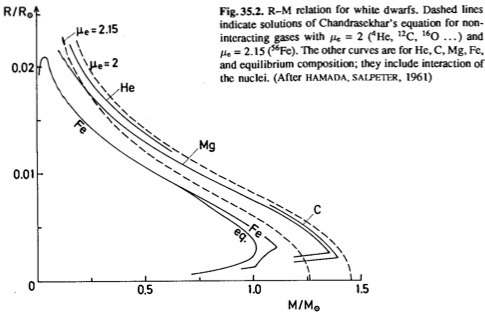
\includegraphics[width=(\textwidth-11mm),height=(\textheight-11mm),keepaspectratio]{M-R}
\caption{R-M relation for white dwarf: dashed lines indicate solution of Chandrasekhar equation for non-interacting gas with $\mu_e=2$ ($^4He$, $^{12}C$, $^{16}O$) and $\mu_e=2.15$ ($^{56}Fe$). The other are for He, C, Fe and equilibrium composition and include interactions with nuclei.}
\end{figure}


Trovo che esiste una massa limite per raggio tendente a zero e densit\'a infinita:
\begin{equation*}
M_{CSK}=M_3(R)=\frac{5.8\msun}{\mu_e^2}
\end{equation*}

\subsection{Chandrasekhar's limiting mass}

With increasing densities the electrons become gradually more relativistic: this start in the center where density is highest, the outer part remains non relativistic.

One can imagines an idealized model consisting of two regions fitted smoothly together: a relativistic polytrope core with $n=3$ surrounded by non-relativistci polytropic envelope with $n=\frac{3}{2}$.

At small mass the whole star is non-relativistic: the relativistic core will occur for $\rho_c\geq10^6\,gr/cm^3$.
For a polytrope of index $n=3$ the mass doesn't varies with central density:
\begin{align*}
M=4\pi (-\frac{w'}{z})|_{z_3}z_3^3(\frac{K}{\pi G})^{\frac{3}{2}}&\intertext{$\uparrow$ is called Chandrasekhar mass}\\
M_{Ch}=\frac{5.836}{\mu_e^2}\msun
\end{align*}

\section{Slowly rotating polytropes}

\subsection{Centrifugal acceleration from potential}

\begin{align*}
\Psi=\Phi+V&\intertext{con: }\\
\Phi=-\frac{GM}{r}\\
V=-\frac{1}{2}s^2\omega^2&\intertext{\'e possibile ricavare l'accelerazione centrifuga dal potenziale $\uparrow$. s \'e la distanza dall'asse di rotazione.}
\end{align*}

\subsection{Poisson equation for total potential}

Faccio la sostituzione $\Phi\to\Psi$: $\rho=[\frac{-\Psi}{(n+1)K}]^n
$.
\begin{align*}
\nabla^2\Psi=4\pi G\rho-2\omega^2\\
=4\pi G[\frac{-\psi}{(n+1)K}]^n-2\omega^2&\intertext{$\uparrow$ in coordinate adimensionali $y=Ar$ diventa:}\\
\Laplace_yw=w^n-\frac{\omega^2}{2\pi G\rho_c}\\
=w^n-\chi&\intertext{$\uparrow$ ho definito $\chi=\frac{\omega}{2\pi G\rho_c}$.}
\end{align*}

\subsection{Slow rotation approximation}

For $\chi\ll1$ I can approximate the solution $w(y,\theta)$ by expansion in Legendre polynomials $L_i(\theta)$:
\begin{align*}
w=w_0(y)+\chi w_1(y)+\chi w_2(y)L_2(\cos{\theta})+\ldots
\end{align*}


\chapter{Strutture autogravitanti in equilibrio: stabilit\'a rispetto a perturbazioni.}
\PartialToc


\section{Adiabatic processes: an approximation based upon physical consideration (time-scale)}

\subsection{Adiabatic evolution }
Short time-scale: adiabatic processes.
integration of equation under adiabatic condition
Properties of stellar interior under adiabatic condition

\subsection{Adiabatic exponent}

\begin{align*}
&\gamma_{ad}=\Dcvar{\PDly{\rho}{P}}{ad}&\intertext{se $\gamma_{ad}$ \'e costante, per trasformazioni adiabatiche, ho:}\\
&P\propto\rho^{\gamma_{ad}}
\end{align*}

Related to dynamical stability.

\subsection{Adiabatic temperature gradient}

\begin{align*}
&\nad=\Dcvar{\PDly{P}{T}}{ad}&\intertext{se $\nad$ \'e costante:}\\
&T\propto P^{\nad}
\end{align*}

Adiabatic temperature gradient is related to stability against convection.


\section{T. del viriale}

Chiamo U l'energia potenziale gravitazionale.

\subsection{Pressione nulla alla superficie}

\begin{align*}
&\sum_i\frac{1}{2}m_i\dvec{q_i}^2=\TDof{t}\sum_1\frac{1}{2}\vec{q_i}\dvec{q_i}-\sum_i\frac{1}{2}m_i\vec{q_i}\ddvec{q_i}&\intertext{quindi ho la prima formulazione del T  del viriale:}\\
&2E_{Kin}+U=\ddot{I}&\intertext{$\uparrow$ ho usato:}\\
&I=\sum_im_i\vec{q_i}^2\quad\ddot{I}=\TDof{t}(\sum_im_i\vec{q_i}\dvec{q_i})\\
&\sum_im_i\vec{q_i}\ddvec{q_i}=-\sum_i\vec{q_i}\nabla U=U & \intertext{$\uparrow$ sto gi\'a considerando un gas perfetto autogravitante. Se la velocit\'a e le dimensioni restano finite \'e possibile fare una media temporale:}\\
&\exv{2E_{Kin}+U}=0
\end{align*}

\subsection{Pressione esterna costante}

\begin{align*}
&\exv{2E_{Kin}+U-3PV}=0&\intertext{$\uparrow$ deriva da:}\\
&\sum_i\frac{1}{2}m_i\vec{q_i}\ddvec{q_i}\\
&=-U+\oint P\scap{r}{d\sigma}=-U+P\int_V(\scap{\nabla}{r})\,dV=\\
&-U+3PV
\end{align*}


\subsection{Pressione non omogenea}

\begin{align*}
&\exv{E_{Kin}}=\frac{3}{2}\exv{\int P\,dV}&\intertext{$\uparrow$ deriva da:}\\
&\sum_i\frac{1}{2}m_i\vec{q_i}\ddvec{q_i}=-U+\sum_i\oint_{\delta\sigma_i} P_i\scap{r_i}{d\sigma_i}\\
&=-U+\sum_i\int_{\delta V_i}\nabla(P_i\vec{r_i})\,dV_i\\
&=-U+3\int_VP\,dV+\sum_i\int_{\delta V_i}\scap{r_i}{g_i}\rho_i\,dV_i\\
&=-U+3\int_VP\,dV+\int_M\vec{r}\cdot(-\nabla\Phi)\,dm\\
&=3\int_VP\,dV
\end{align*}

Per pressione esterna nulla ho
\begin{equation*}
\exv{U}=-3\exv{\int P\,dV}
\end{equation*}


\section{Energia interna per stelle politrope. Generalizzazione del teorema del viriale.}

\subsection{Stella politropa}

\begin{align*}
&P=K\rho^{\frac{n+1}{n}}\\
&\TDy{r}{P}=-\frac{Gm(r)}{r^2}\rho(r)=-g(r)\rho(r)\\
&\PDy{r}{m}=4\pi r^2\rho(r)&\intertext{ $\uparrow$ ipotesi.}\\
&U=-G\int_0^Mm(r)\frac{\,dm}{r}\\
&=-\frac{GM^2}{2R}-G\int_0^R\frac{m^2(r)}{2r^2}\,dr&\intertext{Usando $\frac{dP}{\rho}=(n+1)d(\frac{P}{\rho})$:}\\
&U=-\frac{GM^2}{2R}+\frac{n+1}{2}\int m(r)\,d(\frac{P}{\rho})\\
&=-\frac{GM^2}{2R}+\frac{n+1}{2}\overbrace{\int_0^M\,d(\frac{mP}{\rho})}^{\approx0,\quad\frac{P}{\rho}\propto T}\\
&-\frac{n+1}{2}\int_0^M\frac{P}{\rho}\,dm&\intertext{Ho quindi:}\\
&U=-\frac{GM^2}{2R}-\frac{n+1}{2}\int P\,dV\\
&=-\frac{GM^2}{2R}+\frac{n+1}{6}U&\intertext{L'energia potenziale gravitazionale \'e:}\\
&U=-\frac{3}{5-n}\frac{GM^2}{R}
\end{align*}

\begin{comment}
\begin{tikzpicture}[overlay, remember picture]
\draw [decoration={brace,amplitude=0.5em,mirror},decorate,ultra thick,red] (first.north) -- (second.south) node[midway,label={[label distance=1mm]-100:Ipotesi}] {};
\end{tikzpicture}
\end{comment}
\index{Re-use: Tikzmark}

\subsection{Calcolo energia interna: stella politropa adiabatica.}

Densit\'a di energia interna.
\begin{align*}
&P=\alpha\rho^{1+\frac{1}{n_{AD}}}&\intertext{Esplicito la dipendenza dell'energia interna da $P$ e $\rho$ usando la condizione di adiabaticit\'a:}\\
&(dE+P\,dV=0,\ V=Mv=\frac{M}{\rho},\  E=e_IM)\\
&e_I\propto\rho^{\delta}P^{\xi}=\beta\rho^{\theta}\\
&(P=-\left.\frac{\partial E}{\partial V} \right|_{S,A}=-\frac{\partial (\frac{E}{A})}{\partial (\frac{V}{A})}\\
&=-\frac{\partial \epsilon}{\partial \frac{1}{\rho}}=\rho^2 \frac{\partial \epsilon}{\partial \rho})\\
&P=-(\PDy{V}{E})_S\xrightarrow{\rho=\frac{1}{v}}\rho^2(\TDy{\rho}{e_I})_S=\theta\beta\rho^{\theta+1}&\intertext{quindi ricavo gli esponenti:}\\
&\theta_{AD}=\frac{1}{n_{AD}}\quad\beta=\frac{\alpha}{\theta}=\alpha n_{AD}&\intertext{Gas perfetto monoatomico $\downarrow$}\\
&n_{AD}=\frac{3}{2}&\intertext{Gas di radiazione $\downarrow$}
&n_{AD}=3\\
&e_I=n_{AD}\frac{P}{\rho}
\end{align*}

\subsection{Generalizzazione del teorema del viriale: tengo conto dell'energia interna (solo termica).}

\begin{align*}
&\int P\,dV=\frac{1}{n_{Ad}}\int e_I\rho\,dV\\
&=\frac{1}{n_{Ad}}\int e_i\,dM=\frac{1}{n_{Ad}}E_{Int}&\intertext{$\uparrow$ ho integrato $e_I=n_{Ad}\frac{P}{\rho}$ in $dV$. Utilizzando:}\\
&\exv{U}=-3\int P\,dV&\intertext{ottengo}\\
&E_{Int}=-\frac{n_{Ad}}{3}U
\end{align*}

Infine ho una relazione fra l'energia totale $E$ e l'energia potenziale gravitazionale (dipendente dall'indice adiabatico e da quello politropico) se $\xi=3\frac{\rho}{P}\TDy{\rho}{P}-3=3(\gamma_{Ad}-1)$ \'e costante in tutta la stella:
\begin{align*}
&E=E_{Int}+U=\frac{3-n_{Ad}}{3}U=\frac{3-n_{Ad}}{5-n}\frac{GM^2}{R}&\intertext{ che nel caso di una struttura convettiva ($n=n_{Ad}$) diventa:}\\
&E=-\frac{3}{7}\frac{GM^2}{R}
\end{align*}



\section{Criterio di stabilit\'a}

\subsection{Perturbazione adiabatica}

Perturbazione self-similar: \mblock{r\to r+\delta r=(1+\alpha)r}.
\begin{align*}
&v=\frac{1}{\rho}\to(1+\alpha)^3v,\quad\,dv\to(1+\alpha)^3\,dv&\intertext{quindi al secondo ordine in $\alpha$ ho:}\\
&\delta v=(3\alpha+3\alpha^2)v,\quad (\delta v)^2=(3\alpha)^2v^2,\\
&\rho\to(1+\alpha)^{-3}\rho,\\
&M\to M\\
&-P=\PDy{v}{e_I}&\intertext{$\uparrow$ primo principio $dq=/,du+P\,dv$ per trasformazioni adiabatiche}\\
&\gamma_{Ad}\frac{P}{v}=-\Dcvar{\PDy{v}{P}}{Ad}=\Dcvar{\TtwoDy{v}{e_I}}{Ad}&\intertext{La prima ugaglianza di $\uparrow$ deriva dalla definizione di $\gamma_{Ad}=\Gamma_{Ad}=\Dcvar{\TDly{\rho}{P}}{Ad}$, la secando uguaglianza dalla sostituzione della prima equazione.}
\end{align*}

Determino la variazione di energia al secondo ordine in $\alpha$:
\begin{align*}
&E=\int\,dM[e_I-\frac{GM(r)}{r}]\\
&e_I\to e_i+\Dcvar{\PDy{v}{e_I}}{Ad}\delta +\frac{1}{2}\Dcvar{\PtwoDy{v}{e_i}}{Ad}(\delta v)^2&\intertext{$\uparrow$ primo principio}\\
&\approx e_I-Pv(3\alpha+3\alpha^2)\\
&+\frac{1}{2}\Gamma_{Ad}\frac{P}{v}(3\alpha)^2v^2&\intertext{da cui:}\\
&E=\int\,dM[e_I-Pv(3\alpha+3\alpha^2)\\
&+\frac{1}{2}\Gamma_{Ad}\frac{P}{v}(3\alpha)^2v^2\\
&-\frac{1}{1+\alpha}\frac{GM}{r}]\\
&\delta E=\int\,dV[\alpha(-3P+\frac{GM(r)}{r}\rho)\\
&+\alpha^2(-3P+\frac{9}{2}\Gamma_{Ad}P-\frac{GM(r)}{r}\rho)]
\end{align*}


\subsection{Condizione di stabilit\'a}

La condizione di equilibrio \'e data dall'annullarsi del coefficiente lineare in $\alpha$:
\begin{equation*}
3\int\,dV=\int\frac{Gm(r)\rho}{r}\,dV=-U
\end{equation*}
La condizione di stabilit\'a \'e data dalla positivit\'a della derivata seconda
\begin{align*}
&\int\,dV[-3P+\frac{9}{2}\Gamma_{Ad}P-\frac{GM\rho}{r}]>0\\
&\int(\Gamma_{Ad}-\frac{4}{3})P\,dV>0
\end{align*}

\subsection{Perturbazione di ampiezza finita}

Dipendenza della pressione dalla densit\'a in condizioni di equilibrio
\begin{align*}
&P\propto GM^{\frac{2}{3}}\overline{\rho}^{\frac{4}{3}}(R)&\intertext{$\uparrow$ ricavata da:}\\
&Const\,GM^{\frac{2}{3}}\overline{\rho}^{\frac{4}{3}}(R)\leq P_c\leq\,Const\,GM^{\frac{2}{3}}\rho_c^{\frac{4}{3}}\\
&\frac{\delta P}{P}=\frac{4}{3}\frac{\delta\rho}{\rho}
\end{align*}

Perturbazione Adiabatica:
\begin{align*}
&\frac{\delta P}{P}=\Gamma_{Ad}\frac{\delta\rho}{\rho}\\
&P=P_0(\frac{\rho}{\rho_0})^{\Gamma_{Ad}}&\intertext{$\Gamma_{Ad}$ costante, $(P_0,\rho_0)$ condizione di equilibrio, con:}\\
&P_0=AGM^{\frac{2}{3}}\rho_0^{\frac{4}{3}},\quad A\approx1 &\intertext{Descrivo una perturbazione adiabatica con:}\\
&P(\rho)=P_0(\frac{\rho}{\rho_0})^{\Gamma_{Ad}}=(1-F)AGM^{\frac{2}{3}}(\frac{\rho}{\rho_0})^{\frac{4}{3}}\rho_0^{\frac{4}{3}}&\intertext{dalla condizione di equilibrio ho:}\\
&P(\rho)=(1-F)(\frac{\rho}{\rho_0})^{\frac{4}{3}}P_0&\intertext{confrontando le due equazioni ricavo:}\\
&1-F=(\frac{\rho}{\rho_0})^{\Gamma_{Ad}-\frac{4}{3}}&\intertext{se a causa di una perturbazione ho $\rho>\rho_0$, $\uparrow$ implica}\\
&\intertext{Per $\Gamma_{Ad}>\frac{4}{3}$, la densit\'a tende verso il valore di equilibrio. Ho l'equazione del moto radiale per un guscio sferico:}\\
&\TtwoDy{t}{r}=-F\frac{Gm(r)}{r^2}>0&\intertext{$\uparrow$ perch\'e $F<0(1-F>1)$.}\\
&\intertext{Per $\Gamma_{Ad}<\frac{4}{3}$, la densit\'a diverge dal valore di equilibrio. Ho l'equazione del moto radiale per un guscio sferico:}\\
&\TtwoDy{t}{r}=-F\frac{Gm(r)}{r^2}<0&\intertext{$\uparrow$ perch\'e $F>0(1-F<1)$.}
\end{align*}

Per $\Gamma_{Ad}>\frac{4}{3}$ la pressione cresce/diminuisce troppo rapidamente all'aumentare/diminuire di $\rho$ bloccando la contrazione/espansione.

Per $\Gamma_{Ad}>\frac{4}{3}$ la perturbazione \'e destinata a crescere.

\section{Problema delle pulsazioni.}


\subsection{Pulsazioni radiali: modello elementare}
vedi cox

\subsection{Effetto della perturbazione sull'energia: secondo ordine.}

Per $\Gamma_{Ad}<\frac{4}{3}$ una perturbazione pu\'o essere amplificata esponenzialmente 
\begin{align*}
&v\to(1+\alpha)^3v,\quad \frac{\delta r}{r}=\frac{\delta R}{R}=\alpha\\
&E=\int\,dm[e_I-\frac{Gm(r)}{r}]\\
&\delta E\approx\alpha^2\underbrace{\int\,dV(-3P+\frac{9}{2}\Gamma_{Ad}P-\frac{Gm(r)\rho}{r})}_{=\frac{3}{2}\int\,dVP(3\Gamma_{Ad}P-4)=-\frac{U}{2}\exv{4\Gamma_{Ad}-4}}&\intertext{Posto $-U=\xi\frac{GM^2}{R}$, dove $\xi\approx1$, riscrivo}\\
&\delta E\approx\frac{1}{2}\xi\frac{GM^2}{R}\exv{(3\Gamma_1-4)(\frac{\delta r}{r})^2}
\end{align*}

\subsection{Periodo di pulsazione}

\begin{align*}
&\omega^2=\frac{K'}{M}=\xi G\frac{M}{R^3}\exv{3\Gamma_1-4}\\
&=\frac{4}{3}\xi\pi G\overline{\rho}\exv{3\Gamma_1-4}\\
&\tau_{Puls}=\frac{2\pi}{\omega}\approx t_{ff}&\intertext{$\uparrow$ se $\exv{3\Gamma_1-4}$ \'e abbastanza lontano da zero.}
\end{align*}

\subsection{Relazione Periodo-Luminosit\'a}

\begin{align*}
&\frac{\tff}{\tkh}\approx\frac{\Pi}{\tkh}\approx\frac{LR^{\frac{5}{2}}}{G^{\frac{3}{2}}M^{\frac{5}{2}}}\approx\sci{-12}\frac{LR^{\frac{5}{2}}}{M^{\frac{5}{2}}}\\
&L\propto M^{\frac{2}{3}}T_e^4t_{puls}^{\frac{4}{3}}&\intertext{$\uparrow$ la temperatura effettiva \'e definita da:}\\
&L=4\pi R^2aT_e^4
\end{align*}

\subsection{Zone di ionizzazione parziale}

La teoria delle stelle pulsanti mette in evidenza l'importanza delle zone di ionizzazione parziale.




\chapter{Nane bianche}
\PartialToc

\section{Spectra of white dwarf}

Lines in spectra of white dwarf are strongly broadened by pressure effects: the wings of hydrogen lines overlap.

\subsection{Statistical Stark effect}

conditions under which hydrogen lines merge into the continuum, disappearance of higher quantum states and formation of continuus spectrum.

\section{Internal constitution}


\section{Physical properties of dense matter}

\end{document}

\part{Osservabili stellari. Classificazione}


\chapter{Massa, distanza, raggio e luminosit\'a. Fotometria, astrometria.}
\PartialToc

\section{Generalit\'a sull'astronomia sferica.}

\subsection{Sfera celeste}

\begin{figure}[!ht]
\centering
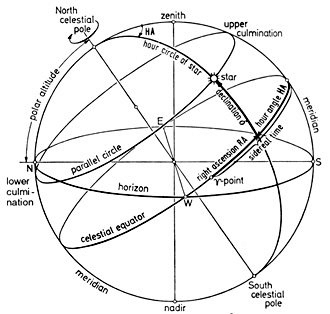
\includegraphics[width=(\textwidth),height=(\textheight-11mm),keepaspectratio]{CelestialSphere}
\caption{Sfera celeste.}
\end{figure}

\subsection{Declinazione e ascensione retta}



\clearpage


\subsection{Radio resonance in atomic and nuclear system.}

\subsection{Phase of the Earth respect distant stars}

Intersection of equatorial plane of the ecliptic at fixed epoch: $\gamma$-point. Instead of the angle $\phi$ one often uses the Universal Time
\begin{equation*}
UT1(t)=\frac{\phi(t)}{\omega_0}
\end{equation*}

\subsection{Standard for length has been forgone. Definition of speed of light.}

Tradizionalmente l'unit\'a di lunghezza, centimetro, si definisce tramite misure interferometriche come multiplo della lunghezza d'onda $\lambda_0$ di  una linea ottica stabile. \'E possibile misurare la velocit\'a della luce misurando la frequenza $\frac{c}{\lambda_0}$ tuttavia si preferisce \underline{definire} la velocit\'a della luce, se $c=1$ le lunghezze son misurate in secondi luce. This is appropriate to space physics in which distances are usually measure with transit time of light or radio pulses, timed by atomic clocks, or by means of doppler effect. In both cases only time standard is used. Inoltre la teoria della relativit\'a ci dice che lo spazio e il tempo sono uniti geometricamente in uno stesso concetto.

Time and frequency can by transerred from one point to another by EM signals
\begin{align*}
\frac{\nu_2}{\nu_1}=\overbrace{\sqrt{\frac{1-(\frac{v_1}{c})^2}{1-(\frac{v_2}{c})^2}}}^{\text{\hspace*{0pt} Transversal Doppler effect}}\underbrace{\frac{1-\frac{\vec{v_2}\cdot\hat{k}}{c}}{1-\frac{\vec{v_1}\cdot\hat{k}}{c}}}_{\text{\hspace*{0pt} ordinary Doppler effect}}
\end{align*}

%\subsection{Misure di parallasse}

\section{Keplerian problem}

\subsection{Prima legge di Keplero}

Sotto l'azione di una forza attrattiva un corpo celeste si sposta nel campo di attrazione dell'altro corpo celeste secondo una sezione conica: cerchio, ellisse, parabola, iperbole

\begin{usefull}{Prima legge di Keplero: consequence of inverse law of gravity.}
The orbit of a planet is an ellipse with the Sun at one focus.

For general two-body problem where the mass of secondary is not neglected both orbits are ellipses with their foci at their common barycentre
\end{usefull}

\subsection{Seconda legge di Keplero}

\begin{align*}
&m\TDof{t}(x\TDy{t}{y}-y\TDy{t}{x})=xF_y-yF_x&\intu{segue da legge fondamentale della dinamica newtoniana,}\\
&\TDof{t}(x\TDy{t}{y}-y\TDy{t}{x})=0&\intu{considerazioni geometriche implicano $\frac{F_x}{F_y}=\frac{x}{y}$.}\\
&x=r\cos{\theta},\quad y=r\sin{\theta}\\
&r^2\TDy{t}{\theta}=const&\intu{le aree spazzate dal raggio vettore nell'unit\'a di tempo sono una costante.}
\end{align*}

\begin{usefull}{Seconda legge di Keplero: conservation of angular momentum.}
The line joining a planet and the Sun sweeps out equal areas in equal intervals of time.

\end{usefull}

\subsection{Terza legge di Keplero}


Uguagliando le accelerazioni del moto circolare di velocit\'a angolare $\omega=\frac{2\pi}{T}$, $\omega^2r=\frac{4\pi^2r}{T^2}$, e dell'attrazione gravitazionale $G\frac{M+m}{r^2}$ si ottiene
\begin{equation*}
\frac{r^3}{T^2(M+m)}=\frac{G}{4\pi^2}=const
\end{equation*}

Per due corpi di massa $m_1$ e $m_2$ con semiasse maggiore delle rispettive orbite $a_1$ e $a_2$ e periodo $T_1$ e $T_2$
\begin{align*}
&\frac{a_1^3}{T_1^2(M_1+m_1)}=\frac{G}{4\pi^2}\\
&\frac{a_2^3}{T_2^2(M_2+m_2)}=\frac{G}{4\pi^2}\\
&\frac{T_1^2(M_1+m_1)}{T_2^2(M_2+m_2)}=\frac{a_1^3}{a_2^3}\\
&\frac{T_1^2}{T_2^2}=\frac{a_1^3}{a_2^3}&\intu{terza legge di Keplero ($M_1=M_2$, $m_1\approx m_2=0$).}
\end{align*}

\begin{usefull}{Terza legge di Keplero: inverse law of gravity}
The squares of the orbital periods of the planets are proportional to cubes of their semi-major axis.
\end{usefull}


\subsection{Orbite relative}

For general two-body problem where the mass of secondary is not neglected both orbits are ellipses with their foci at their common barycentre. La terza legge si riscrive
\begin{equation*}
P^2=\frac{4\pi^2}{GM}a^3
\end{equation*}

Il moto del pianeta relativo alla stella invece che al baricentro pu\'o essere trovato applicando un'accelerazione al sistema che cancella quella della stella (\mblock{\frac{Gm_p}{r^2}}), quindi la terza legge si riscrive

\begin{equation*}
P^2=\frac{4\pi^2}{G(M_*+M_p)}a_{rel}^3
\end{equation*}


Fatti:
\begin{itemize}
\item The measurements of relative separation doesn't arise for exoplanet orbit when the planet is unseen.

\item For binary star where an orbit is measured as a separtion and position angle of one star with respect another, the the combined system mass can be determined if $P$ and $a_{rel}$ are measurable. Individual masses can only be determined if mass ration can be established: from ratio of distances from barycentre or ratio of their speed around it.

\end{itemize}

For $m_p\ll M_*$ (in units of Earth's orbit of \SI{1}{\astronomicalunit})

\begin{equation*}
P\approx\SI{1}{\year}(\frac{a_{rel}}{\si{\astronomicalunit}})\expy{\frac{3}{2}}(\frac{M_*}{\msun{}})\expy{-\frac{1}{2}}
\end{equation*}

\subsection{Absolute orbits}

The orbit of the star around system star-planet barycentre is given by
\begin{align*}
&P^2=\frac{4\pi^2}{GM'}A_*^3\\
&M'=\frac{m_p^3}{(M_*+m_p)^2}&\intu{$a_*$ is the semi-major axis of stellar orbit around system barycentre}\\
&a_*:a_p:a_{rel}=m_p:M_*:(M_*+m_p)\\
&a_{rel}=a_*+a_p\\
&e_{rel}=e_*=e_p,\ P_{rel}=P_*=P_p\\
\end{align*}

Stellar position vs time allows maximum and minimum angular rate to be detrmined and hence positions of line of apsides: with orientation of orbit so determined appeal's to Kepler second law fixes orbit inclination.

Radial velocity measurement of host star gives informations on its barycentric orbital motion.

\section{Orbit specification}

A keplerian orbit in 3D is described by $a$, $e$ which specify the size and shape of elliptical orbit and $P$ related to $a$ and component masses through Kepler law, $t_p$ which is the position of the planet along its orbitat a particular reference time, and the three angle \mblock{(i,\Omega,\omega)} which represent the projection of true orbit into observed apparent orbit.



\tpc{!ht}{

\node at (0,0) {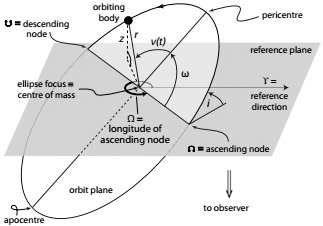
\includegraphics[width=(0.9\textwidth),height=(\textheight),keepaspectratio]{3Dorbit}};

\node at (0,-5) {\parbox{0.9\textwidth}{The reference plane is tangential to celestial sphere, i is the inclination of orbit plane. The true anomaly $\nu(t)$ is the time-dependent angle characterizing the object position along the orbit.}};
}
{(0,-6)}{6cm}{Elliptical orbit in 3D.}

\section{Luminosity function} 

\subsection{Trigonometric parallax}

Stars near the sun: object with total proper motion $\mu>\mu_0$

\subsection{spectroscopic parallax}

To apply this method, one must measure the apparent magnitude of the star and know the spectral type of the star. If the star lies on the main sequence, the spectral type of the star provides a good estimate of the star's absolute magnitude. Knowing the apparent magnitude (m) and absolute magnitude (M) of the star, one can calculate the distance (d, in parsecs) of the star using
\begin{align*}
&M − m = − 5\log{\frac{d}{10}}    
\end{align*}
The true distance to the star may be different than the one calculated due to interstellar extinction.

The spectroscopic absolute magnitude $M$ are derived from the intensity ratio of a number of Fraunhofer lines: the spectroscopic parallax are found using
\begin{equation*}
M=m+5+5\log{\pi_s}-a(\pi_s)
\end{equation*}

\subsection{Comparison of distribution of proper motion components and tangential}



\section{Indicatori di distanza.}

\subsection{Parallasse}

Le coordinate dei corpi celesti osservati dalla superficie terrestre sono topocentriche: la differenza tra diversi punti di osservazione sulla superficie terrestre non \'e trascurabile solo per i corpi del sistema solare e per stelle inferiori a \ang{;;0,00004} essa praticamente non esiste.

Fra le moltitudini di direzioni in cui l'astro \'e visibile dalla superficie quella principale \'e quella con origine nel centro della terra: fornisce la posizione geocentrica dell'astro e determina le sue coordinate geocentriche. L'angolo tra le direzioni secondo cui l'astro $M'$ sarebbe visibile da un qualsiasi punto sulla superficie e dal centro della Terra si chiama parallasse diurna: \'e l'angolo $p'$ sotto il quale dall'astro si vede il raggio della terra per il luogo di osservazione. La parallasse di un astro allo zenit nell'istante di osservazione \'e nulla, se l'astro \'e osservato all'orizzonte la sua parallasse diurna \'e massima ed \'e allora detta parallasse orizzontale $p$.


\subfile{tikz/diurnalparallax.tex}


La relazione fra i lati e gli angoli dei triangoli $TOM'$ e $TOM$ d\'a
\begin{align*}
&\frac{R}{\Delta}=\frac{\sin{p'}}{\sin{z'}},\quad \frac{R}{\Delta}=\sin{p}\\
&\sin{p'}=\sin{p}\sin{z'}
\end{align*}
 La parallasse orizzontale di tutti i corpi del sistema solare \'e molto piccola: Luna $p=\ang{;57;}$, Sole $p=\ang{;;8.79}$, per i pianeti \'e inferiore ad un primo.

I seni delle parallassi possono essere sostituiti con gli angoli stessi: $p'=p\sin{z'}$. 

Poich\'e la forma della Terra \'e quella di uno sferoide si definisce come raggio standard il raggio equatoriale $R_0=6379\si{\kilo\meter}$ e le parallassi orizzontali calcolate per questo raggio si chiamano parallassi orizzontali equatoriali $p_0$.


\subsection{Parallasse.}

Si misura lo spostamento della stella rispetto ad un riferimento di stelle fisse: parallasse diurna $\Delta T=1 \si{\hour}$ (sistema solare), parallasse annua $\Delta T$ di 6 mesi.


\begin{equation*}
    \pi_d=\frac{O_1O_2}{r}=\frac{2r_T\cos{\phi}}{r}
\end{equation*}
cio\'e l'angolo sotteso dalla distanza tra i due punti di osservazione visto dalla stella.

\begin{definition}{Parsec}
Distanza alla quale il semi-asse maggiore dell'orbita terrestre sottende:

\SI{1}{\arcsec}.

\end{definition}

Fatti:
\begin{itemize}
    \item Le stelle pi\'u vicine sono distanti qulache parsec.
    \item Potere risolutivo di un telescopio: $\frac{D}{\lambda}$. Per D=\SI{1}{\meter} e $\lambda=\SI{5000}{\angstrom}$ ho un potere risolutivo di \SI{0.1}{\arcsec}.
    \item Thecniche di best-fit: Numerose osservazioni vs ellissi teorica.
    \item Le osservazioni terrestri sono limitate dal seeing.
\end{itemize}

\subsubsection{Distanze corpi celesti.}

Conoscendo la parallasse equatoriale orizzontale $p_0$ dell'astro si calcola la sua distanza dal centro della terra
\begin{align*}
&\Delta=\frac{R_0}{\sin{p_0}}\\
&\sin{p_0}=p_0''\sin{\ang{;;1}}=\frac{p_0''}{\ang{;;206265}}\\
&\Delta=\frac{\ang{;;206265}R_0}{p_0''}&\intertext{$\uparrow$ le parallassi sono molto piccole: fornisce le distanze dei membri del sistema solare.}
\end{align*}
La distanza del corpo celeste \'e ottenuta nelle stesse unit\'a del raggio  della terra $R_0$.


\subsubsection{Parallasse annua.}

L'angolo sotto cui da una stella si vedrebbe il raggio medio dell'orbita terrestre nella condizione che la direzione verso questa stella sia perpendicolare a questo raggio si chiama parallasse annua $\pi$.

\begin{align*}
&\Delta=\frac{a}{\sin{\pi}}&\intertext{a \'e il raggio medio dell'orbita terrestre. Le parallassi delle stelle sono inferiori a \ang{;;1}:}\\
&\Delta=\frac{\ang{;;206265}a}{\pi''}
\end{align*}

Le parallassi determinate in base allo spostamento parallattico dell'astro sono dette trigonometriche. Le parallasi sono misurate con sufficiente precisione se la loro distanza non supera i 100\si{\parsec} ($\pi=\ang{;;0.01}$): si conoscono le parallassi di circa 6000 stelle vicino al sole.

\subsection{Moto proprio}

Spostamento progressivo rispetto ad un sistema stelle fisse (Blinking): proper motion is the astronomical measure of the observed changes in apparent positions of stars in the sky as seen from the center of mass of the Solar System compared to the imaginary fixed background of the more distant stars.

 This transverse sky motion is separate from the radial velocity, being the velocity moving toward or away from the observer in kilometres per second ($km/s$), as obtained from the Doppler shifts in starlight seen with a spectroscope. Knowledge of the proper motion, distance, and radial velocity allow approximate calculations of a star's true motion in space in respect to the Sun.

Stima distanza:
il moto proprio \'e inversamente proporzionale alla distanza, si deve ipotizzare la conoscenza della velocit\'a relativa rispetto al Sole V. Ipotizzando V costante per stelle vicine e uguale alla velocit\'a del Sole nell'ambiente locale trovo una relazione tra moto proprio sulla sfera celeste u, parallasse e velocit\'a sulla sfera celeste $V_0\sin{\lambda}$ con $\lambda$ angolo tra congiungente stella Sole e direzione del moto del Sole.

\begin{align*}
    &u=\frac{V_0\sin{\lambda}}{4.74}\pi&\intertext{$V_0$ in \si{\kilo\meter\per\second}}\\
    &H=\frac{\pi V_0}{4.74}&\intu{Parallasse secolare}
\end{align*}

Fatti:
\begin{itemize}
    \item Stelle vicine.
    \item Moto proprio progressivo.
    \item Ipotesi V costante applicabile a gruppo di stelle. Parallasse media: 
    \begin{equation*}
        \pi_{media}=\frac{4.74\sum u_i}{V_0\exv{\sin{\lambda}}N}
    \end{equation*}
\end{itemize}

\subsection{Parallasse di gruppo}

Associazione fisica di stelle con stessa velocit\'a relativa rispetto al sole
\begin{equation*}
    V=V_r\hat{r}+V_T\hat{e_T}
\end{equation*}
$V_T$ \'e osservabile mediante effetto Doppler, $V_T$ \'e legata al moto proprio. La parallasse di gruppo \'e 
\begin{equation*}
    \pi_{Gruppo}=\frac{4.74u}{V_R\tan{\lambda}}
\end{equation*}

\subsection{Parallasse statistica}

Ammassi considerati come gas di stelle caratterizzati da distribuzione di velocit\'a isotropa.

\subsubsection{Errore sulla magnitudine assoluta}

\begin{equation*}
    \Delta M_V=2\frac{\Delta\pi}{\pi}
\end{equation*}

\subsection{Unit\'a di misura distanza in astronomia}

\begin{itemize*}
\item Unit\'a astronomica, \si{\astronomicalunit}: Distanza media della Terra dal Sole.
\item \si{\parsec}: distanza corrispondente a una parallase annua di \ang{;;1}.
1\si{\parsec}=\num{30,86e12}\si{\kilo\meter}=\num{206265}\si{\astronomicalunit}=\num{3.26}\si{\lightyear}.
\item anno luce \si{\lightyear}: distanze percorsa in 1 anno dalla luce che viaggia a \num{300000}\si{\kilo\meter\per\second}.
1\si{\lightyear}=\num{9.460e12}\si{\kilo\meter}=\num{63240}\si{\astronomicalunit}=\num{0.3067}\si{\parsec}.
\end{itemize*}

Le distanze nel sistema solare sono espresse in unit\'a astronomiche: mercurio \'e a \num{0.387}\si{\astronomicalunit} dal Sole e Plutone a \num{39,44}\si{\astronomicalunit}.

Le distanze degli astri che si trovano al di fuori del sistema solare sono espresse in \si{\parsec}, \si{\kilo\parsec}, \si{\mega\parsec} ed anche anni luce:
\begin{align*}
&\Delta=\frac{1}{\pi\si{\arcsec}}\si{\parsec}\\
&\Delta=\frac{3.26}{\pi\si{\arcsec}}\si{\lightyear}
\end{align*}

\subsection{Unit\'a astronomica: parallasse del Sole.}

La determinazione diretta della parallasse del sole fornisce risultati grossolani.

Metodo indiretto: parallasse orizzontale di un pianeta che si avvicina alla terra ad una distanza inferiore di quella terra-sole, durante il XX secolo si usava Marte durante le sue opposizioni perieliche (\num{55e6}\si{\kilo\meter}). Supponiamo per semplicit\'a che al momento dell'opposizione perielica il Sole la Terra e Marte siano allineati:

la distanza terra-sole \'e $a_{\odot}=\si{\astronomicalunit}$ e Marte-Sole al perielio \'e $q=a(1-e)$ dove a \'e il semiasse maggiore ed e l'eccentricit\'a dell'orbita marziana, denotiamo con $\parallaxsun$ la parallasse orizontale equatoriale del sole, con $p$ la parallasse orizzontale equatoriale di Marte, con $\Delta$ lasua distanza geocentrica e con $R_0$ il raggio equatoriale della Terra.

\subfile{tikz/sunparallaxM.tex}

\begin{align*}
&R_0=a_0\sin{\parallaxsun}\\
&R_0=\Delta\sin{p}=(q-a_0)\sin{p}\\
&=[a(1-e)-a_0]\sin{p}\\
&a_0\parallaxsun=[a(1-e)-a_0]p&\intu{piccoli angoli, quindi:}\\
&\parallaxsun=[\frac{a}{a_0}(1-e)-1]p&\intu{Il rapporto $\frac{a}{a_0}$ viene calcolato applicando la terza legge di Keplero, mentre la parallasse di Marte p e la sua eccentricit\'a e sono determinate osservativamente.}
\end{align*}

A partire dal 1970:
\begin{equation*}
\parallaxsun=\ang{;;8.794},\quad 1\si{\astronomicalunit}=\num{149.6e6}\si{\kilo\meter}
\end{equation*}

\subsection{Metodi dinamici e fisici}
I metodi dinamici determinano la distanza attraverso la legge di gravitazione universale, i metodi fisici sfruttano la propagazione delle onde radio ($\Delta=\frac{ct}{2}$).


\section{Massa e raggio.}

\subsection{Sole}

La massa la determino usando il moto orbitale della Terra
\begin{align*}
    &\frac{G\msun{}}{d_{T\odot}^2}=\frac{v_T^2}{d_{T\odot}}\\
    &d_{T\odot}=\SI{1}{\astronomicalunit}=\SI{1.496e13}{\cm}\\
    &v_T=\SI{2.978e6}{\cm\per\second}&\intertext{da cui la massa del Sole:}\\
    &\msun{}=\frac{v_T^2d_{T\odot}}{G}=\SI{1.99e33}{\gram}
\end{align*}

e il raggio

\begin{align*}
    &\text{Raggio apparente}=\ang{;15;59.63}\\
    &\rsun{}=\SI{6.96e10}{\cm}
\end{align*}

\subsection{Determinazione della massa}



 \begin{itemize*}
 \item Misurando la gravit\'a alla superficie del corpo considerato.
 
\begin{align*}
g=G\frac{m}{R^2}&\intu{accelerazione di gravit\'a sulla superficie terrestre:}\\
m=\frac{gR^2}{G}
\end{align*}
 
\item Applicando la terza legge di Keplero.

Permette di determinare il rapporto tra la massa del Sole e la massa di un pianeta se questo possiede almeno un satellite e si conosce la distanza satellite-pianeta e il periodo del satellite attorno al pianeta:

\begin{align*}
&\frac{T^2(M+m)}{t_S^2(m+m_S)}=\frac{a^3}{a_S^3}\\
&(\frac{M}{m}+1):(1+\frac{m_S}{m})=\frac{t_S^2a^3}{T^2a_S^3}&\intertext{Il rapporto $\frac{M}{m}$ \'e grande per tutti i pianeti, il rapporto $\frac{m_S}{m}$ \'e piccolo ma in per il sistema Terra-Luna non trascurabile (per i satelliti di Giove si).}
\end{align*}

\item Analizzando le perturbazioni provocate da un astro sui moti di altri corpi celesti.

Le masse dei pianeti senza satelliti sono determinate mediante le perturbazioni create al moto di altri corpi.

\item Red-Shift radiazione.

\end{itemize*}
 

\subsection{Interferometro di Hanbury-brown: Dimensioni angolari.}


\section{Fotometria}
Luminosita' e colore di una stella. la magnitudine (varie definizioni). Sistemi fotometrici, indici di colore e temperatura efficace. 
%http://www.astro.sunysb.edu/fwalter/PHY515/photometry.html


\subsection{Flusso di radiazione osservato}

Sirus \'e 2 miliardi di volte pi\'u brillante della stella pi\'u debole osservata con i telescopi: gran parte della differenza di luminosit\'a apparente \'e dovuta al range di distanze. L'osservazione di ammassi di stelle mostra che $\num{e-6}\lsun{}\leq L\leq \num{e6}\lsun{}$.

\begin{definition}{Stellar photometry}
Tecniche per determinare la luminosit\'a e il colore stellare misurando un range largo dello spettro stellare
\end{definition}


\begin{definition}{Flusso monocromatico $F_{\lambda}$}
$F_{\lambda}$ \'e l'energia emessa dalla stella per unit\'a di tempo, per unit\'a di superficie alla lunghezza d'onda $\lambda$.
\end{definition}

Fatti:
\begin{itemize}
\item Le stelle rapidamente rotanti non hanno forma sferica e la luminosit\'a non \'e uniformemente distribuita sulla superficie
\item La luce riflessa dai pianeti (emissione termica: rilascio energia assorbita) \'e parzialmente anisotropa
\item La simmetria sferica non esiste per emissione non termica: emissione fotoni dovuta al moto di cariche in campo magnetico.
\end{itemize}

\begin{definition}{Luminosit\'a bolometrica.}
\begin{align*}
&L=\int_0^{\infty}L_{\lambda}\,d\lambda=4\pi R^2\int_0^{\infty}F_{\lambda}\\
&L=4\pi R^2\sigma T_e^4,\ \sigma=\num{5.67e-5}(cgs)
\end{align*}
\end{definition}

\begin{align*}
&f_{\lambda}=\frac{\lmono{}}{4\pi r^2}=\lmono{}(\frac{R}{r})^2,\ f=\frac{L}{4\pi r^2}=L(\frac{R}{r})^2&\intu{Flusso di radiazione raccolto da una superficie unitaria: radiazione/superficie * elemento superficie stellare diviso elemento superficie osservatore. Parte della radiazione viene assorbita dal mezzo interstellare e dall'atmosfera}\\
&f_{\lambda}'=A_{\lambda}f_{\lambda}&\intu{effetto assorbimento mezzo interstellare}\\
&f_{\lambda}''=D_{\lambda}(\theta)A_{\lambda}f_{\lambda}&\intu{effetto assorbimento mezzo interstellare e atmosfera}
\end{align*}

\subsubsection{Assorbimento mezzo interstellare}

Discovered in '20: were observed stars whose color temperature were much lower than the temperature indicated by degree of ionization in their spectra (since interstellar reddening follow law similar to temperature reddening). Interstellar reddening was discovered trough comparison of distance of galactic clusters obtained geometrically and photometrically.

Fatti:
\begin{itemize}
\item Is selective with respect to wavelength: increase of observed color index of about \SI{0.31}{\magnitude\per\kilo\parsec}.
\item Doesn't follow Rayleigh's law $I\propto\frac{1}{\lambda^4}$ but varies more nearly as $\frac{1}{\lambda}$.
\end{itemize}

\subsection{Sistemi fotometrici}


\begin{itemize}
    \item UBV: Blue filter is chosen to reduce balmer continuum on blue magnitude. The zero point of blue-yellow color index has been set at A0 
\end{itemize}


\begin{figure}[!ht]
\centering
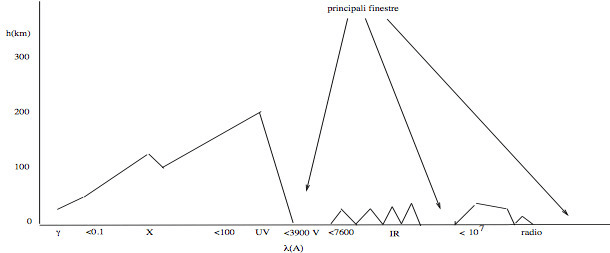
\includegraphics[width=(0.9\textwidth),height=(\textheight-11mm),keepaspectratio]{obswin}
\caption{Sopra la linea \'e possibile fare astronomia.}
\end{figure}

\begin{definition}{Luce visibile}
Visibile \numrange{3900}{7600}\si{\angstrom}
\end{definition}

\begin{definition}{Curve di sensibilit\'a del rivelatore $S(\lambda)$.}
\begin{itemize}
\item Curva visuale \numrange{5500}{6000}\si{\angstrom}
\item Curva fotografica \numrange{4000}{4500}\si{\angstrom}
\item Curva foto-visuale: riproduce il caso visuale tramite un filtro giallo e una lastra fotografica
\end{itemize}
\end{definition}

\begin{definition}{Larghezza banda (fotometria)}
\begin{itemize}
\item Banda larga: $>100\si{\angstrom}$.
\item Banda media: $\approx100\si{\angstrom}$.
\item Banda stretta: $<100\si{\angstrom}$
\end{itemize}
\end{definition}

\begin{figure}[!ht]
\centering
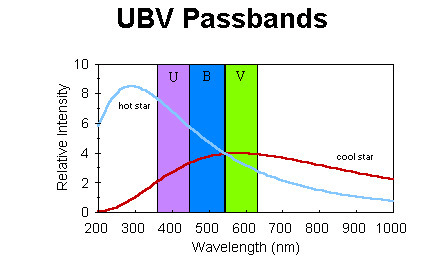
\includegraphics[width=(0.9\textwidth),height=(\textheight-11mm),keepaspectratio]{ubv}
\caption{Filtri passabanda UBV.}
\end{figure}

\clearpage



Sistemi che permettono osservazioni mediante filtri:
\begin{itemize}
\item Johnson-Morgan: (UBV) + 2 filtri VB (fotografici) e un terzo centrato sui \SI{3600}{\angstrom} in corrispondenza del salto di Balmer (FWHM:\SI{900}{\angstrom}, \SI{1000}{\angstrom}, \SI{700}{\angstrom}).
\item Ginevra: (UBV) + filtri nel visibile (a banda stretta)
\item Stromgren: 3 filtri UBV a banda stretta filtro Y intorno ai \SI{4700}{\angstrom} e un filtro centrato su linea idrogeno $H\beta$ ($2\to4$).
\item WUBV: band ($\lambda,\ \Delta\lambda$\si{\angstrom}) W($3270,\ 150$), U($3670,\ 260$), B($4295,\ 420$), V($5450,\ 850$)
\end{itemize}

Risposta di un Fotometro (visuale):
\begin{align*}
&f(\lambda)=S_VD_{\lambda}(\theta)A_{\lambda}f_{\lambda}\\
&I_V=\int_0^{\infty}f(\lambda)\,d\lambda\\
&=\int_0^{\infty}S_VD_{\lambda}(\theta)A_{\lambda}\lmono{}\frac{\,d\lambda}{4\pi r^2}
\end{align*}

Fatti:

\begin{itemize}
\item Wide band photometry: $B-V$. Limited by interstellar absorption.
\item Narrow band photometry: Strenght $H\gamma,\ H\delta$ to luminosity.
\item Ultraviolet method: Barbier-Chalonge, Balmer discontinuity at \mblock{\lambda=\SI{3647}{\angstrom}}.
\item Photographic method: ratio of absorption-line pairs.
\end{itemize}


\subsection{Magnitudine relativa}

In 1856, Norman Robert Pogson formalized the system by defining a first magnitude star as a star that is $100$ times as bright as a sixth-magnitude star, thereby establishing the logarithmic scale still in use today. This implies that a star of magnitude $m$ is $2.512$ times as bright as a star of magnitude $m+1$.

\subsubsection{Formula gi Pogson}

\begin{definition}{Magnitudine relativa}
\begin{equation*}
m_V=-2.5\log{I_V}+\const{}
\end{equation*}

Magnitudine di riferimento:
\begin{equation*}
-2.5\log{I_V*}+\const{}=0
\end{equation*}

\end{definition}

Vega ($\alpha$-Lyr)  ha magnitudine relative circa zero.

\subsection{Magnitudine assoluta}

Absolute magnitude is the measure of intrinsic brightness of a celestial object. It is the hypothetical apparent magnitude of an object at a standard distance of exactly \SI{10}{\parsec} (\SI{32.6}{\lightyear}) from the observer, assuming no astronomical extinction of starlight. This places the objects on a common basis and allows the true energy output of astronomical objects to be compared without the distortion introduced by distance. As with all astronomical magnitudes, the absolute magnitude can be specified for different wavelength intervals; for stars the most commonly quoted absolute magnitude is the absolute visual magnitude, which uses only the visual (V) band of the spectrum (UBV system). Also commonly used is the absolute bolometric magnitude, which is the total luminosity expressed in magnitude units that takes into account energy radiated at all wavelengths, whether visible or not.

\begin{definition}{Magnitudine assoluta}
\begin{equation*}
M_V=m_V+5\log{\frac{\SI{10}{\parsec}}{r}}-A
\end{equation*}
r \'e la distanza della stella (in pc), A rappresenta l'assorbimento interstellare (media di $\log{A_{\lambda}}$) dipende dalla distanza ed \'e massimo sul piano galattico ($\exv{A}\approx\frac{r}{2000\si{\parsec}}$).
\end{definition}

\begin{definition}{Magnitudine bolometrica.}
\'E la magnitudine che otterremmo raccogliendo tutta la luce che giunge all'orbita terrestre (\mblock{A_{\lambda}S_{\lambda}(\theta)=1}). Introduco la correzione bolometrica $BC$:
\begin{equation*}
m_{Bol}=m_V+BC
\end{equation*}
Scelgo che $BC\approx0$ per stelle che emettono nel visibile.
\end{definition}

Fatti:
\begin{itemize}
\item Allen (2000): $BC=0$ per supergiganti di classe di luminosit\'a 1 e tipo $F2$.
\end{itemize}

\begin{definition}{Magnitudine bolometrica assoluta.}
Magnitudine bolometrica assoluta:
\begin{align*}
&M_{Bol}=-2.5\log{\frac{L}{\lsun{}}}+4.74&\intertext{$4.74$ sarebbe la magnitudine bolometrica assoluta del sole se fosse a \SI{10}{\parsec}}\\
&(\lsun{}=\SI{3.845e33}{\erg\per\second})
\end{align*}
\end{definition}

\clearpage

\subsection{Indici di colore.}

\begin{definition}{Indicatori bande sistemi fotometrici}
Zona dello spettro: Lettera del filtro, Punto medio della radiazione effettiva  $\lambda_{eff}$
per il filtro standard, $FWHM$, Variante/i,	Descrizione.
\begin{itemize}

\item   Ultravioletto:
 U , $365 nm$ ,	$66 nm$ ,	$u, u', u*$,	"U" sta per "ultravioletto".
 
\item Visibile:

B, $445 nm$ , $94 nm$, $b$,	"B" sta per "blu".

V,	$551 nm$ , $88 nm$, $v, v'$, "V" sta per "visibile".

G, , , $g, g'$, "G" sta per "green" (verde).

R, $658 nm$, $138 nm$, $r, r', R', Rc, Re, Rj$, "R" sta per "rosso".

\item Infrarosso vicino:

I, $806 nm$, $149 nm$, $i, i', Ic, Ie, Ij$, "I" sta per "infrarosso".

Z ,,, z, z',.

Y $1020 nm$, $120 nm$, $y$,.

J, $1220 nm$, $213 nm$, $J', Js$,.

H, $1630 nm$, $307 nm$,,,.

K, $2190 nm$, $390 nm$, $K$, Continuum, K', Ks, Klong, K8, nbK.

L, $3450 nm$, $472 nm$, $L', nbL'$,.

\item Infrarosso medio:

M, $4750 nm$, $460 nm$, $M', nbM$,.	
N , , , $N1, N2, N3$,.

Q, , ,$ Q'$,.
 	
\end{itemize}     

\end{definition}

\begin{align*}
&U-B=m_U-m_B\\
&B-V=m_B-m_V&\intertext{Una stella blu ha $B-V$ pi\'u basso di una stella rossa.}
\end{align*}

Fissiamo le costanti per avere per stelle $A0$
\begin{equation*}
m_V\approx m_B\approx m_U
\end{equation*}
La distanza provoca uno spostamento verso il rosso: $E(B-V)\approx0.3 A$, $E(U-B)\approx0.1A$.

\subsection{SAAO Standards for Optical Photometry}

\begin{itemize}
    \item Harvard E-Region. 48 equal areas into which Pickering divided the sky
    \item $UBVR_cI_c$. optical UBV + R e I. The colour $(V-I)_C$ is a good temperature indicator that is less sensitive to gravity effects than $(B-V)$, $(U-B)$ is strongly affected by H Balmer absorption: together these 3 colors are usefull to determine color excess of stars (scattering/absorption of star light by interstellar dust).
    \item Str\"omgren $uvby$. Intermediate-band photometric system, narrower band. Metallicity index \mblock{m_1=(v-b)-(b-y)}. The index \mblock{c_1=(u-v)-(v-b)} is a mesure of Balmer discontinuity and thus a T index for OB stars and a surface gravity index for AF stars.
    \item $H\beta$. Intermediate pass-band (\mblock{FWHM\approx\SI{150}{\angstrom}}) and a narrow pass-band (\mblock{FWHM\approx\SI{30}{\angstrom}}) both centered on the Balmer $H\beta$ line of Hydrogen. A magnitude difference between the two filter measure the strength of $H\beta$: good surface gravity/luminosity index for OB stars and good T index for AF stars
    \item DDO. Intermediate pass-band filters (and narrow filter), $FWHM\approx\SI{80}{\angstrom}$. The system was intended for measure integrated light from galaxy nuclei to construct stellar population model for galaxies. The six pass-band are centered between \SIrange{3500}{4800}{\angstrom} and colours of the form $C(35-38)$, $C(38-41)$, \ldots are derived giving parameter related to Balmer discontinuity, line blanketing near \SI{4100}{\angstrom}, strength of CN absorption and G-band break. Usefull for F-K type stars.
\end{itemize}



\section{Stelle doppie.}

\begin{todo}{Stelle doppie}
Le stelle doppie: metodi di osservazione, problematiche generali; effetti di selezione. le stelle doppie per la stima delle masse e dei raggi delle stelle. relazioni massa-raggio e massa-luminosit\'a. 
\end{todo}


Circa la met\'a delle stelle osservate fanno parte di un sistem binario e in sistemi multipli si hanno spesso sottosistemi doppi poco influenzati dalle altre masse.

Dal moto orbitale posso ricavare in situazioni favorevoli
\begin{itemize}
    \item Somma delle masse
    \item Rapporto delle masse
    \item (Luminosit\'a delle componenti)
    \item Periodo orbitale
\end{itemize}


\subsection{Binarie visuali.}

Separazione angolare minore osservabile:

\SI{1}{\arcsec} dalla Terra, limitata dalle dimensioni del telescopio dallo spazio (circa \SI{e-2}{\arcsec}).

I sistemi pi\'u facilmente osservabili sono quelli a periodo lungo (grande separazione) e non troppo distanti:

un sistema a \SI{100}{\parsec} ha separazione \SI{1}{\arcsec} se \'e largo \SI{100}{\astronomicalunit} (per masse solari il periodo \'e di centinaia di anni).

Quindi le regole di selezione porteranno ad osservare con maggior frequenza sistemi vicini e di periodo lungo ma osservabile con stessa luminosit\'a delle componenti (sistemi gemelli).

Masse e raggi.

Terza legge di Keplero:
\begin{align*}
    &M_1+M_2=\frac{4\pi^2a^3}{GP^2}\\
    &M_1+M_2=\frac{1}{P^2}(\frac{a}{\Pi})^3&\intu{P in anni solari, a in arcsec, M's in $\msun{}$}
\end{align*}

quindi nota la parallasse $\Pi$, osservati $P$ e $a$ si ricava la somma delle masse.

Per ricavare le masse analizzo il moto delle due componenti rispetto al CM:

\subfile{tikz/binaryV}

\begin{equation*}
    \frac{M_1}{M_2}=\frac{a_2}{a_1}
\end{equation*}

\subsection{Binarie spettroscopiche.}

Misura la variazione periodi della velocit\'a radiale misurata tramite effetto Doppler.

Classi di oggetti privilegiati:
\begin{itemize}
    \item Oggetti non troppo deboli: spettro a media dispersione.
    \item Periodi non troppo lunghi: un periodo di $T\approx\SI{100}{\year}$ per masse solari comporta una $V_R\approx\SI{1}{\kilo\meter\per\second}$ (difficile da osservare), un periodo $T\approx\SI{1}{\year}$ comporta una $V_R\approx\SI{10}{\kilo\meter\per\second}$.
    \item A seconda del rapporto fra le luminosita sono osservabili una sola o entrambe le componenti.
\end{itemize}

Masse e raggi.
Sistema non risolto spazialmente, tengo conto dell'inclinazione del piano dell'orbita rispetto al piano notmale alla linea di vista moltiplicando ambo i membri della terza legge di Keplero per $\sin{i}$:

\begin{equation*}
    (M_1+M_2)\sin^3{i}=\frac{4\pi a^3\sin^3{i}}{GP^2}
\end{equation*}

Se sono note le velocit\'a radiali di ambo le componenti da \mblock{\frac{M_1}{M_2}=\frac{a_2\sin{i}}{a_1\sin{i}}=\frac{v_{2R}}{v_{1R}}} ottengo \mblock{M_1\sin^3{i}$ e $M_2\sin^3{i}}.

Se \'e nota solo una componente posso misurare
\begin{align*}
    &\frac{4\pi^2}{GP^2}a_1^3\sin^3{i}=(M_1+M_2)\sin^3{i}\frac{M_2^3}{(M_1+M_2)^3}&\intertext{quindi}\\
    &a=a_1+a_2=a_1(1+\frac{a_2}{a_1})=a_1(1+\frac{M_1}{M_2})\\
    &=a_1\frac{(M_2+M_1)}{M_2}
\end{align*}

Definisco la funzione di massa

\begin{equation*}
    f(M_1,M_2)=\frac{v_1^3P}{2\pi G}=\frac{(M_2\sin^3{i})^3}{(M_1+M_2)^2}
\end{equation*}

Fatti:
\begin{itemize}
    \item Se il sistema \'e anche fotometrico posso ricavare $\sin{i}$.
    \item Per $i=\frac{\pi}{2}$ ottengo un limite inferiore per le masse.
\end{itemize}

\subsection{Binarie a eclisse (fotometriche).}

Tecniche fotometriche: eclisse parziale/totale fra le componenti.

Osservabilit\'a dipende da inclinazione del piano dell'orbita rispetto alla linea di vista: l'angolo massimo dipende dalle dimensioni degli astri e dalla loro separazione.

Fatti:
\begin{itemize}
    \item Un periodo di un anno fra 2 stelle simili al Sole permette eclissi se l'angolo fra la linea di vista e il piano dell'orbita \'e minore di \ang{1;;}
    \item Separazione di pochi raggi stellari: per stelle non giganti periodo di giorni.
\end{itemize}

Masse e raggi.

\begin{figure}[!ht]
\centering
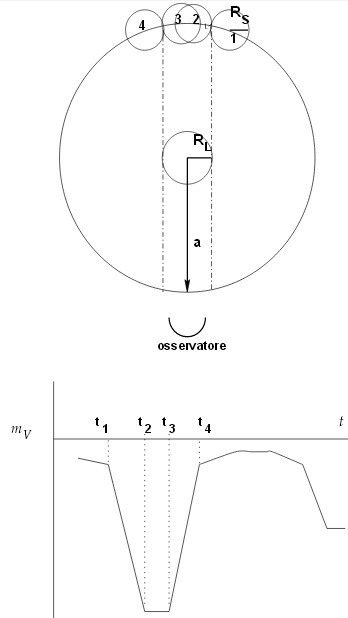
\includegraphics[width=\textwidth,height=0.9\textheight,keepaspectratio]{binaryE}
\caption{Binarie a eclisse.}\label{fig:binaryE}
\end{figure}

Analisi curva di luce (vedi \ref{fig:binaryE}):

\begin{align*}
    &M_1+M_2=\frac{4\pi^2a^2}{P^2G}&\intu{Terza legge di Keplero,}\\
    &\frac{t_4-t_1}{P}=\frac{2(R_L+R_S)}{2\pi a}\\
    &\frac{t_3-t_2}{P}=\frac{2(R_L-R_S)}{2\pi a}&\intertext{quindi ricavo $\frac{R_L}{a}$, $\frac{R_S}{a}$.}
\end{align*}

Ricavo le relazioni semi-empiriche per le stelle della MS \index{Relazioni semiempiriche MS.}:

\begin{align*}
    &R\propto M\expy{\frac{1}{2}}\\
    &L\propto \left\{\begin{array}{c}
         M^4,\ M<0.8\msun{}  \\
         M^3,\ M>0.8\msun{}  \\
    \end{array}\right.
\end{align*}

\clearpage


\chapter{Spettri stellari: Spettroscopia.}
\PartialToc

\section{Formazione spettri stellari: righe di assorbimento.}
Classificazione degli spettri stellari. Classi di luminosit\'a. 
Elementi di teoria delle righe spettrali. larghezza naturale di una riga. Introduzione ai fenomeni di allargamento. 
Allargamento delle righe spettrali: vari effetti. Spettri ad alta, media e bassa dispersione.

\subsection{Emission Line (Nebulae)}

Strong emission line owing to allowed/forbidden transitions of heavy elements (N, O, Ne, S, Cl, Ar, P, Fe, Ca, Mn, Cr, V, Co, Ni) in varous ionization stages: allowed transition are accounted for by electric dipole radiation, whereas forbidden transitions are due to magnetic dipole / electric quadrupole radiation. Forbidden emeission lines result from collisional excitation of metastable levels were first identified in gaseus nebula by Bowen (1928).


\subsubsection{Idrogeno}

\begin{definition}{Salto di Balmer}
Balmer jump or Balmer discontinuity is the difference of intensity of the stellar continuum spectrum on both sides of the limit of the Balmer series of hydrogen at \SI{364.6}{\nano\meter}. It is caused by electrons being completely ionized directly from the second energy level of a hydrogen atom (bound-free absorption), which creates a continuum absorption at wavelengths shorter than \SI{364.6}{\nano\meter}.

In some cases the Balmer discontinuity can show continuum emission, usually when the Balmer lines themselves are strongly in emission. Other hydrogen spectral series also show bound-free absorption and hence a continuum discontinuity, but the Balmer jump in the near UV has been the most observed.

The strength of the continuum absorption, and hence the size of the Balmer jump, depends on temperature and density in the region responsible for the absorption. At cooler stellar temperatures, the density most strongly affects the strength of the discontinuity and this can be used to classify stars on the basis of their surface gravity and hence luminosity. This effect is strongest in A class stars, but in hotter stars temperature has a much larger effect on the Balmer jump than surface gravity.
\end{definition}

\begin{definition}{Serie di Balmer}
\begin{figure}[!ht]
\centering
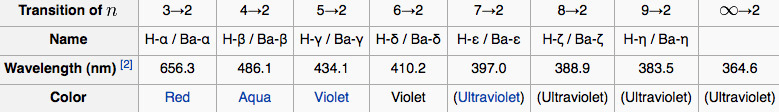
\includegraphics[width=(0.9\textwidth),height=(\textheight-11mm),keepaspectratio]{Bserie}
\caption{Serie di Balmer.}
\end{figure}
\end{definition}

\subsection{Atmosfera stellare}

Lo spettro di una stella \'e caratterizzato da una distribuzione simile a quella di un corpo nero per cui si pu\'o definire una lunghezza d'onda di massima emissione e da righe di assorbimento che danno informazioni sulla struttura chimico-fisica dell'atmosfera: lo spettro risulta dai fotoni provenienti dagli strati esterni dell'atmosfera fino ad una certa profondit\'a ottica e dal loro assorbimento negli strati attraversati.

\begin{usefull}{Radiative transfer equation}
\begin{align*}
&\mu\TDy{I_{\nu}}{\tau_{^nu}}=I_{\nu}-S_{\nu}&\intertext{$S_{\nu}$ is the source function ratio between emission and ambsorption coefficients, in thermodynamic equilibrium $B_{\nu}(T)$ is the source function:}\\
&j_{\nu}=\kappa_{\nu a}\frac{cu_{\nu}}{4\pi}=\kappa_{\nu a}B_{\nu}(T)\\
&d\tau_{^nu}=-\kappa_{nu}\rho\,dr\\
&\mu=\cos{\theta}\\
&I_{\nu}(0,\mu)=\frac{1}{\mu}\intzi{}S_{\nu}(\tau_{\nu})\exp{-\frac{\tau_{\nu}}{\mu}}\,d\tau_{\nu}
\end{align*}
\end{usefull}

\begin{usefull}{Thermodynamical equilibrium}
A single value T is sufficient to describe thermodynamic state everywhere: the particles have a maxwellian velocity distribution for that T, state of excitation and ionization for that T (according to Boltzmann/Saha equations) and radiation is homogeneous and isotropic, described by Kirchhoff-Plank function \mblock{B_{\nu}(T)=\frac{2h\nu^3}{c^2}\frac{1}{\exp{\frac{h\nu}{kT}}-1}}.
\end{usefull}

\begin{usefull}{Local thermodynamic equilibrium}
In LTE a single temperature suffice to describe properties of particles  at certain place and $S_{\nu}=B_{\nu}(T)$. The validity of LTE assumption depends on thermalization length, distance over which particle/photon emitted in a collision/transition has undergone sufficient collision/absorption-emission so that it cannot be distinguished within respective distribution.
\end{usefull}

\begin{usefull}{Eddington Approximation.}

\begin{equation*}
d\tau=-\kappa\rho\,dr
\end{equation*}

probabilit\'a che ha un fotone, prima di uscire dall'atmosfera, di essere assorbito: $\tau=0$ sulla superficie, $\tau=1$ \'e un libero cammino medio di profondit\'a.

\begin{align*}
&L=\intzi{}L(\tau)\exp{-\tau}\,d\tau&\intertext{$L(\tau)$ \'e la luce emessa dallo strato a profondit\'a ottica $\tau$.}
\end{align*}

Ammettiamo che l'emissione da uno strato dipenda solo da T il problema si riduce a ricavare $\tau(T)$: integrazione equazione del trasporto.

Nei modelli stellari si usano relazioni semi-empiriche $T(\tau,T_e)$:
\begin{align*}
&T^4=\alpha T_e^4P_n(\tau)&\intertext{$P_n(\tau)$ \'e un polinomio, $l(T)=aT^4$,}\\
&L\approx aT_e^4=4\pi R^2\sigma T_e^4
\end{align*}

\end{usefull}

Fatti:
\begin{itemize}
\item $T_e^{\odot}=\SI{5777}{\kelvin}$
\item L'andamento delle righe di assorbimento verso l'energia di legame del livello $n=2$ diminuisce il flusso in questa regione dello spettro.
\end{itemize}


\subsubsection{Intensit\'a di una riga.}

\begin{definition}{Larghezza equivalente $W_{\lambda}$}
La larghezza che avrebbe una riga corrispondente alla medesima sottrazione di energia con profilo rettangolare, completamente nera.
\begin{align*}
&W_{\lambda}=\int_{Riga}\,d\lambda(1-\frac{F(\lambda)}{F_{Cont}(\lambda)})&\intertext{$F(\lambda)$ \'e il flusso reale, $F_{Cont}(\lambda)$ \'e il flusso in assenza della riga.}
\end{align*}
\end{definition}

La larghezza equivalente \'e una misura dell'intensit\'a di una riga cio\'e del numero di particelle utili ad effettuare l'assorbimento (circa lineare con $W_{\lambda}$).


\subsection{Profilo e larhezza naturale di una riga.}

I'assorbimento di un fotone di energia $h\nu$ pu\'o causare una transizione fra due livelli atomici separati da energia del fotone. La sezione d'urto per atomo \'e della forma
\begin{equation*}
\sigma_{bb}=\frac{e^2}{4\epsilon_0m_ec}f\phi(\nu)
\end{equation*} fotoni assorbiti 

\begin{usefull}{Lorentzian and Gaussian profile}

\begin{align*}
&\phi_L\propto\frac{\gamma}{(\nu-\nu_0)^2+(\frac{\gamma}{4\pi})^2}\\
&\phi_C(\Delta\nu)=\frac{\gamma}{(2\pi\Delta\nu)^2+(\frac{\gamma}{4})^2}\\
&\phi_G\propto\frac{1}{\gamma}\exp{-(\frac{\nu-\nu_0}{\Delta\nu}}\\
&\phi_D(\Delta\nu_D)=\frac{1}{\sqrt{\pi}\Delta\nu_D}\exp{-(\frac{\Delta\nu}{\Delta\nu_D})^2}
\end{align*}

\begin{figure}[!ht]
\centering
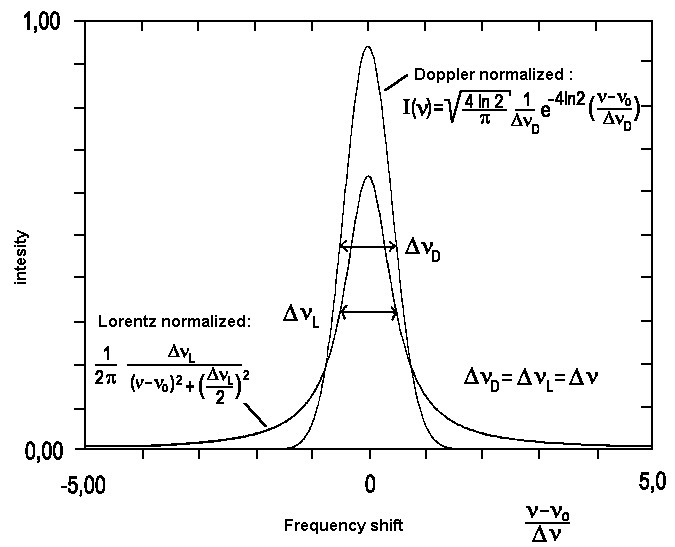
\includegraphics[width=(0.99\textwidth),height=(\textheight),keepaspectratio]{GLprofile}
\caption{Lorentzian vs Gaussian profile (in G manca un quadro all'esponente?!).}
\end{figure}


\end{usefull}

\clearpage

\subsubsection{Natural broadening (radiation damping)}

The motion of optical electron in a EM field of plane wave obey the (forced, damped) oscillation motion
\begin{equation*}
\ddot{x}+\gamma\dot{x}+\omega_0^2x=\frac{eE}{m}\cos{\omega t}
\end{equation*}

The oscillating (accelerating) charge radiate itself: the system losses energy.

Rate of energy radiation $P=\frac{2}{3}\frac{e^2\ddot{x}^2}{4\pi \epsilon_0c^3}$.

Classical absorption cross section
\begin{align*}
&a(\omega)=\frac{8\pi e^2}{3m_e^2c^4}[\frac{\omega^4}{(\omega^2-\omega_0^2)^2+\gamma^2\omega^2}]&\intertext{$\gamma$ is the classical damping constant}\\
&\gamma=(\frac{2e^2}{3m_ec^3})\omega_0^2
\end{align*}

Il principio di indeterminazione ci dice che un livello atomico non ha energia definita $E_i$ ma \'e una sovrapposizione di stati possibili attorno ad $E_i$: \mblock{\Delta \nu=\frac{\Delta E}{h}}. Transitions of electrons between levels doesn't correspond to specified energy difference.

Replace $\gamma$ with QM damping constant
\begin{align*}
&\Gamma_i=\sum_{l<i}A_{il}\\
&\Gamma_j=\sum_{l<j}A_{jl}
\end{align*}

\begin{definition}{Einstein coefficient $A_{ij}$}
The Einstein coefficient $A_{ij}$ is the probability in  unit of \si{\per\second} of a transition from upper level i to lower level j.
\end{definition}

The resulting profile for absorption cross section of a transition between two states reflects intrinsic energy width of both states: \mblock{\gamma_{nat}=\frac{\Delta E_i-\Delta E_f}{h/(2\pi)}}


\subsection{Absorption cross-section.}

Normalized absorption cross section for damping constant
\begin{align*}
&\phi_{\nu}=\frac{\frac{\Gamma}{4\pi^2}}{(\nu-\nu_0)^2+\frac{\Gamma^2}{(4\pi)^2}}\\
&\phi_{Max}=\phi_{\nu_0}=\frac{4}{\Gamma}\\
\end{align*}

For allowed transitions $\Delta\nu_{\frac{1}{2}}=\frac{\Gamma}{2\pi}\leq \SI{e-5}{\nano\meter}$ (FWHM), $\Delta\lambda=\frac{c}{\nu^2}\Delta\nu=\frac{2\pi}{3}\frac{e^2}{m_ec^2}\approx\SI{e-4}{\angstrom}$.

\subsection{Corpo nero}

L'energia irradiata per unit\'a di tempo per unit\'a di superficie nell'angolo solido $4\pi$ da un corpo nero di temperatura T
\begin{align*}
&(\int\,d\Omega I_{\nu}=)S_{\nu}=\frac{(4\pi)2 h\nu^3}{c^2}\frac{1}{\exp{\frac{h\nu}{KT}}-1}&\intu{nell'intervallo di frequenza $\nu,\nu+\,d\nu$, $\nu=\frac{c}{\lambda}$, $d\nu=-c\frac{d\lambda}{\lambda^2}$}\\
&(\int\,d\Omega I_{\lambda}=)S_{\lambda}=\frac{(4\pi)2 hc^2}{\lambda^5}\frac{1}{\exp{\frac{hc}{\lambda KT}}-1}&\intu{nell'intervallo di frequenza $\lambda,\lambda+\,d\lambda$}\\
&W=\sigma T^4&\intu{Legge di Stefan-Boltzmann}
\end{align*}

Il massimo di $S_{\lambda}$ segue la legge di Wien $\lambda_{Max}T=\const{}$.

\begin{definition}{Temperatura efficace}
\begin{equation*}
L=4\pi R^2\sigma T_e^4
\end{equation*}
\end{definition}

\begin{definition}{Temperatura di brillanza}
\begin{align*}
&I_{\nu}=B_{\nu}(T_b)\\
&L_{\lambda}=4\pi R^2\frac{2\pi hc^2}{\lambda^5}\frac{1}{\exp{\frac{hc}{\lambda KT_b}}-1}
\end{align*}
\end{definition}

Per il sole: $T_b(UV)\approx 5000\si{\kelvin}$, $T_b(V)\approx 6000\si{\kelvin}$

\begin{definition}{Temperatura di colore}
Temperature of a true blackbody is determined by intensity at two wavelength: match to shape of continous spectrum rather integrated power. 

\begin{equation*}
\frac{L_{\lambda_1}^O}{L_{\lambda_2}^O}=\frac{S_{\lambda_1}}{S_{\lambda_2}}
\end{equation*}

\end{definition}

\begin{definition}{Color index}
$B-V$ is defined by measurng luminisity with blue sensitive photographic plate (B) and with yellow-sensitive plate and yellow filter (V).
\end{definition}


\section{Righe dell'idrogeno.}

I livelli energetici dell'idrogeno sono \mblock{E_n=-\frac{\ER{}}{n^2},\ \ER{}\approx\SI{13.6}{\ev}}.

\begin{figure}[!ht]
\centering
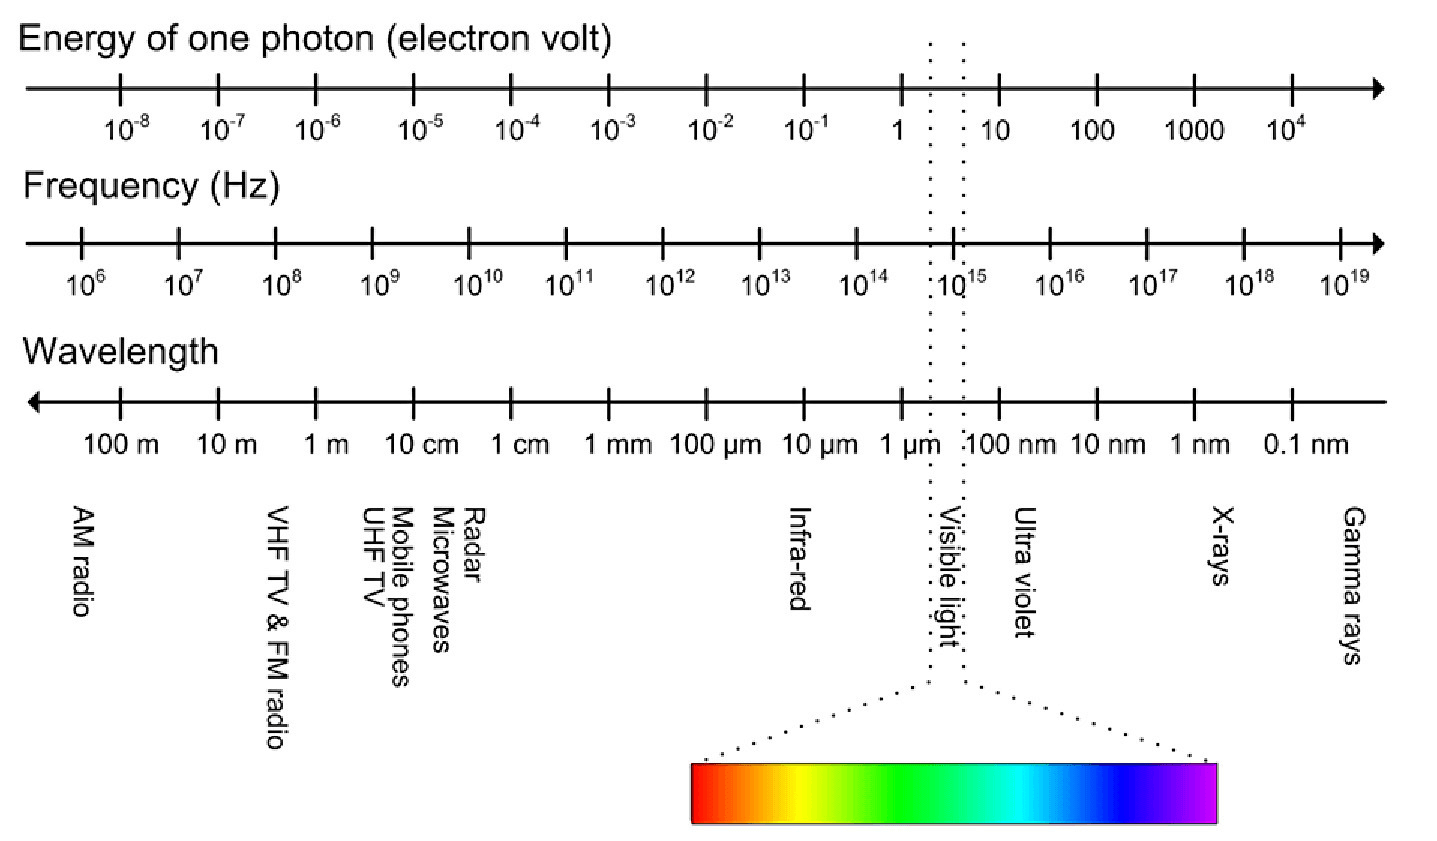
\includegraphics[width=(0.99\textwidth),height=(0.9\textheight),keepaspectratio]{PHevomega}
\caption{Spettro luminoso: energie, frequenze, regioni.}
\end{figure}

Le transizioni tra i livelli corrispondono a differenze di energie $E_{n,m}=\ER{}(\frac{1}{n^2}-\frac{1}{m^2})$
\begin{itemize}
    \item $n=1$: serie di Lyman (UV).
    \item $n=2$: serie di Balmer (V).
    \item $n=3$: serie di Paschen (IR).
\end{itemize}

\subsection{Popolazione dei livelli.}

A basse temperature H \'e neutro:
\begin{equation*}
    \frac{P(n)}{P(0)}\propto \exp{\frac{E_{0,n}}{KT}}
\end{equation*}
il rapporto \'e molto piccolo anche per $n=2$, primo eccitato.

A temperature intermedie (\SI{9520}{\kelvin}) la popolazione del primo eccitato $n=2$ raggiunge un massimo (stelle tipo spettrale A): le righe dell'idrogeno dominano lo spettro visibile.

\begin{figure}[!ht]
\centering
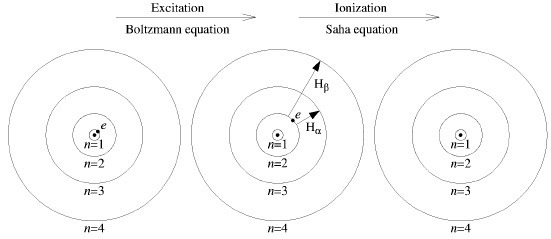
\includegraphics[width=(0.99\textwidth),height=(0.9\textheight),keepaspectratio]{boltzmansaha}
\caption{Determinazione popolazione livelli eccitati stati ionizzazione di H.}
\end{figure}

\begin{figure}[!ht]
\centering
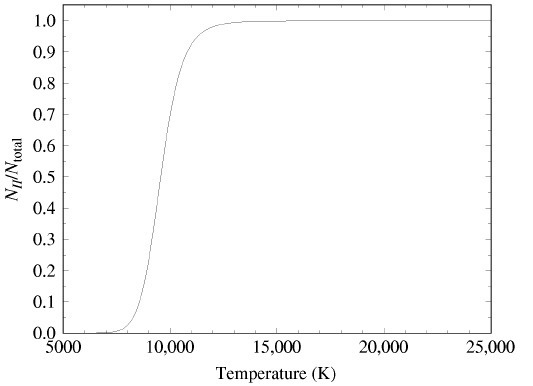
\includegraphics[width=(0.99\textwidth),height=(0.9\textheight),keepaspectratio]{HIIT}
\caption{Popolazione di HII.}
\end{figure}

\begin{figure}[!ht]
\centering
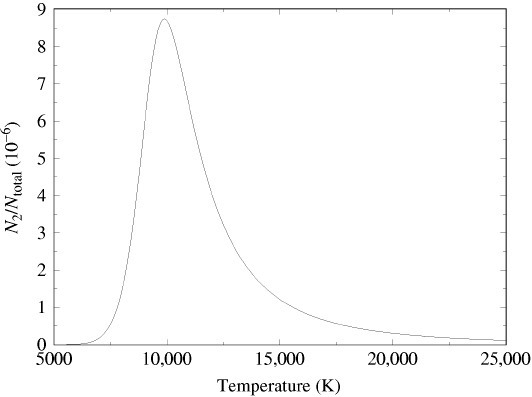
\includegraphics[width=(0.99\textwidth),height=(0.9\textheight),keepaspectratio]{HIn2pop}
\caption{Popolazione del livello primo eccitato di HI.}
\end{figure}

\clearpage

\section{Allargamento delle righe spettrali.}

\subsection{Allargamento (thermal) Doppler (GP)}

Lungo la linea di vista gli atomi hanno una distribuzione di velocit\'a gaussiana (moti termici e turbolenti)
\begin{align*}
&dn(v_e)\propto\exp{-\frac{v_e^2}{\alpha}}\,dv_e\\
&\alpha=\frac{2KT}{m}+v_{turb}^2
\end{align*}

La riga corrisponde ad una lunghezza d'onda diversa con
\begin{equation*}
\Delta\lambda\approx\frac{v_e}{c}\lambda
\end{equation*}

Per l'insieme degli atomi avremo una distribuzione di frequenze proprie

\begin{equation*}
\sigma(\nu)\propto\int\,d\nu*\exp{-A(\nu*-\nu_0)^2}\frac{1}{(\nu-\nu*)^2+(\frac{\gamma}{4\pi})^2}
\end{equation*}

Il profilo della riga \'e caratterizzato dalla curva pi\'u larga: Lorenziana, parametrizzata dalla larhezza naturale o gaussiana dalla distribuzione di velocit\'a.

Fatti:
\begin{itemize}
    \item Per il sole la gaussiana \'e pi\'u larga della lorenziana di un fattore \num{e3}.
\end{itemize}


\subsection{Allargamento da pressione (LP)}

La vicinanza di altre particelle perturba i livelli atomici (atmosfere con alta pressione): la condizione di equilibrio idrostatico in termini di profondit\'a ottica $\TDy{\tau}{P}=\frac{g}{\kappa}$ dice che nella regione $\tau\approx1$ la pressione $P_{Atm}\approx\frac{g}{\kappa}$, dove g \'e l'accelerazione di gravit\'a che determina l'allargamento da pressione mentre l'opacit\'a $\kappa$ varia meno rispetto a g.

Fatti:
\begin{itemize}
    \item La dominanza dell'allargamento da pressione nelle stelle di sequenza (nane) permette la classificazione empirica in classi di luminosit\'a.
\end{itemize}


\subsection{Allargamento quasi-statico.}

Effetto del campo esterno sull'atomo: perturba i livelli e cambia le energie di transizione. Distribuzione statistica nello spazio-tempo: distribuzione delle energie.

\mblock{\Delta t_{int}>\Delta T_{em}\approx\SI{e-9}{\second}}: nearby particles shift energy levels of emitting particle.

La larghezza \'e funzione soprattutto di $\rho$ (meno di $T$): si ha una dipendenza del tipo \mblock{\gamma\propto\exv{r}\expy{-n}}, con
\begin{itemize}
    \item Stark effect (WD): $n=3$.
    \item Van der Waals force (cool stars): $n=6$.
    \item Dipolar coupling between particles of same species: $n=3$.
\end{itemize}

\subsection{Allargamento da impatto (LP)}

Da un punto di vista semi-classico durante una collisione si interrompe l'assorbimento alla frequenza di transizione dell'atomo.

\mblock{\Delta t_{col}<\Delta T_{em}\approx\SI{e-9}{\second}}, funzione di $(T,\rho)$

\subsection{Allargamento dovuto alla rotazione.}

Ho un effetto Doppler di segno opposto nell zone simmetriche rispetto all'asse della superficie
\begin{equation*}
    \frac{\Delta\lambda}{\lambda}\approx\frac{\Delta v}{c}\approx2\frac{\omega R}{c}
\end{equation*}

Fatti:
\begin{itemize}
    \item Stelle rapidamente rotanti (A,O,B).
    \mblock{\omega R\approx v_F=\sqrt{\frac{2GM}{R}}\approx\SI{e3}{\kilo\meter\per\second}} e \mblock{\frac{\Delta\lambda}{\lambda}\approx\num{e-3}}: nel visibile $\Delta\lambda\approx\SI{10}{\angstrom}$.
    \item Le classi O,B sono rotatori veloci, il tipo A comprende rotatori lenti e veloci e $Ap$, i tipi spettrali pi\'u freddi da F in poi sono rotatori lenti.
\end{itemize}


\section{Astro-spettroscopia.}

\subsubsection{Spectral resolution.}

A varie dispersioni sul ricevitore gli spettri ci danno informazioni diversi
\begin{itemize}
    \item Bassa dispersione: \SI{e2}{\angstrom\per\milli\meter}.
    
    Tipo spettrale.
    
    \item Media dispersione: \numrange{10}{100}\si{\angstrom\per\milli\meter}.
        
    Velocit\'a radiale, allargamento righe: P,T, righe peculiari.
        
    \item Alta dispersione: $\leq$\SI{10}{\angstrom\per\milli\meter}.
    
    $W_{\lambda}(\eta_{\lambda})$: analisi quantitativa,  ricostruzione dell'atmosfera.

\end{itemize}


\subsubsection{Moto radiale.}

Le righe sono spostate verso il rosso/blu
\begin{align*}
    &\frac{\Delta\lambda}{\lambda}=z\approx\frac{v}{c}&\intu{small $v$}\\
    &1+z=\gamma(1+\frac{v_{\parallel}}{c})\\
    &v_{los}=c\exv{\frac{\Delta\lambda}{\lambda}}_{Righe}
\end{align*}

Classi di osservazioni:
\begin{itemize}
    \item Binarie spettroscopiche
    \item Stelle pulsanti
    \item Legge di Hubble: $v_{rad}\approx c$
\end{itemize}

\subsection{Gravitational red-shift}

Per oggetti densi \'e osservabile uno spastamento Doppler delle righe di assorbimento dovuto alla differenza tra energia gravitazionale sulla superficie della stella ed energia al punto d'osservazione:
\begin{align*}
&V_{grav}=\frac{GM}{Rc}\\
&\frac{\Delta\lambda}{\lambda}=\frac{E}{\Delta E}\overset{?}{=}\frac{Rc^2}{GM}
\end{align*}

\section{Classificazione degli spettri stellari}

In un grafico $U-B$ vs $B-V$ una successione di corpi neri di temperatura variabile \'e approssimativamente una linea retta.

\begin{figure}[!ht]
\centering
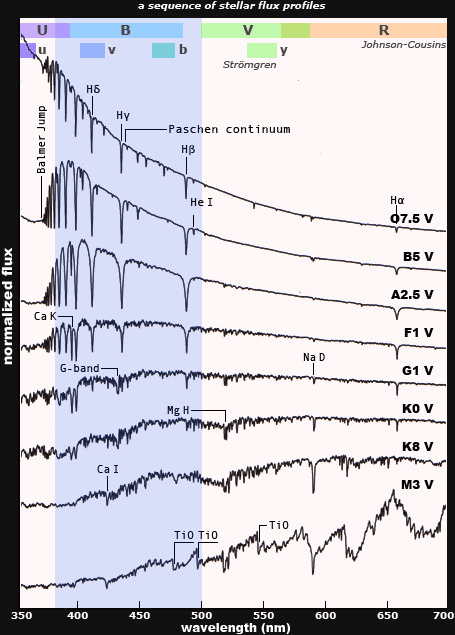
\includegraphics[width=(0.99\textwidth),height=0.9\textheight,keepaspectratio]{sequenceFP}
\caption{Sequence stellar flux profile.}
\end{figure}

La classificazione stellare consiste di una lettera per il tipo, numero per il sottotipo e un numero romano per la classe di luminosit\'a (I supergiganti, III giganti, IV subgiganti, V nane). Il tipo spettrale \'e individuato dalla distribuzione del continuo e dalla presenza di alcune righe.

La classe di luminosit\'a \'e individuata dalle caratteristiche delle righe: Larghezza/pressione supericiale.

\begin{figure}[!ht]
\centering
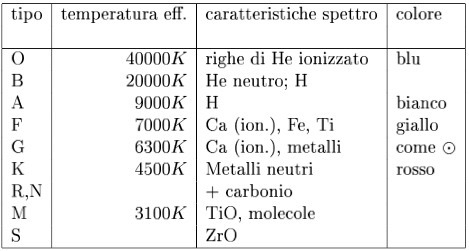
\includegraphics[width=(0.8\textwidth),height=(\textheight-11mm),keepaspectratio]{types}
\caption{Star types.}
\end{figure}

Fatti:
\begin{itemize}
\item O stars (\SI{30000}{\kelvin}): hottest stars, continuum strong in UV.

Strong He II lines in absorption, sometimes with few lines; He II dominates emission; He I lines weak but increasing in strength
from O5 to O9; hydrogen Balmer lines prominent but
weak relative to later types; lines of Si IV, O III, NIII
and C IV.

\item B stars (\SI{20000}{\kelvin}).

He I lines dominate, with maximum strength at B2; He I dominates He II lines virtually absent; hydrogen lines strengthening
from B0 to B9; Mg II and Si II lines

\item A stars (\SI{10000}{\kelvin}). 

Hydrogen lines reach maximum strength at A0; hydrogen Balmer lines dominate of ionised metals (Fe II, Si II, Mg II) at maximum strength near A5; Ca II lines strengthening; lines of neutral
metals appearing weakly.

\item F stars (\SI{7000}{\kelvin}).

Hydrogen lines weakening rapidly while H and K lines of CaII strengthen; neutral metal (Fe I and Cr I) lines gaining on ionised metal lines by large F

\item G stars (\SI{6000}{\kelvin}).

Hydrogen lines very weak; Ca II H and K lines reach maximum strength near G2; neutral metal (Fe I, Mn I,Ca I) lines strengthening while ionised metal lines
diminish; molecular G band of CH becomes strong.

\item Il sole \'e una stella di tipo G2.

\item K stars (\SI{4000}{\kelvin}).

Hydrogen lines almost gone; Ca lines strong; neutral metal lines very prominent; molecular bands of TiO begin (K2)
to appear by late K.

\item M stars (\SI{3000}{\kelvin}).

Neutral metal lines very strong; molecular bands prominent with TiO bands dominating by M5; vanadium oxide bands appear.

\end{itemize}


\begin{figure}[!ht]
\centering
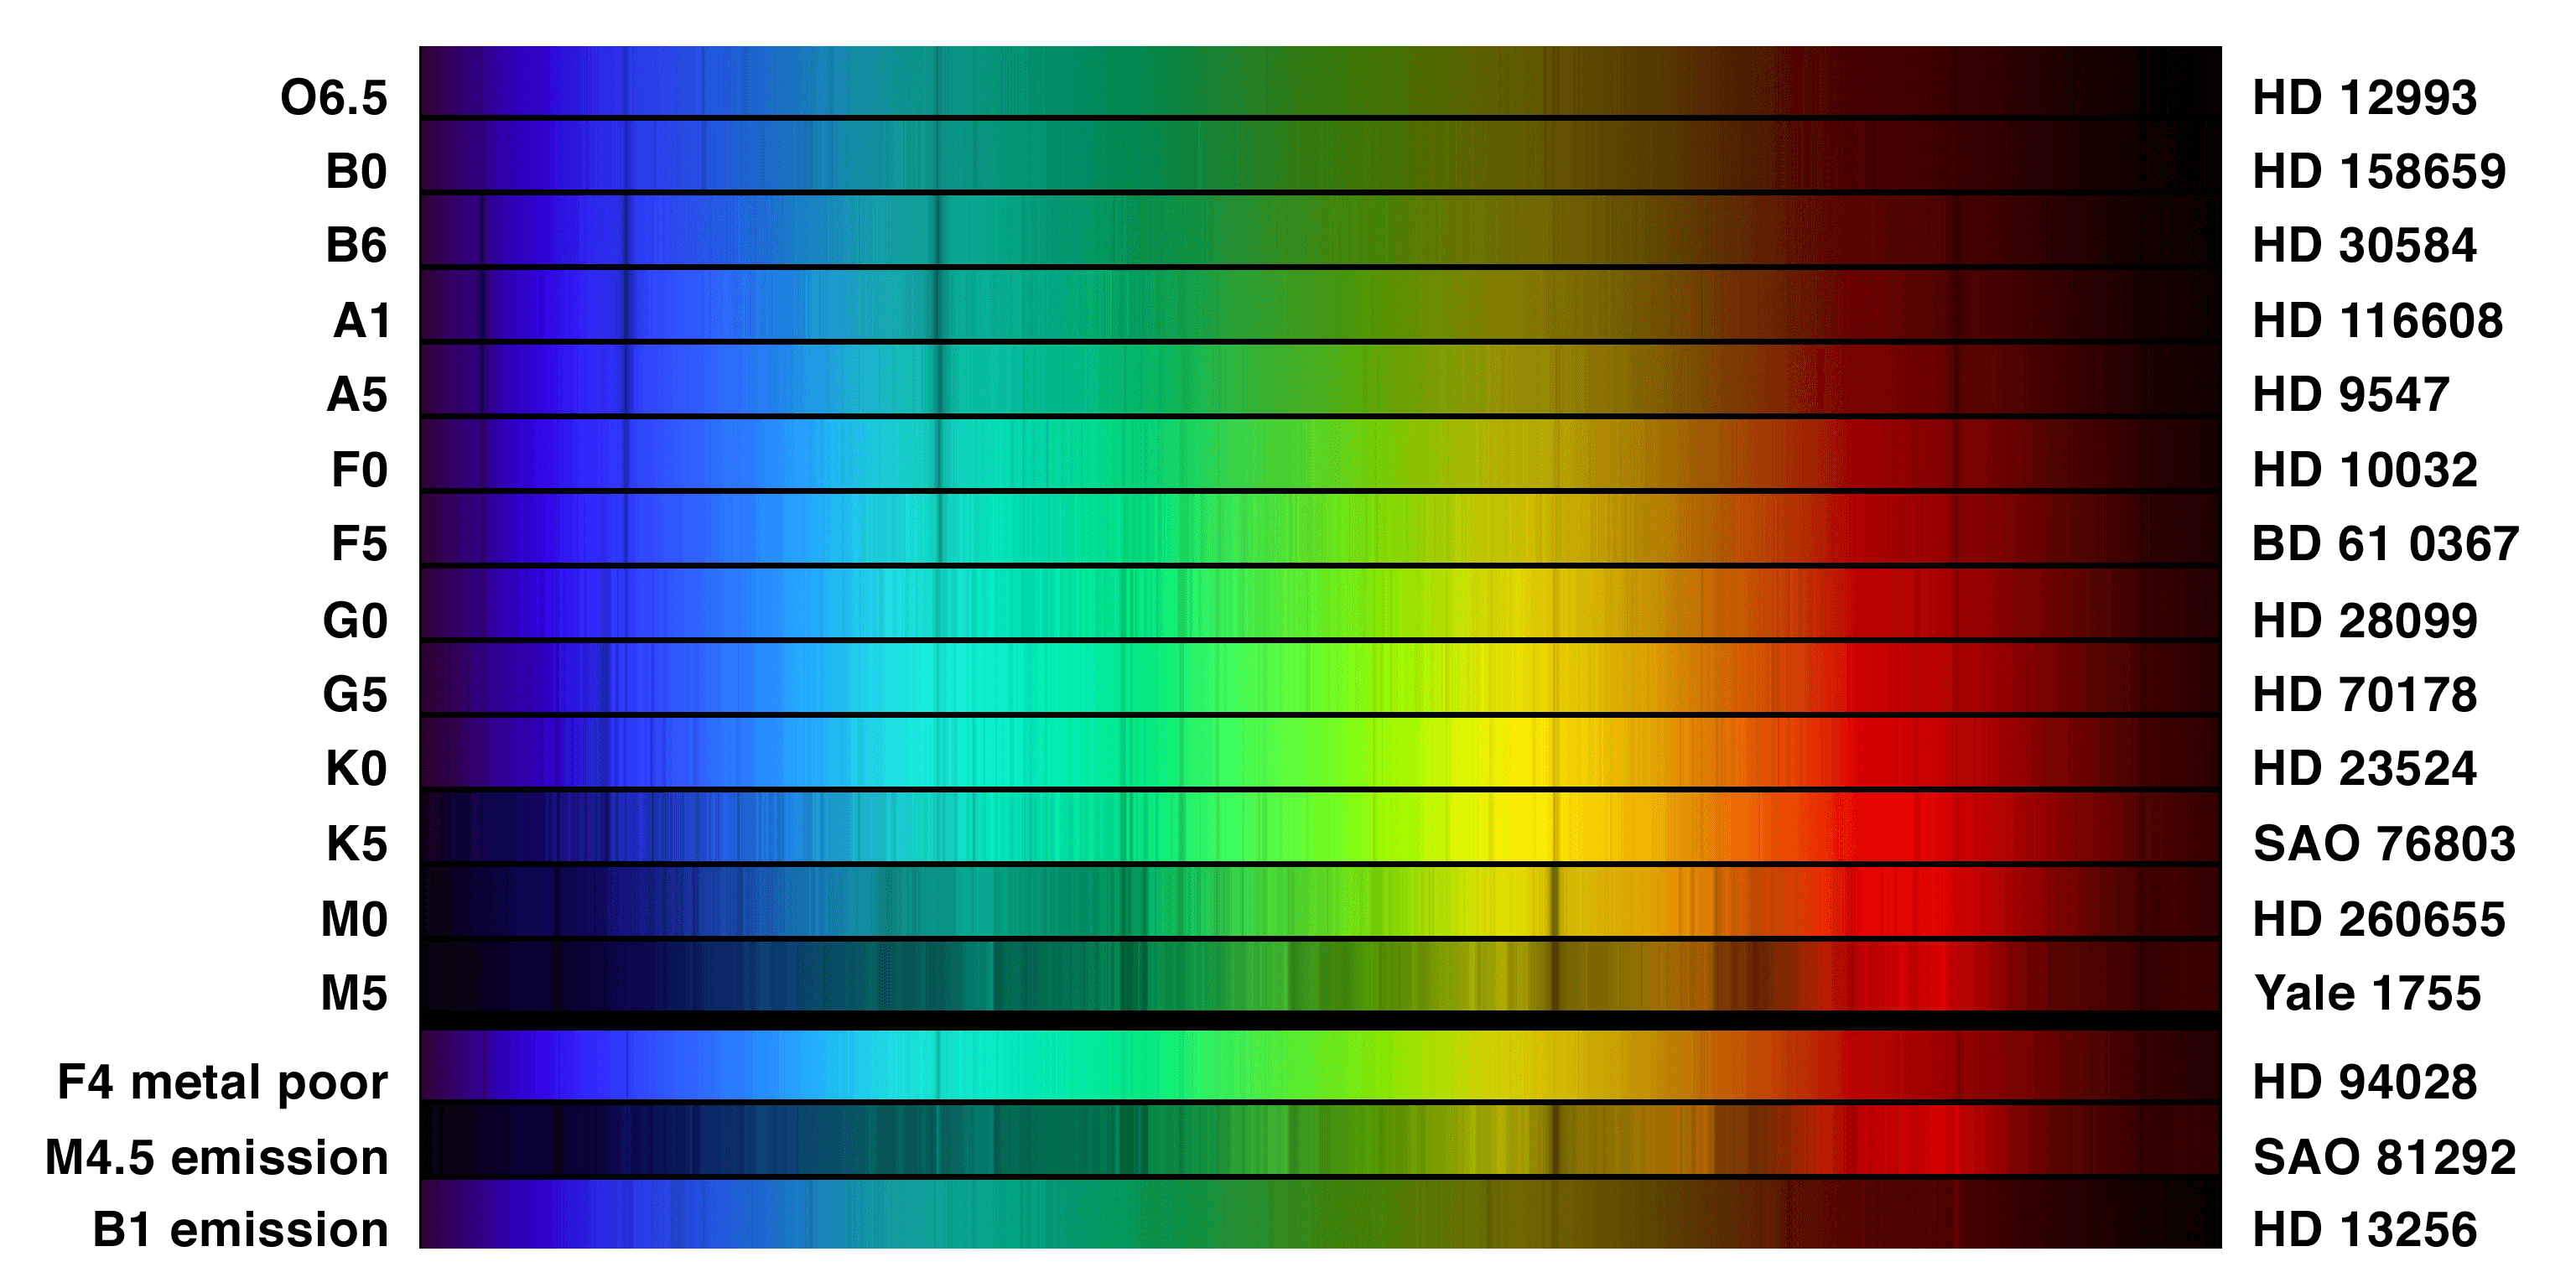
\includegraphics[width=(0.99\textwidth),height=\textheight,keepaspectratio]{spectral}
\caption{Spectral types.}
\end{figure}

\begin{figure}[!ht]
\centering
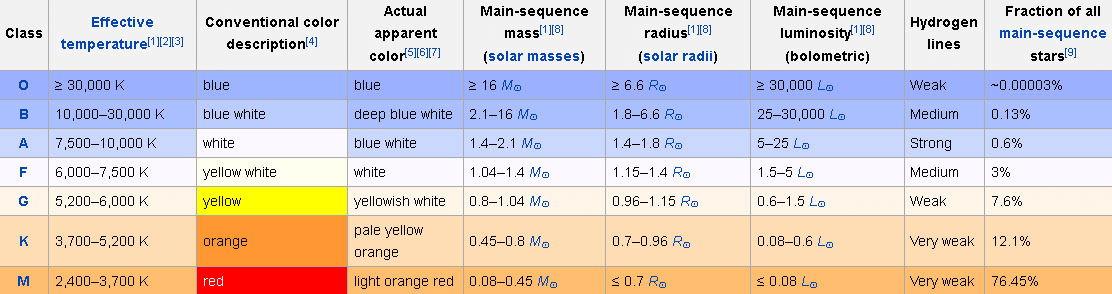
\includegraphics[width=(\textwidth),height=(\textheight-11mm),keepaspectratio]{classprop}
\caption{Classi stellari.}
\end{figure}

\clearpage



\chapter{Relazioni massa/luminosit\'a. Diagramma di \hr{}.}
\PartialToc

\subsection{Massa-Luminosit\'a}

\begin{usefull}{Massa-Luminosit\'a (relazione).}
\begin{align*}
    &\frac{L}{\lsun{}}\approx0.23(\frac{M}{\msun{}})\expy{2.3},\ (M<0.43\msun{})\\
    &\frac{L}{\lsun{}}\approx(\frac{M}{\msun{}})^4,\ (0.43\msun{}<M<2\msun{})\\
    &\frac{L}{\lsun{}}\approx1.5(\frac{M}{\msun{}})\expy{3.5},\ (2\msun<m<20\msun{})\\
    &\frac{L}{\lsun{}}\approx3200\frac{M}{\msun{}},\ (m>20\msun{})
\end{align*}
\end{usefull}



\section{Importanti relazioni semi-empiriche.}

\subsection{Massa-Luminosit\'a}

\begin{equation*}
    (\frac{L}{\lsun{}})=(\frac{M}{\msun{}})\expy{\frac{1}{4}}
\end{equation*}

\begin{todo}{Importanti relazioni semi-empiriche.}
clay pg 470-472.
$\S 1.6$ stellar interior
\end{todo}

\section{Diagrammi di HR: magnitudine vs colore.}


Considero il diagramma $M_V$ vs $(B-V)$ o $M_{B}$ vs spectral type (per stelle vicine) (\mblock{M_B=-2.5\log{\frac{L}{\lsun{}}}+4.72})

\subsection{Diagramma di HR per stelle vicine.}

\begin{figure}[!ht]
\centering
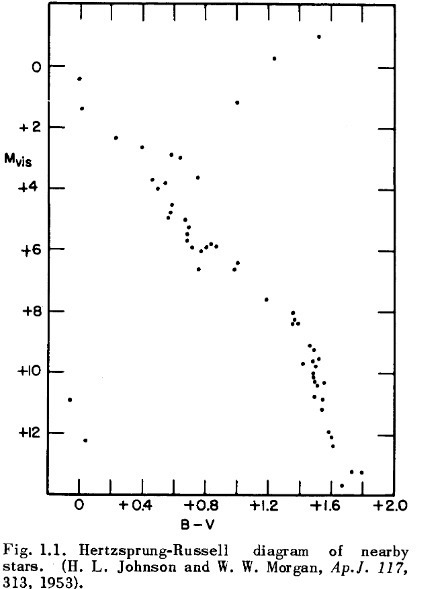
\includegraphics[width=(\textwidth),height=(0.8\textheight),keepaspectratio]{nearbyHR}
\caption{Diagramma HR di stelle vicine.}
\end{figure}

\clearpage

\subsection{Diagramma di HR per associazioni di stelle.}

Considero il diagramma di HR per associazioni fisiche di stelle.


La struttura di una stella \'e univocamente definita da massa, composizione chimica iniziale ed et\'a: un diagramma di ammasso si pu\'o vedere come una sequenza di stelle con massa variabile e stessa composizione iniziale ed et\'a.

\begin{figure}[!ht]
\centering
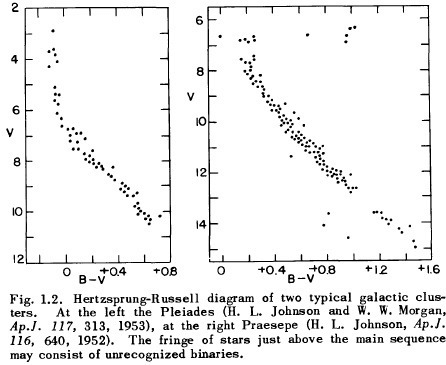
\includegraphics[width=(\textwidth),height=(\textheight-11mm),keepaspectratio]{GCHR}
\caption{Diagramma di HR di un cluster.}
\end{figure}


\begin{figure}[!ht]
\centering
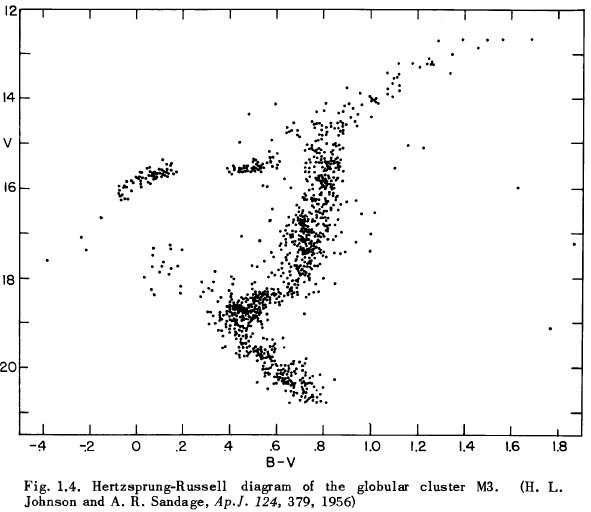
\includegraphics[width=(\textwidth),height=(\textheight-11mm),keepaspectratio]{GlobularCHR}
\caption{Diagramma di HR di un ammasso globulare.}
\end{figure}

\clearpage

\subsection{Evolution of a cluster of stars.}

\subsubsection{Evolution from main sequence.}

Il processo di fusione $4H\to He$ produce \SI{6.4e18}{\erg\per\gram}.

Suppongo che una stella di massa M si allontani dalla sequenza principale quando ha costituito un core di He di massa $fM$:

se $X_H$ \'e la frazione di H in massa originaria si deve convertire in He una massa $fX_HM$ di H quindi l'energia irradiata \'e $E=fX_HM(\num{6.4e18})=\num{1.3e52}fX_H\frac{M}{\msun{}}\si{\erg}$.

La vita di sequenza principale pu\'o essere stimata
\begin{equation*}
    \tau_E=\frac{E}{L}=\num{1.1e11}fX_H\frac{M/\msun{}}{L/\lsun{}}\si{\year}
\end{equation*}

Fatti:
\begin{itemize}
    \item Per stella solar-like $f=15\%$: using M/L relatioship
    \begin{equation*}
    \tau_E=\num{12e9}(\frac{L}{\lsun{}})\expy{-\frac{3}{4}}\si{\year}
    \end{equation*}
    \item Posso approssimare l'et\'a di un ammasso con l'et\'a delle sue stelle pi\'u luminose. 
\end{itemize}

Ad alta luminosit\'a la linea della sequenza principale svolta a destra.

\subsubsection{Turn-off: ramo delle giganti.}

Una classificazione dei diagrammi in sequenze di $(B-V)_{\text{Turn-off}}$ crescenti corrisponde ad una sequenza di et\'a: turn-off blue per ammasso giovane, turn-off giallo ammasso vecchio.


\begin{figure}[!ht]
\centering
\includegraphics[width=(\textwidth),height=(0.9\textheight),keepaspectratio]{extremeGCHR}
\caption{Diagramma di HR di cluster giovane (in alto) vecchio (in basso).}
\end{figure}

\clearpage

\section{Caratteristiche delle stelle nelle zone del diagramma di HR.}

\begin{figure}[!ht]
\centering
\includegraphics[width=(\textwidth),height=(0.9\textheight),keepaspectratio]{HRpizza}
\caption{Diagramma di HR: MS, WD, SD, giant branch.}
\end{figure}

\subsection{Passaggio al diagramma raggio-Luminosit\'a.}

Passo alla rappresentazione con in ordinata L e in ascissa $T_e$:

\begin{align*}
    &\log{\frac{L}{\lsun{}}}=\frac{1}{2.5}(M_{B\odot}-M_B)\\
    &=4\log{\frac{T_e}{T_{e\odot}}}+2\log{\frac{R}{\rsun}}
\end{align*}

\begin{figure}[!ht]
\centering
\includegraphics[width=(\textwidth),height=(\textheight-11mm),keepaspectratio]{CsHR}
\caption{Diagramma HR $L$ vs $T_e$.}
\end{figure}

\clearpage

\subsection{Nane.}



\subsection{Sub-nane.}

Caratteristiche:
\begin{itemize}
    \item Deboli righe di assorbimento.
    \item Parallela alla MS circa 1 magnitudine superiore.
    \item Per pari $T_e$ $\log{\frac{L_{SN}}{L_{MS}}}=-0.4$.
\end{itemize}

Le differenze di luminosit\'a e di caratteristiche spettrali sono attribuibili alla diversa composizione chimica.

Fatti:
\begin{itemize}
    \item La sequenza principale degli ammassi globulari coincide con quella delle sub-nane.
\end{itemize}

\subsection{Nane bianche.}

Caratteristiche:
\begin{itemize}
    \item Alta densit\'a superficiale: righe allargate.
    \item Raggio quasi costante circa $\frac{1}{100}\rsun{}$.
    \item Oggetti estremamente densi.
    \item Fase finale evoluzione stellare.
\end{itemize}


\section{Popolazioni stellari.}

Fatti:
\begin{itemize}
\item Existence in late F early G stars of strong-line and weak-line with different kinematical properties: generally the strong lines have low velocity, the weak line higher velocity.
\end{itemize}

\begin{figure}[!ht]
\centering
\includegraphics[width=(\textwidth),height=(\textheight-11mm),keepaspectratio]{Starpop}
\caption{Popolazioni stellari: distribuzione galattica.}
\end{figure}

\begin{figure}[!ht]
\centering
\includegraphics[width=(\textwidth),height=(\textheight-11mm),keepaspectratio]{starpops}
\caption{Popolazioni stellari: differenze orbitali.}
\end{figure}

\subsection{Cluster di stelle.}

\begin{definition}{Star cluster.}
Is a group of stars that have a much stronger gravitational attraction to each others than to general field of stars.
\end{definition}

\subsubsection{Globular cluster.}



\begin{itemize}
    \item Number of stars: approx. \num{e5}.
    \item Far from the Sun: magnitude of RR Lyra stars.
    \item Location: Corona or galactic nucleus.
    \item Diameter of high density region approx \SI{10}{\parsec}, density \SI{e3}{\per\parsec}.
    \item Diameter \numrange{50}{100} \si{\parsec}.
    \item Color of the brightest: red.
    \item Densit\'a di stelle (\si{\cubic\parsec}): \numrange{0.5}{e3}.
    \item Nomi: M3
\end{itemize}

\subsubsection{ Open Cluster (Galactic cluster).}

\begin{itemize}
    \item Few-thousands stars randomly distributed.
    \item Found in galactic disc.
    \item Location: disk.
    \item Number of stars: \numrange{50}{e3}.
    \item Color of the brightest: red/blue.
      \item Densit\'a di stelle (\si{\cubic\parsec}): \numrange{0.1}{10}.
    \item Nomi: Hyades, Pleiades.
\end{itemize}

\subsubsection{Association.}

Open cluster containing most luminous main sequence stars of type $O/B$. O stars are not randomly distributed: O/B/WR are scattered in a region of \SI{100}{\parsec}.

\begin{itemize}
    \item Location: spiral harms.
    \item Diameter: \numrange{30}{200}\si{\parsec}
    \item Number of stars \numrange{10}{100}?
    \item Color of the brightest: blue.
      \item Densit\'a di stelle (\si{\cubic\parsec}): \num{0.01}.
    \item Nomi: Orion.
\end{itemize}
    


Fatti:
\begin{itemize}
    \item Le supergiganti blu sono stelle giovani vicine a nubi interstellari.
    \item Espansione di ammassi/associazioni contenenti SG blue permette, ricostruendo all'indietro il loro moto, di limitare superiormente la loro et\'a a \SI{e8}{\year}.
    \item Le galassie ellittiche e gli ammassi globulari appaiono prive di gas interstellare e polvere (Highly stable dynamical system).
\end{itemize}


\subsection{Comportamento cinematico}

\'E possibile separare le stelle vicine in due gruppi:
\begin{itemize}
    \item Alta velocit\'a sul piano galattico.
    
    Giganti rosse (HR simile agli ammassi globulari), subnane, 
    
    \item Bassa velocit\'a sul piano galattico.
    
    Stelle di tipo O/B (HR simile ad ammassi galattici), nubi interstellari.
\end{itemize}

Fatti:
\begin{itemize}
    \item Gli ammassi galattici presentano moto d'insieme di moderata velocit\'a a differenza degli ammassi globulari.
    \item Ad alta velocit\'a sul piano galattico corrisponde alta velocit\'a ortogonale: configurazione sempre pi\'u sferica.
    \item Le stelle ad alta veloci\'a hanno un moto retrogrado sul piano galattico (alone esterno).
\end{itemize}

\subsection{Evoluzione della galassia.}

Trasformazione di una struttura quasi-sferica ad un disco accompagnato da un rarefatto alone.

\begin{todo}{High/low velocity galactic plane}
Moto retrogrado
\end{todo}


\subsubsection{Popolazione I.}

Si distinguono spettroscopicamente stelle con righe forti (lente) e stelle con righe deboli (veloci).

\begin{itemize}
    \item (Young) extreme pop I.
    
    Typical member: Blue giant, variabili T Tauri, Cefeidi.
    
    Where: ammassi aperti, galactic cluster, braccia a spirale, G (spirale, irregolare).
    
    AVG velocity: \SI{8}{\kilo\meter\per\second}. Shape of subsystem: flat. Distanza dal PG: \SI{60}{\parsec}.
    
    Metallicit\'a: $\frac{Z}{Z_{\odot}}>1$.
    
    Et\'a (risp. universo): \numrange{0}{0.005}.
    
    \item (Int.) Pop I. 
    
    Typical member: Stelle a forti righe metalliche, Supernovae II, vicine del Sole.
    
    AVG velocity: \SI{10}{\kilo\meter\per\second}.
    
    Distanza dal piano galattico: \SI{160}{\parsec}.
    
    Metallicit\'a: $\frac{Z}{Z_{\odot}}>0.75$.
    
    Et\'a (risp. universo): \numrange{0.05}{0.25}.
    
    Where: Disco.
    
    \item (Old/disc) Pop I. 
    
    Typical member: Stelle a deboli righe metalliche, novae,nebulase planetarie, RR Lyrae, Periodic ($P<0^d.4$).
    
    AVG velocity: \SI{16}{\kilo\meter\per\second}. Distanza dal piano galattico: \SI{300}{\parsec}.
    
    Metallicit\'a: $\frac{Z}{Z_{\odot}}>0.5$.
    
    Et\'a (risp. universo): \numrange{0.25}{0.8}.
    
    Where: Disco, nucleo galattico (Bulges).

\end{itemize}

\subsubsection{Popolazione II.}

Si distinguono ammassi globulari e stelle ad alta velocit\'a.

\begin{itemize}
    \item Intermediate Pop. II:
    
    Stelle: Stelle ad alta velocit\'a, variabili a lungo periodo, RR Lyrae.
    
    AVG velocity(ortogonale al piano galattico): \SI{25}{\kilo\meter\per\second}.
    
    Where: Galassie ellittiche, disco spesso, ammasso globulare.
    
    Distanza dal piano galattico: \SI{500}{\parsec}.
    
    Metallicit\'a: $\frac{Z}{Z_{\odot}}=0.25$.

    Et\'a in et\'a dell'universo: \numrange{0.8}{1}.

    \item Pop II di Bulge:
    
    Where: Nucleo galattico.
    
    Stelle: Nebulose planetarie, Cefeidi.
    
    Metallicit\'a: $\frac{Z}{Z_{\odot}}=\numrange{0.1}{2.}$.
    
    Et\'a in et\'a dell'universo: \numrange{0.5}{1}.
    
    \item Extreme (halo) Pop. II:
    
    Stelle: Bright red giants, globular cluster, subdwarf, RR Lyrae $\Pi>0^d.4$, ramo orizzontale HR.
    
    AVG velocity(ortogonale al piano galattico): \SI{75}{\kilo\meter\per\second}.
    
    Where: Ammassi globulari, galassie ellittiche.
    
    Distanza dal piano galattico: \SI{2000}{\parsec}.
    
    Metallicit\'a: $\frac{Z}{Z_{\odot}}=\numrange{0.03}{0.1}$.

    Et\'a in et\'a dell'universo: \numrange{0.9}{1}.

    \item Pop II di Bulge:
    
    Where: Nucleo galattico.
    
    Stelle: Nebulose planetarie, Cefeidi.
    
    Metallicit\'a: $\frac{Z}{Z_{\odot}}=\numrange{0.1}{2.}$.
    
    Et\'a in et\'a dell'universo: \numrange{0.5}{1}.
\end{itemize}





\part{Descrizione semi-quantitativa dell'universo.}


\chapter{Sistemi planetari.}
\PartialToc

\section{Classificazione.}

\subsection{Definizione pianeta (IAU).}

Un pianeta ha le seguenti caratteristiche
\begin{itemize}
    \item \'E in orbita attorno ad una stella di riferimento.
    \item \'E abbastanza massiccio da essere dominato dalle forze di gravit\'a: forma di equilibrio ''idrostatica''.
    \item Ha completamente ripulito la regione del sistema intorno alla sua orbita. Altrimenti \'e un pianeta nano.
\end{itemize}

\section{Luminosit\'a di un pianeta.}

Un pianeta \'e caratterizzato da emissione nel visibile e nell'infrarosso: dell'energia radiante ricevuta da un'eventuale stella parte viene riflessa e parte assorbita e riemessa nell'infrarosso.

\begin{figure}[!ht]
\centering
\includegraphics[width=(0.8\textwidth),height=\textheight,keepaspectratio]{apparentJ}
\caption{Configurazioni pianeta/stella.}
\end{figure}


\subsection{Albedo.}

Un pianeta di raggio $R_P$ a distanza dalla stella $r_{P*}^2$ riceve
\begin{align*}
    &\Lambda_{\lambda,P}=\frac{L_{\lambda}^*\pi R_P^2}{4\pi r_{P*}^2}\\
    &0.25L_{\lambda}^*\frac{R_P^2}{r_{P*}^2}
\end{align*}

se riflette una percentuale $A_{\lambda}$ (albedo) la sua luminosit\'a monocromatica (emisfero illuminato) \'e
\begin{align*}
&L_{\lambda,P}=A_{\lambda}\Lambda_{\lambda,P}\\
&L_P=\int_{Vis.}A_{\lambda}\Lambda_{\lambda,P}=A\int_{Vis}\Lambda_{\lambda,P}\,d\lambda
\end{align*}

quindi per un pianeta all'opposizione si ha
\begin{align*}
&I_V=\int_{Vis}\frac{S_V(\lambda)D_{\lambda}(\theta) L_{\lambda,P}}{4\pi r_{P,T}^2}\,d\lambda\\
&=\int_{Vis}\frac{S_V(\lambda)D_{\lambda}(\theta) A_{\lambda}L_{\lambda}^*R_P^2}{14\pi^2r_{P,T}^2r_{P*}^2}\,d\lambda\\
&r_{PT}=r_{P*}-r_{T*}
\end{align*}

\subsection{Magnitudine di un pianeta.}

\begin{align*}
&m_V=-2.5\log{I_V}+\const{}\\
&=-2.5\log{(\int S_V(\lambda)D_{\lambda}(\theta)A_{\lambda}L_{\lambda}^*\,d\lambda)}\\
&-5\log{R_P}+5\log{r_{PT}}+5\log{r_{P*}}+\const{}\\
&=-2.5\log{(\int S_V(\lambda)D_{\lambda}(\theta)A_{\lambda}L_{\lambda}^*\,d\lambda)}\\
&-5\log{(\sqrt{A'}R_P)}+5\log{r_{PT}}+5\log{r_{P*}}\\
&+\const{}
\end{align*}

Per un pianeta molto lontano dalla stella ($r_{T*}\ll r_{P*}$)
\begin{align*}
&m_V=m_{V_0}+10\log{r_{PT}}&\intertext{$m_{V_0}$ indipendente dalla distanza.}
\end{align*}

\subsection{Energia assorbita. Temperatura efficace.}

Suppongo una distribuzione uniforme sulla superficie del pianeta.

La temperatura efficace del pianeta nell'approssimazione di corpo nero
\begin{align*}
&4\pi R_P^2\sigma T_{eff,P}^4=(1-A)\frac{L^*R_P^2}{4r_{P*}^2}\\
&=(1-A)\frac{\pi R_*^2T_{eff,*}^4}{r_{P*}^2}R_P^2\\
&T_{eff,P}=(\frac{1-A}{A})\expy{\frac{1}{4}}(\frac{R_*}{r_{P*}})\expy{\frac{1}{2}}T_{eff,*}
\end{align*}

Approssimazioni successive
\begin{itemize}
    \item Correzione all'approssimazione di corpo nero: corpo grigio. Tengo conto degli effetti di riflessione (corpo nero: assorbimento perfetto).
    \item Differenza di temperatura tra regioni illuminate e non del pianeta: modello termico. Regioni polari meno illuminate cio\'e pi\'u fredde: \'e vero se l'asse di rotazione \'e ortogonale al piano dell'orbita (non vale per Urano).
    
    Per corpi con rotazione veloce o con atmosfera l'escursione termica \'e modesta.
    
    Equilibrio termico locale. Nel punto della superficie in cui il Sole \'e allo zenit: $T_{s*}=(\frac{R_*}{r_{P*}})\expy{\frac{1}{2}}T_{eff,*}$.
\end{itemize}


\section{Il sistema solare.}
Il Sistema Solare: scoperta e osservazione di corpi planetari. magnitudine di un pianeta; osservazioni nel visibile; albedo. Luce riemessa nell'infrarosso; stime di temperatura e modelli termici.
I pianeti: definizione e caratteristiche generali.
I pianeti nani e i corpi minori 
I corpi minori (conclusione). 

Spostandosi verso i pianeti pi\'u esterni il moto proprio decresce sia per la maggiore distanza sia per la minore velocit\'a orbitale. La parallasse diminuisce solo per la maggiore distanza.

\subsection{Giove.}

Il diametro di Giove $D_G\approx\SI{e5}{\kilo\meter}$ visto dalla terra sottende angolo \mblock{\alpha\approx\SI{1.5e-4}{\radian}=\ang{;;30}}. 

\begin{figure}[!ht]
\centering
\includegraphics[width=(\textwidth),height=(0.9\textheight),keepaspectratio]{apparentJ}
\caption{Moto reale e apparente nel sistema J/E/S.}
\end{figure}

Caratteristiche dell'orbita:
\begin{itemize}
    \item $\Pi_{360}\approx\SI{12}{\year}$.
    \item $d_{G\odot}\approx\SI{5}{\astronomicalunit}$.
    \item $e=0.048$ ($d(P,F)=ed(P,r), b^2=(1-e^2)a^2$)
\end{itemize}

\subsection{Pianeti Maggiori.}

\begin{figure}[!ht]
\centering
\includegraphics[width=(\textwidth),height=(0.9\textheight),keepaspectratio]{pianetiSS}
\caption{Pianeti maggiori sistema solare.}
\end{figure}

\begin{figure}[!ht]
\centering
\includegraphics[width=(0.8\textwidth),height=\textheight,keepaspectratio]{systempmass}
\caption{Masse e composizione pianeti maggiori.}
\end{figure}

\subsection{Corpi minori.}

\begin{itemize}
    \item Satelliti
    \item Anelli
    \item Asteroidi, comete, TNO, ogetti della fascia di Kuiper-Edgeworth.
\end{itemize}

Forniscono informazioni sui processi di formazione del sistema solare.

\subsubsection{Evoluzione del sistema solare.}

Approccio statistico: processi collisionali e dinamici.

\subsubsection{Asteroidi.}

Orbite comprese tra Marte e Giove. Il primo \'e 1Ceres, diametro circa \SI{1000}{\kilo\meter}.

Da Terra si vedono come sorgenti puntiformi. Forma, dimensioni e caratteristiche superficiali: tecniche interferometriche e fenomeni di occultamento.

La spettro di riflessione \'e vario: dipende dalle caratteristiche chimiche e fisiche della superficie.

Sono la principale sorgente di meteoriti.

Classificazione in base a indici di colore (fotometria multibanda):
\begin{itemize}
    \item C: Condriti carbonacee.
    \item S: asteroidi con bassa albedo
\end{itemize}

Classificazione dinamica:
\begin{itemize}
    \item Fascia principale: tra Marte e Giove.
    \item Rapido spopolamento man mano che ci si avvicina a Giove.
    \item Lacune di Kirkwood: per valori del semi-asse maggiore risonanti con quello di Giove
    (Risonanza: rapporto periodo orbitale razionale non troppo distante da 1.).
    
    \begin{definition}{Risonanze orbitali}
    In celestial mechanics, an orbital resonance occurs when two orbiting bodies exert a regular, periodic gravitational influence on each other, usually due to their orbital periods being related by a ratio of two small integers. The physics principle behind orbital resonance is similar in concept to pushing a child on a swing, where the orbit and the swing both have a natural frequency, and the other body doing the "pushing" will act in periodic repetition to have a cumulative effect on the motion. Orbital resonances greatly enhance the mutual gravitational influence of the bodies, i.e., their ability to alter or constrain each other's orbits. In most cases, this results in an unstable interaction, in which the bodies exchange momentum and shift orbits until the resonance no longer exists. Under some circumstances, a resonant system can be stable and self-correcting, so that the bodies remain in resonance. Examples are the $1:2:4$ resonance of Jupiter's moons Ganymede, Europa and Io, and the $2:3$ resonance between Pluto and Neptune. Unstable resonances with Saturn's inner moons give rise to gaps in the rings of Saturn. The special case of 1:1 resonance (between bodies with similar orbital radii) causes large Solar System bodies to eject most other bodies sharing their orbits; this is part of the much more extensive process of clearing the neighbourhood, an effect that is used in the current definition of a planet.

A binary resonance ratio in this article should be interpreted as the ratio of number of orbits completed in the same time interval, rather than as the ratio of orbital periods, which would be the inverse ratio. Thus the 2:3 ratio above means Pluto completes two orbits in the time it takes Neptune to complete three. In the case of resonance relationships between three or more bodies, either type of ratio may be used (in such cases the smallest whole-integer ratio sequences are not necessarily reversals of each other) and the type of ratio will be specified.
    \end{definition}
\end{itemize}

\subsection{Tipi di risonanze orbitali}

In general, an orbital resonance may

    involve one or any combination of the orbit parameters (e.g. eccentricity versus semimajor axis, or eccentricity versus orbital inclination).
    act on any time scale from short term, commensurable with the orbit periods, to secular, measured in 104 to 106 years.
    lead to either long-term stabilization of the orbits or be the cause of their destabilization.

A mean-motion orbital resonance occurs when two bodies have periods of revolution that are a simple integer ratio of each other. Depending on the details, this can either stabilize or destabilize the orbit. Stabilization may occur when the two bodies move in such a synchronised fashion that they never closely approach. For instance:

    The orbits of Pluto and the plutinos are stable, despite crossing that of the much larger Neptune, because they are in a 2:3 resonance with it. The resonance ensures that, when they approach perihelion and Neptune's orbit, Neptune is consistently distant (averaging a quarter of its orbit away). Other (much more numerous) Neptune-crossing bodies that were not in resonance were ejected from that region by strong perturbations due to Neptune. There are also smaller but significant groups of resonant trans-Neptunian objects occupying the 1:1 (Neptune trojans), 3:5, 4:7, 1:2 (twotinos) and 2:5 resonances, among others, with respect to Neptune.
    In the asteroid belt beyond 3.5 AU from the Sun, the 3:2, 4:3 and 1:1 resonances with Jupiter are populated by clumps of asteroids (the Hilda family, the few Thule asteroids, and the extremely numerous Trojan asteroids, respectively).

Orbital resonances can also destabilize one of the orbits. For small bodies, destabilization is actually far more likely. For instance:

    In the asteroid belt within 3.5 AU from the Sun, the major mean-motion resonances with Jupiter are locations of gaps in the asteroid distribution, the Kirkwood gaps (most notably at the $3:1$, $5:2$, $7:3$ and $2:1$ resonances). Asteroids have been ejected from these almost empty lanes by repeated perturbations. However, there are still populations of asteroids temporarily present in or near these resonances. For example, asteroids of the Alinda family are in or close to the $3:1$ resonance, with their orbital eccentricity steadily increased by interactions with Jupiter until they eventually have a close encounter with an inner planet that ejects them from the resonance.
    In the rings of Saturn, the Cassini Division is a gap between the inner B Ring and the outer A Ring that has been cleared by a $2:1$ resonance with the moon Mimas. (More specifically, the site of the resonance is the Huygens Gap, which bounds the outer edge of the B Ring.)
    In the rings of Saturn, the Encke and Keeler gaps within the A Ring are cleared by 1:1 resonances with the embedded moonlets Pan and Daphnis, respectively. The A Ring's outer edge is maintained by a destabilizing $7:6$ resonance with the moon Janus.

Most bodies that are in resonance orbit in the same direction; however, a few retrograde damocloids have been found that are temporarily captured in mean-motion resonance with Jupiter or Saturn. Such orbital interactions are weaker than the corresponding interactions between bodies orbiting in the same direction.

A Laplace resonance is a three-body resonance with a 1:2:4 orbital period ratio (equivalent to a $4:2:1$ ratio of orbits). The term arose because Pierre-Simon Laplace discovered that such a resonance governed the motions of Jupiter's moons Io, Europa, and Ganymede. It is now also often applied to other 3-body resonances with the same ratios, such as that between the extrasolar planets Gliese 876 c, b, and e. Three-body resonances involving other simple integer ratios have been termed "Laplace-like" or "Laplace-type".

A Lindblad resonance drives spiral density waves both in galaxies (where stars are subject to forcing by the spiral arms themselves) and in Saturn's rings (where ring particles are subject to forcing by Saturn's moons).

A secular resonance occurs when the precession of two orbits is synchronised (usually a precession of the perihelion or ascending node). A small body in secular resonance with a much larger one (e.g. a planet) will precess at the same rate as the large body. Over long times (a million years, or so) a secular resonance will change the eccentricity and inclination of the small body.

Several prominent examples of secular resonance involve Saturn. A resonance between the precession of Saturn's rotational axis and that of Neptune's orbital axis (both of which have periods of about 1.87 million years) has been identified as the likely source of Saturn's large axial tilt ($26.7\deg$). Initially, Saturn probably had a tilt closer to that of Jupiter ($3.1\deg$). The gradual depletion of the Kuiper belt would have decreased the precession rate of Neptune's orbit; eventually, the frequencies matched, and Saturn's axial precession was captured into the spin-orbit resonance, leading to an increase in Saturn's obliquity. (The angular momentum of Neptune's orbit is 104 times that of Saturn's spin, and thus dominates the interaction.)

The perihelion secular resonance between asteroids and Saturn  helps shape the asteroid belt. Asteroids which approach it have their eccentricity slowly increased until they become Mars-crossers, at which point they are usually ejected from the asteroid belt by a close pass to Mars. This resonance forms the inner and "side" boundaries of the asteroid belt around 2 AU, and at inclinations of about $20\deg$.

Numerical simulations have suggested that the eventual formation of a perihelion secular resonance between Mercury and Jupiter has the potential to greatly increase Mercury's eccentricity and possibly destabilize the inner Solar System several billion years from now.

The Titan Ringlet within Saturn's C Ring represents another type of resonance in which the rate of apsidal precession of one orbit exactly matches the speed of revolution of another. The outer end of this eccentric ringlet always points towards Saturn's major moon Titan.

A Kozai resonance occurs when the inclination and eccentricity of a perturbed orbit oscillate synchronously (increasing eccentricity while decreasing inclination and vice versa). This resonance applies only to bodies on highly inclined orbits; as a consequence, such orbits tend to be unstable, since the growing eccentricity would result in small pericenters, typically leading to a collision or (for large moons) destruction by tidal forces.

In an example of another type of resonance involving orbital eccentricity, the eccentricities of Ganymede and Callisto vary with a common period of 181 years, although with opposite phases.

\subsubsection{Troiani.}

Sono oggetti che hanno lo stesso semi-asse di Giove ma spostati di \ang{+-60} nell'orbita cio\'e nei punti Lagrangiani.

\subsubsection{NEA/NEO.}

Orbita pi\'u interna, incrocia anche l'orbita della Terra.

\subsubsection{Comete.}
Orbite eccentriche.

Il cambiamento delle loro propriet\'a dipende dalla distanza dal Sole: ricche di sostanze volatili

Originaria di una fascia esterna di corpi minori compresa tra asteroidi e TNO, in seguito a incontri ravvicinati con corpi maggiori si sono spostate in orbite che raggiungono all'afelio i confini del sistema solare (Nube di Oort approx \SI{e5}{\astronomicalunit}: quando diventa prevalente l'attrazione delle stelle vicine).

\subsubsection{Centauri.}

Centauri: orbite comprese tra Giove e Nettuno. La zona \'e dinamicamente instabile e porta in orbite cometaria.

\subsubsection{Trans-Neptunian object: Fascia di Kuiper-Edgeworth.}

Oltre Nettuno di hanno i TNO.

Un sottogruppo dei TNO, i plutini, sono in risonanza $3:2$ con Nettuno (come Plutone).

\subsection{Search motivation}

\begin{itemize*}
\item Why acretional formation of solar system planet objects should stop at Neptuno's distance.
\item The jupiter family comets are almost on planar orbits with low inclination on ecliptic plane (plane of solar system). This is inesplicable if the source is far away and isotropic, so we may may postulate a a disc of cometary object beyond Neptun.
\end{itemize*}

\clearpage

\section{Interplanetary materials and meteorites}

\subsection{Comets}

\subsection{Asteroids}

\subsection{Short summary}
\begin{itemize*}
\item Originate from primitive bodies: TNO, comets and asteroids.
\item Span 20 order of magnitude in mass
\item Observed ground or space based optically or IR: reflected solar light or thermal emission by small interplanetary dust arranged in a disk like structure on the ecliptic plane.
Zodiacal light is caused by reflected light at large angle, false corona light is attributed to small angle diffractive scattering.
\end{itemize*}



\section{Grandezze caratteristiche del sole.}

\subsection{Et\'a del sole. Evolouzione pre-sequenza principale.}

\subsubsection{Datazione Meteoriti}

Per datare i meteoriti si usa il decadimento $^{87}Rb\to^{87}Sr$ con $\thalf=4.8\sci{10}\,yr$ o altri processi. La maggior parte dei meteoriti si sono formati nel disco di accrescimento ed hanno un'et\'a di $T=(4.55\pm0.05)\sci{9}\,yr$.


\subsubsection{Modello formazione sistema solare. Nascita proto-stella.}

\'E possibile mettere in relazione l'et\'a dei meteoriti con l'inizio della fase di sequenza principale del sole grazie ai modelli di formazione del sistema solare.
Il collasso di una nube di miglia di masse solari molto rarefatta \'e govarnato dal criterio di Jeans

\begin{equation}\label{eq:cjeans}
\frac{Gm(r)}{r}>\frac{RT}{\mu}
\end{equation}

In questo caso la nube si contrae con un tempo caratteristico $\tff=(\overline{\rho}G)\expy{-\frac{1}{2}}\approx\sci{7}\,yr$ e  il criterio di Jeans \'e verificato in sub-zone quindi la nube iniziale si  frammenta spontaneamente.

La materia del sottosistema che porter\'a alla formazione di una stella tipo Sole in seguito al collasso gravitazionale 

si addensa un core centrale in equilibrio idrostatico e il resto della materia forma un disco di accrescimento in free fall verso il core denso. Nel disco di accrescimento, per il tempo impiegato dalla disco a confluire sulla stella, ordine di $\sci{6}\,yr$, si sono formati la maggior parte dei meteoriti.~\ref{eq:cjeans}

\subsubsection{Inizio processi di fusione. Tempo in sequenza principale}

La luminosit\'a della protostella \'e alimentata dal collasso gravitazionale: dal teorema del viriale risulta che met\'a dell'energia gravitazionale guadagnata per unit\'a di tempo alimenta la luminosit\'a della proto-stella l'altra met\'a ne aumenta l'energia termica. Il tempo necessario perch\'e si raggiungano nella zona centrale densit\'a e temperature sufficienti per le reazioni di fusione \'e dell'ordine  del tempo-scala di \kh{}, $\tkh{}=\frac{Gm^2}{rL}$. 


\begin{figure}[!ht]
\centering
\includegraphics[width=(0.8\textwidth),height=\textheight,keepaspectratio]{premain}
\caption{Evoluzione verso inizio reazioni fusione.}
\end{figure}


Il risultato della differenza tra l'et\'a del sistema solare e il tempo impiegato dal collasso a raggiungere le condizioni per la fusione dell'idrogeno \'e il periodo trascorso dal sole in sequenza principale:

L'et\'a del sole \'e $\tsun=(4.566\pm0.005)*\sci{9}\,yr$.



\subsection{Distanza, Massa, Raggio e Luminosit\'a.}

\subsubsection{Distanza}


Il prodotto $G\msun$ \'e determinato da moti planetari quindi $\msun1.989*\sci{33}\,gr$.
\index{Distanza (fare) moderni?}

\subsubsection{Raggio}

La determinazione del raggio solare si riduce alla misura del  diametro apparente e ad un modello della regione di transizione: nota la distanza terra-sole ho una misura di $\rsun$,  un valore  rappresentativo \'e $\rsun=6.9599\sci{10}\,cm=695.99\,Mm$. Per correzioni vedi parte di inversione.

\subsubsection{Luminosit\'a}
La luminosit\'a solare misurata tramite satelliti risultante dalla media in un ciclo solare $\lsun=3.846*\sci{33}\,erg\,s^{-1}$.


\subsection{Composizione}

Caratterizzo la composizione stellare attraverso X, Y, Z che rappresentano rispettivamente abbondanza in massa di idrogeno ,elio ed elementi pesanti. Le misure spettroscopiche danno risultati accurati per elementi pi\'u pesanti dell'elio. Le linee di assorbimento dell'elio sono presenti solo negli strati superiori dell'atmosfera solare a causa delle alte energie di eccitazione. Misuro invece il rapporto $\frac{Z_s}{X_s}$ che caratterizza la composizione attuale della superficie: ho che $\frac{Z_s}{X_s}=0.0245-0.23$.




\chapter{Sistemi planetari extrasolari.}
Sistemi planetari extrasolari: introduzione.
 Sistemi extrasolari: tecniche di scoperta. 
Le caratteristiche generali dei sistemi extrasolari conosciuti. Problemi aperti. Il problema dell'abitabilita' e della ricerca della vita nell'Universo (cenni). Introduzione all'astrofisica extragalattica.L'universo: la legge di Hubble e il Big Bang (introduzione). 
Il "modello standard" di universo, e sua crisi. Teorie inflazionarie (cenni).
Distribuzione di massa su grande scala. Funzioni di correlazione. tecniche di analisi statistica: la percolazione.
\PartialToc

Distinzione pianeta/brown dwarf: $M_P\leq20M_J$, i pianeti veri e propri hanno masse $M_P\leq13M_J$.

Domande fondamentali:
\begin{itemize}
    \item Quanto \'e frequente la formazione di sistemi planetari all'atto di formazione stellare?
    \item Quanto \'e frequente la formazione di pianeti terrestri?
    \item Quanto \'e frequente la nascita della vita?
\end{itemize}

\begin{figure}[!ht]
\centering
\includegraphics[width=(0.7\textwidth),height=\textheight,keepaspectratio]{exostats}
\caption{Exoplanet detection statistic (2010).}
\end{figure}

\clearpage

\section{Moto dei pianeti.}


\begin{figure}[!ht]
\centering
\includegraphics[width=(0.7\textwidth),height=\textheight,keepaspectratio]{orbits}
\caption{orbits.}
\end{figure}

\subsection{Moto attorno al centro di massa}

Il moto di un singolo pianeta attorno ad una stella provoca un moto riflesso della stella attorno al centro di massa. Questo provoca perturbazione delle caratteristiche osservabili
\begin{itemize}
    \item Radial velocity
    \item angular (astrometric) position in the sky
    \item arrival time of periodic reference signal 
\end{itemize}

Il pianeta e la stella orbitano attorno al comune CM in orbite ellittiche chiuse con il CM come uno dei 2 fuochi.

\begin{align*}
&r=\frac{a(1-e^2)}{1+e\cos{\nu}}\\
&\frac{x^2}{a^2}+\frac{y^2}{b^2}=1\\
&b^2=a^2(1-e^2)
\end{align*}

\subsection{Anomali vera, eccentrica e media.}

Anomalia vera, $\nu(t), f(t)$: \'e l'angolo tra la direzione del pericentro e la posizione al tempo t misurata dal baricentro. L'anomalia eccentrica \'e l'angolo corrispondente all'anomalia vera riferito al cerchio ausiliario
\begin{align*}
&\cos{\nu(t)}=\frac{\cos{E(t)}-e}{1-e\cos{E(t)}}\\
&\tan{\frac{\nu(t)}{2}}=\sqrt{\frac{1+e}{1-e}}\tan{\frac{E(t)}{2}}
\end{align*}

L'anomalia medi \'e un'angolo relativo al moto medio attorno all'orbita: in un'orbita completa il pianeta non ha velocit\'a angolare costante ma una velocit\'a angolare media \'e specificata in termini del moto medio $n=\frac{2\pi}{P}$. L'anomalia media al tempo $t-t_p$ dopo il passaggio al pericentro \'e
\begin{align*}
&M(t)=\frac{2\pi}{P}(t-t_p)=n(t-t_p)\\
&M(t)=E(t)-e\sin{E(t)}
\end{align*}

\subsection{Specificazione dell'orbita.}

\begin{figure}[!ht]
\centering
\includegraphics[width=(0.7\textwidth),height=\textheight,keepaspectratio]{orbits3D}
\caption{Keplerian orbit description in 3D.}
\end{figure}

\clearpage

\subsection{Leggi di Keplero}

\begin{figure}[!ht]
\centering
\includegraphics[width=(0.7\textwidth),height=\textheight,keepaspectratio]{orbitsCM}
\caption{Two orbiting bodies.}
\end{figure}

Leggi di keplero (Original)

\begin{enumerate*}
    \item L'orbita di un pianeta \'e un'ellisse con il Sole come fuoco. (Inverse square law of gravity)
    \item Il raggio che congiunge Sole-pianeta spazza aree uguali in intervalli uguali. (Conservazione momento angolare)
    \item Il quadrato del periodo orbitale dei pianeti \'e proporzionale al cubo del semiasse maggiore. (Inverse square law of gravity)
\end{enumerate*}

Quando la massa del pianeta non \'e trascurata
\begin{equation*}
    P^2=\frac{4\pi^2}{GM}a^3
\end{equation*}

Specifico:
\begin{itemize}
    \item Orbite relative: moto del pianeta relativo alla stella.
    \begin{equation*}
    P^2=\frac{4\pi^2}{G(M_*+M_p)}a^3_{Rel}
    \end{equation*}
    dove usiamo il semiasse maggiore dell'orbita relativa.
    
    Per $M_P\ll M_*$ in unit\'a dell'orbita terrestre
    \begin{equation*}
    P\approx\SI{1}{\year}(\frac{a_{Rel}}{\si{\astronomicalunit}})\expy{\frac{3}{2}}(\frac{M_*}{\msun{}})\expy{-\frac{1}{2}}
    \end{equation*}
    
    \item Orbite assolute: per l'orbita della stella attorno al baricentro del sistema vale
    \begin{equation*}
    P^2=\frac{4\pi^2}{GM'}a_*^3
    \end{equation*}
    dove $M'=\frac{M_P^3}{(M_*+M_P)^2}$ e $a_*$ \'e il semi-asse maggiore dell'orbita stellare attorno al baricentro.
    
    Espressione equivalente per l'orbita del pianeta attorno al baricentro.
    
    Le dimensioni delle orbite sono in proporzione:
    \begin{equation*}
        a_*:a_p:a_{rel}=M_p:M_*:(M_p+M_*)
    \end{equation*}
    con $a_{rel}=a_p+a_*$, $P_{rel}=P_p=P_*$ e $e_{rel}=e_p=e_*$.
    
\end{itemize}



\clearpage

\section{Metodi per la scoperta di sistemi planetari extrasolari.}

\subsection{Metodi diretti.}

Risoluzione del sistema in maniera visuale: la separazione angolare Sole/Giove sarebbe \SI{1}{\arcsec} gi\'a a \SI{5}{\parsec}.

Estrema differenza tra $L^*$ e $L_P$: per il sistema Sole/Giove nel visibile
\begin{align*}
    \frac{L_P}{L_*}=P(\lambda,\alpha)(\frac{R_P}{a})^2\approx\num{e-9}&\intertext{$P(\lambda,\alpha)$ dipende da albedo e fase a cui si trova il pianeta.}
\end{align*}

Effetto di selezione: pianeti lontani dalla stella ($a>\SI{10}{\astronomicalunit}$).

\subsection{Timing}

Se luce emessa dalla stella primari ha tempi caratteristici il moto ellittico dovuto alla presenza del pianeta produce variazioni nel cammino ottico della luce proporzionaleallo spostamento della primaria lungo la linea di vista
\begin{equation*}
    \tau_p=\frac{1}{c}\frac{a\sin{i}M_p}{M_*}
\end{equation*}

\subsubsection{Osservazioni di pulsar.}

Emettono segnale periodico regolare $\Pi\approx\si{\second}-\si{\milli\second}$. Il moto attorno al comune centro di massa Pulsar/pianeta causa una variazione del cammino ottico: il segnale arriva in anticipo o in ritardo.

Nel caso de lsistema Sole/Terra il sole percorre un'ellisse di semiasse maggiore circa \mblock{\frac{m_T}{\msun{}}a_T\approx\SI{500}{\kilo\meter}}: la differenza di cammino ottico causerebbe un $\Delta t\approx\SI{1}{\milli\second}$.

Sistemi non nati con la stella: formati in fase finale di evoluzione.

\subsection{Microlensing gravitazionale.}

La presenza di materia (densit\'a di energia) distorce lo spazio-tempo e il la radiazione EM pu\'o essere deviata: la luce proveniente da un'oggetto lontano pu\'o essere deviata dal campo gravitazionale di un oggetto (lente) e quindi per l'oservatore risulta distorta e amplificata. 

\begin{definition}{Microlensing.}
Si parla di microlensing quando le immagini multiple dell'oggetto lontano non sono risolte.
\end{definition}

\subsubsection{Gravitational light bending}

\begin{definition}{Raggio di \sch{.}}
Il raggio di \sch{} \'e
\begin{equation*}
    R_S=\frac{2GM_L}{c^2}
\end{equation*}
\end{definition}

\begin{figure}[!ht]
\centering
\includegraphics[width=(0.9\textwidth),height=\textheight,keepaspectratio]{lensing}
\caption{lensing.}
\end{figure}

\begin{align*}
&\alpha_{GR}=\frac{4GM_L}{c^2b}=\frac{2R_S}{b}&\intertext{con la condizione che il parametro di impatto $b\gg R_S$}
\end{align*}

Lens equation
\begin{equation*}
\theta_S=\theta_I-2R_S\frac{D_{LS}}{D_LD_S}\frac{1}{\theta_I}
\end{equation*}

\clearpage

\subsubsection{Einstein radius.}

La sorgente lontana vedra la sua luminosit\'a amplificata dalla lente in proporzione all'Anello di Einstein
\begin{equation*}
    \theta_E^2=\frac{4GM_LD_{LS}}{c^2D_{OL}D_{OS}}
\end{equation*}

\begin{figure}[!ht]
\centering
\includegraphics[width=(0.7\textwidth),height=\textheight,keepaspectratio]{microlensing}
\caption{Curva di luce per microlensing.}
\end{figure}

Le sorgenti galattiche possono essere stelle del nucleo galattico ($D_{OS}\approx\SI{10}{\kilo\parsec}$ e lenti tipic a met\'a strada).

Per $M_L\approx\msun{}$: $\theta_E\approx\si{\milli\arcsec}$.

Le dimensioni dell'anello di Einstein definiscono il livello di allineamento richiesto per avere una significativa amplificazione del segnale della sorgente.

Dimensioni lineari dell'anello di Einstein
\begin{align*}
    R_E=(1-y)\,d\theta=\sqrt{2y(1-y)R_Sd}
\end{align*}
con $d=D_{os}$, $yd=D_{LS}$, massime dimensioni lineari per $y=\frac{1}{2}$.
Il raggio di luce deve passare ad una distanza inferiore di $R_E$ dalla lente.

Inserendo quantit\'a tipiche per ricerca di esopianeti
\begin{align*}
&\theta_E\approx1.0(\frac{M_L}{\msun{}})\expy{\frac{1}{2}}(\frac{D_L}{\SI{8}{\kilo\parsec}})\expy{-\frac{1}{2}}(\frac{D_{LS}}{D_S})\expy{\frac{1}{2}}\si{\milli\arcsec}\\
&R_E\approx8.1(\frac{M_L}{\msun{}})\expy{\frac{1}{2}}(\frac{D_S}{\SI{8}{\kilo\parsec}})\expy{\frac{1}{2}}(\frac{D_LD_{LS}}{D_S^2})\expy{\frac{1}{2}}\si{\astronomicalunit}
\end{align*}

\subsubsection{Magnification}

\begin{figure}[!ht]
\centering
\includegraphics[width=(0.7\textwidth),height=\textheight,keepaspectratio]{lensinglcurves}
\caption{Microlensing magnification.}
\end{figure}

\clearpage

Fatti:
\begin{itemize}
    \item In un cilindro di raggio $R_E$ e altezza $D_{OS}$ ho probabilit\'a $\frac{1}{100000}$ che ci sia una stella.
    \item Se la lente \'e costituita da pi\'u masse avremo una curva di luce con pi\'u picchi
    \item Nel caso di lente con sistema planetario la distribuzione dei picchi \'e detrminata dalla posizione dei pianeti: pi\'u efficace vicino all'anello di Einstein.
\end{itemize}

\begin{figure}[!ht]
\centering
\includegraphics[width=(0.7\textwidth),height=\textheight,keepaspectratio]{mp-a-micro}
\caption{Massa pianeti vs semiasse per pianeti scoperti tramite microlensing.}
\end{figure}

\clearpage

\subsection{Tecniche astrometriche}

Misura posizione e moti dei corpi celesti. The path of a star orbiting star-planet barycentre appears projected on the plane of the sky as an ellipse with angular semi-major axis $\alpha$
\begin{align*}
&a_*:a_{rel}=M_p:(M_p+M_*),\ a_{rel}=a_*+a_p
&\alpha=\frac{M_p}{M_*+M_p}a\approx\frac{M_p}{M_*}a\\
&\approx(\frac{M_p}{M_*})(\frac{a}{\SI{1}{\astronomicalunit}})(\frac{d}{\SI{1}{\parsec}})\expy{-1}\si{\arcsec}
\end{align*}


\subsection{Tecniche spettroscopiche (Misura velocit\'a radiale).}

Variazione periodica della velocit\'a radiale dovuta al moto attorno al CM.

For the radial velocity semi-amplitude we have
\begin{align*}
&v_r=K[\cos{\omega+\nu}+e\cos{\omega}]\\
&K=\frac{2\pi}{T}\frac{A_*\sin{i}}{\sqrt{1-e^2}}\\
&K^2=\frac{G}{(1-e^2)}\frac{1}{a_*\sin{i}}\frac{M_p^3\sin^3{i}}{(M_*+M_p)^2}&\intertext{radial velocity measurement provide a value for mass function}\\
&\frac{M_p^3\sin^3{i}}{(M_*+M_p)^2}
\end{align*}

La terza legge di Keplero
\begin{equation}
(M^*+m_P)\sin^3{i}=\frac{4\pi^2a^3\sin^3{i}}{GP^2}
\end{equation}

$i$ \'e l'inclinazione dell'orbita rispetto al piano nella sfera celeste normale alla linea di vista.

Se entrambi gli spettri fossero osservabili dalle velocit\'a radiali ottengo $a^*\sin{i}, a_P\sin{i}$ e $(M^*+m_P)\sin^3{i}$ essendo $\frac{a^*\sin{i}}{a_P\sin{i}}=\frac{m_P}{m^*}$: ottengo $M^*\sin{i}$ e $m_P\sin{i}$.

Nel caso usuale in cui sia osservabile solo lo spettro della stella:

\begin{align*}
&a=a^*+a_P=a^*(1+\frac{a_P}{a^*})=a^*(1+\frac{M^*}{m_P})\\
&a^3\sin^3{i}=a^*\sin^3{i}(\frac{m_P+M^*}{m_P})^3
\end{align*}

Definisco la funzione delle masse
\begin{align*}
&f(M^*,m_P)=(M^*+m_P)\sin^3{i}\frac{m_P^3}{(M^*+m_P)^3}\\
&=\frac{4\pi^2}{GP^2}{a^*}^3\sin^3{i}\\
&f=\frac{PK_2^3}{2\pi G}&\intertext{$K_2$ is half the change in radial velocity.}\\
&f=\frac{M_1\sin^3{i}}{(1+q)^2}&\intertext{q \'e il rapporto tra le masse $M^*$ fratto massa oggetto non visibile $m_P$.}
\end{align*}

Se il sistema \'e anche fotometrico \'e possibile valutare l'inclinazione; ponendo $i=\frac{\pi}{2}$ ho un limite inferiore per le masse.

Ampiezza variazione velocit\'a radiale massa stella host
\begin{equation*}
v=\frac{30m_P\sin{i}}{{M^*}\expy{\frac{2}{3}}P\expy{\frac{1}{3}}},\ \si{\kilo\meter\per\second}
\end{equation*}
dove la massa \'e espressa in $\msun{}$ e il periodo in anni: posso ricavare $m_P\sin{i}$.

Per il sistema Sole/Giove $v\approx\SI{12}{\meter\per\second}$.

Sole/Terra $v\approx\SI{10}{\cm\per\second}$.

Prendendo la coordinata z della stella lungo la linea di vista
\begin{align*}
&z=r(t)\sin{i}\sin{(\omega+\nu)}\\
&v_r=\dot{z}=K[\cos{(\omega+\nu)}+e\cos{\omega}]\\
&K=\frac{2\pi}{P}\frac{a_*\sin{i}}{(1-e^2)\expy{\frac{1}{2}}}
\end{align*}

\begin{figure}[!ht]
\centering
\includegraphics[width=(0.9\textwidth),height=\textheight,keepaspectratio]{vrcurve}
\caption{Stellar radial velocity curves: dependency on $e$ and $\omega$.}
\end{figure}

\clearpage

\subsection{Tecniche fotometriche: transiti.}

\begin{figure}[!ht]
\centering
\includegraphics[width=(0.9\textwidth),height=\textheight,keepaspectratio]{transit}
\caption{Schematic of a transit and secondary eclipse (planet passes behind).}
\end{figure}

Abbiamo 4 osservabili
\begin{itemize}
    \item Il periodo P.
    \item La profondit\'a del transito $\Delta F$.
    \item Intervallo di tempo tra 1-4 $t_T$.
    \item Intervallo di tempo tra 2-3 $t_F$.
\end{itemize}


\begin{align*}
&\Delta F\approx(\frac{R_p}{R_*})^2\\
&t_T\approx13(\frac{M_*}{\msun{}})\expy{-\frac{1}{2}}(\frac{a}{\si{\astronomicalunit}})\expy{\frac{1}{2}}\frac{R_*}{\rsun{}}\si{\hour}
\end{align*}

La probabilit\'a che per un pianeta orientato arbitrariamente si possa osservare transito a eclisse secondaria \'e
\begin{equation*}
Pr\frac{R_*}{a}\approx0.005\frac{R_*}{\rsun{}}(\frac{a}{\si{\astronomicalunit}})\expy{-1}
\end{equation*}
data dall'area spazzata dall'ombra del pianeta sulla sfera celeste.

\begin{figure}[!ht]
\centering
\includegraphics[width=(0.7\textwidth),height=\textheight,keepaspectratio]{transitex}
\caption{Transito visto dalla Terra.}
\end{figure}

\begin{figure}[!ht]
\centering
\includegraphics[width=(0.7\textwidth),height=\textheight,keepaspectratio]{sphereshadow}
\caption{Area della sfera celeste su cui \'e proiettato il transito.}
\end{figure}

Fatti:
\begin{itemize}
    \item Per un'eclissi totale Sole/Giove ho variazione $\Delta L\approx1\%$.
\end{itemize}

\begin{figure}[!ht]
\centering
\includegraphics[width=(0.7\textwidth),height=\textheight,keepaspectratio]{mp-atransit}
\caption{Massa pianeta vs semiasse per pianeti scoperti tramite transito.}
\end{figure}

\clearpage

\section{Caratteristiche e problemi interpretativi.}

\begin{figure}[!ht]
\centering
\includegraphics[width=(0.7\textwidth),height=\textheight,keepaspectratio]{mp-a}
\caption{Massa pianeti vs semiasse .}
\end{figure}

\subsection{Caratteristiche preferenziali della stella primaria??}

\begin{equation*}
\frac{\parbox{0.8\textwidth}{$\#$ Sistemi osservati che hanno pianeti}}{\parbox{0.8\textwidth}{$\#$ Sistemi osservati}}
\end{equation*}

''A livello preliminare si oserva una carenza di pianetti attorno a stelle doppie.''

Ci sono caratteristiche delle stelle che rendono pi\'u probabile la formazione di pianeti?

\begin{figure}[!ht]
\centering
\includegraphics[width=(0.8\textwidth),height=\textheight,keepaspectratio]{mp-a-micro}
\caption{Massa stella primaria.}
\end{figure}

\begin{figure}[!ht]
\centering
\includegraphics[width=(0.8\textwidth),height=\textheight,keepaspectratio]{mp-a-micro}
\caption{Metallicit\'a stella primaria.}
\end{figure}

\clearpage

\subsection{Modello formazioni pianeti di Sovronof.}

Formazione pianeti a partire da grani solidi della nube proto-planetaria: privilegia sistemi ad alta metallicit\'a, daltra parte l'alta metallicit\'a della stella potrebbe essere causata dalla caduta di materia (pianeti) su di essa.

Pianeti attorno a stelle con bassa metallicit\'a indicherebbe la presenza di pi\'u canali di formazione.

Effetti di selezione: stelle con $M^*<\msun{}$ sono studiate di meno.


\subsection{Distribuzione di massa dei pianeti.}

La distribuzione di massa dei pianeti \'e piccata attorno a $M_J$ e il $60\%$ dei pianeti hanno massa $m_P<2M_J$.

L'assenza di pianeti con $m_P\gg M_J$ \'e indizio di separazione tra processi di formazione planetaria e quelli stellari che non coinvolgono in maniera dominante la componente polverosa.

L'efficienza dei processi di migrazione rendono difficile la sopravvivenza di Brown dwarf vicino alla primaria.


\subsection{Distribuzione semi-assi maggiori.}

La maggior parte dei pianeti scoperti\'e pi\'u interna di Giove : in molti hanno a inferiore a quello terrestre.

Hot Jupiters: pianeti estremamente vicini alla stella.

Effetti di selezione:
\begin{itemize}
    \item Sistemi larghi: imaging.
    \item Sistemi stretti: transiti.
\end{itemize}

\begin{figure}[!ht]
\centering
\includegraphics[width=(0.8\textwidth),height=\textheight,keepaspectratio]{e-a}
\caption{Eccentricit\'a vs semiasse.}
\end{figure}

\begin{figure}[!ht]
\centering
\includegraphics[width=(0.8\textwidth),height=\textheight,keepaspectratio]{e-adistant}
\caption{Eccentricit\'a vs semiasse sistemi distanti.}
\end{figure}

\clearpage

\subsection{Confronto con modelli di formazione sistema solare.}

Modello dominante: aggregazione di pianeti partendo nuclei solidi di polvere o ghiaccio presenti nella nebulosa proto solare.

Pianeti giaganti in posizioni non arbitrarie: oltre l'orbita di Marte.

Processi migrazione planetaria:
\begin{itemize}
    \item Interazione disco proto-planetario/pianeta
    \item Jumping jupiters (:orbite eccentriche??)
    \item A distanza troppo piccola l'interazione mareale stella-pianeta induce forte circolarizzazione delle orbite.
\end{itemize}


\chapter{Galassie. Universo extra-galattico.}
Le galassie; metodi di stima delle distanze; il diagramma di Hubble e considerazioni generali.

L'universo extragalattico: distribuzione della brillanza. Nuclei attivi, quasars. Introduzione alla radioastronomia.
L'universo extragalattico (conclusione). 
\PartialToc

%https://en.wikipedia.org/wiki/Galaxy_morphological_classification

\section{Problematiche: nubi interstellari, galassie.}


Hubble scopri\'e variabili di tipo Cefeidi in Andromeda ed in altre galassie a spirale: parte degli oggetti estesi osservabile erano galassie a grande distanza.

Oggetti estesi osservabili:
\begin{itemize}
\item Nubi interstellari galattiche:
    
hanno estensione di qualche \si{\parsec} e distanza qualche \si{\kilo\parsec}.
\item Galassie:
    
hanno estensione di qualche \si{\kilo\parsec} e distanze maggiori del \si{\mega\parsec} (dimensioni angolari: minuti-gradi).
\end{itemize}

Hubble stima la distanza applicando la relazione $\Pi-L$ delle Cefeidi e altre stelle pulsanti con $\Pi\approx1^d$.

\subsection{Osservabilit\'a di una stella pulsante in una galassia esterna.}

Limiti da Terra:
\begin{itemize}
\item Potere risolutivo ottico del telescopio $\frac{\lambda}{D}$.
\item Seeing atmosferico: risoluzione massima \SI{1}{\arcsec}.
\end{itemize}

Fondo stellare galattico.

Le dimensioni trasversali di un parallelepipedo di base quadrata con dimensioni sulla sfera celeste di $\SI{1}{\arcsec}\times\SI{1}{\arcsec}$ aumentano in maniera proporzionale a $r^2$.

La luminosit\'a assoluta risulta dalla somma su tutte le sorgenti luminose presenti in quel volume e quindi a parit\'a di tipologia di oggetto osservato aumenta come $r^2$: bilancia la diminuzione di luminosit\'a osservata come $\frac{1}{r^2}$.

\begin{definition}{Brillanza di una galassia.}
Magnitudine apparente della minima superficie risolta.
\end{definition}

Fatti:

La brillanza di una galassia \'e indipendente dalla distanza.

\subsubsection{Toy model di galassia.}

Direzione di osservazione parallela all'asse polare della galassia e distanza dalla galassia \SI{1}{\mega\parsec}.

\num{e10} Soli distribuiti su un disco di \SI{10}{\kilo\parsec} di raggio.

In un quadrato $\ang{;;1}\times\ang{;;1}$ osserviamo le stelle nel parallelepipedo di altezza pari allo spessore del disco e come alto di base \mblock{\SI{1}{\mega\parsec}*(\frac{\ang{;;1}}{\SI{1}{\radian}})=\SI{5}{\parsec}} che comprende una frazione \mblock{\frac{25}{\pi\num{e8}}\approx\num{e-7}} delle stelle totali cio\'e circa \num{e3} stelle. A distanza di \SI{1}{\mega\parsec}
\begin{equation*}
    m_{V\odot}=M_{V\odot}+5\log{\frac{\SI{1}{\mega\parsec}}{\SI{10}{\parsec}}}\approx29.7
\end{equation*}

la magnitudine apparente di \num{e3} stelle sarebbe 

\begin{equation*}
m_V=29.7-2.5\log{1000}=22
\end{equation*}

valore realistico per zone non troppo centrali o periferiche.

Una stelle di magnitudine 22 pu\'o corrispondere a una stella di $M_V=-3$ a \SI{1}{\mega\parsec} o $M_V=-8$ a \SI{10}{\mega\parsec}.

Fatti:
\begin{itemize}
    \item L'osservazione di Cefeidi da Terra \'e possibile fino a distanze dell'ordine di \si{\mega\parsec}.
    \item Un fattore 10 in risoluzione fa guadagnare un fattore 100 in luminosit\'a equivalente a 5 magnitudini.
    \item La luce proveniente da una stella simile al Sole a \SI{1}{\mega\parsec} \'e molto minore di un fotone al secondo.
\end{itemize}


\subsection{Misura distanza tramite candela campione.}

\begin{itemize}
    \item Uso di supernovae di tipo I come candela campione. Assunzione: In ogni galassia la stella variabile pi\'u luminosa ha la stessa luminosit\'a assoluta.
    
    Evento raro.
    
    Misura desine di \si{\mega\parsec}.
    \item Le galassie hanno tutte la stessa luminosit\'a.
    \item Le galassie pi\'u luminose di ciascun cluster hanno la stessa luminasit\'a: nelle zone centrali degli ammassi pi\'u grandi fenomeni di merging danno vita ad oggetti massicci e luminosi in maniera anomala.
\end{itemize}

\section{Propriet\'a complessive delle galassie.}
Vedi: The mass distribution in the galactic disc – I. A technique to determine the integral surface mass density of the disc near the Sun.
\subsection{Dispersione della velocit\'a delle stelle.}

La velocit\'a delle stelle \'e legata tramite il viriale al potenziale gravitazionale e quindi alla massa totale

\subsection{Relazioni di Tully-Fisher.}

Relazioni $V/L$.

\subsection{Correzione di Baade per la distanza delle galassie vicine.}

Le dimensioni delle galassie vicine sono paragonabili alla nostra.

Sono presenti tipi diversi di Cefeidi con differenti relazioni $\Pi/L$.

\section{Classificazione delle galassie. Luminosit\'a e spettroscopia.}

\subsection{Diagramma di Hubble.}

\begin{figure}[!ht]
\centering
\includegraphics[width=(0.8\textwidth),height=\textheight,keepaspectratio]{galaxiesH}
\caption{Diagramma di Hubble.}
\end{figure}

Fatti:
\begin{itemize}
    \item Ellittiche: E.
    
    Le ellittiche son caratterizzate dal numero \mblock{n=10(1-\frac{b}{c})}, dove b e csono gli assi apparenti dell'ellissi proiezione.
    
    \item Le S0 si distinguono dalle ellittiche per una pi\'u lenta decrescita della luminosit\'a al di fuori della zona centrale: struttura esterna appiattita.
    
    \item Le spirali S sono caratterizzate da una struttura a disco articolata in bracci di maggiore addensamento stellare. Le lettere a,b,c indicano una minor importanza del nucleo centrale e crescente apertura delle braccia (nelle quali si individuano meglio $HII$ regions).
\end{itemize}

\clearpage

\subsection{Classificazione di Yerkers.}

\begin{itemize}
\item B	Barred spirals.
\item D	Galaxies with rotational symmetry but showing neither spiral structure nor ellipticity.
\item cD	Supergiant D galaxies, predominantly found in clusters and embedded in an extensive halo.
\item db	Dumb-bell systems.
\item E	Ellipticals.
\item Ep	Peculiar ellipticals containing conspicuous absorbtion patches.
\item I	Irregulars.
\item L	Low-surface-brightness systems.
\item N	High-luminosity nucleus superimposed on a considerably fainter outer envelope.
\item Q	Quasi-stellar objects.
\item S	Ordinary spirals.
\end{itemize}


\subsection{Spettroscopia delle galassie.}

Il tipo spettrale di una galassia \'e determinato dal tipo spettrale medio delle stelle cha ne fanno parte e dai contributi della materia diffusa e dall'arrossamento interstellare.

Nel diagramma di Hubble abbiamo le ellittiche con stelle di tipo K: $(B-V)\approx1$, spirali con stelle di tipo F e irregolari con stelle di tipo A.

Nelle galassie irregolari sono presenti abbondanti processi di formazione stellare recenti, scarsi nelle ellittiche.

Le righe spettrali sono disperse a causa dell'effetto Doppler: il moto orbitale (solo in parte Kepleriano) \'e caratterizzato da $v\approx\SI{100}{\kilo\meter\per\second}$ (l'effetto pu\'o essere ridotto se l'osservazione \'e localizzatain una regione con velocit\'a relative piccole).

\subsection{Distribuzione spaziale della luminosit\'a.}

Considero la galassia come un gas di stelle.

\begin{definition}{Brillanza superficiale (galassia).}
Luminosit\'a per angolo solido: $\mu=\si{\magnitude\per\squared\arcsec}$.
\end{definition}

La brillanza non dipende dalla distanza.

\begin{itemize}
    \item Galassie giganti: $\mu_B\approx17$.
    \item Galassie medie: $\mu_B\approx22$.
    \item Fondo cielo: $\mu>26$.
\end{itemize}

\begin{definition}{Magnitudine totale (galassia).}
La magnitudine totale della galassia \'e data dall'integrazione del profilo di brillanza fino all'isofota del fondo.
\end{definition}

Magnitudini assolute:
\begin{itemize}
    \item Galassie giganti: $M_V\approx\numrange{-20}{-25}$.
    \item Galassie nane: $M_V\approx\numrange{-15}{-10}$.
\end{itemize}
Si ottengono determinando la distanza tramite candele standard o legge di Hubble (Red Shift).

Determinazione raggio.

Isofota critica definisce il raggio di Holmberg a $\SI{26.5}{\magnitude\per\square\arcsec}$.


\subsection{Profilo di brillanza delle galassie ellittiche.}

\subsubsection{Galassie ellittiche nane.}

Il profilo delle galassie ellittiche nane \'e simile a quello degli ammassi globulari: curve di King.

Le curve di King  sono ottenute mediante modello teorico per il gas di stelle e quindi la distribuzione risultante da una proiezione sulla sfera celeste.

Le curve di King costituiscono una famiglia a 3 parametri:

\begin{align*}
&\Sigma_0,\ r_c&\intertext{ sono la brillanza centrale e il raggio del nucleo definito da $\Sigma(r_c)=\frac{\Sigma_0}{2}$, entrambi osservati e definito il raggio per cui $\Sigma(r_T)=0$}\\
c=\log{\frac{r_T}{r_c}}&\intertext{ricavato tramite best fit.}
\end{align*}

Per c piccolo la distribuzione di massa \'e rapidamente troncata, per c infinitamente grande si ha una distribuzione di massa che va a zero asintoticamente (sfera isoterma).

\subsubsection{Galassie ellittiche giganti.}

La situazione \'e pi\'u complessa. Formula empirica di de Vaucoulurs
\begin{equation*}
\Sigma(r)=\Sigma_e10\expy{-3.33[(\frac{r}{r_e})\expy{\frac{1}{4}}-1]}
\end{equation*}
$r_e$ \'e il raggio efficace determinato attraverso la mediana della distribuzione di brillanza
\begin{equation*}
2\int_0^{r_e}\Sigma(r)2\pi r\,dr=7.22\pi r_e^2\Sigma_e
\end{equation*}
con $\Sigma_e=\Sigma(r_e)$.

Generalizzazione: $\frac{1}{4}\to\frac{1}{n}$ diverso da galassia a galassia.

\subsection{Profilo di brillanza delle galassie a spirale.}

Somma di due componenti:
\begin{itemize}
    \item Bulge (nucleo): andamento alla de Vaucouleurs
    \item Contributo del disco: $\Sigma(r)=\Sigma(r_s)\exp{-\frac{r}{r_s}}$.
\end{itemize}

Il rapporto tra emissione del disco e del bulge \'e $\frac{D}{B}=0.28(\frac{r_s}{r_e})^2\frac{\Sigma(r_s)}{\Sigma_e}$.

\section{Radio-Galassie e quasar.}

\subsection{Galassie di Seyfert.}

Forti righe di emissione.

\subsection{Galssie N.}

Nucelo molto pi\'u brilante del resto.

\subsection{BL Lacertae.}

Visibili solo i nuclei.

\subsection{QSO: quasi-stellar object. Quasar}

Emissione radio \'e legata ad intensi campi EM e a processi tipo radiazione di sincrotrone. Emissione non termica.

La brillanza radio non \'e correlata a quella ottica.

Zone emissione radio: strutture anche estese circostanti il nucleo galattico.

\subsubsection{Quasar}

Le quasar sono oggetti estremamente luminosi e distanti.

Fotometria: eccesso ultravioletto ed infrarosso (non presente in nane bianche o in variabili irregolari).

Spettroscopia: alto red-shift legato all'espansione dell'universo.

\section{Struttura dell'universo su grande scala.}

Cosmolgia: galassie sono le particelle fondamentali, studia la geometria spazio-temporale e la distribuzione di materia nello spazio.

\subsection{Legge di Hubble.}

Chiamo $\vec{r}$ la posizione dell'osservatore, $\vec{v}$ la velocit\'a relativa all'osservatore della sorgente, il vettore $\vec{\phi}$ termine di velocit\'a peculiare della sorgente sofrapposto al flusso di Hubble:
\begin{equation*}
    \vec{v}=H\vec{r}+\vec{\phi}
\end{equation*}
$H$ \'e la costante di Hubble dimensioni di \si{\per\second}: $H\approx\frac{1}{\tau_U}\SI{e-10}{\year}$, usualmente misurata in \si{\kilo\meter\per\second\per\mega\parsec}, $H=\SIrange{60}{70}{\kilo\meter\per\second\per\mega\parsec}$.

Il temine peculiare \'e di entita\'a limitata: per oggetti di stanti pi\'u di \SI{10}{\mega\parsec} il termine di espansione domina sul peculiare $\vec{v}\propto\vec{r}$.

\subsection{Organizzazione gerarchica delle disomogeneit\'a.}

L'universo diventa pi\'u omogeneo all'aumentare della scale: il contrasto di densit\'a tra varie regioni tende a diminuire. Un modello globale ragionevole \'e omogeneo e isotropo.

Organizzazione gerarchica delle disomogeneit\'a:
\begin{enumerate}
\item Galassie.
\item Cluster: ammssi di dimensione intorno al \si{\mega\parsec}.
\item Super-ammassi: scala di \SI{10}{\mega\parsec}.

Filamenti o superfici di densit\'a superiore alla media.
\end{enumerate}

Studio evoluzione sulla base della struttura passata desumibile dalla radiazione di fondo (quando era 1000 volte pi\'u piccolo).

Studio clusterizzazione 3D, esistenza di superfici ad alta densit\'a di galassie e filamenti 1D.

\subsubsection{Termine di correlazione.}

In un volume di universo V ci sono N galassie.

La probabilit\'a di trovare una galassia in $dV$ \'e $P=n\,dV=\frac{N}{V}\,dV$. Per una distribuzione casuale  $P_{12}=n^2\,dV_1\,dV_2$ \'e la probabilit\'a di trovare i volumi $dV_1$ e $dV_2$ popolati.

Per distribuzione non casuale introduco termine di correlazione che per invarianza traslazionale e rotazionale dipende solo dalla distanza tra $dV_1$ e $dV_2$:

\begin{equation*}
    P_{12}=n^2[1+\epsilon(r)]\,dV_1\,dV_2
\end{equation*}

$\epsilon(r)>0$ implica l'esistenza di cluster.

\subsubsection{Toy model: universo quadrato.}

Considero un quadrato di lato L e tutta la materia \'e in quadrato $\frac{L}{4}$:

prendendo un punto a caso $x_1$ la probabilit\'a che sia popolato \'e $\frac{1}{16}$, prendendo un punto $x_2$ a piccola distanza $r\ll l$ \'e probabile che sia nello stesso cluster/regione vuota di $x_1$
\begin{equation*}
    \epsilon(r)=\left\{\begin{array}{cc}
         \frac{1}{16}(256-1)+\frac{15}{16}(-1)=15 & \text{ per } r\ll l \\
         -1 & \text{ per } r\gg l\\
    \end{array}\right.
\end{equation*}

Osservativamente:
\begin{equation*}
    \epsilon_{gal}(r)=(\frac{r}{r_0})\expy{-\gamma}
\end{equation*}
con $r_0\approx\SI{5}{\mega\parsec}$ e $\gamma\approx1.8$. La relazione osservativa conferma struttura clusterizzata con lunghezza di correlazione del'ordine del \si{\mega\parsec}.

Per gli ammassi:
\begin{equation*}
    \epsilon_{cl}(r)=(\frac{r}{r_1})\expy{-\gamma}
\end{equation*}
con $r_1\approx\SI{25}{\mega\parsec}$.

\subsubsection{Test di percolazione.}

Il test di percolazione \'e utile per cercare strutture 1D.

\begin{figure}[!ht]
\centering
\includegraphics[width=(0.9\textwidth),height=\textheight,keepaspectratio]{percolazione}
\caption{Test di percolazione.}
\end{figure}

Definisco il raggio di percolazione come il raggio per cui preso un insieme di galassie, ognuna circondata da una sfera di tale raggio, ottengo strutture connesse che mi permettono di attraversare il volume dato di universo

\begin{equation*}
    r_{Perc}\left\{\begin{array}{cc}
                =n\expy{-\frac{1}{3}}&\text{distribuzione uniforme}\\
                >n\expy{-\frac{1}{3}}&\text{Cluster}\\
                <n\expy{-\frac{1}{3}}&\text{Struttura 1D o 2D.}\\
    \end{array}\right.
\end{equation*}

\clearpage

\part{Esempi di semplici problemi astrofisici.}

\chapter{Pulsazioni}
\PartialToc

\section{Ic}

classespulsating


\renewcommand{\listfigurename}{Elenco figure}
 
\renewcommand{\indexname}{Indice}

\listoffigures

\printindex


\end{document}
